\documentclass[12pt]{report}
\usepackage{graphicx} % For including graphics
\usepackage{hyperref} % For URLs and hyperlinks
\usepackage{amsmath} % For math symbols
\usepackage{enumitem} % For customized lists
\usepackage{geometry} % For page margins
\usepackage{xcolor} % For colored text
\usepackage{titlesec} % For title formatting
\usepackage{fancyhdr} % For headers
\usepackage{setspace} % For spacing
\usepackage{graphicx}
\usepackage{multirow}
\usepackage{adjustbox} % For scaling the table
\usepackage{array} % For defining column widths and centering
\usepackage{rotating}
\usepackage{pdfpages}

\usepackage{geometry} % For margin adjustments
\usepackage{booktabs} % For better looking tables
\usepackage{caption}
\usepackage{subcaption}
\usepackage{float}
\usepackage{rotating}      % For sideways tables
\usepackage{tabularx}      % For automatically adjusting column widths
\usepackage{enumitem}      % For controlling list spacing
\usepackage{placeins}  % For \FloatBarrier
\usepackage{caption}
\setcounter{tocdepth}{4}
\setcounter{secnumdepth}{4}

  %burası inş bozmaz bişi deniyorum şu an
\titleformat{\chapter}[hang]
  {\normalfont\huge\bfseries} % Yazı tipi ve boyutu
  {\thechapter}               % just numaraaa
  {1em}                       % bosluk
  {}                          % without ön ek
  %burası inş bozmaz bişi deniyorum şu an
  
% Page setup
\geometry{a4paper, margin=0.75in} % Adjust margins to allow more space
\setlength{\parindent}{0pt} % Remove indentation
\captionsetup{font=scriptsize}  % Change 'small' to any size: footnotesize, scriptsize, etc.




\renewcommand{\arraystretch}{1.2} % Adjusts the row height

% Title formatting with indentation for sections
% \titleformat{\section}{\bfseries\large\hspace*{1cm}}{\thesection.}{1em}{}
% \titleformat{\subsection}{\bfseries\hspace*{1cm}}{\thesubsection.}{1em}{}
% \titleformat{\subsubsection}{\bfseries\hspace*{2cm}}{\thesubsubsection.}{1em}{}

% Adjust paragraph indentation
\newenvironment{indentedsection}{
    \setlength{\parindent}{1cm} % Indent paragraphs
    \setlength{\leftskip}{1cm} % Indent entire section content
}{}

% Header setup
\pagestyle{fancy}
\fancyhf{}

\fancyhead[R]{\thepage}

% Horizontal line
\renewcommand{\headrulewidth}{0.4pt}


% Begin Document
\begin{document}



\vspace{1cm}

% METU Logo and Title
\begin{center}
    
\includegraphics[width=0.2\textwidth]{metu_logo.png} \\ % Replace "metu_logo.png" with the METU logo file
    \vspace{0.5cm}
    \textbf{\Large TABLE TENNIS BALL PITCHER MACHINE} \\
    \vspace{1cm}
\end{center}

% Report Title Section
\begin{center}
    \textbf{\Huge Final Report} \\
    \vspace{0.5cm}
    %\textbf{\large Subtitle (if any)} \\
    \vspace{1cm}
\end{center}

% Course and Instructor Details
\noindent
\textbf{Course Code and Name:} ME407 Mechanical Engineering Design \\
\textbf{Instructor:} Gökhan Özgen \\
\textbf{Semester:} Fall 2024 \\
\textbf{Date:} 10.01.2025 \\
\vspace{1cm}

% Group Member Details
\noindent
\textbf{Prepared by:}
\vspace{0.5cm}

\begin{center}
\scriptsize
    \begin{tabular}{|p{2cm}|p{1.5cm}|p{4cm}|p{2cm}|p{5cm}|}
        \hline
        \textbf{Name} & \textbf{Student Number} & \textbf{Student E-Mail} & \textbf{Phone Number} & \textbf{Adress}\\ \hline
        Abdullah Can Seyhanlı & 2446821 & abdullah.seyhanli@metu.edu.tr & +905346688387 & Üniversiteler Mah. ODTÜ 8. Yurt 312/3 Ankara/Çankaya \\ \hline
        Altay Ata Ateş & 2445476 & altay.ates@metu.edu.tr & +905422322415 & Üniversiteler Mahallesi ODTÜ Kümeevleri NO: 58 ( Refika Aksoy Yurdu ) Çankaya/Ankara \\ \hline
        Arman Utku Aydın & 2445492 & utku.aydin@metu.edu.tr & +905375432848 & İşçi blokları mahallesi 1538/1. sokak No:23 Daire:6 \\ \hline
        Bilal Açıksöz & 2445286 & bilal.aciksoz@metu.edu.tr & +905437451151 & Kavacık Subayevleri mah. Ergün sok. No:14/2 Keçiören/Ankara \\ \hline
        Kutay Can Yapıcı & 2447084 & kutay.yapici@metu.edu.tr & +905383026603 & Karşıyaka mah. 464. sok. No:24/99 Gölbaşı/Ankara \\ \hline
        Ömer Aslan & 2445443 & omer.aslan\_01@metu.edu.tr & +905532456710 & Üniversiteler Mah. ODTÜ 19.Yurt 329/2 Çankaya/Ankara \\ \hline
        Özge Dilan Tuna & 2446987 & ozge.tuna@metu.edu.tr & +905532611838 & Anadolu Blv. Mehmet Akif Ersoy Mah. Yeşilay Cad. No:5 Yenimahalle/Ankara \\ \hline
         Abdullah Salih Taşdelen & 2446904 & salih.tasdelen@metu.edu.tr & +905541371310 & Yeni Etlik Cad. No: 84/9 Kecioren/Ankara \\ \hline
        Yunus Emre Özçelik & 2268803 & ozcelik.yunus@metu.edu.tr&+905529200972 & Yüzbaşı Mustafa Ertuğrul Cd. Şeker Mah. Eryaman Etimesgut/Ankara \\ \hline
    \end{tabular}
\end{center}

\vfill

% Footer Section
\begin{center}
    \textbf{Location: Ankara, Turkey}
\end{center}

\tableofcontents

\section*{Nomenclature}
\begin{table}[H]
\centering
\begin{tabular}{|c|l|}
\hline
\textbf{Symbol} & \textbf{Description} \\ \hline
$\omega$        & Angular velocity          \\ \hline
$V$             & Linear velocity           \\ \hline
$r$             & Radius                    \\ \hline
$s$             & Slip amount               \\ \hline
$I$             & Inertia                   \\ \hline
$t$             & Time                      \\ \hline
$E_p$           & Potential Energy          \\ \hline
$P$             & Power, Load               \\ \hline
$\alpha, \theta$ & Angle                     \\ \hline
$m$             & Mass, Module              \\ \hline
$F$             & Force                     \\ \hline
$z$             & Teeth number              \\ \hline
$d$             & Diameter                  \\ \hline
$b$             & Face width                \\ \hline
$h$             & Working depth             \\ \hline
$h_a$           & Addendum                  \\ \hline
$h_f$           & Dedendum                  \\ \hline
$R_{xy}$        & Gear ratio                \\ \hline
$X, Y$          & Load factor               \\ \hline
$n$             & Rotational speed (rpm)    \\ \hline
$v$             & Viscosity                 \\ \hline
$T$             & Temperature, Torque       \\ \hline
$A$             & Area                      \\ \hline
$C$             & Basic dynamic load rating \\ \hline
$p$             & Exponent of life equation \\ \hline
$L$             & Basic rating life         \\ \hline
$g$             & Acceleration due to gravity \\ \hline
$\text{FoS}$    & Factor of safety          \\ \hline
$\text{UTS}$    & Ultimate tensile strength \\ \hline
$S_y$           & Yield strength            \\ \hline
$J$             & Polar moment of inertia   \\ \hline
$\sigma$        & Stress                    \\ \hline
$E$             & Elastic modulus           \\ \hline
$k$             & Stiffness                 \\ \hline
$l$             & Length                    \\ \hline
$n_b$           & Safety factor             \\ \hline
$n_o$           & Separation factor         \\ \hline
$M$             & Bending moment            \\ \hline
\end{tabular}
\caption{Symbols and their Descriptions}
\label{tab:symbols}
\end{table}
\section*{Lists}

\begin{table}[h!]
\centering
\begin{tabular}{|p{15cm}|}
\hline
\textbf{List of Tables} \\ \hline
Table 4.1: Comparison of Table Tennis Robots \\ \hline
Table 5.1: The Members of the Project \\ \hline
Table 5.2: Timetable Showing Workload Distribution \\ \hline
Table 7.1: Yaw Angle Components \\ \hline
Table 7.2: Feeding System Components \\ \hline
Table 7.3: Decisions Based on Meeting the Performance Criteria Target (Part 1) \\ \hline
Table 7.4: Decisions Based on Meeting the Performance Criteria Target (Part 2) \\ \hline
Table 7.5: Gear Dimensions \\ \hline
Table 7.6: Decisions Based on Meeting the Performance Criteria Target (Part 3) \\ \hline
Table 7.7: Specifications of the 17HS3401S Motor \\ \hline
Table 7.8: Failure Scenarios and Related Design Parameters \\ \hline
Table 7.9: List of Final Values of Design Decisions and Parameters\\ \hline
Table 10.1: Cost Analysis \\ \hline
\end{tabular}
\caption{List of Tables}
\label{tab:list_of_tables}
\end{table}

\begin{table}[h!]
\centering
\begin{tabular}{|p{15cm}|}
\hline
\textbf{List of Figures} \\ \hline
Figure 4.1: Table tennis equipment wholesale sales in the U.S. from 2007 to 2023 [7] \\ \hline
Figure 4.2: Sectional view of the ball feeding flow from the reservoir to launch unit in AIMY [9] \\ \hline
Figure 4.3: General System Description [1] \\ \hline
Figure 4.4: General schematic of
serving machine [2] \\ \hline
Figure 4.5: Side view and detailed
mechanism of table tennis robot [3] \\ \hline
Figure 4.6: Orthogonal and general views of the table tennis robot [3] \\ \hline
Figure 4.7: General System Description [4] \\ \hline
Figure 4.8: Lower to Upper-Level Reservoir Feeding System [5] \\ \hline
Figure 5.1: Gantt Chart \\ \hline
Figure 6.1: Functional Decomposition \\ \hline
Figure 6.2: Free body diagram of the ball \\ \hline
Figure 6.3: Criteria vs Criteria Evaluation
\\ \hline
Figure 6.4: Criteria vs Criteria Evaluation Normalized \\ \hline
Figure 6.5: Giving spin to the ball \\ \hline
Figure 6.6: Controlling the spin \\ \hline
Figure 6.7: Giving speed to the ball \\ \hline
Figure 6.8: Controlling the speed \\ \hline
Figure 6.9: Giving yaw angle to the launching mechanism \\ \hline
Figure 6.10: Controlling the yaw angle \\ \hline
Figure 6.11: Giving pitch angle to the launching mechanism \\ \hline
Figure 6.12: Controlling the pitch angle \\ \hline
Figure 6.13: Accepting frequency information from the user \\ \hline
Figure 6.14: Accepting numerical information from the user \\ \hline
Figure 6.15: Accepting trajectory information from the user \\ \hline
Figure 6.16: Allowing the user to position the device \\ \hline
Figure 6.17: Preventing balls from escaping \\ \hline
Figure 6.18: Storing the balls \\ \hline
Figure 6.19: Transferring the balls from the storage \\ \hline
Figure 6.20: Controlling the ball feed for storage \\ \hline
Figure 6.21: Transferring the balls to launch \\ \hline
Figure 6.22: Controlling the ball feed for launching \\ \hline
Figure 6.23: Giving the balls desired frequency \\ \hline
Figure 6.24: Controlling the ball frequency
\\ \hline
Figure 6.25: Concept Evaluation Normalized[6] \\ \hline
Figure 6.26: Feeder side view\\ \hline
Figure 6.27: Side view \\ \hline
Figure 6.28: Front View \\ \hline
Figure 6.29: Orthogonal view \\ \hline

\end{tabular}
\caption{List of Figures (Part 1)}
\label{tab:list_of_figures_part1}
\end{table}

\begin{table}[h!]
\centering
\begin{tabular}{|p{15cm}|}
\hline
\textbf{List of Figures} \\ \hline
Figure 7.1: Launcher Subassembly \\ \hline
Figure 7.2: Pitch angle subassembly \\ \hline
Figure 7.3: Yaw angle subassembly \\ \hline
Figure 7.4: 6810 ZZ Bearing \\ \hline
Figure 7.5: Feeding system subassembly \\ \hline
Figure 7.6: Socket head bolt \\ \hline
Figure 7.7: Set screw \\ \hline
Figure 7.8: Ball Recyclability system \\ \hline
Figure 7.9: Storage system subassembly \\ \hline
Figure 7.10: Clamp \\ \hline
Figure 7.11: FBD of launcher subassembly \\ \hline
Figure 7.12: Gear kinematics \\ \hline
Figure 7.13: Calculation factors for deep groove ball bearings \\ \hline
Figure 7.14: Rated viscosity estimation table \\ \hline
Figure 7.15: Viscosity value table\\ \hline
Figure 7.16: a\_skf factor\\ \hline
Figure 7.17: Selection of a1 factor\\ \hline
Figure 7.18: Free-body diagram of Maltese wheel\\ \hline
Figure 7.19: Model of inclined groove\\ \hline
Figure 7.20: Buckling condition constants\\ \hline
Figure 7.21: FBD of Bolt\\ \hline
Figure 7.22: FBD of the Clamp Connection\\ \hline
Figure 7.23: Analysis result of feeding holder\\ \hline
Figure 7.24: Analysis result of Maltese wheel\\ \hline
Figure 7.25: Analysis result of main body below part\\ \hline
Figure 7.26: Analysis result of upper elbow\\ \hline
Figure 7.27: Analysis result of the pitch angle fixed part\\ \hline
Figure 7.28: Main flow chart\\ \hline
Figure 7.29: BLDC Motor Control flow chart\\ \hline
Figure 7.30: Stepper motor control flow chart\\ \hline
Figure 7.31: Yaw and pitch angle control flow chart\\ \hline
Figure 7.32: Results of the Environmental Impact Analysis\\ \hline
Figure 11.1: Storing Mechanisms\\ \hline
Figure 11.2: Transferring the balls from storage\\ \hline
Figure 11.3: Giving the balls desired frequency\\ \hline
Figure 11.4: Net\\ \hline
Figure 11.5: Gravity Mechanism\\ \hline
Figure 11.6: Giving spin and speed to the balls\\ \hline
Figure 11.7: Giving pitch angle to the launching mechanism\\ \hline

\end{tabular}
\caption{List of Figures (Part 2)}
\label{tab:list_of_figures_part2}
\end{table}
\begin{table}[h!]
\centering
\begin{tabular}{|p{15cm}|}
\hline
\textbf{List of Figures} \\ \hline
Figure 11.8: Giving yaw angle to the launching mechanism\\ \hline
Figure 11.9: Accepting spin and frequency information from the user\\ \hline
Figure 11.10: Accepting speed information from the user\\ \hline
Figure 11.11: Clamps\\ \hline
Figure 11.12: Technical drawing of the assembly of the system\\ \hline
Figure 11.13: Technical drawing of the feeding holder\\ \hline
Figure 11.14: Technical drawing of the yaw motor housing\\ \hline
Figure 11.15: Technical drawing of the hole bearing cap\\ \hline
Figure 11.16: Technical drawing of the storage\\ \hline
Figure 11.17: Technical drawing of the feeding line to storage\\ \hline
Figure 11.18: Technical drawing of the flywheel\\ \hline
Figure 11.19: Technical drawing of the groove\\ \hline
Figure 11.20: Technical drawing of the keyway bushing for yaw mechanism\\ \hline
Figure 11.21: Technical drawing of the bottom part of the main body\\ \hline
Figure 11.22: Technical drawing of the upper part of the main body\\ \hline
Figure 11.23: Technical drawing of the Maltese wheel\\ \hline
Figure 11.24: Technical drawing of the slotted pipe for the launcher head\\ \hline
Figure 11.25: Technical drawing of the pipe attachment for launcher head\\ \hline
Figure 11.26: Technical drawing of the motor attachment for the launcher head\\ \hline
Figure 11.27: Technical drawing of the fixed part for pitch angle\\ \hline
Figure 11.28: Technical drawing of the moving part for pitch angle\\ \hline
Figure 11.29: Bill of materials to be bought\\ \hline
Figure 11.30: Bill of materials to be manufactured\\ \hline
Figure 11.31: Route sheets for the components\\ \hline
Figure 11.32: Control schematic of the system\\ \hline


\end{tabular}

\caption{List of Figures (Part 3)}
\label{tab:list_of_figures_part3}
\end{table}



\chapter{Abstract}
This project is performed as the main assignment of the course ME407 Mechanical Engineering Design at Middle East Technical University. Purpose of this course is to familiarize the students in their final year with the processes of engineering design, enhance their problem solving and decision-making skills, introduce them to the use of different software tools for design, and teach them planning, management and teamwork. The objective for this project is to design an Automatic Table Tennis Ball Pitcher Machine suitable to use for players of all ages and skill levels to practice on their own. First, a literature survey is conducted to study the existing products on the market, state of the art technologies and the patents related to the project. Then the requirements of the project are determined considering the goal, including but not limited to being able to give different spin options, varying yaw and pitch angles and different speeds. The design criteria are then set according to these requirements. Next, the planning for the management for the project is done, where tasks are assigned to each group member according to their different capabilities. In the conceptual design process, different concepts and ideas to perform the necessary functions are created and evaluated. A functional decomposition is performed and a morphological chart is constructed for this purpose, and the evaluation is performed using Analytic Hierarchy Process method. The resultant design is named the best design for the project, and the detailed design process is initiated. The detailed design process consists of performing the necessary analyses and calculations for the parts and components that fulfill the functions as decided on the best design to justify their working mechanisms, performing the optimization procedures where they are due, conducting the necessary tests and finally the manufacturing and assembly of these parts and the whole system in general. The whole process is documented along the way, with the technical drawings of the project, the machine elements used, the standards followed, the cost analysis and sustainability report. This project presented an important opportunity to work on a real-life engineering case, and get acquainted with the hardships and scenarios encountered in practical applications. The experience gained along the way is valuable for all members involved.
\chapter{Özet}
Bu proje, Orta Doğu Teknik Üniversitesi’nde ME407 Makina Mühendisliği Dizaynı dersinin ana görevi olarak yapılmıştır. Bu dersin amacı, son senesindeki öğrencileri mühendislik dizaynı süreçlerine alıştırmak, problem çözme ve karar alma becerilerini geliştirmek, dizayn için çeşitli yazılım araçlarının kullanımıyla tanıştırmak ve onlara planlama, yönetim ve takım çalışmasını öğretmektir. Bu projenin amacı, her yaştan ve beceri düzeyinden oyuncunun kendi başına pratik yapabilmesi için kullanıma uygun bir Otomatik Masa Tenisi Topu Fırlatıcısı makinesi dizayn etmektir. Öncelikle, projeyle alakalı piyasada var olan ürünleri, son teknolojileri ve patentleri incelemek için bir literatür taraması gerçekleştirilmiştir. Sonrasında, projenin amacı göz önünde bulundurularak, topa farklı dönüş opsiyonları, değişken yatay ve dikey fırlatış açıları ve farklı hızlar vermeyi içeren, fakat bunlarla sınırlı olmayan gereksinimlere karar verilmiştir. Sonrasında bu gereksinimlere göre dizayn kriterleri oluşturulmuştur. Sonrasında, her grup üyesine farklı kabiliyetlerine uygun görevlerin verildiği, projenin yönetimi için gereken planlama yapılmıştır. Konsept dizaynı sürecinde, gerekli fonksiyonları gerçekleştiren farklı konseptler ve fikirler oluşturulup değerlendirilmiştir. Bu amaç için bir hiyerarşik ayrıştırma yapılmış ve bir morfolojik şema oluşturulmuş, değerlendirme için de Analitik Hiyerarşi Süreci metodu kullanılmıştır. Sonuçlanan dizayn en iyi dizayn olarak adlandırılmış, ve detaylı dizayn süreci başlamıştır. Detaylı dizayn süreci, en iyi dizaynda karar verildiği gibi fonksiyonları gerçekleştiren kısım ve parçaların çalışma mekanizmalarını doğrulamak için gerekli analizlerin ve fonksiyonların yapılmasından, gereken yerlerde optimizasyon prosedürlerinin uygulanmasından, gerekli testlerin gerçekleştirilmesinden ve nihayetinde bu kısımların ve genel sistemin üretimi ve montajından oluşmaktadır. Bütün bu süreç aynı zamanda teknik çizimlerle, kullanılan makine elemanlarıyla, takip edilen standartlarla, maliyet analiziyle ve sürdürülebilirlik raporuyla birlikte belgelendirilmiştir. Bu proje, gerçek bir mühendislik vakasında çalışmak, ve pratik uygulamada karşılaşılan zorluk ve senaryolarla tanışmak konusunda önemli bir imkan sunmuştur. Bu süreçte kazanılan deneyim, dahil olan tüm üyeler için önemlidir.

\chapter{Introduction}

Table tennis is a sport that keeps rising in popularity day by day, as it can be easily enjoyed by all age groups, and the rules are easy to pick up. Aside from being an Olympic sport, it is also
widely played as a hobby by a large number of people, and some studies even suggest that for
children and the elderly, the sport has various physical and mental health benefits. Taking these
into consideration, it can be seen in \ref{fig:intro} that the demand for the sport is increasing each year.
\begin{figure}[h!]
    \centering
    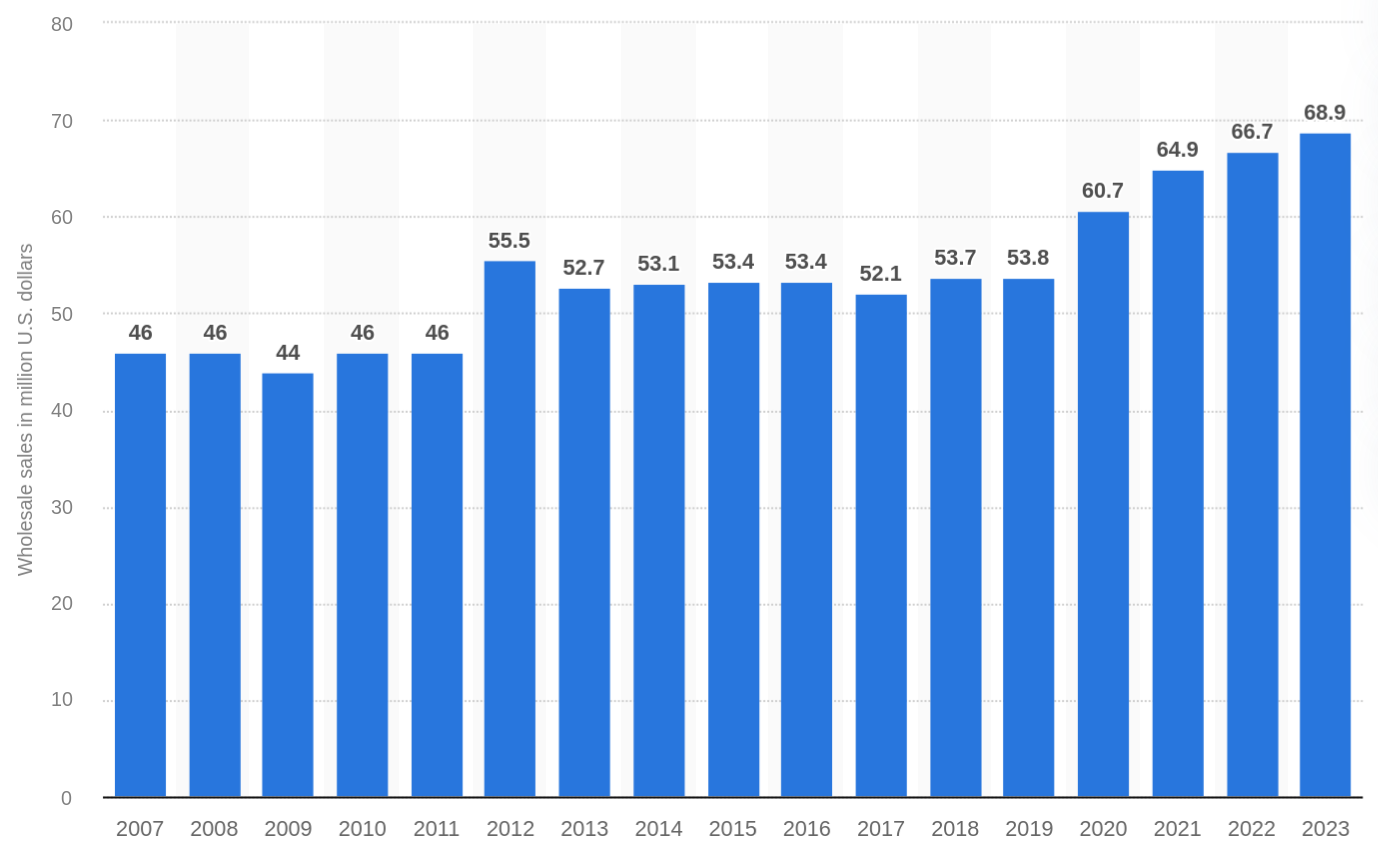
\includegraphics[width=0.7\linewidth]{figures/wholesales.png}
    \caption{Table tennis equipment wholesale sales in the U.S. from 2007 to 2023 \cite{statista2024}}
    \label{fig:intro}
\end{figure}

For such a popular sport that spans from a professional and competitive scene to a leisure time hobby for a large demographic, a prominent issue may be expressed as its requirement of two people to be played. A willing partner to practice with may not be readily available at all times, and this poses a problem for both professional players who need to practice and hone their skills for competition, and the general population who seek to play it for various reasons ranging from pastime hobby to a healthy lifestyle. For this reason, the need for a product that allows people to practice the sport on their own is apparent. However, the already existent products on the market are either too expensive to serve a broader customer population or lack some features that may result in a poorer experience. This project aims to fill the gap and create a table tennis ball pitching machine suitable for players of all skill levels, from amateur to professional.

To accomplish this goal and imitate a real play experience as closely as possible, certain requirements should be met. These requirements include but are not limited to, the machine being able to automatically adjust its yaw and pitch angles, perform simple and basic pitches while also being able to give various spin options, launch the ball at different speeds and frequencies, as well as switching between these variations automatically. The machine should also be able to store a minimum number of balls, and recycle successfully returned balls into the system via some mechanism. Considering these requirements, design specifications and criteria can be constructed as follows:

\begin{itemize}
    \item The ball must reach a maximum speed of 30 m/s during launch. It must be adjustable within this range.
    \item The ball’s launch frequency must provide 60 balls per minute. It must be adjustable within this range.
    \item The ball must be able to be given spin up to 500 RPM, including backspin, topspin, sidespin, and their derivatives. This spin value must be independent of speed.
    \item The launcher must provide launch with a yaw angle within a range of ±20 degrees horizontally.
    \item The launcher must provide launch with a pitch angle within a range of 0 to -20 degrees vertically.
    \item A storage area that can accommodate a minimum of 60 balls is required.
    \item The maximum weight of the entire system must not exceed 25 kilograms.
    \item The system is securely fastened to the table or floor in the middle of the opponent’s side of the ITTF standard table, at the center of the width of the table. The maximum displacement after 50 throws shall be 20 mm.
    \item The lifetime of a single ball in the cycle should be at least 1000 throws.
    \item The system must have a user interface allowing launch parameter configuration with a maximum 10\% deviation.
    \item The design can collect the properly returned balls from the player. Recyclable ball height needs to be at least 1 meter.
    \item The system is compliant with ITTF table and ball dimensions:
    \begin{itemize}
        \item Suitable for a 2.74 m long and 1.525 m wide table.
        \item Can serve over a 15.25 cm high net.
        \item Suitable for standard table tennis balls with a 2.7-gram weight and 40 mm diameter.
    \end{itemize}
    \item The machine should operate on standard mains electricity (220-240V, 50-60 Hz). Also, it should not consume more than 2000W.
    \item Total spending for the prototype of the design should be kept within 300 USD.
    \item The design, when unassembled, should fit inside a 1 m\textsuperscript{3} box.
    \item \textbf{(Bonus)} The ball must be able to be thrown without spin.
    \item \textbf{(Bonus)} The ball is first bounced by the shooter, giving the user the experience of serving.
\end{itemize}

\begin{table}[H]
\centering
\begin{tabular}{|c|p{7cm}|c|}
\hline
\textbf{\#} & \textbf{Design Criteria} & \textbf{Percentage} \\ \hline
1 & Serving Speed & 13\% \\ \hline
2 & Throwing Frequency & 13\% \\ \hline
3 & Spin Type and Amount & 10\% \\ \hline
4 & Yaw Angle Adjustment & 7\% \\ \hline
5 & Pitch Angle Adjustment & 7\% \\ \hline
6 & Storage Capacity & 6\% \\ \hline
7 & Weight & 4\% \\ \hline
8 & Stability of the System & 6\% \\ \hline
9 & Ball Durability & 4\% \\ \hline
10 & Control Accuracy and Output Consistency & 7\% \\ \hline
11 & Ball Recyclability & 5\% \\ \hline
12 & Compliancy with Standards & 3\% \\ \hline
13 & Power Consumption & 3\% \\ \hline
14 & Budget & 8\% \\ \hline
15 & Portability & 4\% \\ \hline
16 & No Spin Option (Bonus) & 5\% \\ \hline
17 & Special Serving (Bonus) & 5\% \\ \hline
\end{tabular}
\caption{Design Criteria and Their Percentages}
\label{tab:design_criteria}
\end{table}

The design for this project starts with a thorough literature survey conducted on products on the market, state-of-the-art technologies and patents related. Then, a detailed task distribution and management plan is done spanning the whole project process, which helps lay out a road map and makes it easier to organize and handle the work for further down the line. The conceptual design starts at this point, where ideas and concepts begin to appear, which are listed and evaluated using methods such as performing functional decomposition, creating a morphological chart and passing them through Analytical Hierarchy Process. After a best design is chosen through these processes, the detailed design part is initiated. In this part, necessary analyses and calculations are performed to justify the design, the test plans are made and test are carried out, and components and parts are manufactured accordingly. Optimization processes are done where necessary. At the end of this part, a fully assembled and working system is expected to be constructed. The whole design process is documented from start to finish, with important information such as technical drawings, cost analysis and sustainability report included, to create a clear and concise report so as the design process and the design itself could be understood. 

This final report is the combination of all the reports created up until this point for different parts of the design process. A discussion and conclusion is given at the end of the report, where the final product is discussed, and conclusions derived are mentioned. The references part, where the sources made use of and referred and the appendix part, where the necessary appendices are presented are also given at the end. The outline of the final report is given as,


\begin{enumerate}
    \item \textbf{Abstract}
    \item \textbf{Introduction}
    \item \textbf{Literature Survey}
    \begin{enumerate}
        \item[a.] Introduction
        \item[b.] Commercial Products
        \item[c.] State-of-the-art on Related Technologies
        \item[d.] Patents
        \item[e.] Summary and Conclusion
    \end{enumerate}
    \item \textbf{Project Planning and Management}
    \begin{enumerate}
        \item[a.] Introduction
        \item[b.] Organization of the Project
        \item[c.] Summary and Conclusion
    \end{enumerate}
    \item \textbf{Conceptual Design}
    \begin{enumerate}
        \item[a.] Introduction
        \item[b.] Concept Development and Presentation
        \item[c.] Evaluation of Concepts
        \item[d.] Best Concept
        \item[e.] Summary and Conclusion
    \end{enumerate}
    \item \textbf{Detailed Design}
    \begin{enumerate}
        \item[a.] Introduction
        \item[b.] Properties of the Designed System
        \item[c.] Engineering Calculations
        \item[d.] Analysis Results
        \item[e.] Discussion of Control Algorithms and Software
        \item[f.] Optimization
        \item[g.] System to be Manufactured
        \item[h.] Sustainability Analysis
        \item[i.] Test Plan
        \item[j.] Standards Used for Design Procedures and Performance Evaluation
        \item[k.] Discussion and Conclusion
    \end{enumerate}
    \item \textbf{Discussion}
    \item \textbf{Conclusion}
    \item \textbf{References}
    \item \textbf{Appendix}
\end{enumerate}

\chapter{Literature Survey}

% Main title and keyword section
\begin{center}
    \vspace{1em} % Add some space
    \vspace{1em} % Add some space
    \textbf{KEYWORDS: Table Tennis, Ball Thrower, Ball Collector, Trajectory Control, Ping Pong Spin}
\end{center}

% Start of sections
\section{Introduction}

For this project of a table tennis pitching machine, a detailed literature survey that includes the research of commercial products available in the market, state of the art technologies and the patents is conducted. As the market for table tennis is wide and open for profit, there are already numerous of products and technologies on how to approach different aspects of the project.\\

For commercial products, different table tennis ball pitching machines on the market are observed and analyzed to get an idea about their capabilities and shortcomings. It is necessary to choose which features to implement based on the demand of the market and the cost-effectiveness of the end product. \\

The state-of-the-art technologies are plenty for this project at hand, as there are multiple functions the machine must be able to perform. For aspects of launching, feeding itself from a reservoir, adjusting the speed and frequency etc., different kind of devices and mechanisms that can be used are investigated. \\

Lastly, patents are an important part of the research, as intellectual properties must be respected, and should be taken into consideration so as to ensure the proceeding of the project does not raise any issues with copyright infringement.

\section{Commercial Products}

\begin{minipage}{0.6\textwidth}
    The table tennis table market is a vibrant sector in the sports and recreation sector, appealing to a variety of consumers from amateur players to professional athletes. The statistics in Figure \ref{fig:commer1} below show the sales figures of table tennis equipment from manufacturers in the United States from 2007 to 2023. Last year, total sales of table tennis equipment in the United States reached approximately \$69 million in 2023. This was an increase of approximately 28\% compared to 2019. Therefore, it is naturally expected that the number of products and manufacturers in the market will increase. Also, according to research conducted by Business Research Insights, the global table tennis table market size was USD 485.3 million in 2022 and the market is expected to reach USD 598.11 million by 2032, growing at a CAGR of 2.1\% during the forecast period \cite{table_tennis_market_2032}.
\end{minipage}
\begin{minipage}{0.38\textwidth}
    \centering
    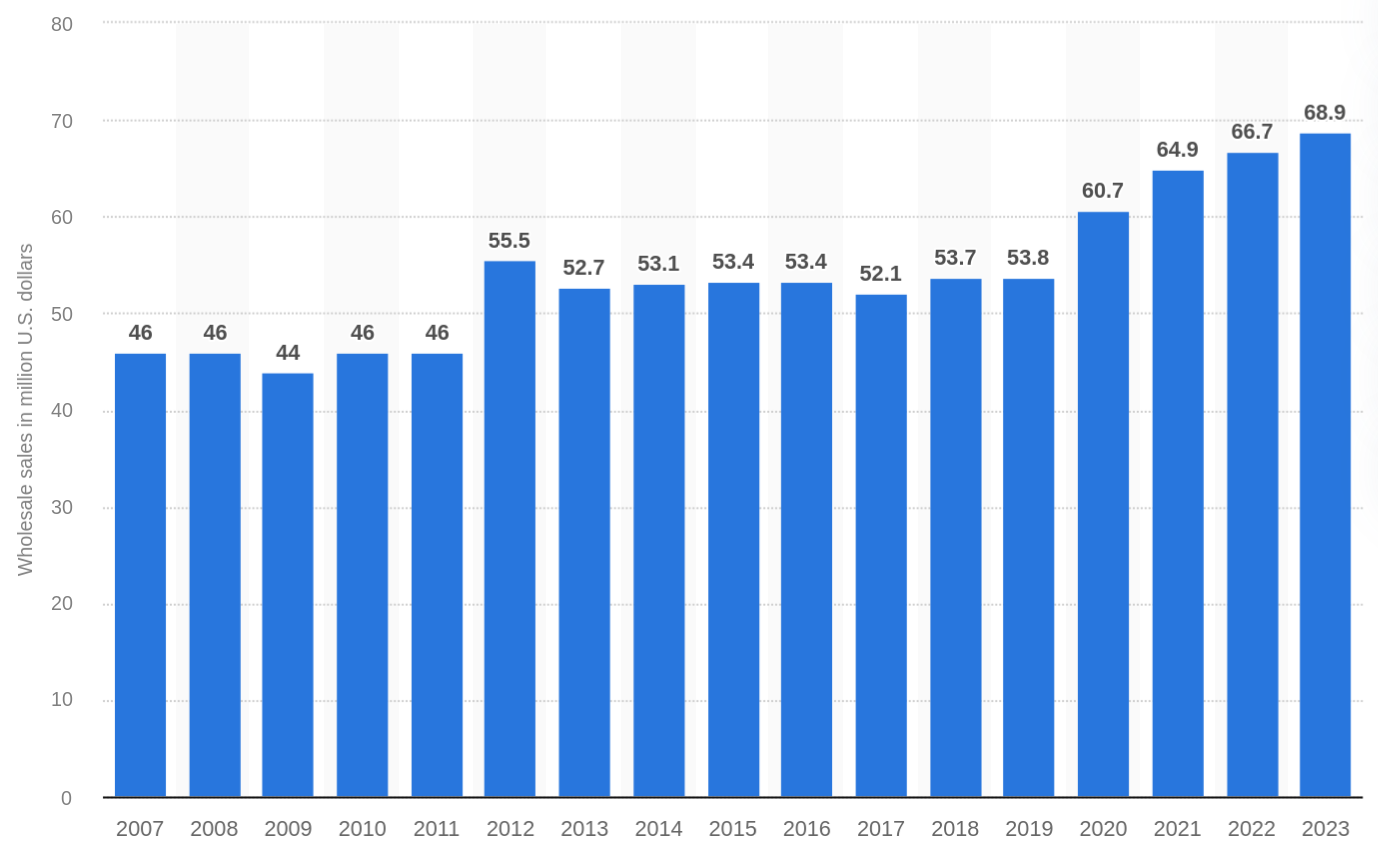
\includegraphics[width=\textwidth]{figures/wholesales.png}
    \captionof{figure}{Table tennis equipment wholesale sales in the U.S. from 2007 to 2023 \cite{statista2024}}
    \label{fig:commer1}
\end{minipage}



After careful research, various table tennis ball launcher models starting from \$100 and going up to \$2500 are found. One can see some common models, along with their comparisons in Table \ref{commercial} in Appendix. Of course, there are many differences in features among the devices in this wide price range. While affordable models can launch the ball without turning or by turning it only in one direction, advanced models can send the ball by turning it in 36 different ways. On the contrary, the dimensions of the ball chambers and the launch speeds are independent of the product prices. Almost all of the products, regardless of their prices, have launch speeds between 4 and 40 m/s. \\

In terms of usage, many products have wired or wireless control units. These units provide limited access with the buttons on them. It is seen that only in the highest segment products, the controller is in the form of a phone application. This feature should not be such a luxurious feature. This development may be a situation that is welcomed by many users. In addition, while doing this research it is seen that the ball turning mechanisms of various models are the same. Since the mechanism was the same, different rotations could not be obtained, but the number of rotations was increased by rotating the head section with smaller intervals. The research also shows that the products in this area could be further improved. \\

Several commercial products that serve the same purpose as the project requirements are reviewed. Most of the products are at an acceptable level at meeting the requirements but none of them fully meets the wanted requirements. The required max serving speed of 90 m/s couldn’t be achieved by any of the products. The max achieved speed is 40 m/s. One of the key requirements, the launch frequency, was almost achieved by most products, but fully achieved only by 4 products. These are the products of RoboPong and PowerPong. Considering the overall performance one can see that Robo Pong Super Pro and Robo Pong Pro Digital are the most suitable ones for the project requirements.

\section{State-of-the-Art on Related Technologies}

Recent developments in table tennis ball launchers, outlined in this section, focus on enhancing training efficiency and replicating real-game conditions. The literature survey identifies various studies exploring launch mechanisms and ball feeding systems that improve precision and control over key parameters. These advancements enable more precise training experiences, allowing players to better prepare for actual gameplay. This section states the findings from the literature on the latest innovations in table tennis ball launchers, highlighting their technical specifications and proposing directions for future research and development. 

\subsection{Launch Mechanisms}


Over the years, various pitching mechanisms have been developed, each with unique features designed to cater to different training needs. Among the most common are wheeled, pressurized, and hammered pitching machines  \cite{Lan2024}. Each mechanism offers different benefits, like precise control over ball speed, ability to give spin, adjust ball trajectory or realistic human-like trajectories. Understanding the differences in these machines’ mechanisms is crucial for selecting the right one to suit specific requirements of the project. 

\begin{indentedsection}

\subsubsection{Wheeled Pitching Machines}

Wheeled pitching machines utilize two or more spinning wheels to grip and propel the ball. The speed of the wheels can be adjusted independently, allowing for precise control over both speed and spin \cite{Dittrich2023}. By controlling the rotation speed of each wheel, users can simulate a variety of pitches making wheeled machines suitable for the project. Their ability to precisely control the trajectory, speed, and spin of the ball makes them a popular choice for both professional and amateur training environments (\cite{zxmoto2022}, \cite{amazon2024}, \cite{ipong2022} etc.). These mechanisms are also easier to manufacture compared to other pitching methods since the only moving parts are the wheels that accelerate the ball \cite{Zhang2021}.

\subsubsection{Pressurized Pitching Machines}

Pressurized pitching machines function by using a compressed air system to propel the ball \cite{Wiley1994}. These machines are known for their ability to achieve very high ball speeds, which makes them ideal for practicing fastballs. However, they are limited in their ability to generate spin and control trajectory as effectively as wheeled machines. The air pressure can be adjusted to control the velocity of the pitch, but this type of machine is less versatile for training different types of pitches. Additionally, the need for a reliable air compressor makes these machines bulkier and less portable. 

\subsubsection{Hammered Pitching Machines}

Hammered pitching machines use a mechanical arm or hammer to strike and propel the ball forward. While this method simulates overarm throws or cricket bowling actions, it lacks the fine control over spin and speed that wheeled machines provide. These machines are often used for training where high consistency in delivery is necessary, but their lack of spin manipulation and limited speed control make them less effective for comprehensive training purposes. However, they offer a realistic simulation of  human-like throw, which may be advantageous in certain training scenarios. \\

\end{indentedsection}

Since wheeled mechanisms are superior in speed and trajectory control, the primary focus of the research was on these mechanisms and robots. There are various studies on different wheeled launch mechanisms in the literature. In the study of AIMY \cite{Dittrich2023}, they employed a three-wheel configuration to generate precise ball speeds, up to $15.4 m/s$, and spins up to $192.0 s^{-1}$, similar to professional human players.  Also, the study on table tennis robotic launchers \cite{Jamaludin2022} provides valuable insights into the development of launch mechanisms. The launch unit of table tennis robotic launchers predominantly employs one or two rotating wheels to propel the balls with variable speeds and spins. This system allows for precise control over ball velocities mTTTbot project utilizes two brushless motors connected to silicone wheels in the launch mechanism \cite{Tasci2023}. As noted by Jamaludin et al. \cite{Jamaludin2022}, the robot uses DC motors to generate spin and adjust the launching speed of the balls. By modifying the Pulse Width Modulation (PWM) values, the launch speed and distance can be controlled, which directly impacts the ball’s travel distance and spin during play. Apart from these, there are further studies in the literature not only specific to table tennis but also include diverse launch mechanisms which can also help us in our project. Distinct features in tennis ball machines, as described by Gao, contribute to the launch mechanisms \cite{Gao2019}. In Gao’s study, tennis balls are launched using two friction wheels with a 90 mm diameter and a 3 mm concave depth. These features improve grip and spin control, providing better ball speed and direction. The wheels are powered by 12V motors, allowing adjustable launch speeds and angles for versatile training. The concave design of the friction wheels enhances ball spin and control, making this design competitive with more expensive tennis ball machines.

\subsection{Ball Feeder}

The ball feeding system plays a critical role in maintaining a consistent and uninterrupted supply of balls to the launch mechanism, as demonstrated in several studies. The ball feeder in AIMY’s design offers precise control and reliability with its crank mechanism that converts the rotary motion of a servomotor into linear motion as shown in Fig.2, ensuring continuous feeding without clogging, which is ideal for long-duration training. However, the mechanical complexity may increase manufacturing and maintenance costs \cite{Dittrich2023}. Also, the table tennis robotic launcher described by Jamaludin et al. employs a hopper system that has a high ball storage capacity, between 100 and 300 balls. The balls are delivered via a motorized conveyor belt or a rotating crank system, allowing for adjustable feed rates ranging from 25 to 80 balls per minute \cite{Jamaludin2022}. Apart from these, the mTTTbot project introduces a servo-driven feeding mechanism that continuously delivers balls through a helical channel, preventing interruptions in the training flow. As a drawback, its reliance on continuous servo control could limit durability during extended use \cite{Tasci2023}. According to another study by Jamaludin et al., the ball feeder is driven by a motorized mechanism that supplies balls at a rate of 8 to 15 balls per minute under stationary conditions, although this rate decreases when the robot rotates to aim at different angles \cite{Jamaludin2023}. Expanding on the design concepts, Gao’s research on tennis ball machines includes a turntable mechanism that feeds balls into a guide rail with improved timing and frequency control. This system also prevents blockage between layers, enhancing the reliability of the feeding process during extended practice sessions \cite{Gao2019}. 

\vspace{0.5cm}\begin{figure}[H]
\centering
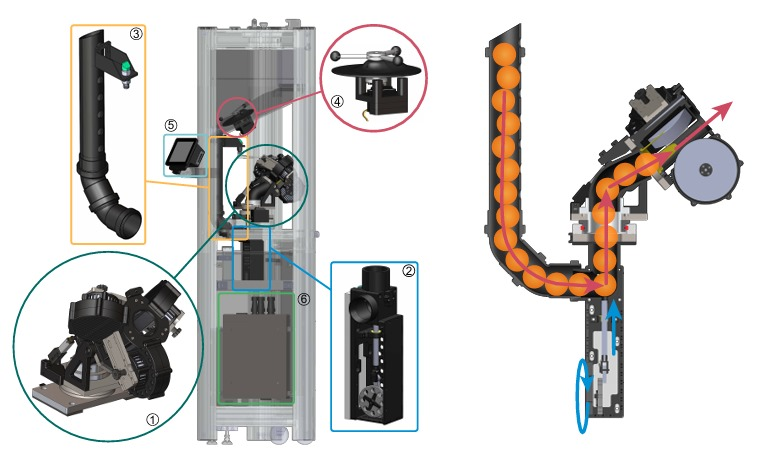
\includegraphics[width=0.45\textwidth,height=0.26\textwidth]{figures/fig2.jpg}
\caption{Sectional view of the ball feeding flow from the reservoir to launch unit in AIMY \cite{Dittrich2023}}
\end{figure}

\subsection{Reservoir}

The reservoir component plays an essential role in ensuring a continuous and uninterrupted supply of balls to the feeding system in robotic launchers. AIMY’s ball feeding system includes an optical sensor that monitors the ball supply and activates a stirrer to prevent clogging, ensuring a smooth flow of balls to the launch unit \cite{Dittrich2023}. In table tennis robotic launchers, as described by Jamaludin et al., the reservoir is designed to store a large number of balls (ranging from 100 to 300) and incorporates mechanisms to prevent clogging, ensuring consistent feeding to the launcher [2]. The mTTTbot system also features a ball reservoir that stores balls before feeding them into the launcher. A stirrer mechanism is integrated to prevent jams, further enhancing the operational reliability of the robot during training sessions [3]. In a study by Jamaludin et al., the ball reservoir is also equipped with a stirrer mechanism to prevent any clogging issues, like the AIMY robot [4]. In the case of tennis ball machines, Gao describes the use of a turntable reservoir with a two-layer design, which can hold up to 12 balls at once. While this design helps to avoid blockages between layers and ensures a smooth feeding process, its limited capacity may require more frequent reloading during prolonged practice sessions [5]. 

\subsection{Control Unit}

The control system is a pivotal component in the functionality of robotic ball launchers, allowing precise adjustments and remote management of the launch parameters. AIMY utilizes a Raspberry Pi as its control unit, enabling low-latency control (500 ms) through Ethernet or Wi-Fi, and providing an interface for integration with reinforcement learning (RL) environments via a Python API [1]. In a related study on table tennis robotic launchers, Jamaludin et al. describe the use of advanced user interfaces, which can be integrated with smartphone applications to control the system wirelessly via Bluetooth or Wi-Fi. These interfaces allow users to pre-program training routines and adjust variables such as spin, speed, and ball frequency for enhanced training realism [2]. The mTTTbot project also adopts an electronic control system that includes motor drivers, Bluetooth communication for remote control, and a microcontroller to manage all functions. The user-friendly mobile app interface facilitates easy adjustments of motor speeds, spin types, and shot angles, offering high flexibility for different training scenarios [3]. Jamaludin et al. further elaborate on an Arduino-based control system that manages the motors and movements, which is paired with a Bluetooth module for smartphone-based wireless control. This system leverages PWM control to fine-tune the speed and power supplied to the DC motors, enabling precise adjustments to the ball’s launch speed and travel distance [4]. Similarly, in the field of tennis ball machines, Gao’s research demonstrates the use of an STM32F407 microcontroller, which allows users to customize launch parameters such as speed, angle, and frequency, offering a highly responsive and versatile control experience [5].

\subsection{Actuators}

The selection and configuration of motors and actuators are crucial for controlling both the speed and spin of the balls in robotic launchers. AIMY utilizes high-performance brushless motors (T-MOTOR Antigravity MN5008 KV170) and servo motors to control the orientation and speed of the launch unit and ball feeding mechanism [1]. Similarly, in the table tennis robotic launcher described by Jamaludin et al., brushless motors are responsible for adjusting ball velocity and spin, while servo motors control the trajectory and launch angle to ensure precise delivery of balls during training sessions [2]. In the case of the mTTTbot, the launch unit operates with two brushless motors connected to silicone wheels, allowing for the generation of different types of spins, such as topspin, backspin, and sidespin, by adjusting the motor speeds [3]. Additionally, servo motors control the pitch, yaw, and roll axes of the launch head, providing precise adjustments for shot placement. According to Jamaludin et al., the robot uses DC motors to generate ball spin and adjust launch speed through Pulse Width Modulation (PWM) values, enabling fine-tuned control over ball travel distance [4]. Extending this approach to tennis ball machines, Gao’s research highlights the use of 12V DC motors that drive friction wheels with a concave design, enhancing ball grip and control over velocity and spin [5]. This combination of motors and actuators across different studies underlines their importance in achieving high precision and consistency in robotic launchers.



\vspace{1cm}In this state-of-the-art section, a comprehensive review of recent developments in table tennis ball launchers was conducted to inform the design of the project. In addition to that their advantages and disadvantages are discussed. Key mechanisms, including wheeled, pressurized, and hammered pitching systems, were analyzed to understand their respective strengths and limitations regarding speed, spin, and trajectory control. Ball feeding systems were explored to ensure continuous, jam-free ball supply for uninterrupted practice, while control units and actuator technologies were examined to enable precise adjustments and enhance the overall accuracy of ball delivery.  By studying these technologies, the most suitable components and designs for creating an efficient, adaptable, and realistic table tennis training system were identified. 

 
\section{Patents}
In this section, a review of existing patents related to table tennis ball launching machines is presented. This analysis aims to highlight innovative design approaches and technologies that were previously patented. By examining these patents, it is ensured that the design remains compliant with intellectual property laws while gaining insights into potential solutions that could inspire and guide the development of the project.
\subsection{Table Tennis Robot (US4765618A) \cite{Daley1988}}

\begin{minipage}{0.6\textwidth}  % Text takes 70% of the width
    This table tennis robot design aims to serve the ping-pong ball continuously at adjustable directions and methods, such as top-spin, back,and side-spins. This approach provides a more comfortable experience while practicing. The main idea here, which may be helpful, is that the balls are brought from bottom to top (from a lower level to a higher level), released to the serving mechanism and this procedure is continuously repeated. The serving mechanism consists of wheels to direct the balls. To accelerate the balls and satisfy the speed criteria, the design could be useful. However, on the other hand, depending on the elevation of the ball reservoir, the power consumption may be excessive and the design may be inconvenient. If the elevation is too high, the power needed to lift the balls could be quite high. To sum up, depending on the process and needs, this design could be beneficial and logical to implement.
\end{minipage}%
\hfill
\begin{minipage}{0.38\textwidth}  % Figure takes 28% of the width
    \centering
    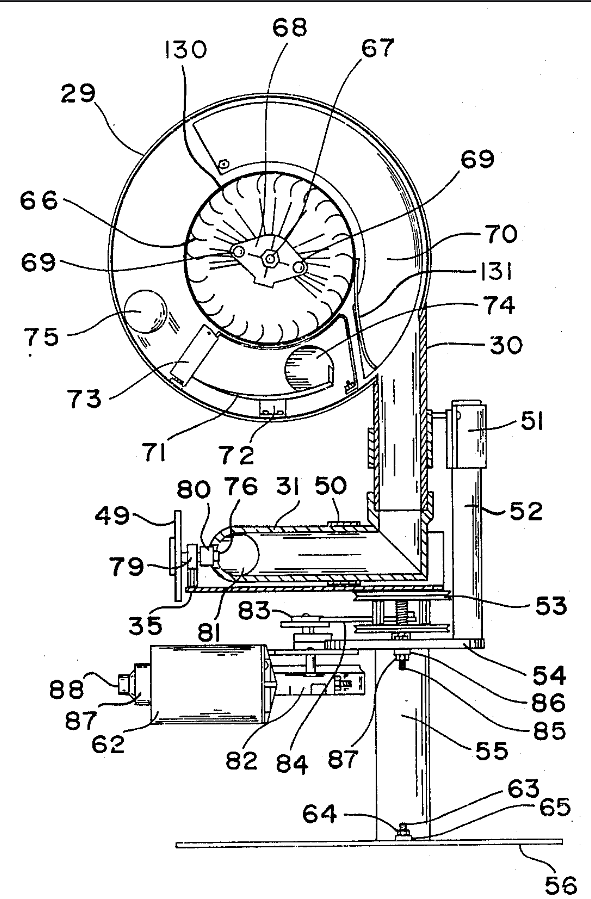
\includegraphics[width=0.47\textwidth]{figures/patent1-2.png}  % First image (48% width)
    \hfill
    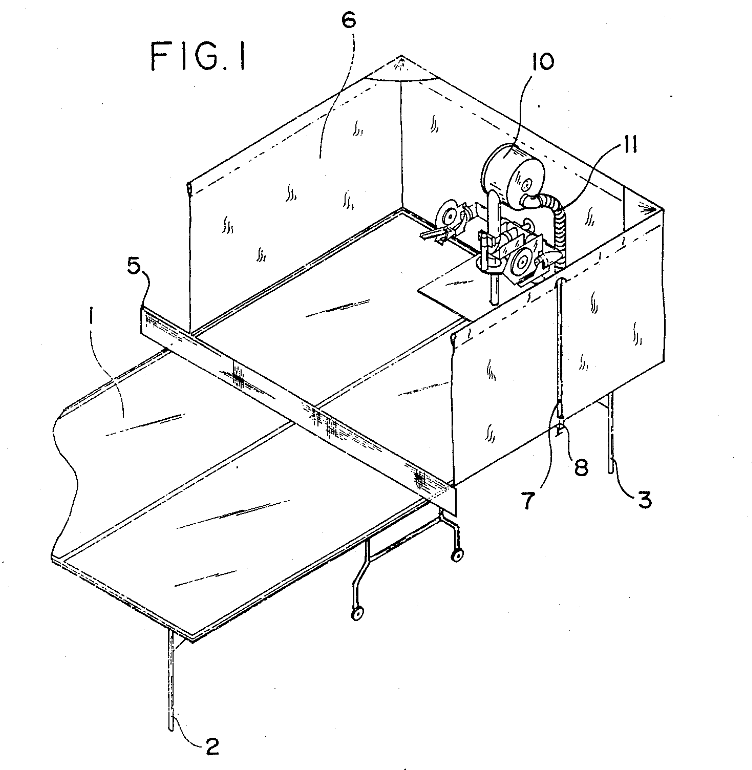
\includegraphics[width=0.48\textwidth,height=0.68\textwidth]{figures/patent1-1.png}  % Second image (48% width)
    \captionof{figure}{General System Description \cite{Daley1988}}  % Caption for both images
    \label{fig:pt1-2}
\end{minipage}


\subsection{Table Tennis Serving Machine (US6604517B1) \cite{Chao2003}}

\begin{minipage}{0.7\textwidth}  % Text takes 70% of the width
    This design is a much simpler and more non-complex example of an approach while constructing a table tennis robot for those who would like to exercise and train by themselves. It basically consists of a gear system, ball reservoir segments capable of carrying 2 balls simultaneously, and a spring system to throw the ball. If the priority is simplicity, this design could be useful. Also, to achieve the desired speed, a stiff spring system could be useful. The main underlying reason that this design is patentable is that it replaces electronic components with mechanical components. Therefore, this design provides more simplicity. However, in terms of longevity, practicality, and ergonomics, this design is probably not the most usable one. The possible wear of the gear system may make the design unusable in a couple of years. In addition, the gear system could make the design heavy and difficult to carry.
\end{minipage}%
\hfill
\begin{minipage}{0.28\textwidth}  % Figure takes 28% of the width
    \centering
    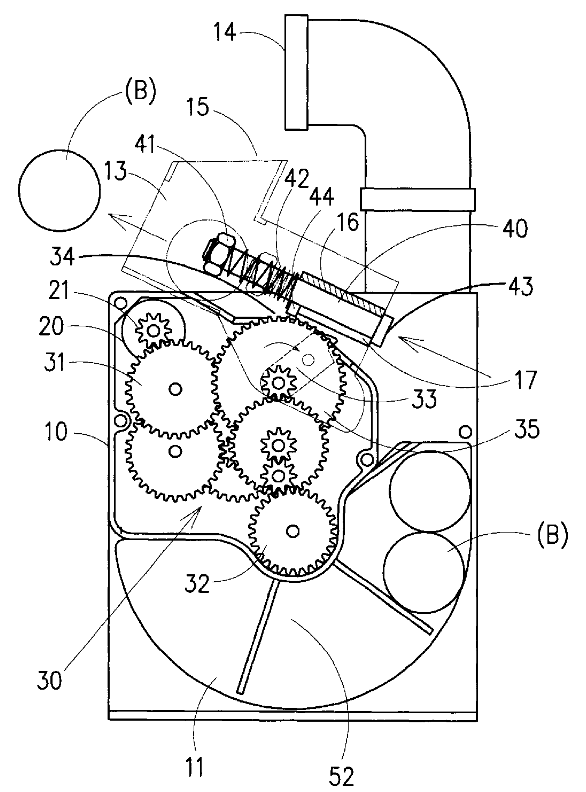
\includegraphics[width=\textwidth]{figures/patent2-1.png}
    \captionof{figure}{General schematic of serving machine \cite{Chao2003}}
    \label{fig:pt2-1}
\end{minipage}


\subsection{ Table Tennis Robot with Improved Serving Head Movement
 (EP3967376A1) \cite{Thoman2022}}

\begin{minipage}{0.7\textwidth}  % Text takes 70% of the width
     At that design, a ball feed collector can be seen. The main difference from the first design is that the internal pipe raises the balls to be able to throw them and this design raises the balls in a more effective way since the ball collector reservoir is lower, which could be a key point for a good design. There are several servo motors and gears to adjust the thrower part. To exemplify, the thrower is able to move upwards and downwards, depending on the process desired, which enables the practice to have a more realistic experience. Also, the thrower part is adjustable so that the ball can be manipulated to make a top-spin, back-spin, and side-spin type of throws. By the gear system, the angle of the thrower becomes adjustable. 
\end{minipage}%
\hfill
\begin{minipage}{0.28\textwidth}  % Figure takes 28% of the width
    \centering
    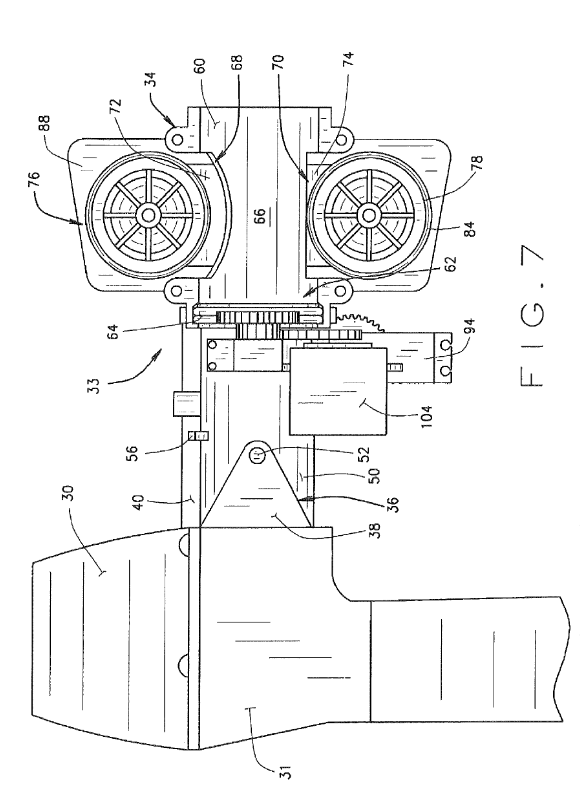
\includegraphics[width=0.9\textwidth]{figures/patent3-3.png}
    \captionof{figure}{Side view and detailed mechanism of table tennis robot \cite{Thoman2022}}
    \label{fig:pt3-1}
\end{minipage}

\begin{figure}[H]
    \centering
    \begin{subfigure}{0.4\textwidth}
        \centering
        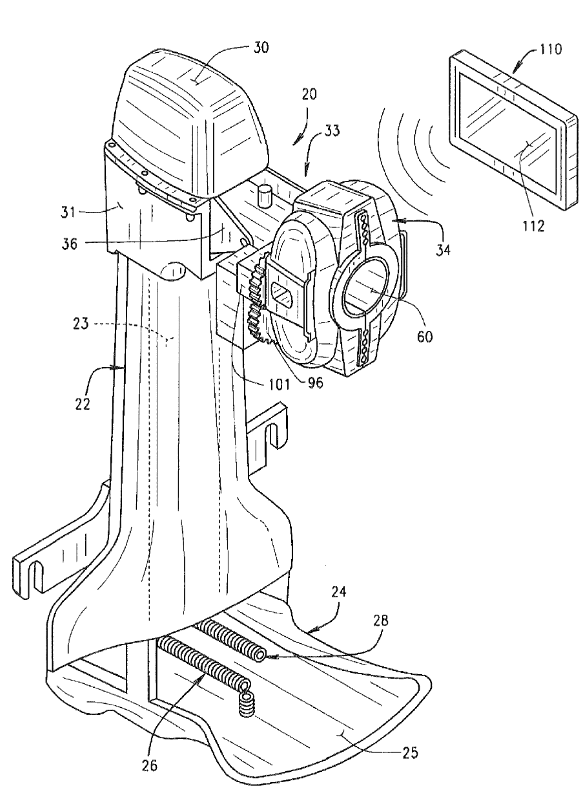
\includegraphics[width=0.45\textwidth]{figures/patent3-1.png}
        \caption{Orthogonal view}
    \end{subfigure}
    \hfill
    \begin{subfigure}{0.4\textwidth}
        \centering
        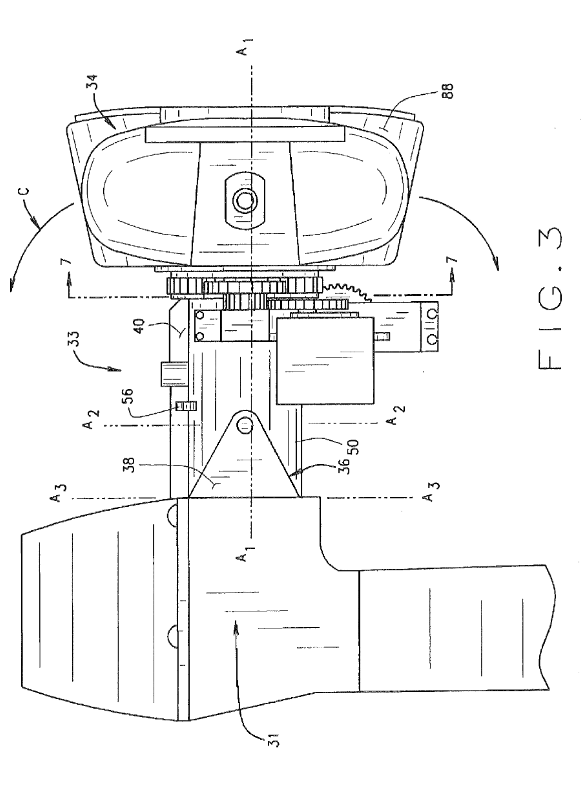
\includegraphics[width=.45\textwidth]{figures/patent3-2.png}
        \caption{General view}
    \end{subfigure}
    \caption{Orthogonal and general views of the table tennis robot \cite{Thoman2022}}
\label{fig:patetn3-2}
\end{figure}

\subsection{Programmable Ball Throwing Aparatus (US008287.4042B2) \cite{Romulo2012}}

\begin{minipage}{0.6\textwidth}  % Text takes 70% of the width
    In this device flight characteristics and field position parameters: spin, speed, ball trajectory are either programmed or manually selected by the user. The design is computer implemented and has built-in programs for different levels from beginner to expert. Also, it has specific modes for specific skill training like extreme backspin case. In addition, it allows users to program custom routines. The importance of this device for the project is that the planned product will also be adjustable for different flight parameters and trajectories. The underlying reason that this design is patentable comes from its programmability and freedom provided to the user.
\end{minipage}%
\hfill
\begin{minipage}{0.38\textwidth}  % Figure takes 28% of the width
    \centering
    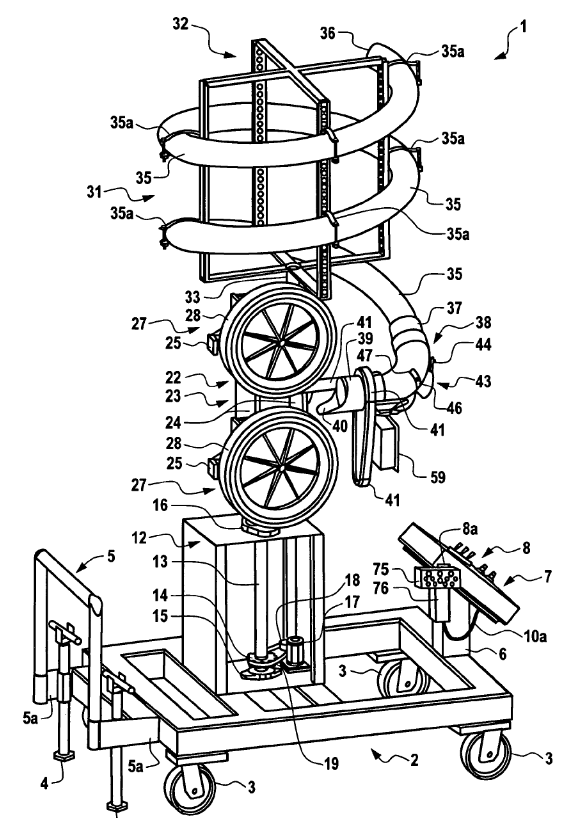
\includegraphics[width=0.48\textwidth]{figures/patent4-1.png}  % First image (48% width)
    \hfill
    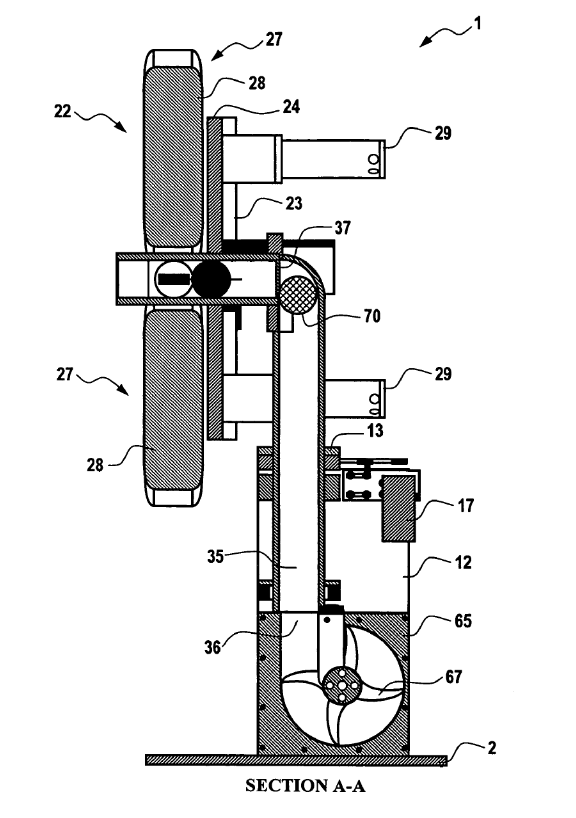
\includegraphics[width=0.48\textwidth]{figures/patent4-2.png}  % Second image (48% width)
    \captionof{figure}{General System Description \cite{Romulo2012}}  % Caption for both images
    \label{fig:patent4-1}
\end{minipage}

\subsection{Ball Throwing Device for Table Tennis (KR101992961B1) \cite{Kang2019}}

\begin{minipage}{0.6\textwidth}  % Text takes 70% of the width
    This patent describes a ball-throwing machine specifically designed for table tennis. The machine incorporates servomotors and various gears to control the ball's speed, spin, and direction. One key feature is its ability to continuously feed balls from a lower-level reservoir, reducing the machine's power consumption compared to designs with higher reservoirs. The ball thrower is adjustable for multiple spins (e.g., top-spin, back-spin), and the throwing mechanism is capable of providing angular adjustments for different ball trajectories. On the other hand, since the system can be constructed only once and it is not dispensable, this design may not meet the ergonomy criterion. 
\end{minipage}%
\hfill
\begin{minipage}{0.38\textwidth}  % Figure takes 28% of the width
    \centering
    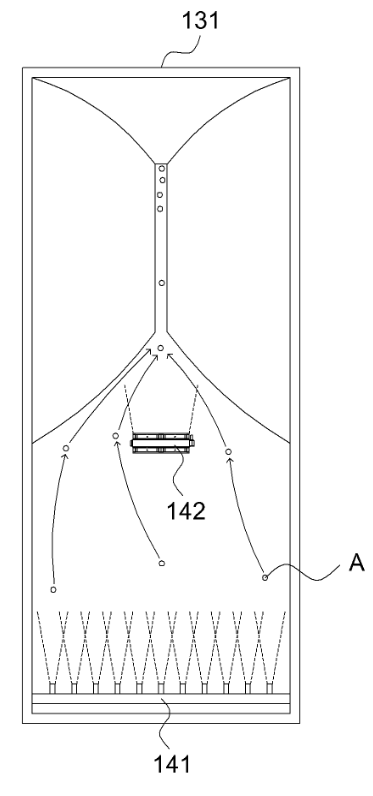
\includegraphics[width=0.48\textwidth,height=0.68\textwidth]{figures/patent5-1.png}  % First image (48% width)
    \hfill
    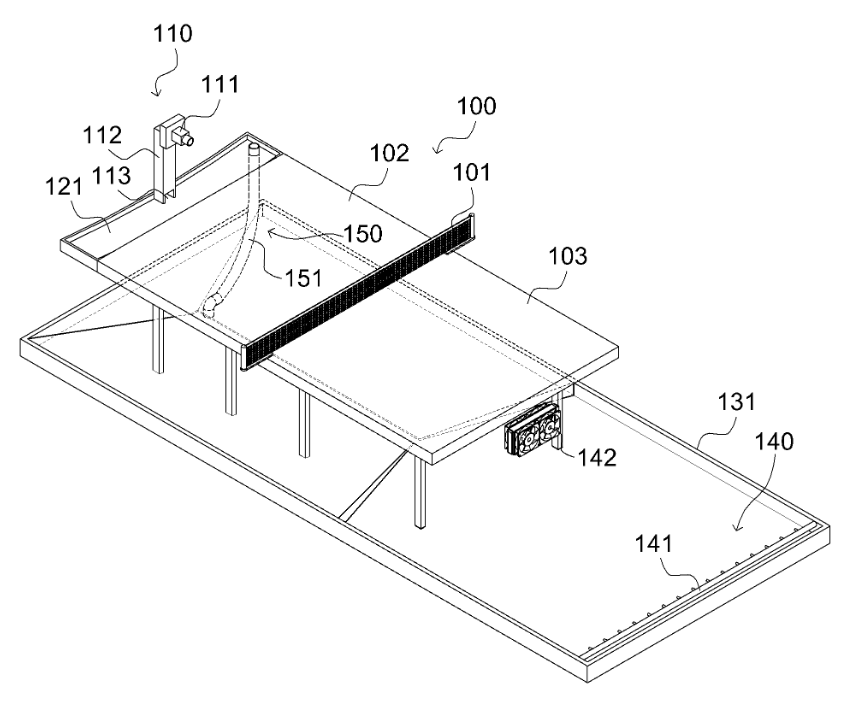
\includegraphics[width=0.48\textwidth,,height=0.78\textwidth]{figures/patent5-2.png}  % Second image (48% width)
    \captionof{figure}{Lower to Upper-Level Reservoir Feeding System \cite{Kang2019}}  % Caption for both images
    \label{fig:patent5-1}
\end{minipage}
\vspace{10pt}\\

The possible outcome of the research is, each of the designs has its advantages and disadvantages. The main idea is to be able to assess these designs wisely, get the ideas and inspiring points.


\section{Summary and Conclusion}
In this report, the results of a literature survey conducted spanning the commercial products in the market, state-of-the-art technologies and patents regarding the project at hand are presented. \\

A total of 10 commercial products are mentioned ranging from simple mechanical designs to highly advanced systems incorporating smart controls, whose different capabilities and aspects are studied to analyze their functions most useful to the project, and their shortcomings are discussed so as to how they could be improved upon, or be replaced with alternative solutions altogether. \\

State-of-the-art research made available many technologies and ideas that approach the technical problems encountered from different angles, and offer varying solutions to how the mechanisms operate. These different mechanisms are presented in detail to better understand their respective strengths and limitations regarding many technical aspects such as spin options, trajectory control, jam-free ball supply, enabling precise adjustments and accuracy. \\

A number of 5 patents are listed in this report, whose similarities and differences are discussed. Patents’ innovative approaches and methodologies to technical requirements including but not limited to power consumption, reserving and collecting the balls are mentioned to draw inspiration and compare the advantages and disadvantages of these designs. \\

In general, the information and ideas obtained from these research areas both gave rise to new inspiration and resulted in familiarizing with the many alternative solutions, while at the same time making apparent the need for a product to work upon the shortcomings and improve upon the strengths of the available designs to better simulate a real-life table tennis experience, thus enhancing the belief that this project will have a meaningful contribution to its field, and reinforcing the motivation to further work on it.

\newpage

\begin{sidewaystable}[h]
\centering
\scriptsize % Reduce font size
\begin{adjustbox}{width=\textwidth} % Scale the table to the text width
\begin{tabularx}{\textwidth}{|>{\centering\arraybackslash}X|>{\centering\arraybackslash}X|>{\centering\arraybackslash}X|>{\centering\arraybackslash}X|>{\centering\arraybackslash}X|>{\centering\arraybackslash}X|>{\centering\arraybackslash}X|>{\centering\arraybackslash}X|>{\centering\arraybackslash}X|>{\centering\arraybackslash}X|>{\centering\arraybackslash}X|}
\hline
\textbf{} & \textbf{PongBot Nova S Pro \cite{pongbotnova2024}} & \textbf{PowerPong Alpha \cite{powerpongalpha}} & \textbf{PowerPong Omega \cite{powerpongomega}} & \textbf{Huipang HP-07 \cite{huipanghp07}} & \textbf{Huipang S8-PRO \cite{huipangs8pro}} & \textbf{Huipang S1001 \cite{huipangs1001}} & \textbf{iPong V300 \cite{ipongv300}} & \textbf{Robo Pong Super Pro (3050) \cite{ipong2022}} & \textbf{Robo Pong Pro Digital (2055) \cite{robopong2055}} & \textbf{SIBOASI T899 \cite{siboasit899}} \\ \hline
\textbf{Price (USD)} & 350 & 1450 & 2195 & 256 & 763 & 172 & 140 & 2200 & 700 & 408 \\ \hline
\textbf{Length (cm)} & 46.5 & 24.1 & 24.1 & 39.4 & 88 & 41 & 28 & 28 & 28 & 165 \\ \hline
\textbf{Width (cm)} & 17.6 & 32.4 & 32.4 & 37.6 & 40 & 36 & 28 & 35.6 & 35.6 & 150 \\ \hline
\textbf{Height (cm)} & 34 & 78.7 & 78.7 & 35.8 & 41 & 32 & 48 & 83.8 & 83.8 & 78 \\ \hline
\textbf{Mass (kg)} & 4 & 10.89 & 10.89 & 4.42 & 7.5 & 4 & 1.25 & 8.15 & 10.9 & 5.4 \\ \hline
\textbf{Power (W)} & 24 & 24 & 24 & 36 & 50 & 36 & 50 & 50 & 50 & 60 \\ \hline
\textbf{Ball Frequency (balls per minute)} & 30-90 & 5-100 & 5-120 & 40-70 & 35-80 & 32-80 & up to 90 & 1-120 & 1-170 & 30-90 \\ \hline
\textbf{Ball Speed (m/s)} & 2-15 & 1-19 & 1-25 & 4-40 & 4-40 & 4-40 & 4-40 & 4-40 & 4-40 & 4-40 \\ \hline
\textbf{Capacity (balls)} & 200 & 100 & 100 & 120 & 200 & 120 & 100 & 120 & 120 & 80 \\ \hline
\textbf{No of spins} & 8 & 5 for topspin, 4 for backspin, 4 for right sidespin, 4 for left sidespin. & 7 for topspin, 5 for backspin, 6 for right sidespin, 6 for left sidespin. & 9 different spin options & 9 different spin options and no spin & 9 different spin options and no spin & 2 (Only Topspin and Backspin) & Topspin, Backspin, variety of side spins and no spin option & Topspin, Backspin, variety of side spins and no spin option & 4 \\ \hline
\textbf{Type of controller} & Mobile app + wireless remote controller & Control box and connects with a thin, light cable & No control box / Tablet or phone app can be used & Wired control box & Wireless remote & Wired control box & Wireless remote + digital panel & Mobile Application/Bluetooth & Digital Control box & Remote control \\ \hline
\textbf{Catch net to recycle balls} & - & + & + & - & + & - & - & + & + & + \\ \hline
\textbf{Material} & German BASF materials & Rubber + Metal & Rubber + Metal & Acrylonitrite butadiene styrene & Plastic + Metal & Plastic + Metal & Metal & Plastic + Metal & Plastic + Metal & Plastic + Metal \\ \hline
\textbf{Features} & \begin{itemize}[noitemsep, left=0pt, align=left]
    \tiny
    \item 20 to 30 up and down trajectory control
    \item Can be placed at 9 different positions on table
    \item Customizable spin, frequency, speed, oscillation, and trajectory settings
    \item Trajectory visualization on app
\end{itemize} & \begin{itemize}[noitemsep, left=0pt, align=left]
    \tiny
    \item 3 motors 120° degrees separated
    \item Allows many different shot types
    \item Has memory slots for shots
    \item Automatic Frequency Control
\end{itemize} & \begin{itemize}[noitemsep, left=0pt, align=left]
    \tiny
    \item 3 motors 120° degrees separated
    \item Allows many different shot types
    \item Unlimited memory for shots
    \item Individual Frequency Control
    \item Delay/Break time
\end{itemize} & \begin{itemize}[noitemsep, left=0pt, align=left]
    \tiny
    \item Rotating head for different spin directions
    \item 3 modes for trajectory angle
    \item Includes special Huipang balls reduce friction 
\end{itemize} & \begin{itemize}[noitemsep, left=0pt, align=left]
    \tiny
    \item Rotating head for different spin directions
    \item Adjustable head for trajectory angle
    \item Includes special Huipang balls reduce friction 
    \item Preset long/short ball, serve style practice
\end{itemize} & \begin{itemize}[noitemsep, left=0pt, align=left]
    \tiny
    \item Double heads for different types of serves
    \item Includes special Huipang balls reduce friction 
    \item Can serve two balls simultaneously
    \item 3 head modes for trajectory angle
\end{itemize} & \begin{itemize}[noitemsep, left=0pt, align=left]
    \tiny
    \item Includes tilt stand to change ball trajectory
    \item Can stand on its own
    \item Easily transportable
\end{itemize} & \begin{itemize}[noitemsep, left=0pt, align=left]
    \tiny
    \item Rotating head for different spin directions
    \item Different difficulty levels (Beginner to advanced)
    \item Advanced launching options
    \item Indicator lights that’s shows spin force and direction
\end{itemize} & \begin{itemize}[noitemsep, left=0pt, align=left]
    \tiny
    \item Rotating head for different spin directions
    \item Manually adjustable vertical tilt angle
    \item Different difficulty levels (Beginner to advanced)
\end{itemize} & \begin{itemize}[noitemsep, left=0pt, align=left]
    \tiny
    \item Rotating head for different spin directions
    \item Suitable for middle line ball, forehand ball, backhand ball trainings
\end{itemize}\\ \hline
\end{tabularx}
\end{adjustbox}
\caption{Comparison of Table Tennis Robots}
\label{commercial}
\end{sidewaystable}

% Prevent floats from passing this point
\FloatBarrier


\chapter{Project Planning and Management}
\addcontentsline{toc}{chapter}{Project Planning and Management}
\setcounter{section}{0}
\renewcommand*{\theHsection}{chX.\the\value{section}}

% Start of sections

\section{Introduction}
This report presents the planning and organization for the management of the Table Tennis Ball Pitcher Machine project. A structured timetable is established to guide each project phase, from problem definition to testing, ensuring efficient workflow. This document details the planning approach, task distribution and timeline established to ensure systematic project execution. The project members responsible for the tasks are abbreviated as in Table \ref{tab:teammembere}.

\begin{table}[h!]
\centering
\begin{minipage}{0.45\textwidth}
    \centering
    \begin{tabular}{|c|c|}
    \hline
    \textbf{Name} & \textbf{Abbreviation}\\
    \hline
    Abdullah Can Seyhanlı &  ACS\\
    Altay Ata Ateş & AAA\\
    Arman Utku Aydın & AUA\\
    Abdullah Salih Taşdelen &  AST\\
    \hline
    \end{tabular}

\end{minipage}%
\hfill
\begin{minipage}{0.45\textwidth}
    \centering
    \begin{tabular}{|c|c|}
    \hline
    \textbf{Name} & \textbf{Abbreviation} \\
    \hline
    Bilal Açıksöz & BA\\
    Kutay Can Yapıcı & KCY\\
    Ömer Aslan & ÖA\\
    Özge Dilan Tuna & ÖDT\\
    Yunus Emre Özçelik & YEÖ\\
    \hline
    \end{tabular}    
\end{minipage}
    \caption{The Members of the Project}
    \label{tab:teammembere}
\end{table}

    
\section{Organization of the Project}

In this section of the report, the definition of tasks and the workload distribution among the team members are presented. As a first step, a literature survey is conducted to define the problem. After defining the problem project requirements and specifications are determined. In consideration of these steps, the functions of the project are decomposed. 

\subsection{Explanation of the Tasks and Their Definitions}

\subsubsection{Literature Survey}
At the start of a project, literature survey carries great importance so as to gather information about the related products and technologies available on the market. Also, research regarding the patents related to the project is conducted. Ultimately, the literature survey gives insight about the direction the project will take. \\

\paragraphs{\textbf{a. Commercial Product Research (AAA, AUA, BA})}
This section involves the research of the products on the market. Prices of these products, their design criteria and to what extent they satisfy the said criteria are evaluated. Studying the interest on the market regarding the field and products also contributes to the project. \\

\paragraphs{\textbf{b. State of the Art Research on Related Projects (ÖDT, AST, KCY)}}
In this part, scientific papers and technological advancements that are related to the project are researched. State of the art research, unlike the commercial product part, takes into consideration the technologies that are new and some cutting-edge, thereby allowing for more creative ideas and open-minded thinking. \\

\paragraphs{\textbf{c. Patent Research (ACS, YEÖ, ÖA)}}
Patent research is a very crucial step in a design process. A product created without researching and knowing the patented products related to the project beforehand is not viable. The components and the products similar to the design in mind must be determined.  

\subsubsection{Project Initiation}
The project needs to be initialized and worked over after the literature survey is completed. An investigation process should be completed by using a step-by-step approach. After all the steps are completed, the project is to be completely initiated. \\

\paragraphs{\textbf{a. Problem Definition (AAA, YEÖ)}}
A problem needs to be defined properly if a design is to be made as a solution. Determining the problem correctly and thoroughly is important and makes it easier to create a good design in the later stages of the process. \\

\paragraphs{\textbf{b. Project Requirements (ÖDT, KCY, ÖA)}}
 In this step the requirements that should be met and the functions the product must be able to perform are defined without giving the numerical constraints or any measurable limitations. \\
 
\paragraphs{\textbf{c. Design Specifications (BA, AUA)}}
The requirements specified on the previous step are defined numerically in this step. Functions the product must be able to perform and the restrictions it is subjected to are indicated in a quantitative way. \\

\paragraphs{\textbf{d. Design Criteria (ACS, AST)}}
In this step, the design criteria for the product should be stated, and the percent weight of importance for each of the criteria are assigned. 

\subsubsection{Functional Decomposition}
Functional decomposition is a process to separate an engineering solution/device into its subfunctions. It is created based on need statements which is the process of converting customer needs into solution neutral engineering actions. Each subfunction should be suitable for individual examination. After the functional decomposition is performed, each function is investigated to find suitable solutions. \\

\paragraphs{\textbf{a. Flow Chart (YEÖ, BA)}}
Flow chart is a type of functional chart which includes all the subfunctions from the main function to the subfunction in a logical or temporal order with material, information, and energy inputs. These subfunctions are grouped by considering a common function to be performed. For the given inputs the outputs are also determined, considering the conservation. \\

\paragraphs{\textbf{b. Function Tree Chart (YEÖ, AST, AAA)}}
Functional tree chat is another type of functional decomposition. Main difference from the flow chart is that function tree is designed with levels starting from the main function extending with relevant subfunctions till the solution of each subfunction. \\

\subsubsection{Project Planning}
It is crucial to plan the schedule the project properly. Insufficient planning may lead to many problems, such as production errors and delays of the reports. To be able to plan properly, it is important to know the members of the group well and assign them tasks according to their interests and knowledge areas. \\

\paragraphs{\textbf{a. Project Organization (ALL TEAM)}}
Project Organization as a task involves setting up the structure, roles, and processes necessary for a project to run efficiently and achieve its objectives. Project Organization is foundational to project success, as it sets up the necessary framework, team alignment, and resources to achieve project goals. \\

\paragraphs{\textbf{b. Task Explanation and Assignment (AUA)}}
At the start of a project, first step is to determine the tasks. The task definitions must be done clearly and in a way that fully encompasses what the task should achieve. So, it is easier to determine how to approach each task, and it is possible to assign them to the member that is most capable of undertaking it. \\

\paragraphs{\textbf{c. Timetable and Timeline Creation (AUA, AST)}}
Aside from assigning the tasks and setting their definitions, it is important to allocate the time to complete these tasks. To achieve it, a timetable should be constructed and it has to be ensured that it is followed properly. For the timeline, it is necessary to fill a Gantt chart with the durations decided at the timetable, including the specific dates. 

\subsubsection{Conceptual Design}
Conceptual design is mainly composed of two steps: concept generation and concept evaluation. \\

\paragraphs{\textbf{a. Morphological Chart (ALL TEAM)}}
Morphological chart is a chart where generated concepts that are considered to be logical solutions at first look are listed. It is a method for concept generation. This process is done for each sub-function obtained during the functional decomposition and listed in the morphological chart. Generated concepts are illustrated with sketches which are in conceptual level, not necessarily in the engineering level. All the concepts must be in the same level and should perform the function for sure. \\

\paragraphs{\textbf{b. Concept Evaluation (ALL TEAM)}}
At this step, the generated concepts which are listed in morphological chart are evaluated considering each engineering criteria, choosing from several types of evaluation methods. The concepts are then graded. The results obtained from this step determines the optimal solution/s for each sub-function.

\subsubsection{Detailed Design}
At this step, the process which have been theoretical up to this point and the generated concepts take its final shape and the product architecture is determined. All the design parameters are quantified and parts that will perform the functions take form. This step is highly iterative and requires good communication among the team. \\

\paragraphs{\textbf{a. Kinematic Design (YEÖ, ACS)}}
This process includes kinematic analysis, synthesis, and optimization for all parts and parameters of the system. It requires hand calculations and geometry-based software. \\

\paragraphs{\textbf{b. Static Analysis (YEÖ, AAA)}}
 This process includes structural analysis which includes material selection and stress analysis of the parts. It requires hand calculations and engineering software. \\
 
\paragraphs{\textbf{c. Geometric Analysis (AUA, BA)}} 
This process includes CAD modeling, and geometrical parameter determination. \\

\paragraphs{\textbf{d. Circuit Design (AST)}}
In this process the circuitry needed for the motor control, buttons, encoders etc. and also the voltage regulators will be designed. It is crucial for not harming any electrical/mechanical components.


\subsubsection{Manufacturing}
\paragraphs{\textbf{a. Procurement (AUA, AST)}}
After the analyses are complete, the materials chosen according to the market research conducted previously are to be supplied. Procuring the materials is a crucial part since manufacturing process cannot start without deciding on and obtaining the materials needed. \\

\paragraphs{\textbf{b. Determination of Manufacturing Methods (YEÖ, KCY)}}
Regarding the project requirements, design specifications and the materials, the suitable methods to manufacture the system are to be decided on. In this part, the priority is to provide the sustainability of the material life and to avoid possible excessive expenses.  \\

\paragraphs{\textbf{c. Producing the Parts (AAA, ÖA, BA)}}
The necessary parts are to be produced by applying the manufacturing methods determined at the previous part.  \\
 
\paragraphs{\textbf{d. Assembly (ACS, ÖDT)}}
In the assembly section, the produced parts are to be joined together to create the final product. \\

\paragraphs{\textbf{e. Quality Control (AST, AUA)}}

Quality control should be performed for each part produced to ensure the quality of the materials, make sure the standards are met, foresee the potential unexpected changes and deviations to avoid them as much as possible, and to increase the efficiency of the process. After the assembly is done, it is important to do a final quality control to obtain an overall result. 

\subsubsection{Documentation}

\paragraphs{\textbf{a. Reports (ALL TEAM)}}
From the beginning of the project, reports are to be written to record the project design procedure and explain the steps better. This part also makes it easier to plan the timeline and organize the time until the deadline. \\

\paragraphs{\textbf{b. Drawings (KCY, YEÖ, AUA)}}
It is important to have the drawings of each part of the system, which includes the tolerances, dimensions and constraints, in order to manufacture the parts designed. \\

\paragraphs{\textbf{c. Calculations (AST, ACS, ÖA)}}
The pre-design calculations should be included for speed, motion, power, space required and trajectory motion etc. to demonstrate that the solutions are viable for the project requirements. 
\newpage

% Repeat for each task (e.g., Detailed Design, Manufacturing, Documentation)

\subsection{Time Table}

\begin{table}[h!]
\centering
\begin{minipage}{0.45\textwidth}
    \centering
    \scriptsize
    \begin{tabular}{|c|c|c|}
    \hline
    \textbf{Task ID} & \textbf{Duration} & \textbf{Team Members} \\
    \hline
    1.a & 2 weeks & AAA, AUA, BA \\
    1.b & 2 weeks & ÖDT, AST, KCY \\
    1.c & 2 weeks & ACS, ÖA, YEÖ \\
    2.a & 1 week & AAA, YEÖ \\
    2.b & 1 week & ÖDT, KCY, ÖA \\
    2.c & 1 week & BA, AUA \\
    2.d & 1 week & ACS, AST \\
    3.a & 1 week & YEÖ, BA \\
    3.b & 2 weeks & YEÖ, AST, AAA \\
    4.a & 1 week & ALL TEAM \\
    4.b & 1 week & AUA \\
    4.c & 1 week & AUA, AST \\
    5.a & 2 weeks & ALL TEAM \\
    \hline
    \end{tabular}
\end{minipage}%
\hfill
\begin{minipage}{0.45\textwidth}
    \centering
    \scriptsize
    \begin{tabular}{|c|c|c|}
    \hline
    \textbf{Task ID} & \textbf{Duration} & \textbf{Team Members} \\
    \hline
    5.b & 1 week & ALL TEAM \\
    6.a & 2 weeks & YEÖ, ACS \\
    6.b & 2 weeks & YEÖ, AAA \\
    6.c & 2 weeks & AUA, BA \\
    6.d & 1 week & AST \\
    7.a & 2 weeks & AUA, AST \\
    7.b & 1 week & YEÖ, KCY \\
    7.c & 3 weeks & AAA, ÖA, BA \\
    7.d & 1 week & ACS, ÖDT \\
    7.e & 1 week & AST, AUA \\
    8.a & 6 weeks & ALL TEAM \\
    8.b & 2 weeks & KCY, YEÖ, AUA \\
    8.c & 2 weeks & AST, ACS, ÖA \\
    \hline
    \end{tabular}
\end{minipage}
    \caption{Time table showing workload distribution}
\end{table}

\subsection{Timeline}
The Gannt Chart is in Appendix, Fig. \ref{fig:gannt}.

\section{Summary and Conclusion}
In this report, planning and organization of the project is documented. It is of upmost importance that the fundamentals of the project is laid out clearly so as to ensure the project proceeds smoothly and with minimal obstacles, so the initial research and concept design parts are crucial. Accumulation of ideas and different concepts allow for a wide range of solutions to possible problems or discrepancies that might arise during the process. Another important step is to manage the team members and their tasks. For an effective and efficient project process, the communication and concord between team members, as well as assigning their undertakings according to their individual capabilities and strength is very important.
For the evaluation and conceptual design steps, software like Microsoft Excel are to be used for the organization of the criteria and concepts. For the detailed design further into the project, CAD software will be useful for the technical drawings, and the analysis parts will be carried out using analysis software tools. For the manufacturing part, CAM software is helpful to determine the methods of manufacturing, which will then be performed in machine shops, using various tools and methods depending on the part and material, such as additive manufacturing, turning/milling and even CNC machining.

% Prevent floats from passing this point
\FloatBarrier

% % References section
% \bibliographystyle{IEEEtran} % or any style you prefer
% \bibliography{bibliography}

% Yatay mi yapsak??
\begin{figure}
    \centering
    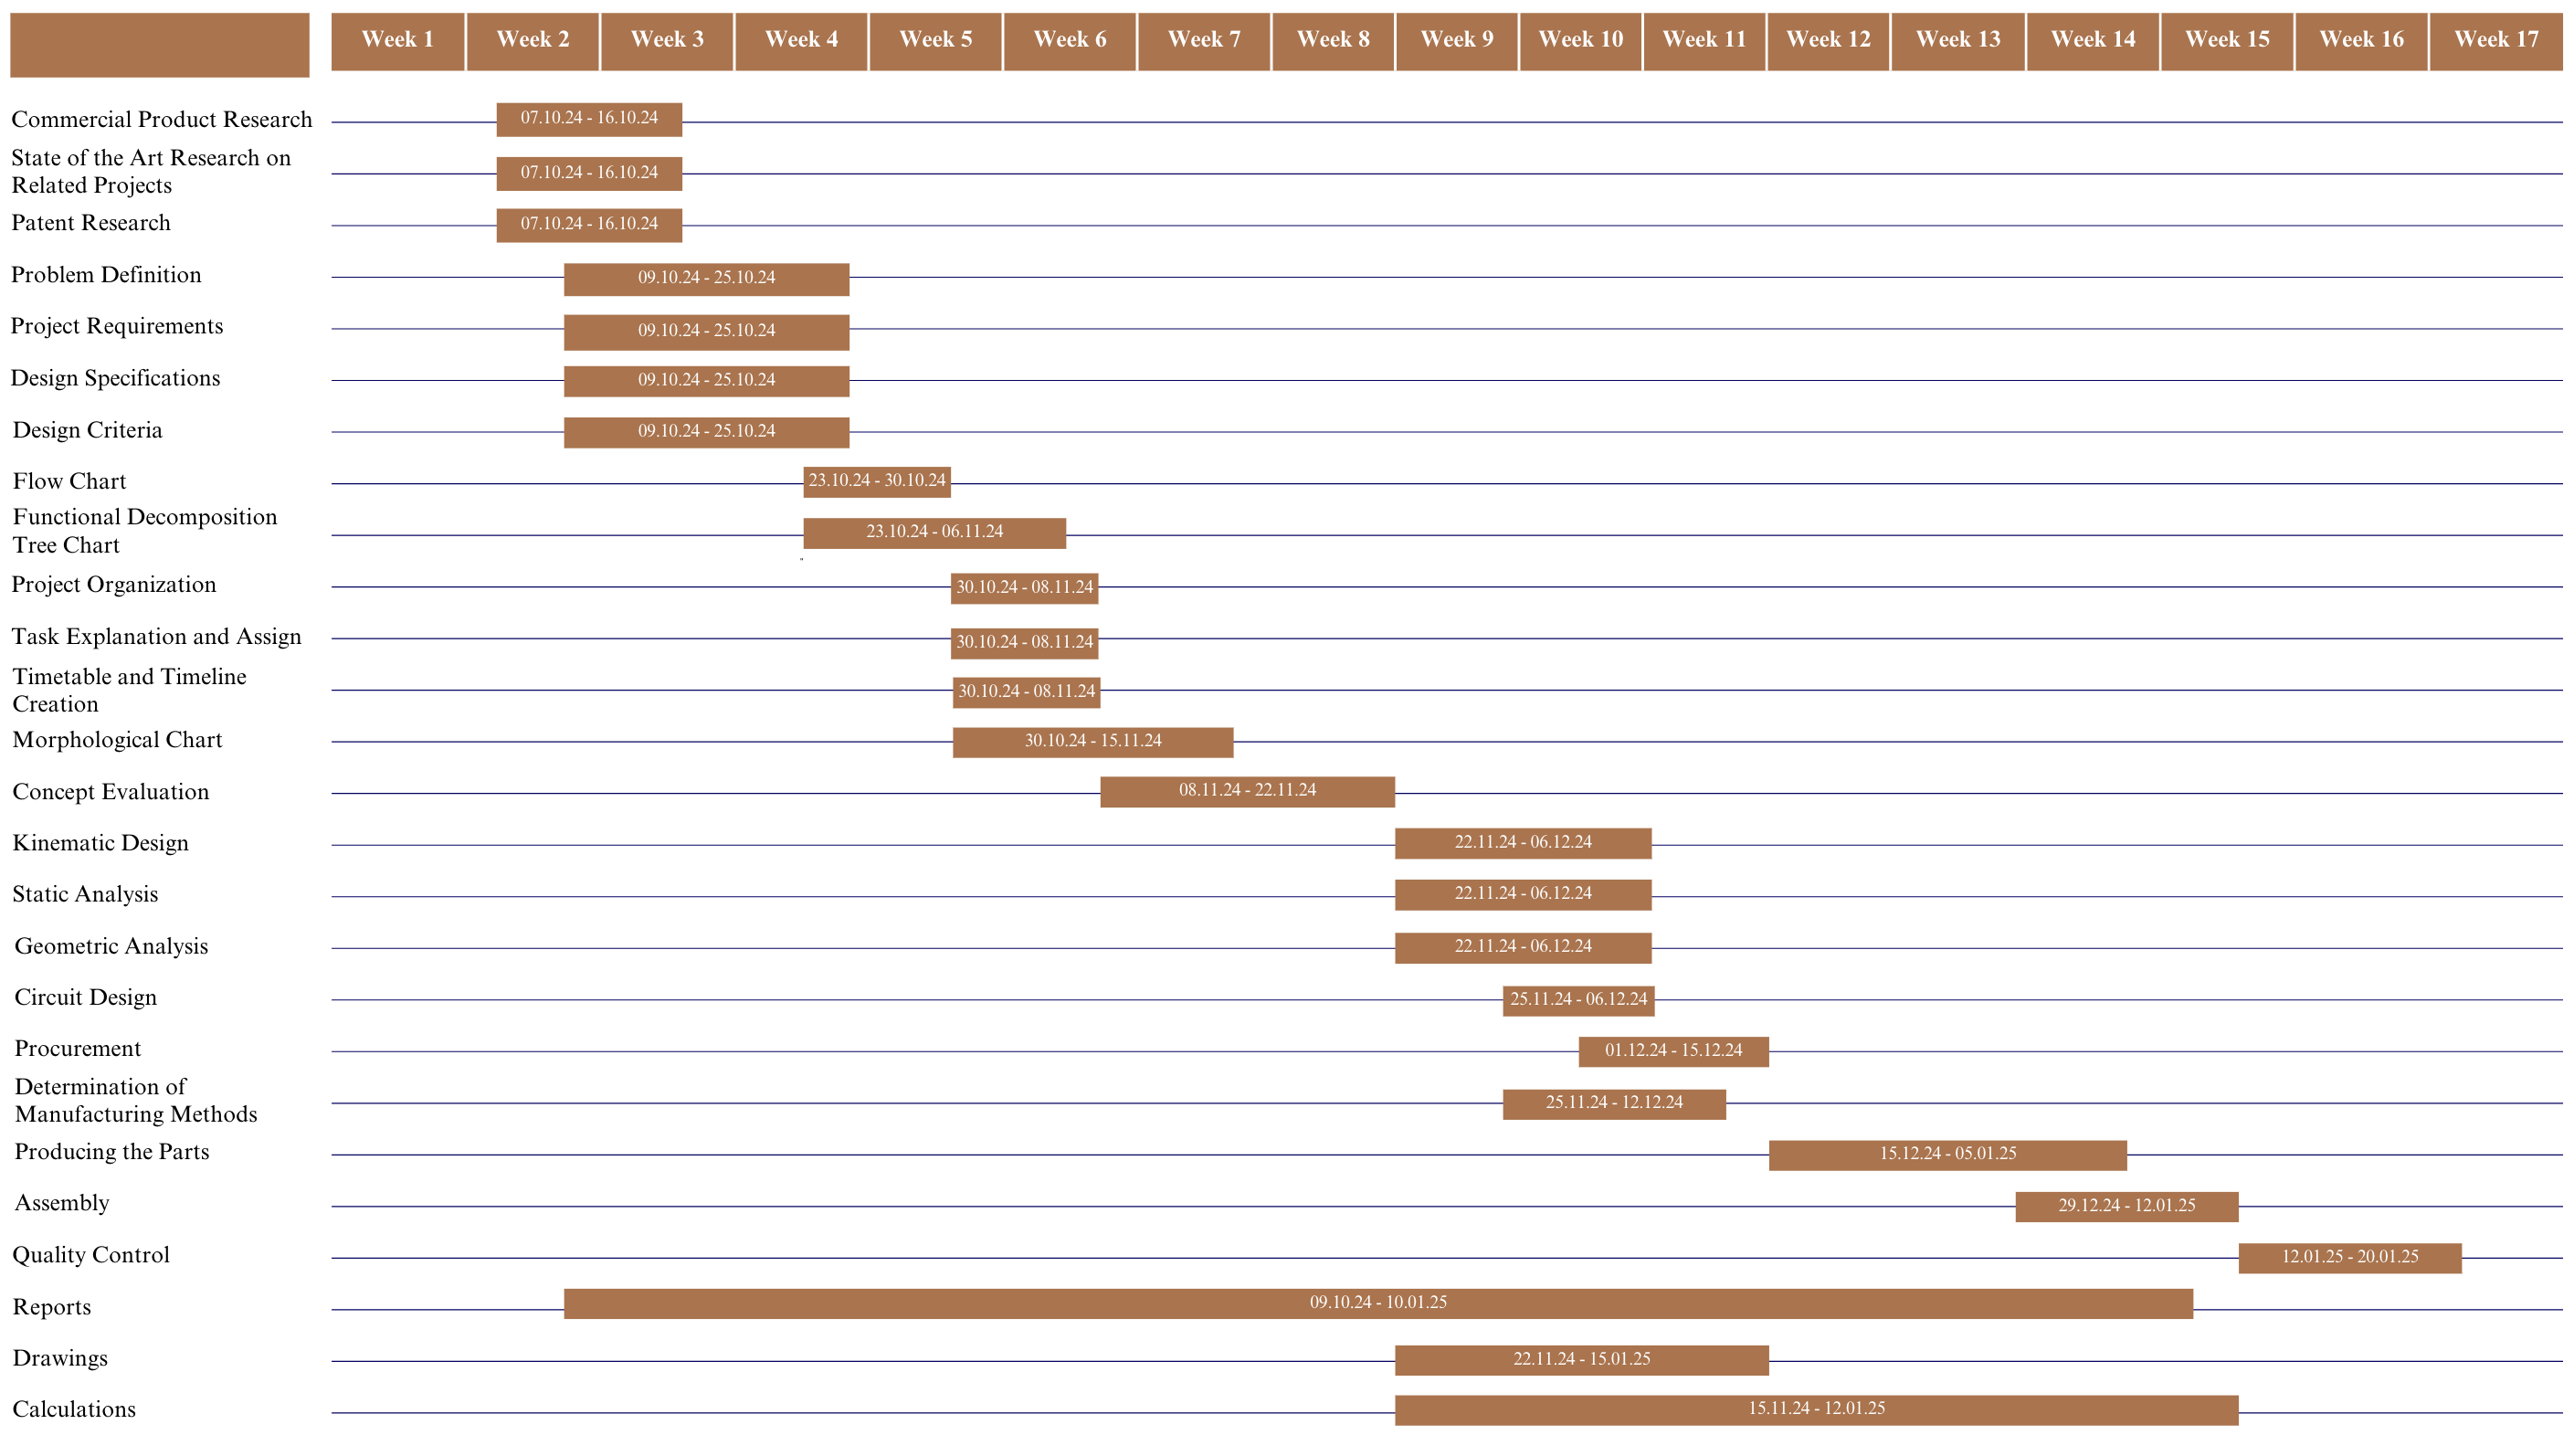
\includegraphics[angle=90, width=\linewidth, height=1.5\linewidth]{Ekran Resmi 2024-11-15 20.07.48.png}
    \caption{Gantt Chart}
    \label{fig:gannt}
\end{figure}

\chapter{Conceptual Design}

\section{Introduction}

This report presents and details the conceptual design part for the project of a Table Tennis Ball Pitcher Machine. By guide of the functional decomposition chart, project requirements and design criteria, and using the function alternatives developed in the morphological chart, different concepts are generated. These concepts are then evaluated in order by the evaluation criteria, and the best concept is chosen to meet the requirements and carry out all functions in the most efficient and effective way.

\section{Concept Development and Presentation}

Concept development and presentation are about turning ideas into clear plans and sharing them effectively. Concept development involves brainstorming, researching, and improving ideas to make them practical. Presentation is about explaining these ideas clearly using stories, visuals, and persuasive communication. Together, they help bring creative ideas to life and make them useful and understandable.

The list form and chart form of the functional decomposition we created during the concept development phase are given below (Fig. \ref{fig:fd}).

\begin{itemize}
    \item Launching the Balls to Desired Places
    \begin{itemize}
        \item Throwing the balls with a desired spin:
        \begin{itemize}
            \item Giving spin to the ball
            \item Controlling the spin
        \end{itemize}
        \item Throwing the balls with a desired speed:
        \begin{itemize}
            \item Giving speed to the ball
            \item Controlling the speed
        \end{itemize}
        \item Throwing the balls with a desired yaw angle:
        \begin{itemize}
            \item Giving yaw angle to the launching mechanism
            \item Controlling the yaw angle
        \end{itemize}
        \item Throwing the balls with a desired pitch angle:
        \begin{itemize}
            \item Giving pitch angle to the launching mechanism
            \item Controlling the pitch angle
        \end{itemize}
    \end{itemize}

    \item Accepting User Inputs
    \begin{itemize}
        \item Accepting frequency information from the user
        \item Accepting trajectory information from the user
        \item Accepting numerical information from the user
        \item Allowing user to position the device
    \end{itemize}

    \item Managing the Supply of the Balls
    \begin{itemize}
        \item Preventing balls from escaping
        \item Storing the balls
        \item Feeding the balls from storage:
        \begin{itemize}
            \item Transferring the balls from storage
            \item Controlling the ball feed from storage
        \end{itemize}
        \item Feeding to launching:
        \begin{itemize}
            \item Transferring the balls to launch
            \item Controlling the ball feed for launching
        \end{itemize}
        \item Managing the frequency of the ball supply:
        \begin{itemize}
            \item Giving the balls the desired frequency
            \item Controlling the ball frequency
        \end{itemize}
    \end{itemize}
\end{itemize}

\begin{figure}[H]
    \centering
    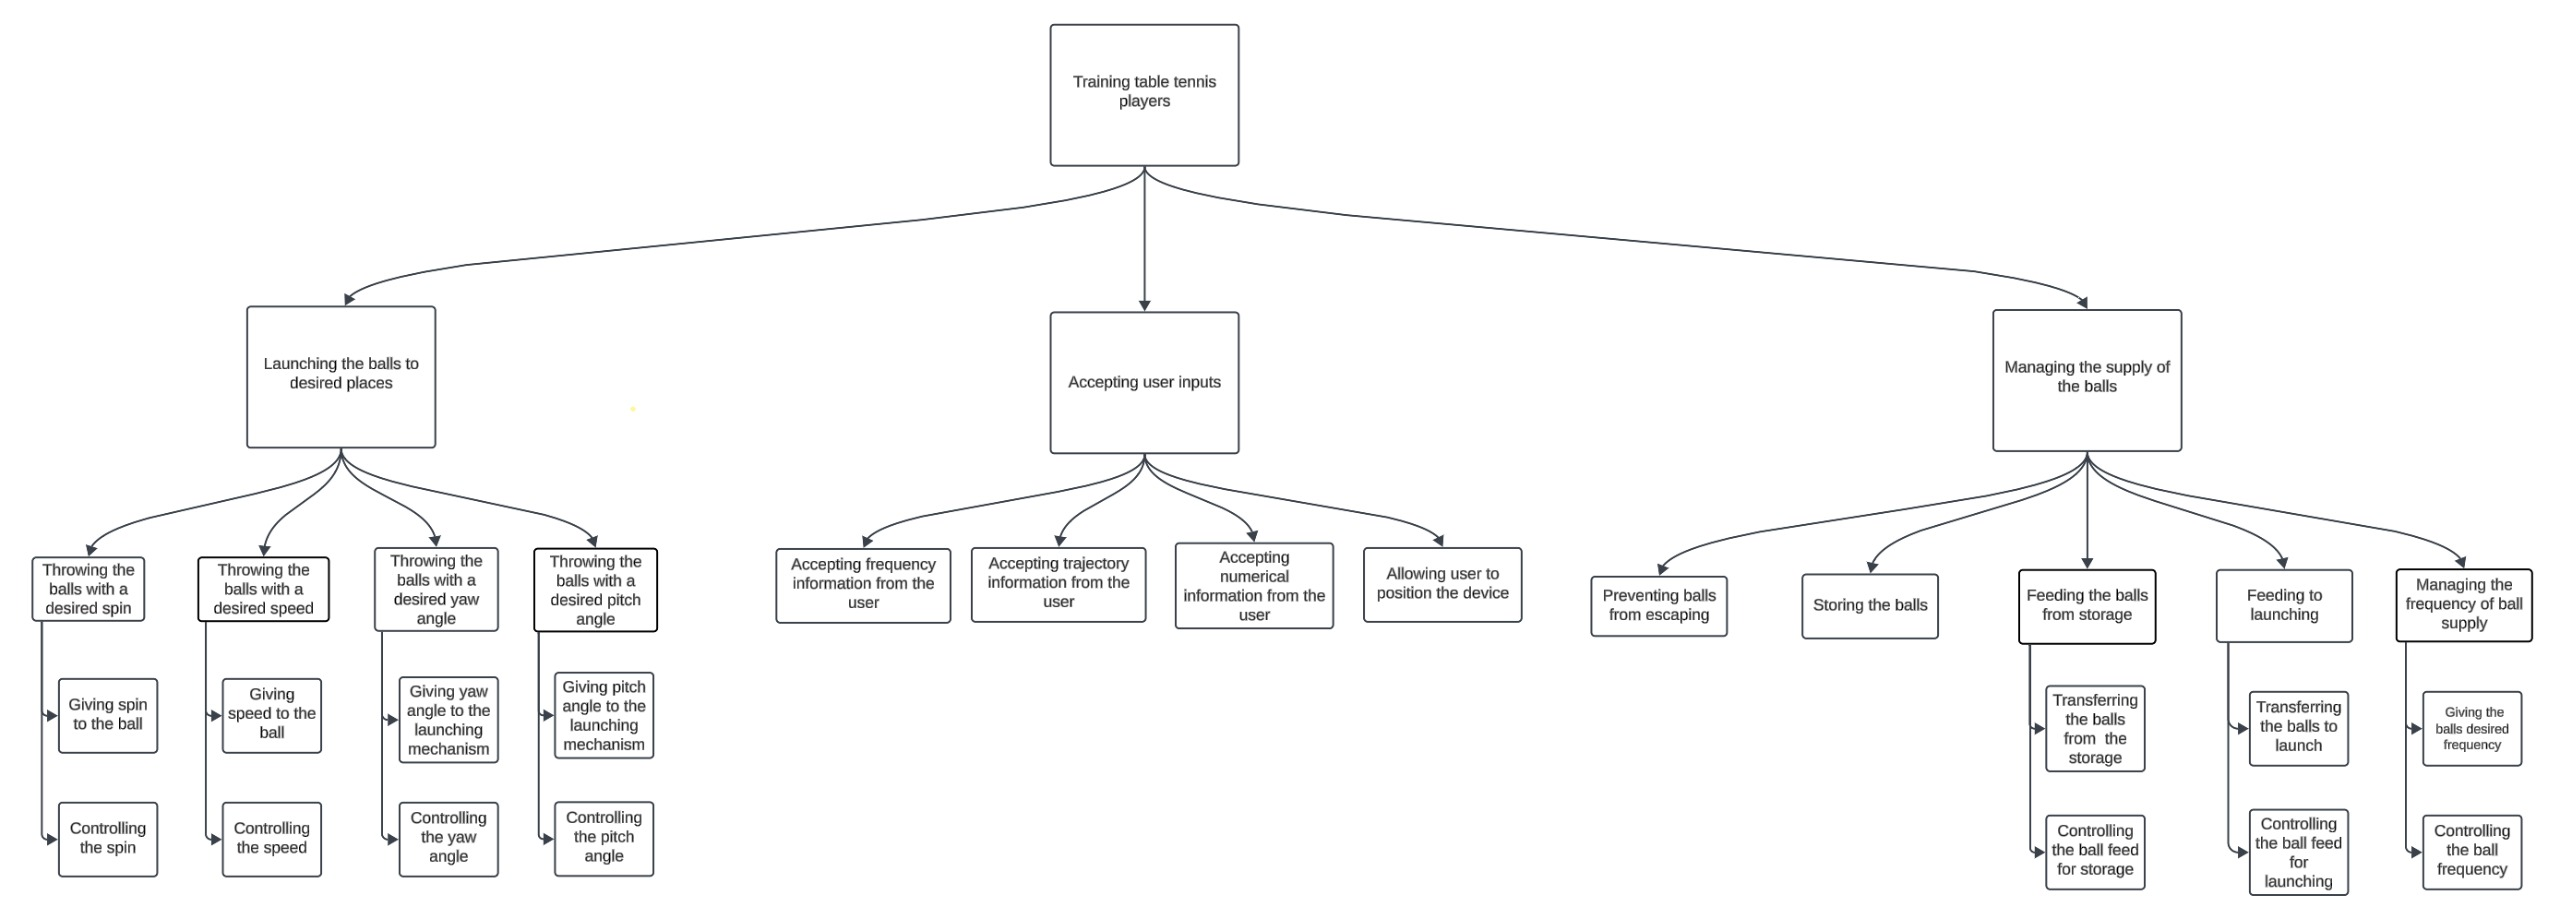
\includegraphics[width=0.9\linewidth]{fd.jpeg}
    \caption{Functional Decomposition}
    \label{fig:fd}
\end{figure}

The morphological chart containing the solutions of the functions included in functional decomposition is located in the Appendix \ref{app:morpho}. \\

The detailed explanation of each concepts are given below: \\

    
    \textbf{Concept 1:}
    
    The balls are to be stored by using a groove mechanism (as shown in Figure ~\ref{fig:groove_mechanism}) while providing recyclability of the balls with a net (Figure ~\ref{fig:net} ). Then the balls are transferred from the storage by a vertical spiral mechanism (Figure ~\ref{fig:spiral}) dictated with a stepper motor. A rotating pusher (Figure ~\ref{fig:rotating_pusher}) at the end of the vertical spiral mechanism is used to direct the balls coming from the spiral to the launching mechanism with desired frequency. The 3 wheel mechanism (Figure ~\ref{fig:3wheel}), which is controlled by DC motors is benefitted to give and control the spin options and speed of the balls. The yaw angle value is controlled by using gears (Figure ~\ref{fig:gear1}), which rotates the head. The pitch angle is controlled by a four bar mechanism (Figure ~\ref{fig:fourbar}). Both controlling mechanisms are connected with servo motors to rotate the head in the desired directions. The trajectory and frequency information are accepted from the user with an integrated controller (Figure ~\ref{fig:integrated}). Accepting numerical information from the user is provided by using a potentiometer with buttons (Figure ~\ref{fig:pot}). Finally, the user is allowed to fix the device to the table by using clamps (Figure ~\ref{fig:clamp}). \\

    \textbf{Concept 2:}
    
    The balls are to be stored by using a box (Figure ~\ref{fig:box}), while providing recyclability of the balls with a net (Figure ~\ref{fig:net}). Then the balls are transferred from the storage to the launcher by a translating box (Figure ~\ref{fig:translating_box}) with a stepper motor. The balls are transferred to launch by the effect of gravity (represented at Figure ~\ref{fig:gravity}), while the desired frequency is provided by a rotating hole (Figure ~\ref{fig:rotating_hole}). The orientation of the hole determines the frequency. The 4 wheel mechanism (Figure ~\ref{fig:4wheel}), which is controlled by BLDC motors is benefitted to give and control the spin options and speed of the balls. The yaw angle values are controlled by using four bar mechanisms (Figure ~\ref{fig:fourbar_yaw}), and pitch angle values are controlled by a rope controlled head pulley (Figure ~\ref{fig:rope})  to rotate the head in the desired directions. Both mechanisms are dictated by servomotors. The trajectory and frequency information are accepted from the user with an integrated controller (Figure ~\ref{fig:integrated}). Accepting numerical information from the user is provided by using a potentiometer with buttons (~\ref{fig:pot}). Finally, the user is allowed to fix the device to the table by using clamps (Figure ~\ref{fig:clamp}). \\

    \textbf{Concept 3:}

    The balls are to be stored by using a box (Figure ~\ref{fig:box}) while providing recyclability of the balls with a net (Figure ~\ref{fig:net}). Then the balls are transferred from the storage to the launcher by a vertical spiral mechanism (shown at Figure ~\ref{fig:spiral}) dictated with a stepper motor. A rotating pusher (Figure ~\ref{fig:rotating_pusher}) at the end of the vertical spiral mechanism is used to direct the balls coming from the spiral to the launching mechanism and give the desired launch frequency. The 2 wheel mechanism (Figure ~\ref{fig:2wheel}), which is controlled by DC motors is benefitted to give and control the spin options and speed of the balls. The control of yaw and pitch angle is provided by bevel gear mechanisms (Figures ~\ref{fig:bevel} and ~\ref{fig:bevel_yaw}). Both controlling mechanisms are connected with servo motors to rotate the head in the desired directions. The trajectory and frequency information are accepted from the user with a wired remote (Figure ~\ref{fig:wired}). Accepting numerical information from the user is provided by using a potentiometer with buttons (Figure ~\ref{fig:pot}). Finally, the user is allowed to fix the device to the table by using a clamp mechanism (Figure ~\ref{fig:clamp}). \\

    \textbf{Concept 4:}

    The balls are to be stored by using a groove mechanism (Figure ~\ref{fig:groove_mechanism}) while providing recyclability of the balls with a net (Figure ~\ref{fig:net}). Then the balls are transferred from the storage to the launcher by a maltese wheel mechanism (Figure ~\ref{fig:maltese}) dictated with a stepper motor. Also, this maltese wheel is used to direct the balls to the launching mechanism by the pushing effect of the consecutive balls and helps give the desired frequency. The 3 wheel mechanism (Figure ~\ref{fig:3wheel}), which is controlled by BLDC motors is benefitted to give and control the spin options and speed of the balls. The control of yaw and pitch angle values are done by gear mechanisms (Figures ~\ref{fig:gear} and ~\ref{fig:gear2}), which are connected with servo motors. The gears control the pitch and yaw angle values by rotating the head and base, respectively. The trajectory and frequency information are accepted from the user with an integrated controller (Figure ~\ref{fig:integrated}). Accepting numerical information from the user is provided by using a potentiometer with buttons (Figure ~\ref{fig:pot}). Finally, the user is allowed to fix the device to the table by using clamps (Figure ~\ref{fig:clamp}). \\

    \textbf{Concept 5:}

    The balls are to be stored by using a tunnel mechanism (Figure ~\ref{fig:tunnel_mechanism}) while providing recyclability of the balls with a net (Figure ~\ref{fig:net}). This tunnel is placed between a maltese wheel (Figure ~\ref{fig:maltese}) on bottom and a slider crank (Figure ~\ref{fig:slider_crank}) at top, the maltese wheel enables the ball entrance to the tunnel from the net, whereas the slider crank transfers balls to the launching with desired frequency. These maltese wheels are activated with stepper motors. The 2 tension belt with spinning head mechanism (Figure ~\ref{fig:2tension}), which is controlled by BLDC motors is benefitted to give and control the spin options and speed of the balls. The control of pitch angle is provided by a worm gear mechanism (Figure ~\ref{fig:worm}) and the yaw angle is controlled by a gear mechanism (Figure ~\ref{fig:gear2}), rotating the head from the base. Both controlling mechanisms are connected with servo motors to rotate the head in the desired directions. The trajectory and frequency information are accepted from the user with an integrated controller (Figure ~\ref{fig:integrated}). Accepting numerical information from the user is provided by using an encoder (Figure ~\ref{fig:encoder}) . Finally, the user is allowed to fix the device to the table by using clamps (Figure ~\ref{fig:clamp}). \\

    \textbf{Concept 6:}

    The balls are to be stored by using a groove mechanism (Figure ~\ref{fig:groove_mechanism}) while providing recyclability of the balls with a net (Figure ~\ref{fig:net}). A maltese wheel (Figure ~\ref{fig:maltese}) is benefitted to raise the balls to a selected elevation and the transferring process from the storage is initiated. Then the balls are transferred to the launcher by the effect of gravity (represented at Figure ~\ref{fig:gravity}) . The desired frequency is given by the movement of a lid mechanism (Figure ~\ref{fig:lid_mechanism}). The 3 wheel mechanism (Figure ~\ref{fig:3wheel}) , which is controlled by DC motors is benefitted to give and control the spin options and speed of the balls. The control of yaw and the pitch angle is controlled by four bar mechanisms (Figures ~\ref{fig:fourbar_yaw} and ~\ref{fig:fourbar}). Both controlling mechanisms are connected with servo motors to rotate the head in the desired directions. The trajectory and frequency information are accepted from the user with an integrated controller (Figure ~\ref{fig:integrated}). Accepting numerical information from the user is provided by using a potentiometer with buttons (Figure ~\ref{fig:pot}). Finally, the user is allowed to fix the device to the table by using clamps (Figure ~\ref{fig:clamp}). \\

    \textbf{Concept 7:}

    The balls are to be stored by using a groove mechanism (Figure ~\ref{fig:groove_mechanism}) while providing recyclability of the balls with a net (Figure ~\ref{fig:net}). Then the balls are transferred from the storage to the launcher by a belt mechanism (Figure ~\ref{fig:belt}) dictated with a stepper motor. A maltese wheel (Figure ~\ref{fig:maltese_wheel} ) mechanism is used to direct the balls coming from the vertical belt to the launching mechanism, also the desired frequency is given. The 2 wheel mechanism (Figure ~\ref{fig:2wheel}), which is controlled by BLDC motors is benefitted to give and control the spin options and speed of the balls. The pitch angle value is controlled by using bevel gear (Figure ~\ref{fig:bevel}), and yaw angle value is controlled by a worm gear (Figure ~\ref{fig:worm_yaw}). Both controlling mechanisms are connected with servo motors to rotate the head in the desired directions. The trajectory and frequency information are accepted from the user with an integrated controller (Figure ~\ref{fig:integrated}). Accepting numerical information from the user is provided by using a potentiometer with buttons (Figure ~\ref{fig:pot}). Finally, the user is allowed to fix the device to the table by using clamps (Figure ~\ref{fig:clamp} ). \\



    \textbf{Concept 8:}

    The balls are to be stored by using a groove mechanism (Figure ~\ref{fig:groove_mechanism}) while providing recyclability of the balls with a net (Figure ~\ref{fig:net}). Then the balls are transferred from the storage to a vertical tube by a maltese wheel (Figure ~\ref{fig:maltese}) dictated with a stepper motor. The end of the tube is at a higher elevation from the launch. The balls are released from the tip to the launching mechanism. The gravitational force (represented at Figure ~\ref{fig:gravity}) provides the transfer to launch. The required frequency is set by a hinge mechanism (Figure ~\ref{fig:hinge_mechanism}), the movement of the hinge mechanism determines the frequency. The 4 wheel mechanism (Figure ~\ref{fig:4wheel}), which is controlled by BLDC motors is benefited to give and control the spin options and speed of the balls. The pitch angle value is controlled by using a four bar mechanism (Figure ~\ref{fig:fourbar}), and yaw angle value is controlled by a gear, which rotates the head (Figure ~\ref{fig:gear2}) . Both controlling mechanisms are connected with servo motors to rotate the head in the desired directions. The trajectory and frequency information are accepted from the user with an integrated controller (Figure ~\ref{fig:integrated}). Accepting numerical information from the user is provided by using an encoder (Figure ~\ref{fig:encoder}). Finally, the user is allowed to fix the device to the table by using clamps (Figure ~\ref{fig:clamp}). \\
  

\section{Evaluation of Concepts}

The evaluation of criteria was conducted using the Analytic Hierarchy Process (AHP) method. Initially, Saaty's Fundamental scale for pairwise comparison is utilized. This method employs a pairwise comparison approach, which means that each criterion is compared to every other criterion on Saaty's 1-9 scale of relative importance. This scale goes from 1 (equal importance) to 9 (absolute importance), with intermediate values (2, 4, 6, 8) denoting nuanced assessments. Then these values were normalized, and weighted averages were calculated to ensure a consistent and unbiased evaluation framework. \\

In addition to assessing each concept, the evaluation criteria were also applied to analyze the functions and corresponding solutions presented in the morphological chart. For each function, a decision matrix was constructed, and the solution with the highest score in each matrix was identified as the optimal choice for that specific function. This systematic approach ensured that both the overall concepts and individual functions were evaluated objectively.


Our design criteria are as follows:


\begin{enumerate}
    \item \textbf{Serving Frequency:} Can throw 80 balls per minute and more. Also, adjustable within 25-80 balls per minute.
    \item \textbf{Feeding the Ball}: Allows for uninterrupted training with desired frequency.
    \item \textbf{Serving Speed:} Adjustable between 4 m/s and 25 m/s. Can throw balls at 25 m/s and more.
    \item \textbf{Preventing Balls from Escaping:} The design can collect balls that came up to 1 meter height on its side.
    \item \textbf{Selectable Serving Modes:} Supports various training modes.
    \item \textbf{Giving Yaw and Pitch Angle:} Angles need to be adjustable within specified ranges accurately.
    \item \textbf{Portability:} Less than the maximum weight which is 15 kg, easy to set up.
    \item \textbf{Capacity:} Minimum storage of 100 balls.
    \item \textbf{Ball Durability:} Balls should withstand at least 1000 throws.
    \item \textbf{Power Consumption:} Energy efficiency is prioritized.
    \item \textbf{Spin Options:} Ability to generate 36 spins for varied training.
    \item \textbf{User Interface:} It should be easy to use and should not contain complicated buttons.
    \item \textbf{Cost:} The design should be cost efficient, the cost of manufacturing must be less than 300 dolars.
    \item \textbf{No Spin (Bonus):} Throwing should be possible without spin.
    \item \textbf{Different Scenarios (Bonus):} Allow different types of throws, for example starting with a serve.
\end{enumerate}


Based on the design criteria, the evaluation criteria are derived as follows:
\begin{enumerate}
    \item \textbf{Maximum Attainable Serving Frequency:} The highest number of balls the machine can serve per second. Measures the machine's overall capability to serve balls at its highest possible rate, regardless of how the balls are fed. This criterion is derived from the "Serving Frequency" design criterion, as achieving a high maximum frequency ensures the machine can meet a wide range of performance requirements with flexibility for lower frequencies.

    \item \textbf{Serving Frequency Adjustment Accuracy:} The precision of frequency adjustment, measured as deviation from the target frequency. This criterion is also derived from "Serving Frequency," focusing on how accurately the machine can meet specific serving rates, crucial for scenarios that require controlled and consistent ball delivery.

    \item \textbf{Maximum Feeding Speed:} The rate at which the machine loads and serves balls from the reservoir, ensuring continuous and efficient operation without interruptions. Focuses specifically on the efficiency of the feeding mechanism to supply balls into the serving system at a consistent rate. This criterion is derived from the "Feeding the Balls" design criterion, as the ability to achieve a high feeding speed ensures the machine can handle demanding use cases while maintaining a smooth and consistent supply of balls to the serving mechanism.

    \item \textbf{Maximum Attainable Pitch and Yaw Angle:} The highest vertical and horizontal angle the machine can achieve, determining its capability to simulate lobs or high-arc serves and allowing it to target various positions across the table for diverse shot placement. This criterion is derived from the "Giving Yaw and Pitch Angle" design criterion, as evaluating the maximum angles ensures the machine can cover a wide range of shot trajectories and placements, providing versatility and precision in gameplay scenarios.


    \item \textbf{Ball Prevention Efficiency:} The proportion of prevented balls from escaping successfully and transferred to the reservoir. This criterion is derived from the "Preventing Balls from Escaping" design criterion, as it quantifies the effectiveness of the mechanism in retaining balls, ensuring minimal loss during operation and maintaining a consistent supply for serving.

    \item \textbf{Serving Accuracy:} Average deviation of the ball's landing point from the target. This criterion is derived from "Giving Yaw and Pitch Angle," "Serving Speed," and "Feeding the Balls" design criteria, as accurate targeting requires precise control over ball direction, velocity, and feeding consistency. Additionally, it depends on the "Serving Frequency" design criterion to ensure that accuracy is maintained even at the desired serving rates.  


    \item \textbf{Serving Precision:} Consistency of serving, measured as the standard deviation of ball landing points. This criterion is derived from "Giving Yaw and Pitch Angle," "Serving Speed," and "Feeding the Balls" design criteria, as consistent ball placement relies on stable directional control, speed regulation, and feeding. The "Serving Frequency" design criterion also plays a role by ensuring precision is upheld across various serving rates without performance degradation.


    \item \textbf{Maximum Attainable Serving Speed:} The fastest ball velocity the machine can achieve. This criterion is derived from "Feeding the Balls" and "Serving Speed" design criteria, as achieving high serving speeds requires efficient feeding of balls into the serving mechanism and robust control over the velocity imparted to the ball during the serving process.


    \item \textbf{Portability:} Subjective score based on factors such as weight, size, and transportability. This criterion is derived from the "Portability" design criterion, as it assesses how easy it is to move, transport, and store the machine, taking into account the overall design and physical characteristics that influence its mobility.

    \item \textbf{Reservoir Capacity:} Maximum number of balls the reservoir can hold. This criterion is derived from the "Capacity" design criterion, as it measures the machine's ability to store and supply a sufficient number of balls for uninterrupted operation, impacting both performance and convenience during extended use.

    \item \textbf{Ball Durability:} Percentage of wear or deformation observed on balls after a specified number of serves. This criterion is derived from the "Capacity" design criterion, as the ability to store and serve a large number of balls without causing excessive wear or damage directly impacts the longevity and performance of the balls over time.

    \item \textbf{Energy Consumption:} Average power usage during operation. This criterion is derived from the "Power Consumption" design criterion, as it measures the efficiency of the machine in terms of energy usage, reflecting how well the system optimizes power consumption during its operation.

    \item \textbf{Spin Options Variety:} Number of spin types the machine can generate (e.g., topspin, backspin, sidespin). This criterion is derived from the "Spin Options" design criterion, as it evaluates the variety of spin types the machine can produce, which directly affects the range of gameplay scenarios it can simulate.

    \item \textbf{Cost:} Total cost of manufacturing or purchasing the machine. This criterion is derived from the "Cost" design criterion, as it directly reflects the financial aspect of producing or acquiring the machine, factoring in materials, labor, and other associated expenses.

    \item \textbf{Ease of Manufacturing:} A subjective score reflecting the ease or difficulty of manufacturing the machine. This criterion is derived from all the design criteria, as the complexity of the overall design, including components like feeding mechanisms, serving accuracy, spin options, and portability, directly influences how easy or difficult it is to manufacture the machine.

    \item \textbf{Response Time:} The time the system takes to reach its target value after a command, indicating its speed and efficiency. This criterion is derived from "Serving Speed" and "Giving Yaw and Pitch Angle" design criteria, as the ability to quickly adjust the serving speed and angles directly affects how fast the machine can respond to commands and achieve the desired target values.


    \item \textbf{User Friendliness:} Focuses on the clarity of the controls, the simplicity of the process, and how quickly a user can achieve desired outcomes without confusion or excessive effort. This criterion is derived from the "User Interface" design criterion, as the design and layout of the interface directly influence how intuitive and straightforward the machine is for users to operate and achieve their desired settings.


    \item \textbf{Ease of Control:} Evaluates how straightforward and intuitive it is to manage, adjust, or optimize the system during development and operation, ensuring minimal complexity and effort. This criterion is derived from the overall functions of the machine, as it focuses on the designer's perspective, ensuring that the system’s functions are easily adjustable and controllable to achieve desired outcomes with precision and efficiency.

    \item \textbf{Ease of Mounting:} Measures how quickly and effortlessly the user can mount the device onto the setup. This criterion is derived from the "Portability" design criterion, as a portable design inherently involves considerations for simple and convenient mounting, ensuring that the device can be securely and efficiently attached or detached without requiring excessive effort or specialized tools.


    \item \textbf{Maximum Supplied Speed:} Evaluates the maximum speed that the system’s power source can provide to drive key functions such as serving frequency, feeding mechanisms, and serving speed. This criterion is derived from "Serving Frequency," "Feeding the Balls," and "Serving Speed" design criteria, as it focuses on the capability of the system’s core power source (most likely an electric motor but not restricted to one) to ensure optimal operation of these interconnected functions. It is critical for controlling and enabling the precise and efficient movement of these subsystems.

    
\end{enumerate}

The relative importance of the criteria is evaluated and presented in the matrix shown in Figure~\ref{fig:cvc1}. The normalized version of the evaluated criteria table, along with the derived weighting factors, is depicted in Figure~\ref{fig:cvc2}. These criteria and their corresponding weighting factors are important, as they will be used in selecting the best solution for each subfunction. In the following sections of the report, the weighting factors shown in Figure~\ref{fig:cvc2} will be considered.


\begin{figure}[H]
    \centering
    \rotatebox{90}{\includegraphics[width=\textheight]{cvc1.jpg}}
    \caption{Criteria vs Criteria Evaluation}
    \label{fig:cvc1}
\end{figure}

\begin{figure}[H]
    \centering
    \rotatebox{90}{\includegraphics[width=\textheight]{cvc2.jpg}}
    \caption{Criteria vs Criteria Evaluation Normalized}
    \label{fig:cvc2} 
\end{figure}

This section presents the decision matrices to evaluate the 20 subfunctions of the table tennis ball launcher design. Each subfunction was evaluated using several solution options, which were compared to a set of established evaluation criteria. The relative relevance of these criteria was determined by a pairwise comparison utilizing Saaty's Analytical Hierarchy Process (AHP), which generated weighting factors based on the criterion vs. criterion relative importance matrix. \\

The decision matrices use these weighting factors to identify the best solution for each subfunction. By carefully evaluating and rating each possibility against the criteria, decision matrices give a clear and rational foundation for selecting the best answer for each subfunction.




Five design alternatives were considered for giving spin to the ball. Based on a thorough decision matrix analysis, the three-wheel configuration was identified as the most suitable option as can be seen in Figure~\ref{fig:spin}. This design outperformed the two-wheel system with a rotating head and the four-wheel configuration in terms of efficiency and simplicity. The four-wheel setup posed challenges due to the complexity of synchronizing four independent motors, which could lead to slower response times. Meanwhile, the two-wheel system with a spinning head required additional time to adjust the head's motion to generate the desired spin. Thus, the three-wheel configuration was selected as the optimal solution for imparting spin to the ball.
\begin{figure}[H]
    \centering
    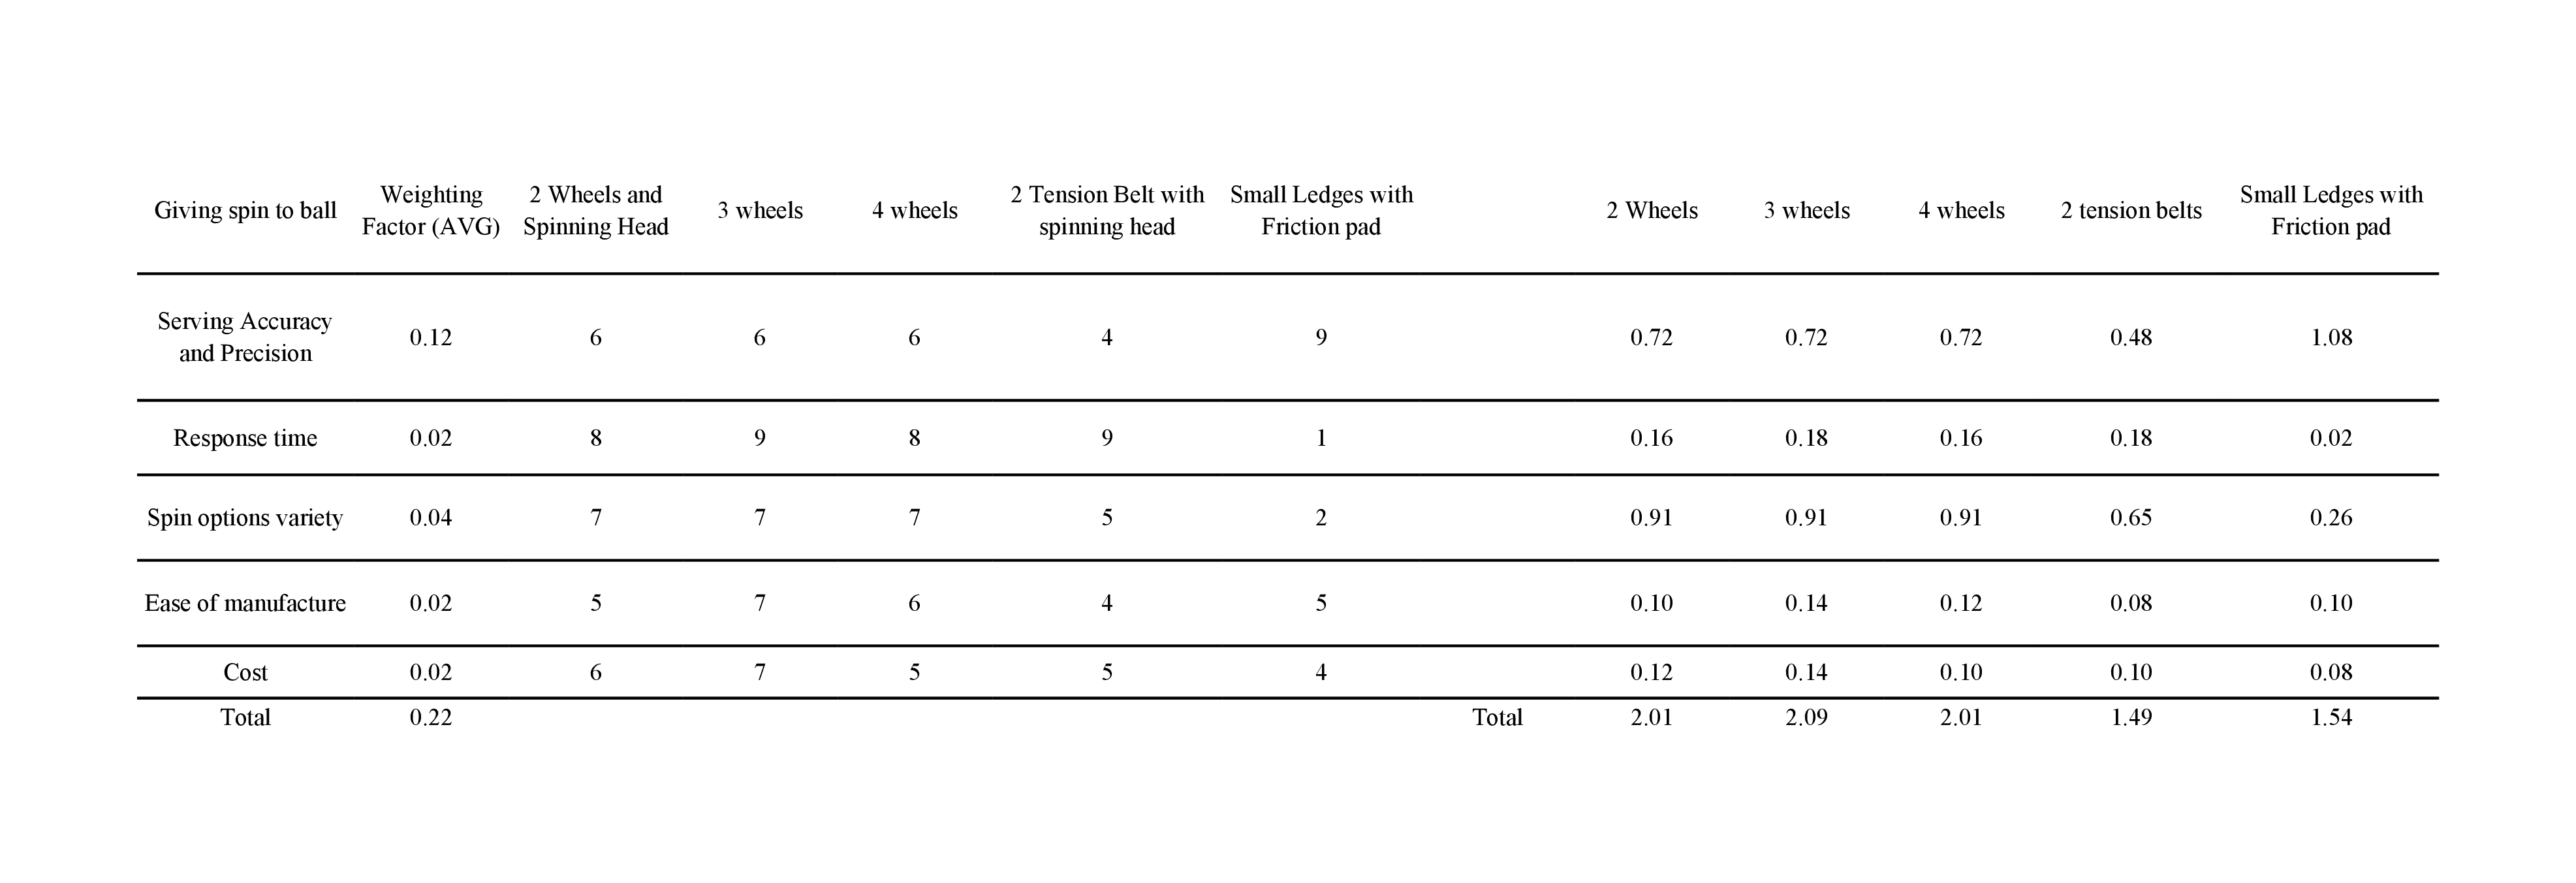
\includegraphics[width=1\textwidth]{Decision matrices/spin.png}
    \caption{Giving spin to the ball}
    \label{fig:spin}
\end{figure}



Three alternatives were considered for controlling spin: DC, BLDC, and stepper motors. Based on the decision matrix evaluation, BLDC motors were selected as the optimal solution. This choice was driven by their better accuracy and precision, as well as their ability to provide a higher maximum supplied speed compared to the other options.
\begin{figure}[H]
    \centering
    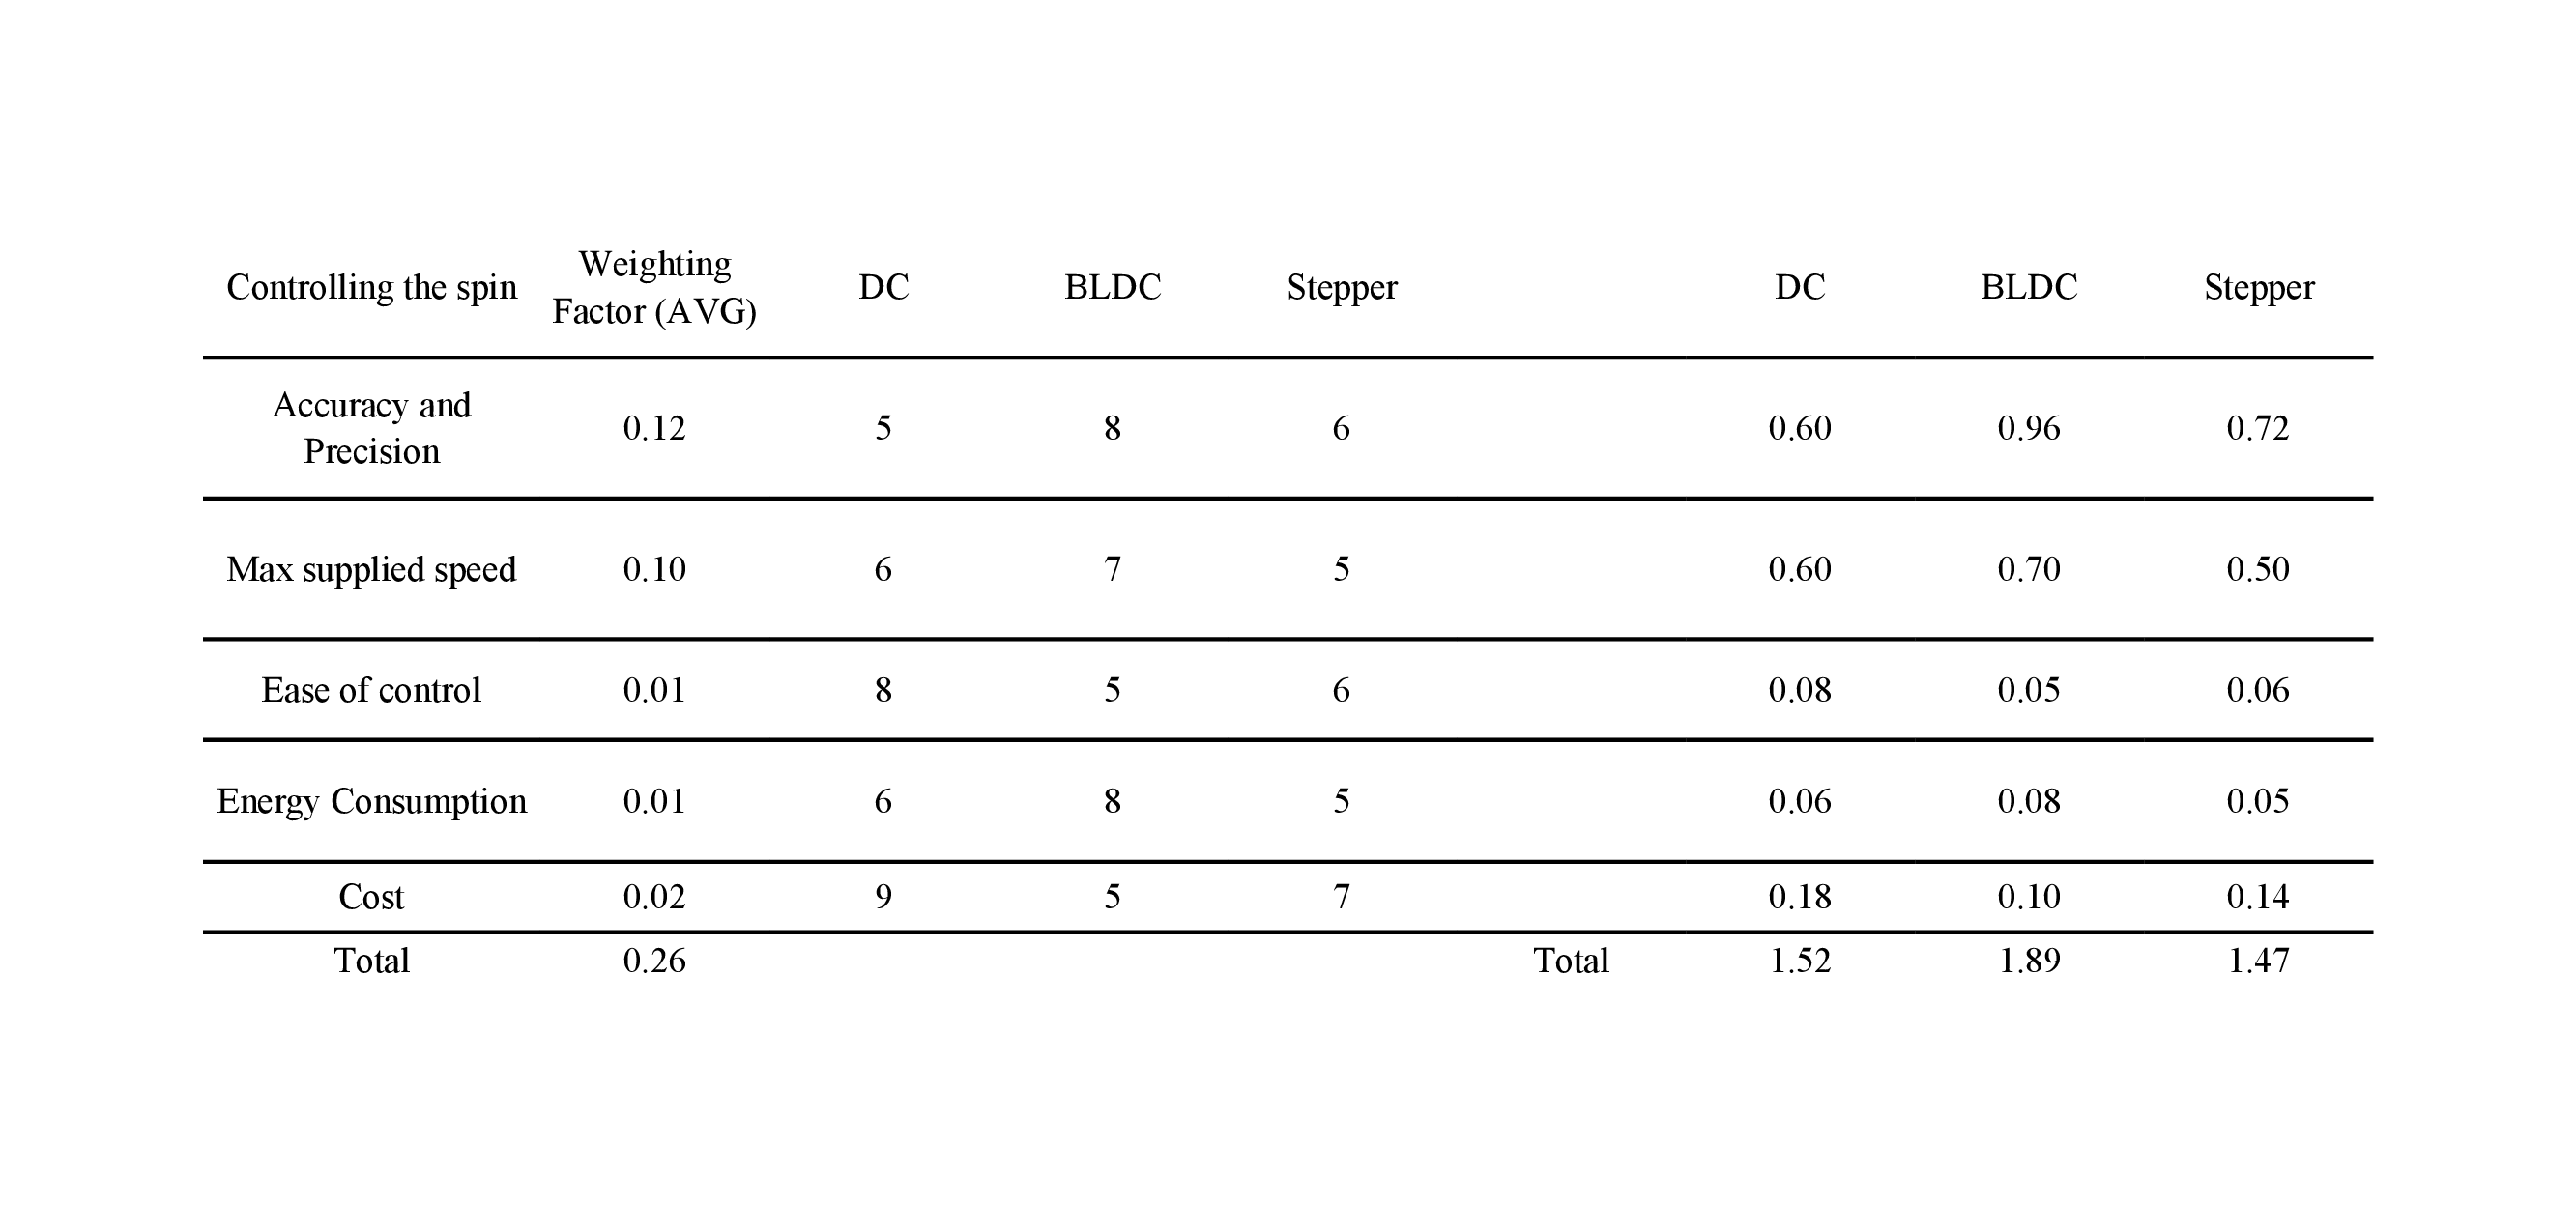
\includegraphics[width=0.8\textwidth]{Decision matrices/controlling spin.png}
    \caption{Controlling the spin}
\end{figure}


Six design alternatives were considered for giving speed to the ball. As with giving spin, the decision matrix evaluation identified the three-wheel configuration as the best alternative. It was also discussed in the context of achieving spin, the three-wheel design demonstrated significant advantages over the two-wheel system with a rotating head and the four-wheel configuration. The four-wheel setup posed challenges due to the complexity of synchronizing four independent motors, potentially increasing response time. Similarly, the two-wheel system with a spinning head required additional time to adjust the head's motion to generate the desired speed. Consequently, the three-wheel configuration was selected as the optimal solution for giving speed to the ball, consistent with its performance in spin application.

\begin{figure}[H]
    \centering
    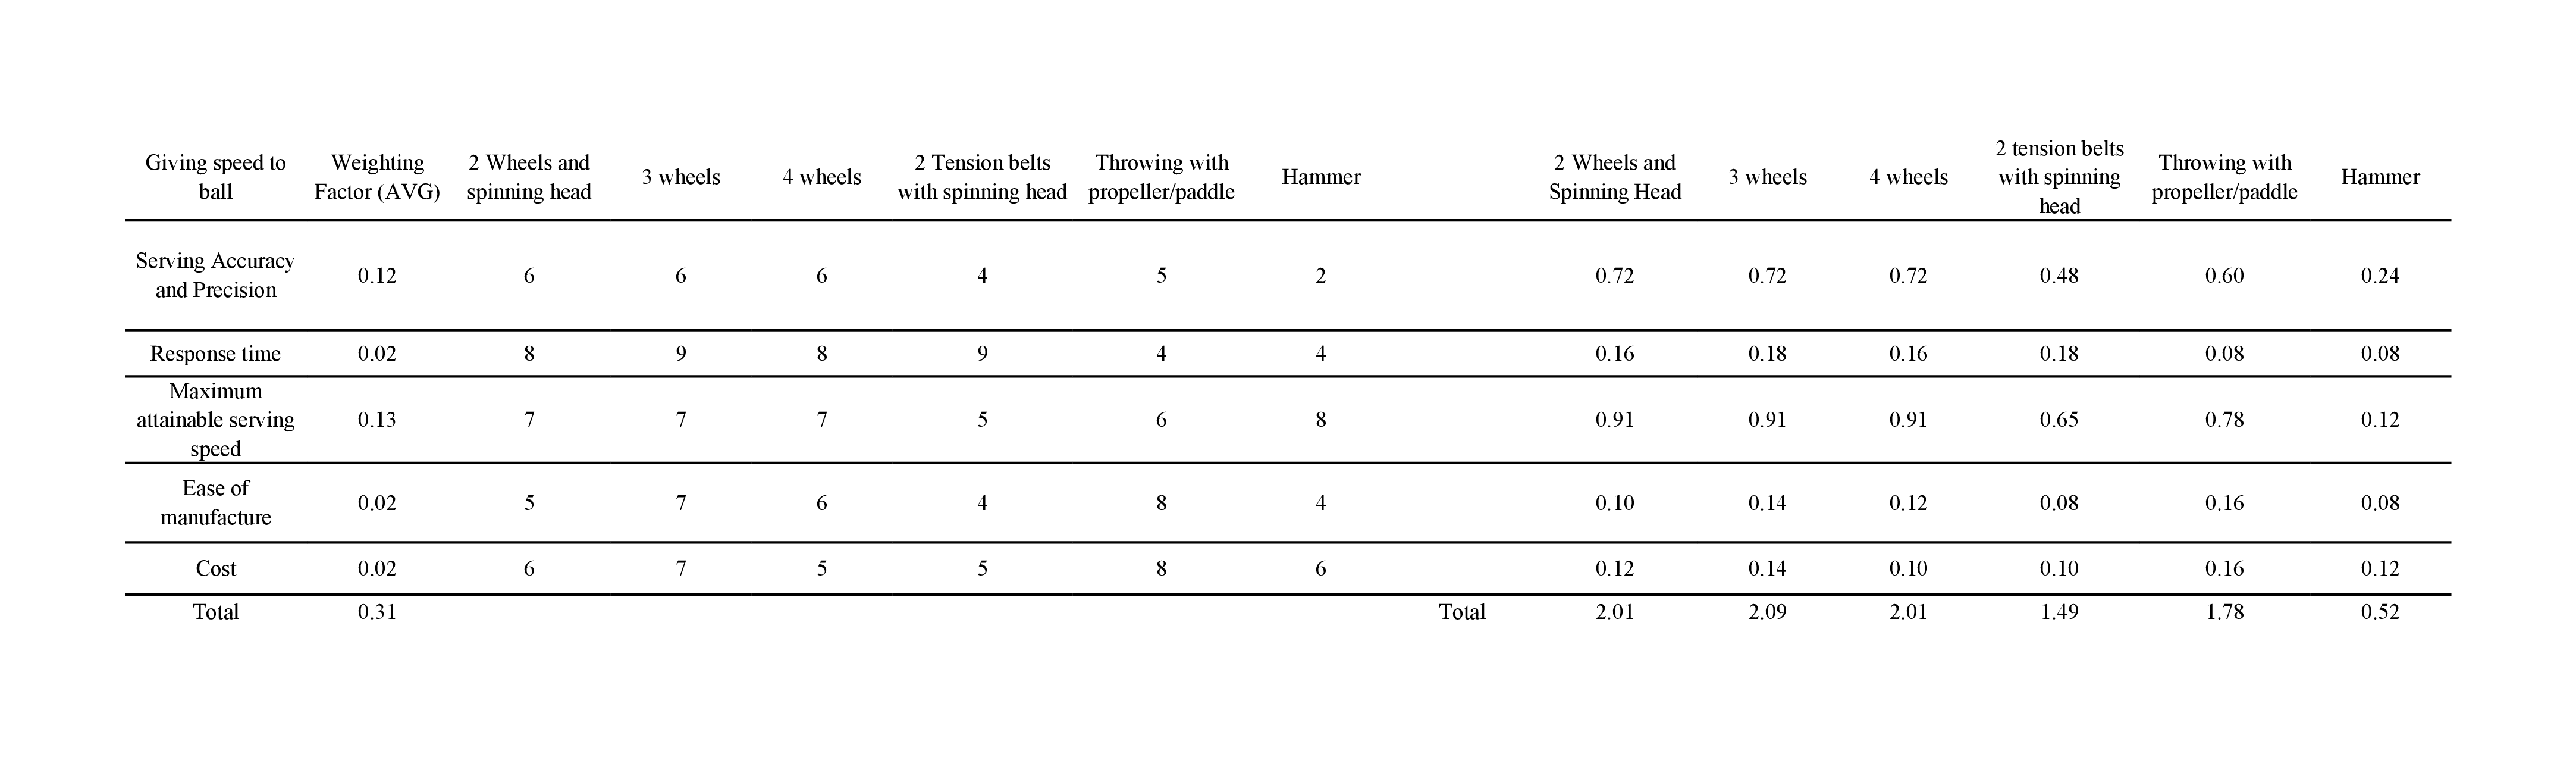
\includegraphics[width=1\textwidth]{Decision matrices/speed.png}
    \caption{Giving speed to the ball}
\end{figure}

Similarly, three alternatives were considered for controlling the speed of the balls. As was the case in controlling spin, BLDC motors were identified as the optimal solution due to their superior accuracy, precision, and ability to deliver higher maximum speeds.
\begin{figure}[H]
    \centering
    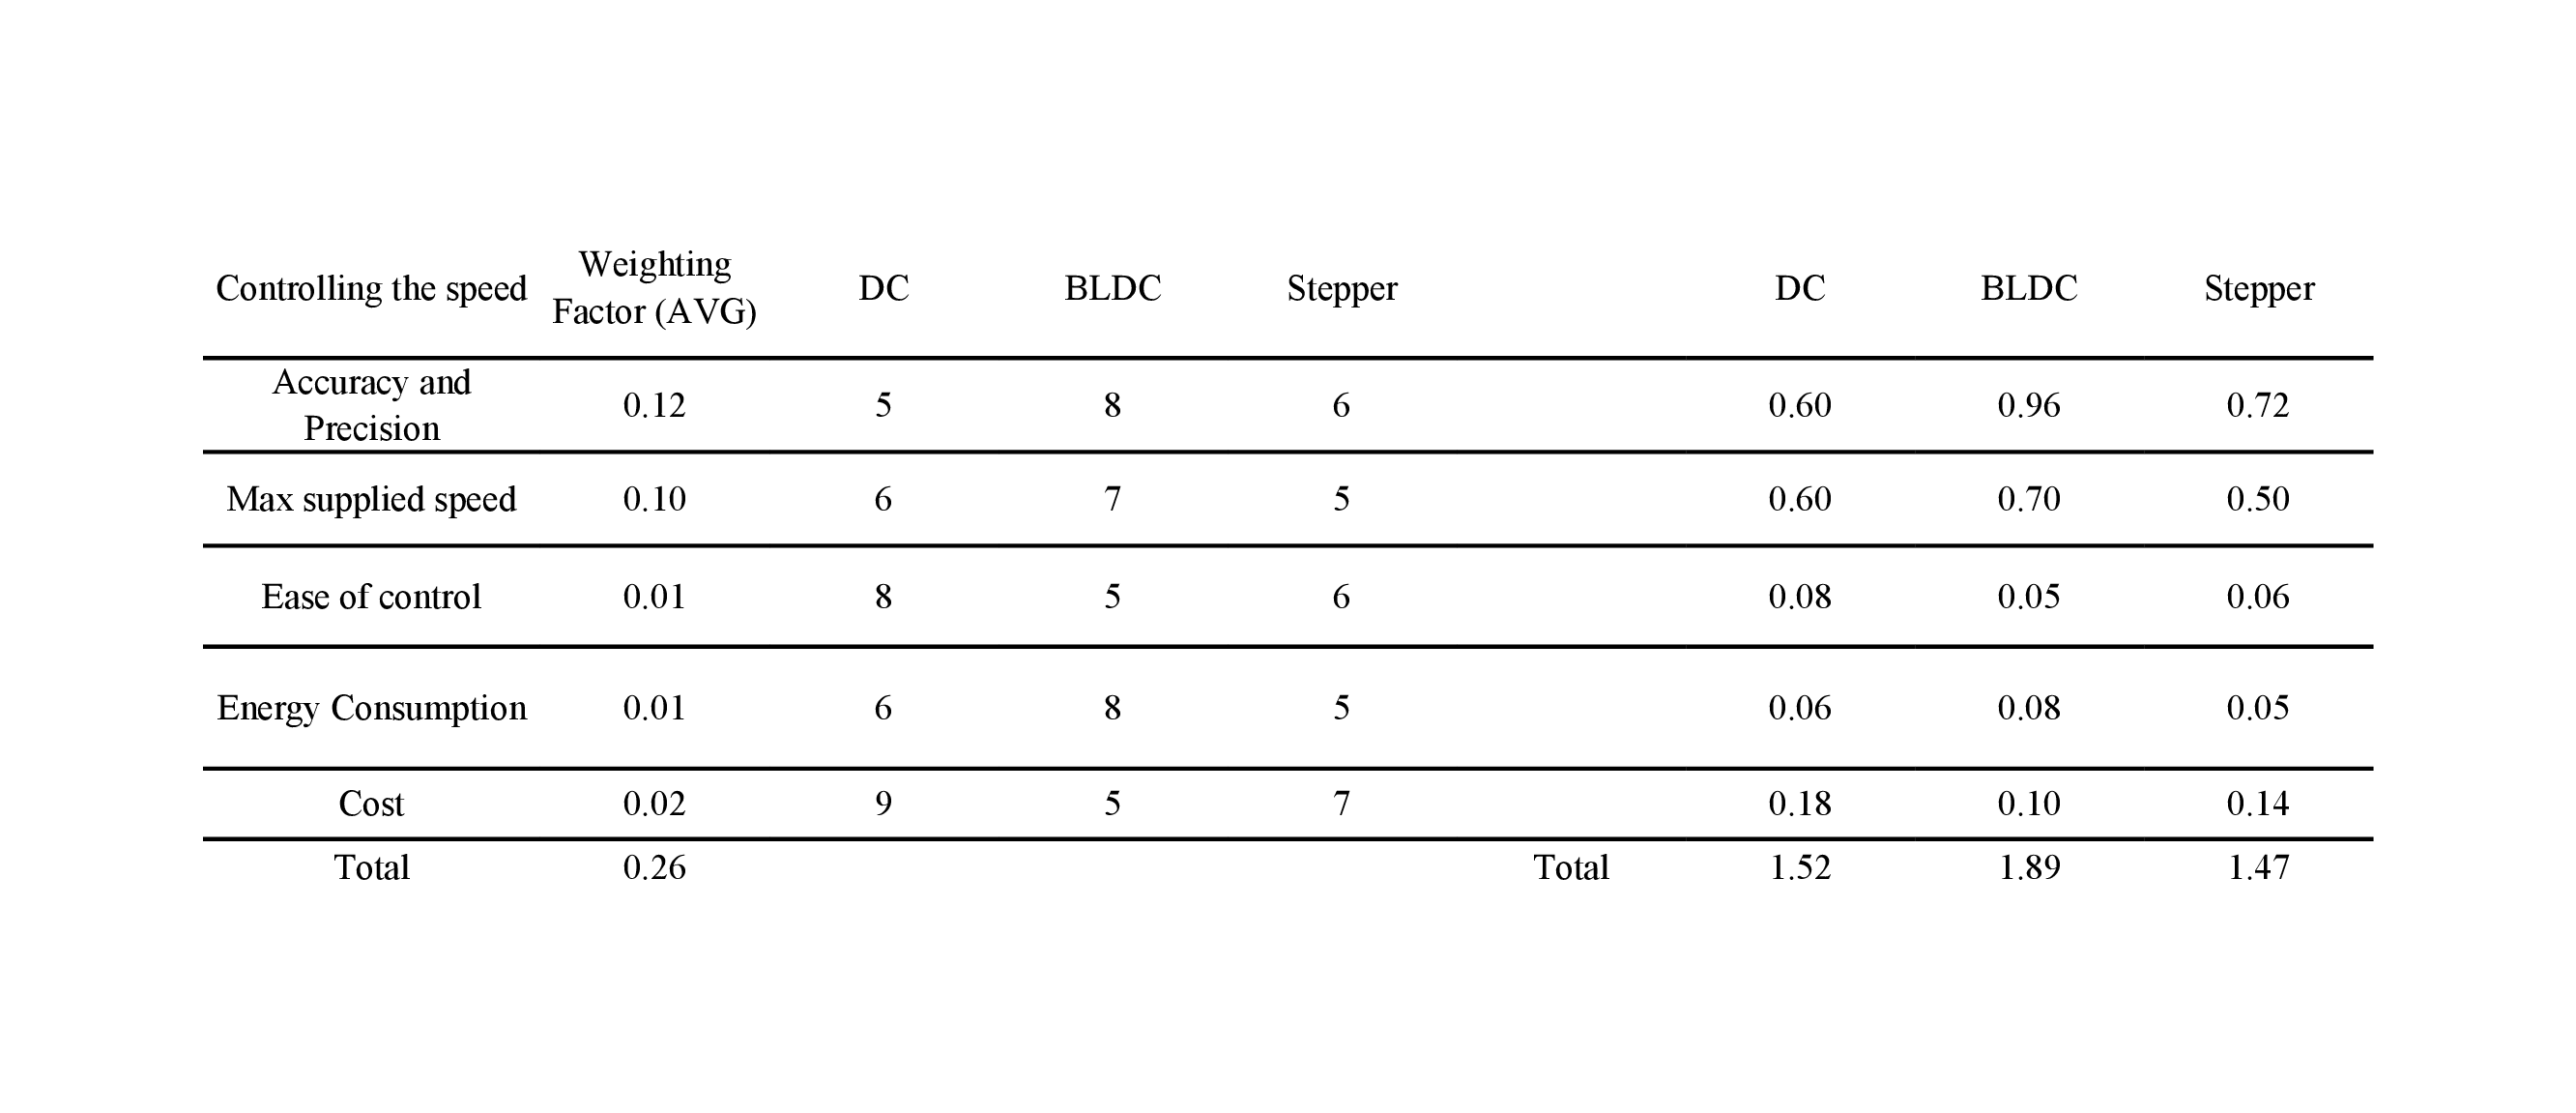
\includegraphics[width=1\textwidth]{Decision matrices/controlling speed.png}
    \caption{Controlling the speed}
\end{figure}

Six different solutions were proposed for providing the yaw angle to the mechanism, as outlined in the morphological chart. Among these, the solution referred to as "Gear 1" was identified as the optimal choice based on the decision matrix evaluation. This solution was selected due to its above-average performance across all criteria, making it the most balanced and effective option overall.

\begin{figure}[H]
    \centering
    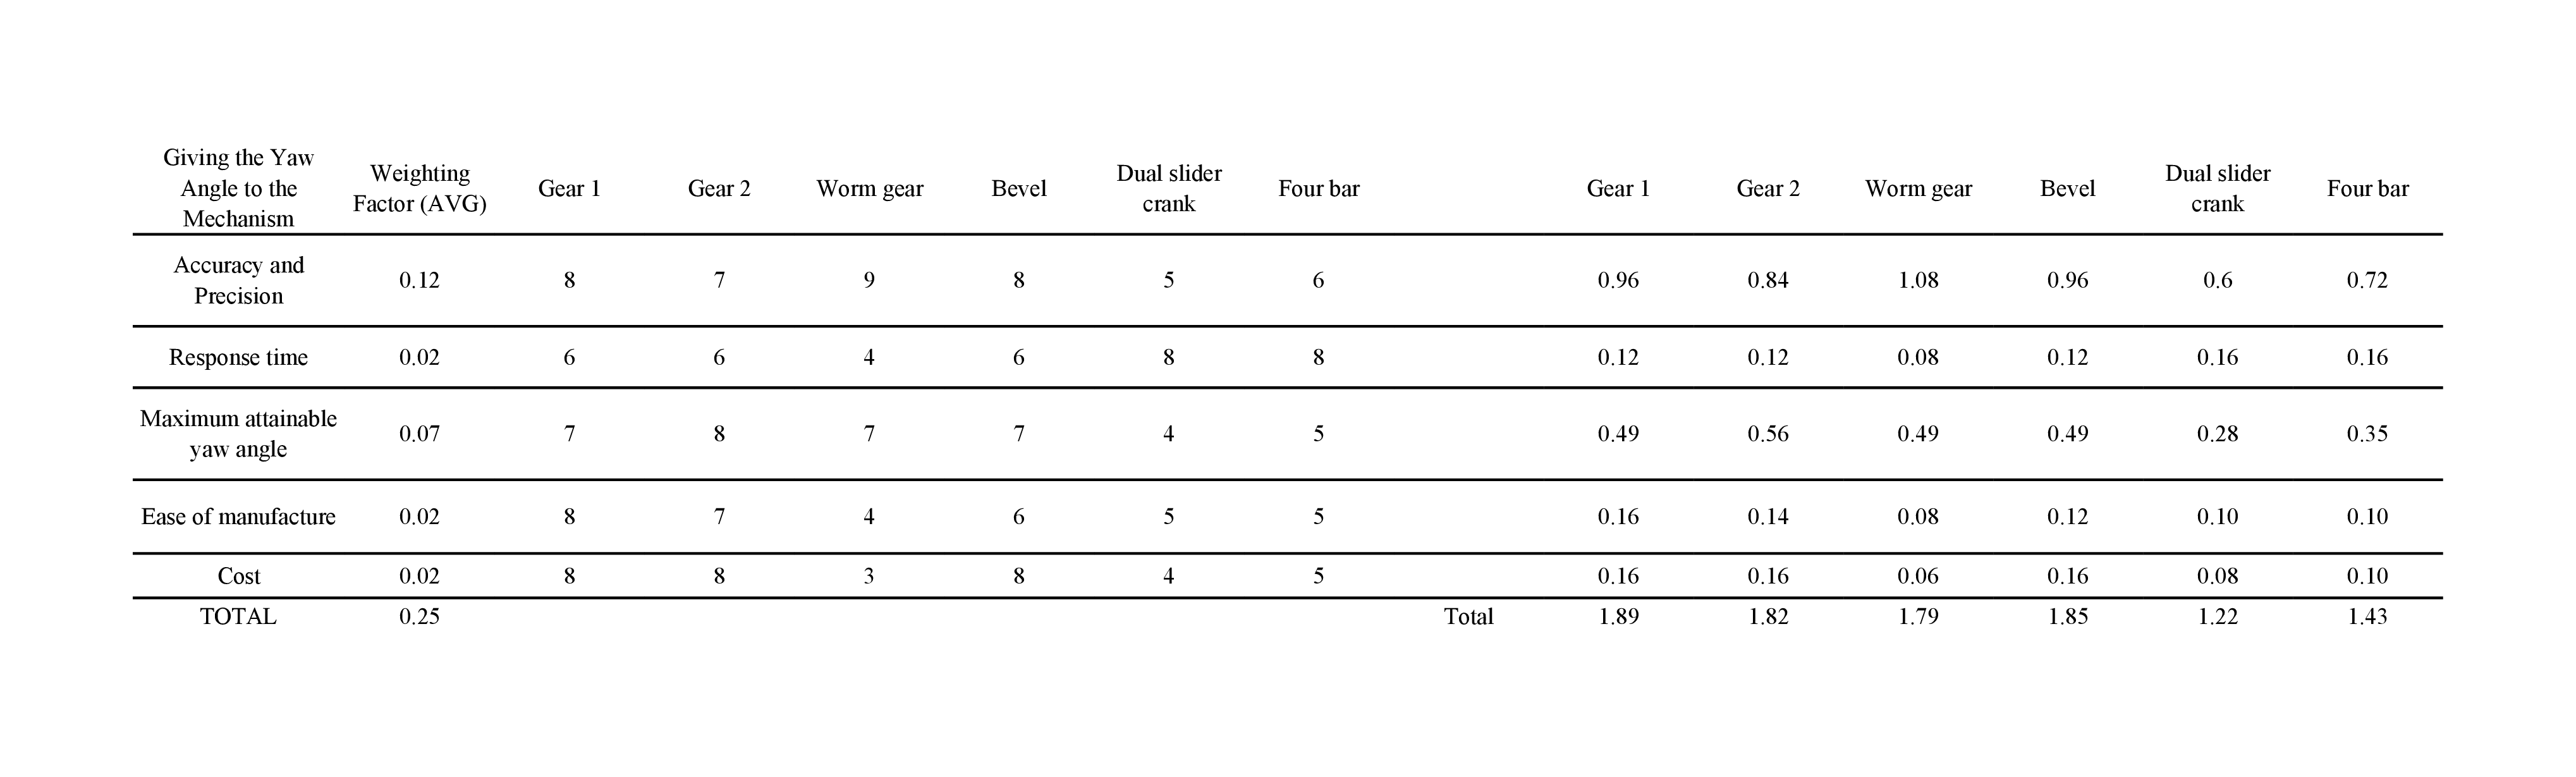
\includegraphics[width=1\textwidth]{Decision matrices/yaw.png}
    \caption{Giving yaw angle to the launching mechanism}
\end{figure}

For controlling the yaw angle, three motor alternatives were considered: servo, stepper, and DC with encoder. Based on the decision matrix evaluation, the servo motor was identified as the optimal solution. Its better accuracy and precision, along with its favorable cost, were key factors that made it the best choice for this application.

\begin{figure}[H]
    \centering
    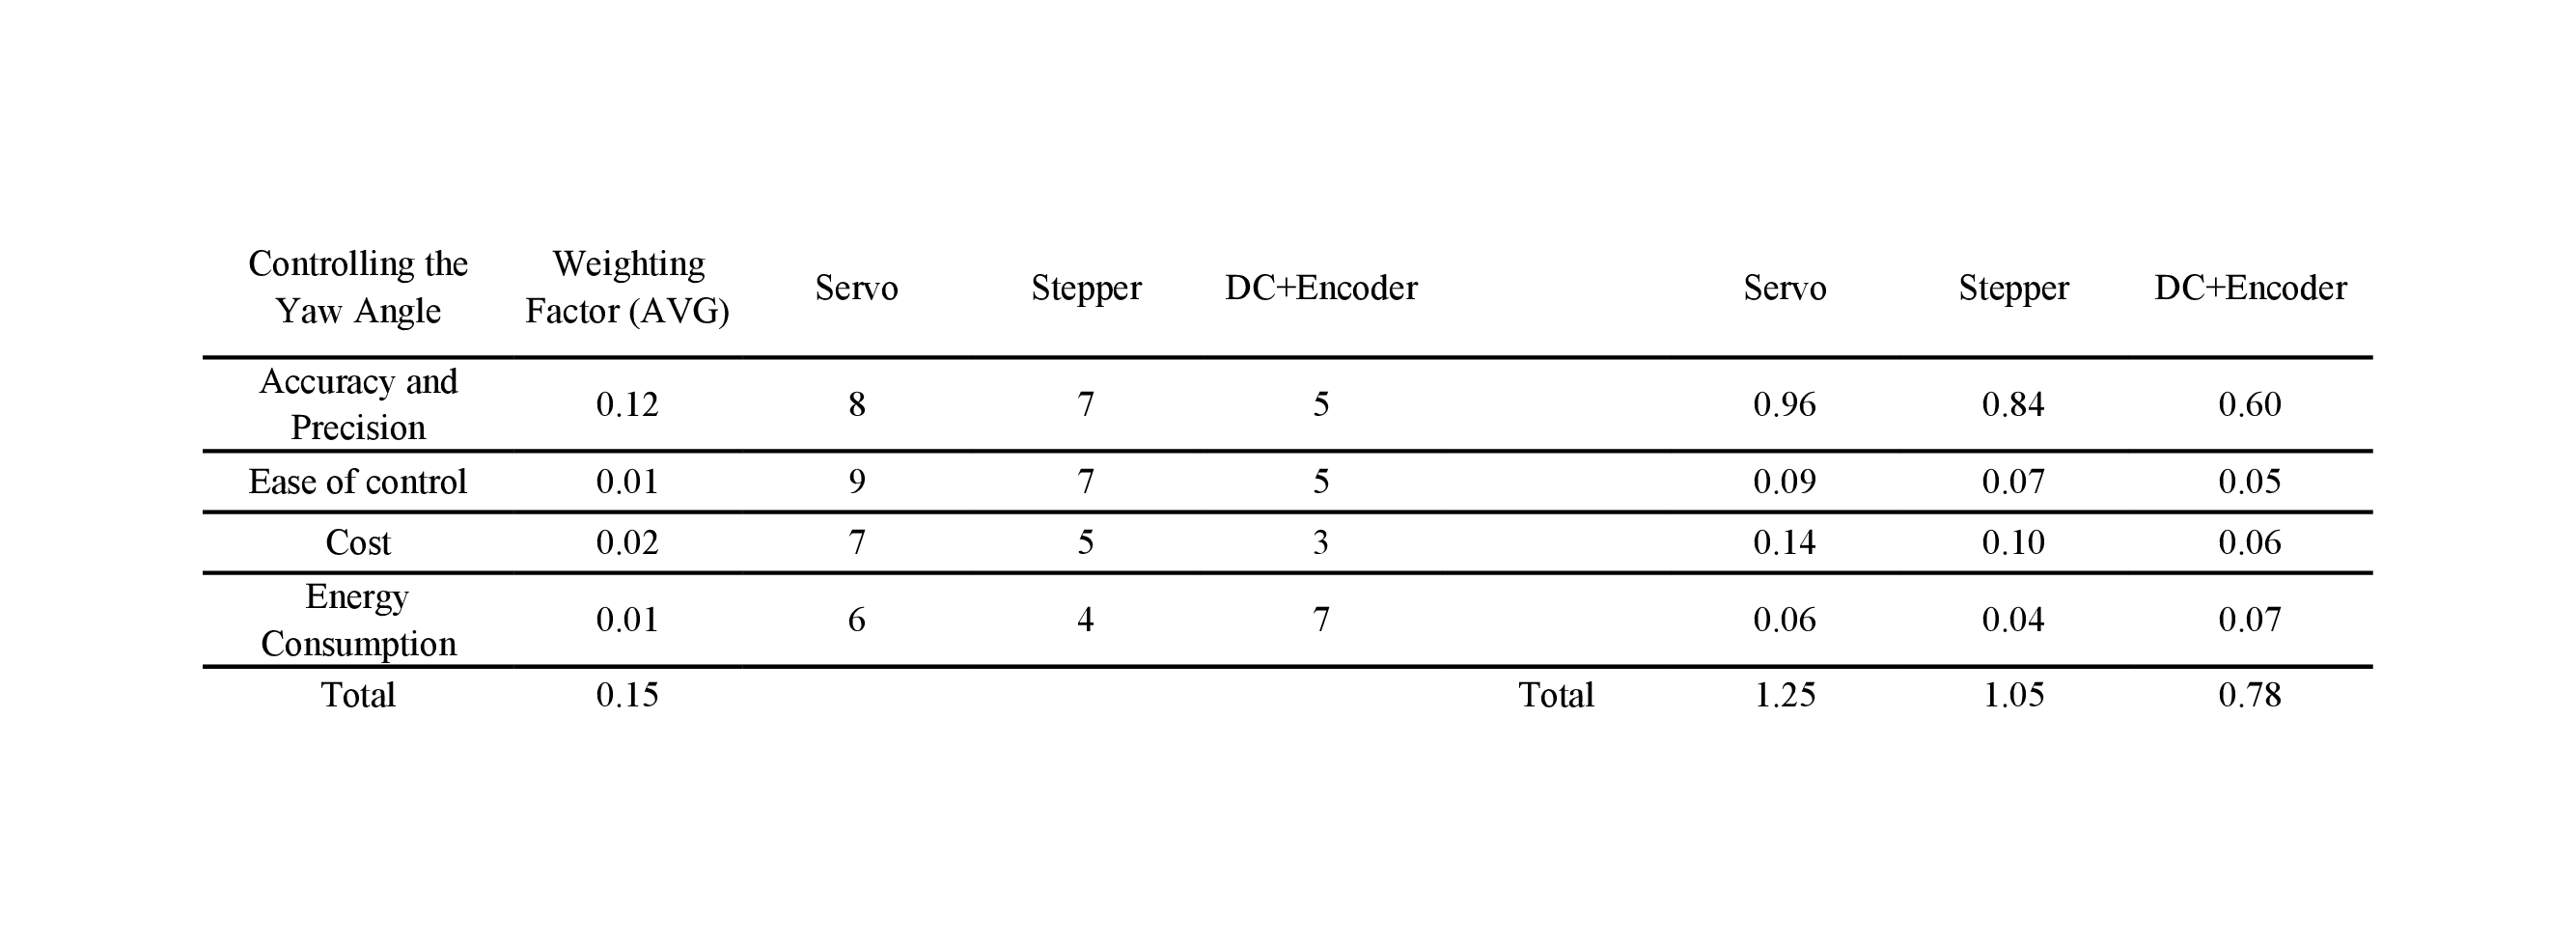
\includegraphics[width=1\textwidth]{Decision matrices/controlling yaw.png}
    \caption{Controlling the yaw angle}
\end{figure}

Six different solutions were proposed to give the pitch angle and, among them, the gear alternative was identified as the optimal solution. This choice was made based on its above-average performance across all criteria, making it the most suitable option to achieve the desired pitch angle.

\begin{figure}[H]
    \centering
    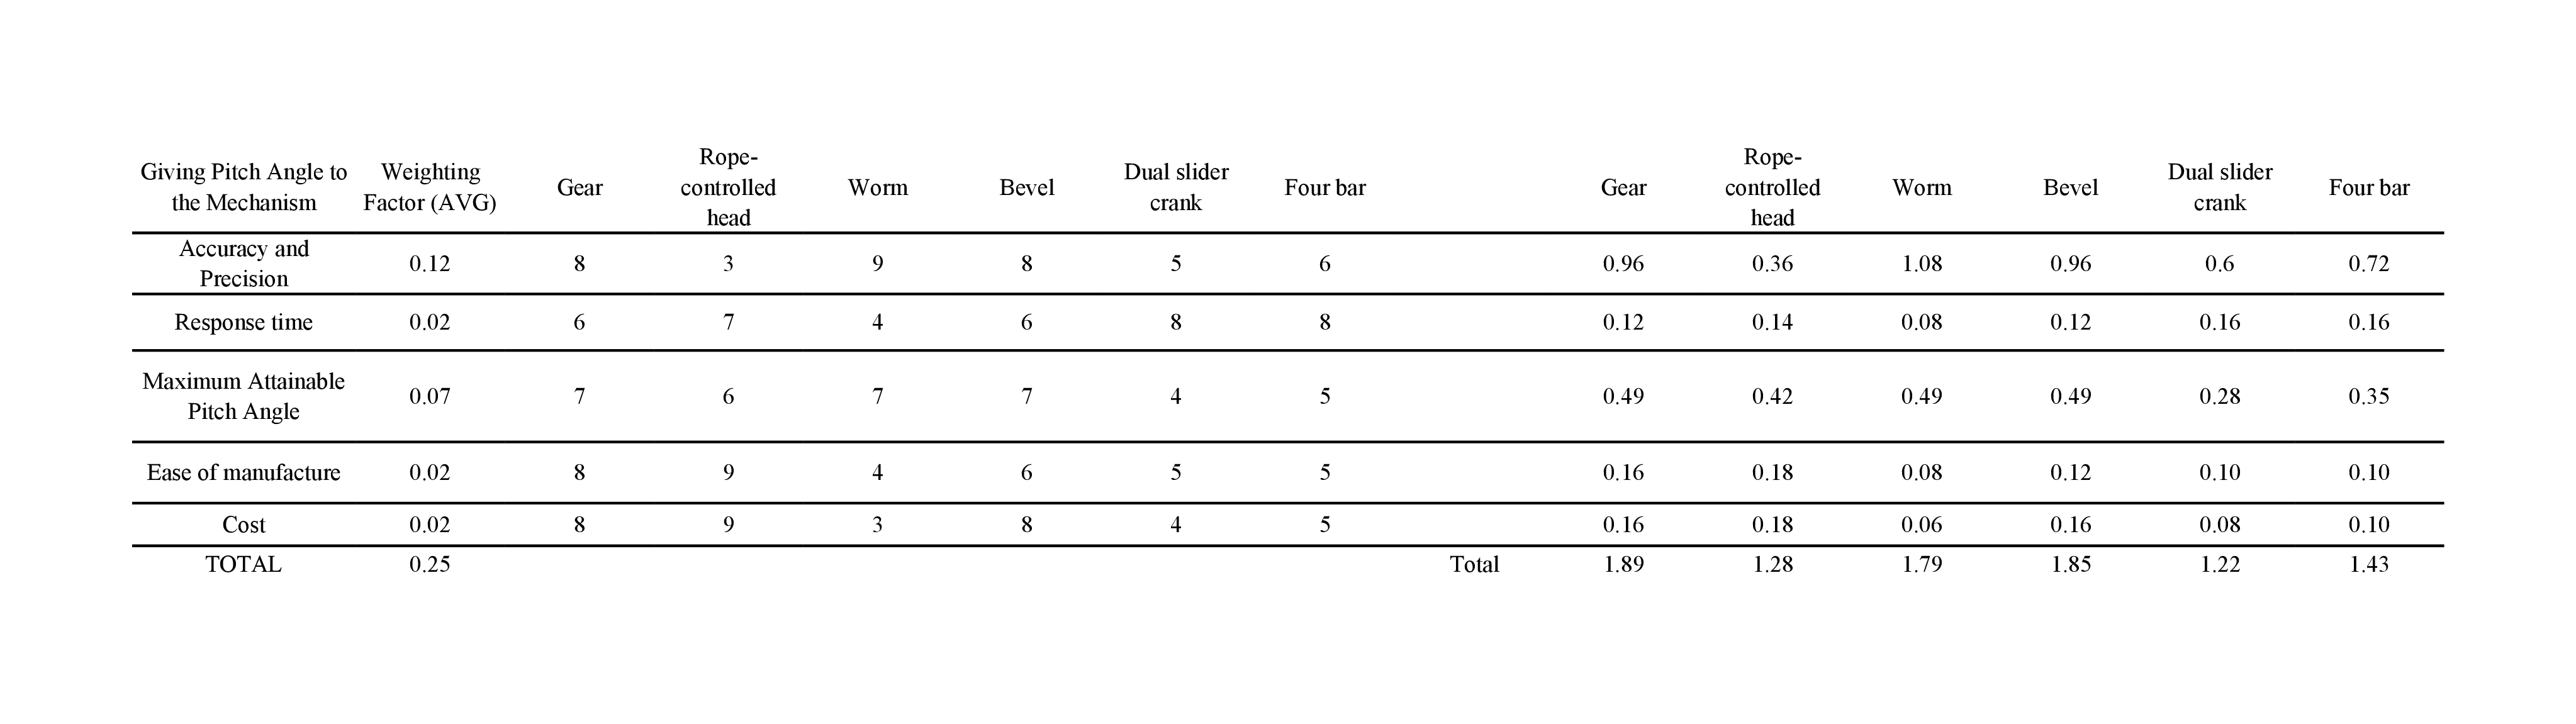
\includegraphics[width=1\textwidth]{Decision matrices/pitch.png}
    \caption{Giving pitch angle to the launching mechanism}
\end{figure}

For controlling the pitch angle, the same three alternatives as controlling the yaw angle were considered. Based on the evaluation of the decision matrix, the servomotor was identified as the optimal solution, similar to the selection to control the yaw angle.

\begin{figure}[H]
    \centering
    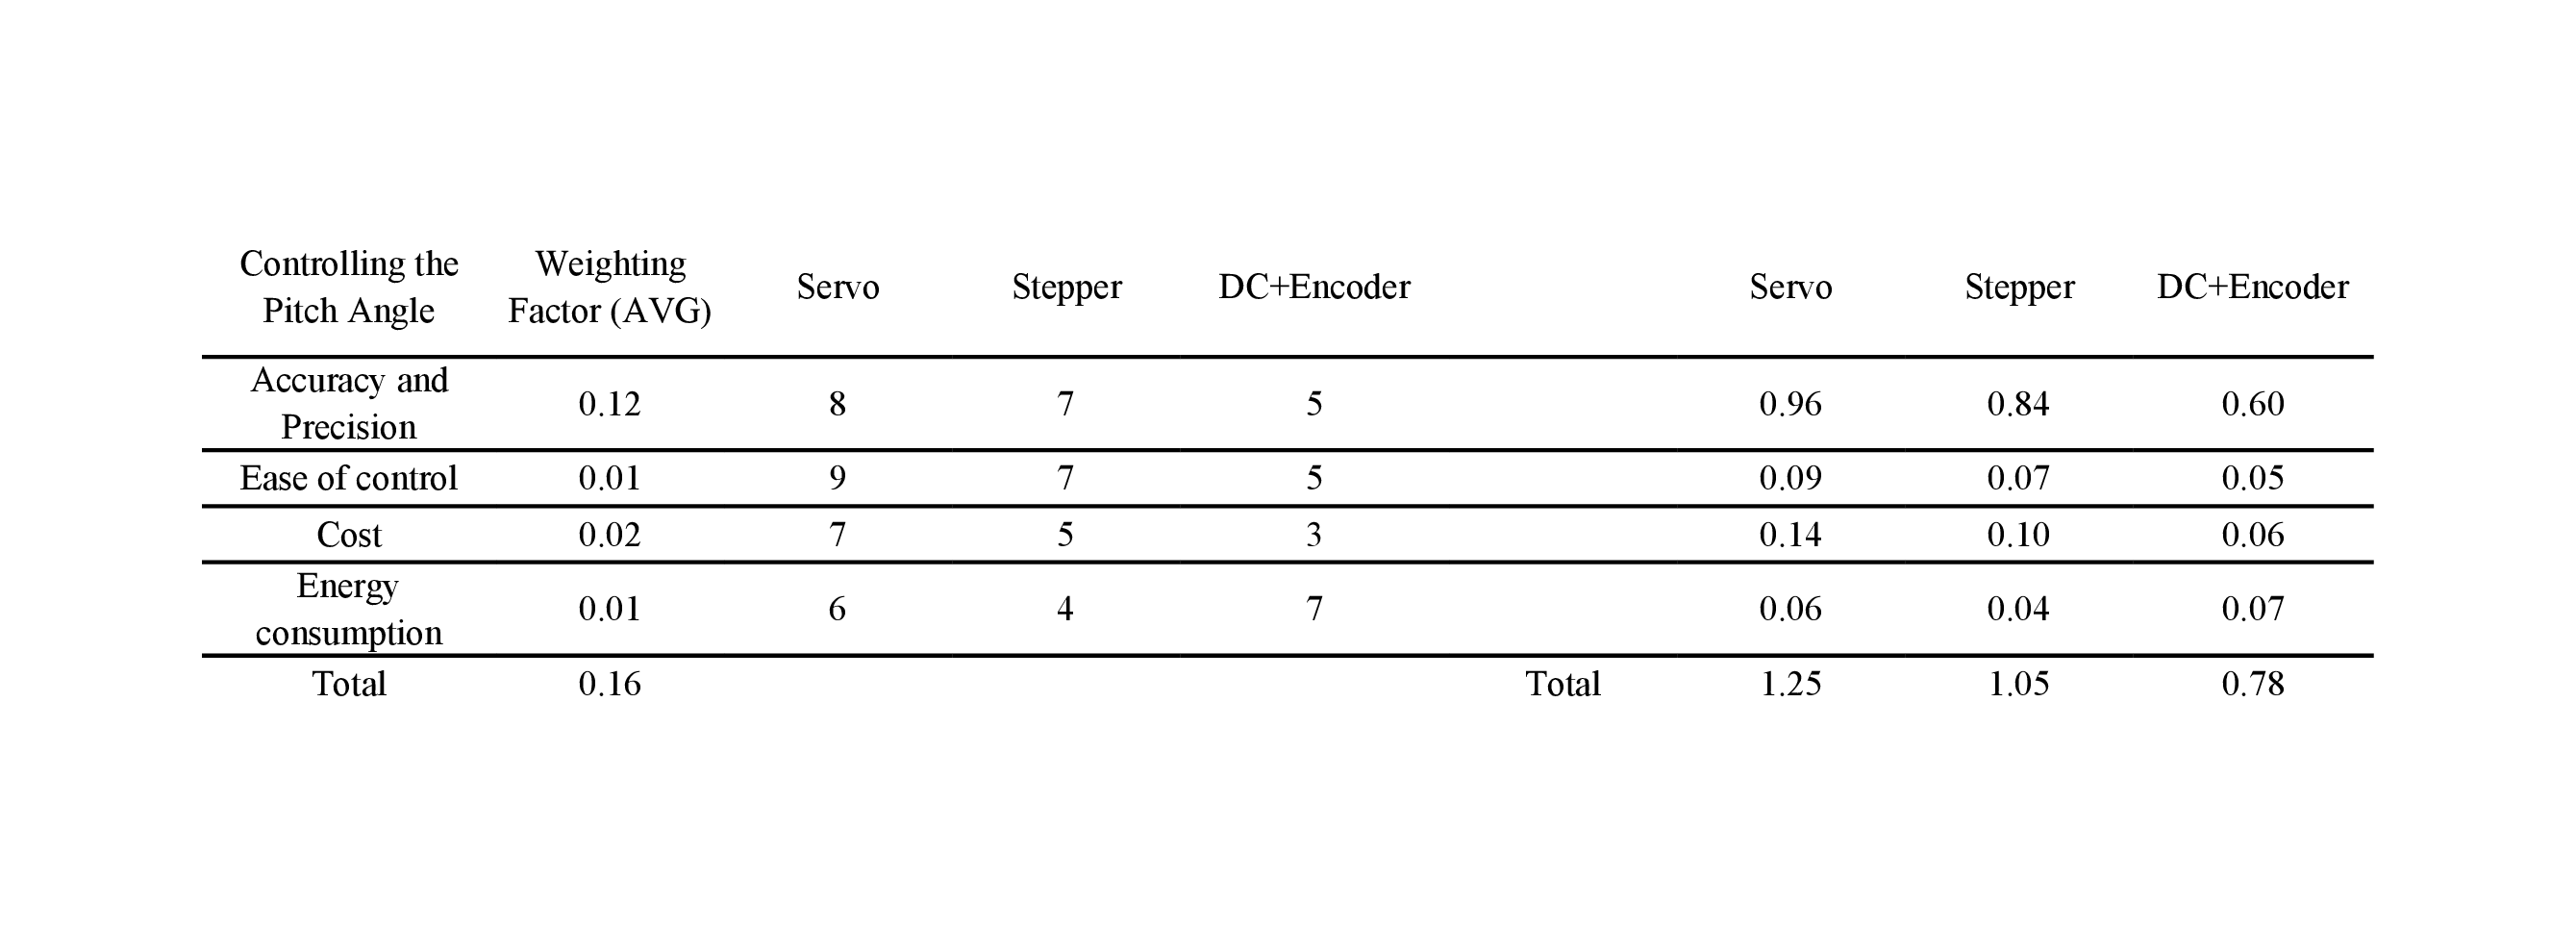
\includegraphics[width=1\textwidth]{Decision matrices/controlling pitch.png}
    \caption{Controlling the pitch angle}
\end{figure}

For accepting frequency information from the user, four alternatives were considered: integrated controller, IR remote, mobile, and wired remote. Based on the decision matrix evaluation, the integrated controller was identified as the optimal solution. Its advantages in terms of cost and ease of manufacture made it the best choice for this application.

\begin{figure}[H]
    \centering
    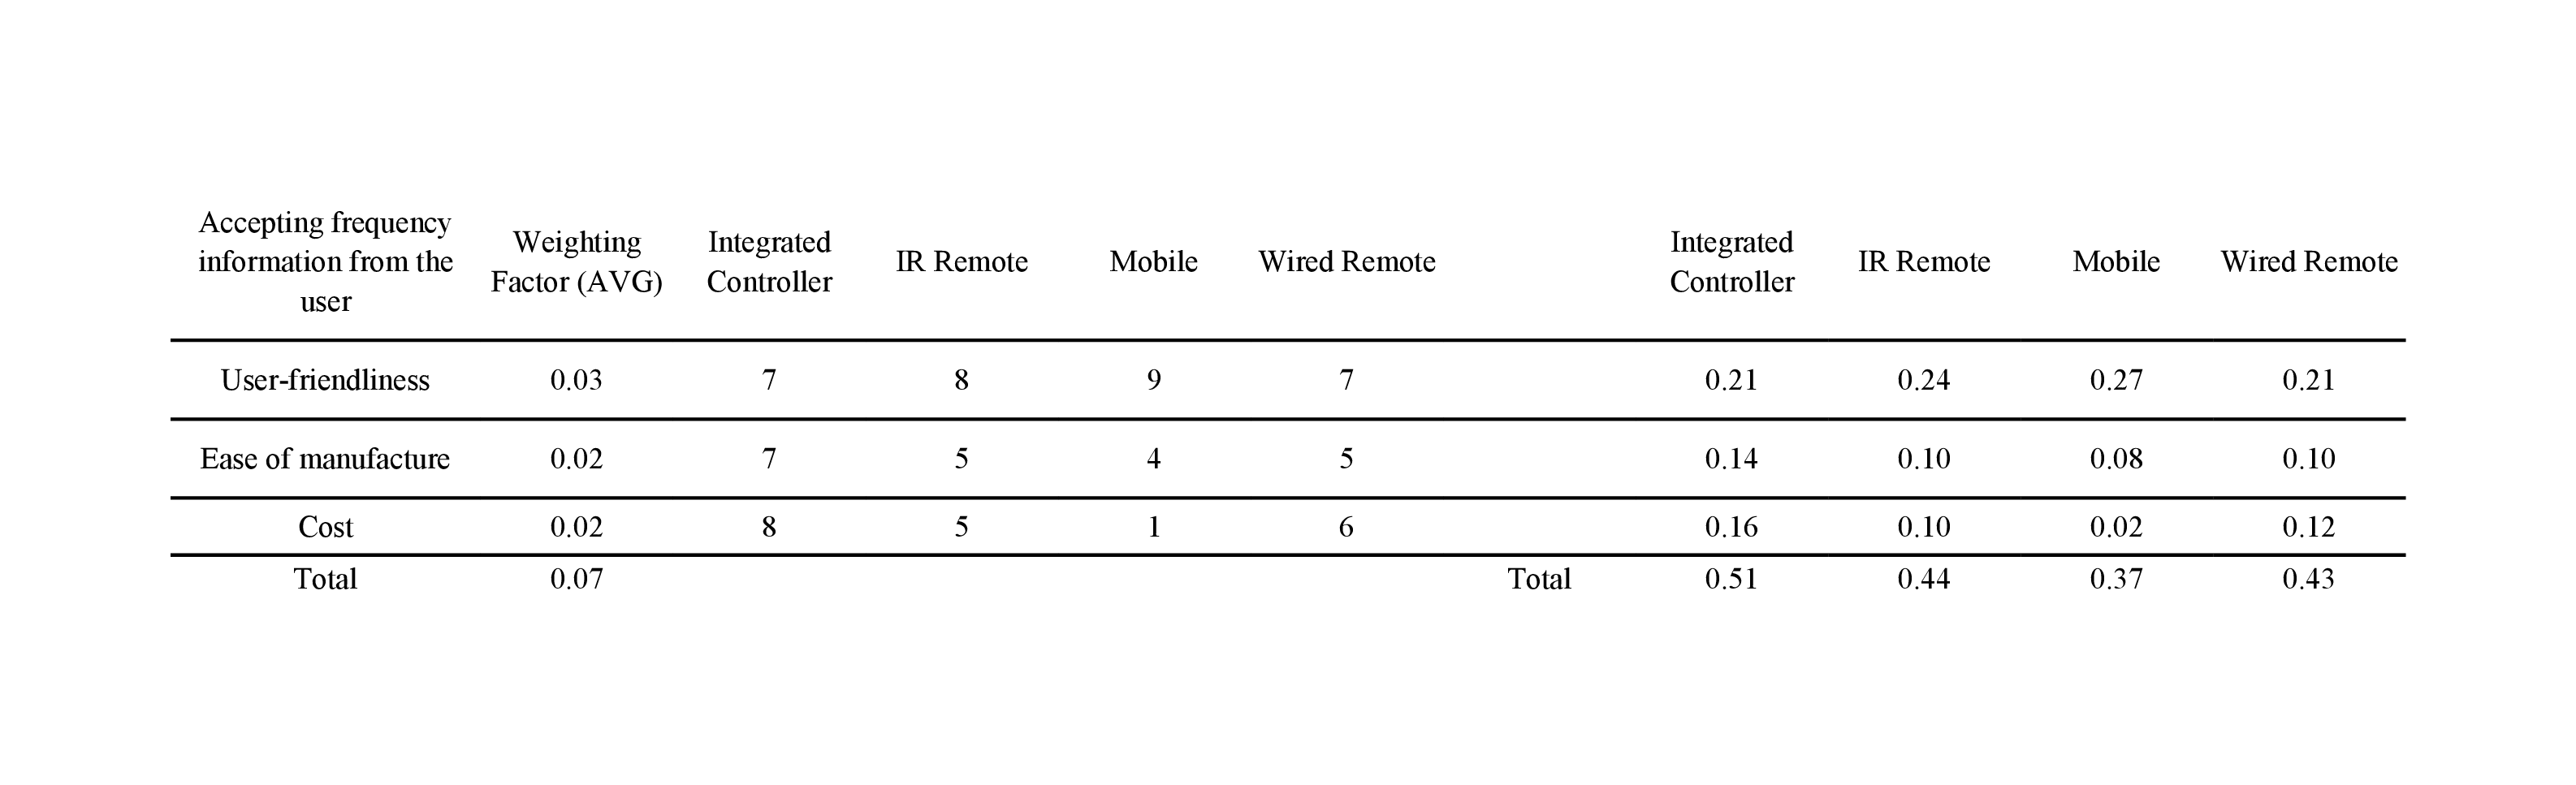
\includegraphics[width=1\textwidth]{Decision matrices/accept frequency.png}
    \caption{Accepting frequency information from the user}
\end{figure}

For accepting numerical information from the user, four alternatives were considered: potentiometer, encoder, touch screen, and button. Based on the decision matrix evaluation, the button was identified as the optimal solution. Its cost-effectiveness made it the best choice for this application.

\begin{figure}[H]
    \centering
    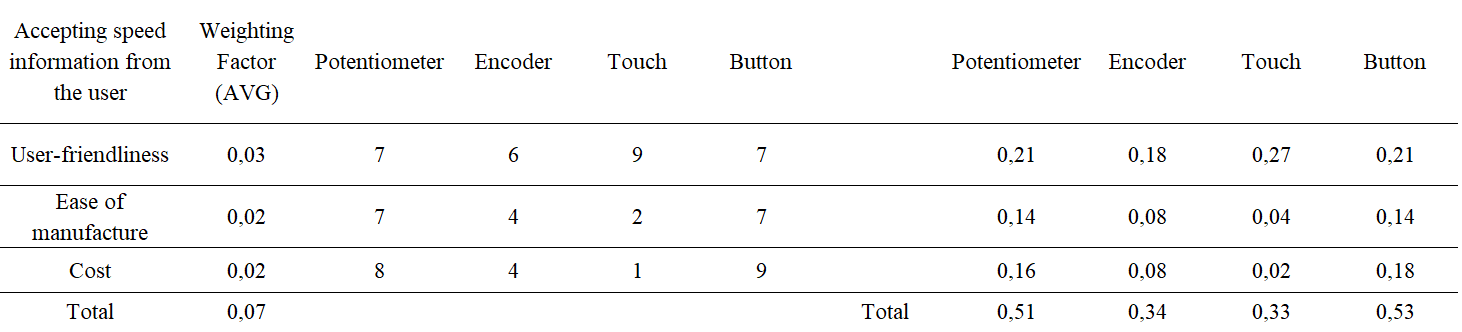
\includegraphics[width=1\textwidth]{Decision matrices/accept numerical.png}
    \caption{Accepting numerical information from the user}
\end{figure}

For accepting trajectory information from the user, the same four alternatives were considered. Similarly, the evaluation of the decision matrix identified the integrated controller as the optimal solution.

\begin{figure}[H]
    \centering
    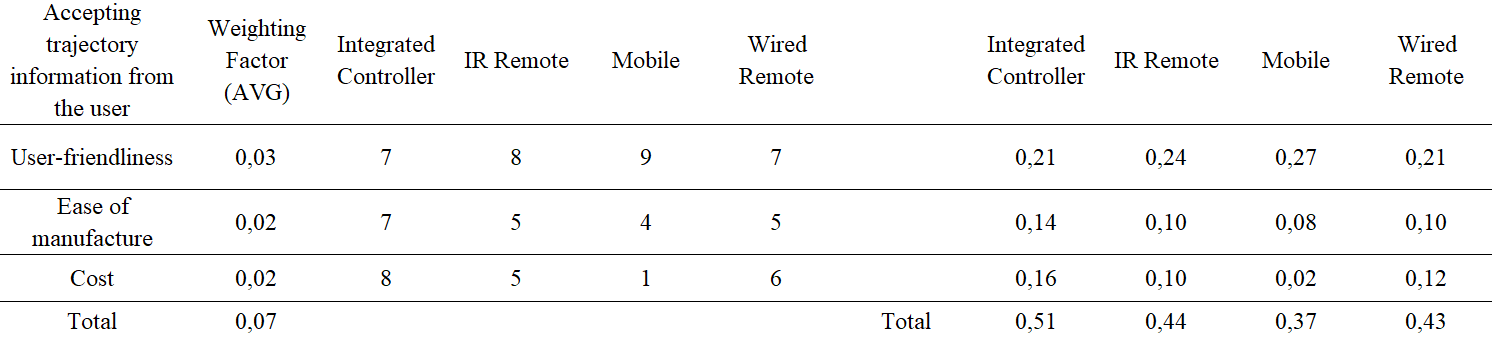
\includegraphics[width=1\textwidth]{Decision matrices/accept traj.png}
    \caption{Accepting trajectory information from the user}
\end{figure}


For allowing the user to position the device, five alternatives were considered: clamp, magnet, suction, rail, and wheel. Based on the decision matrix evaluation, the clamp was identified as the optimal solution. It demonstrated above-average performance across all criteria, making it the best choice for this application.

\begin{figure}[H]
    \centering
    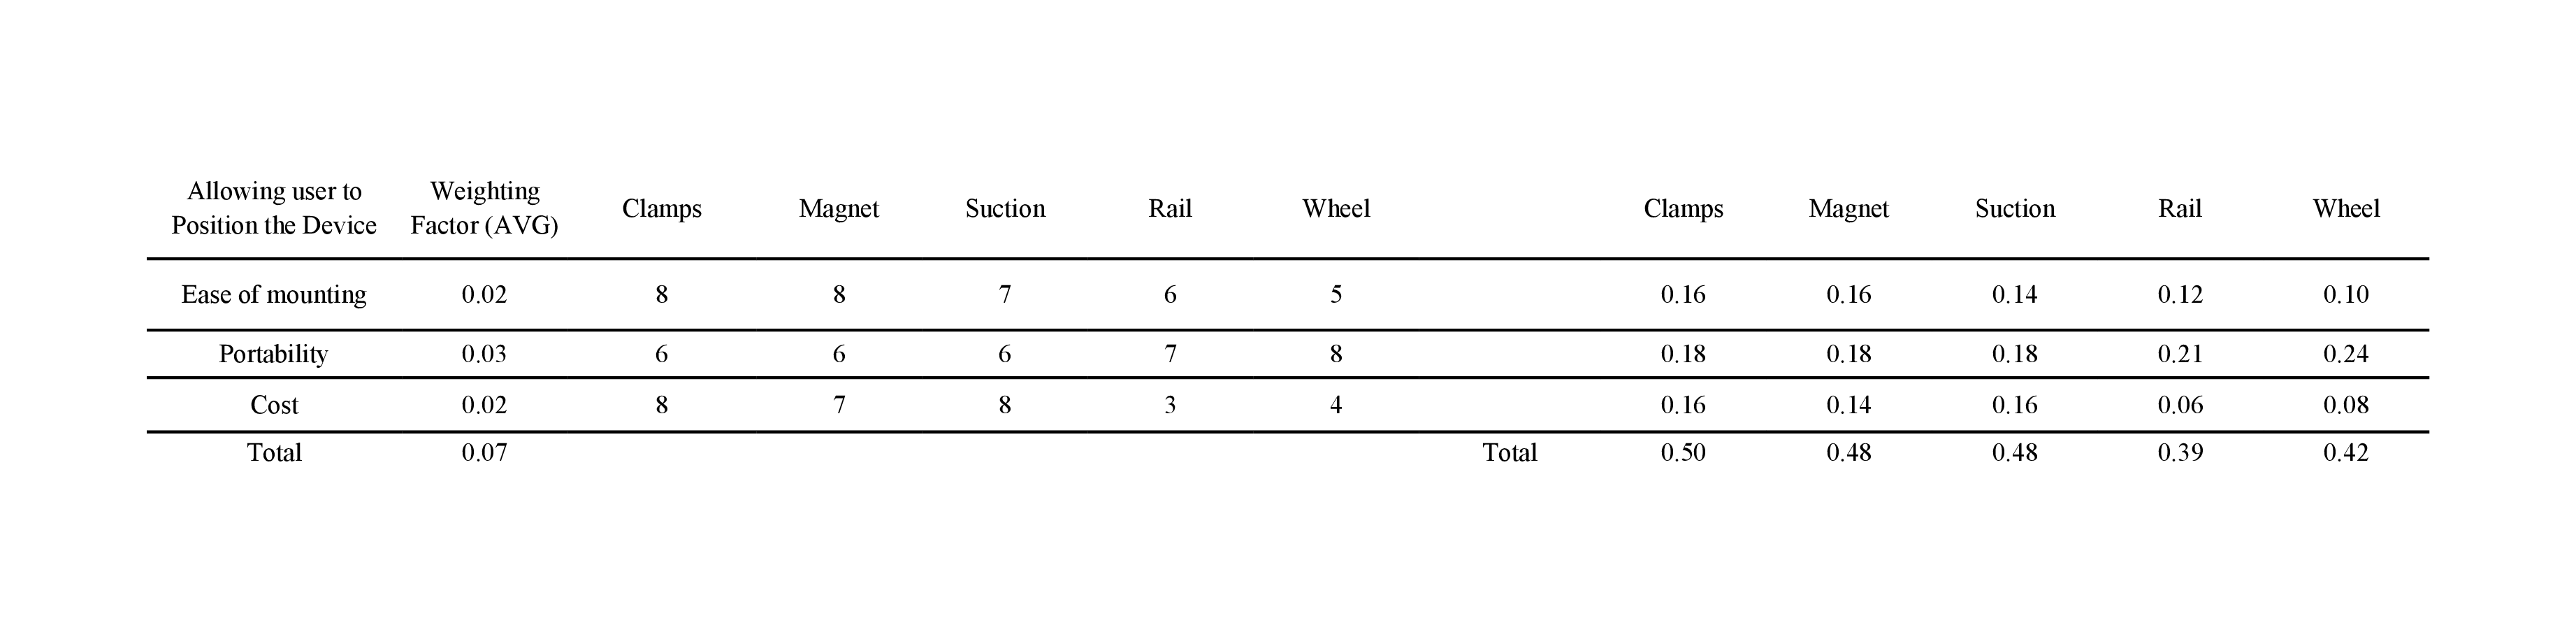
\includegraphics[width=1\textwidth]{Decision matrices/position device.png}
    \caption{Allowing the user to position the device}
\end{figure}

For preventing balls from escaping, three alternatives were considered: net, spherical wall, and wipers with net. Based on the decision matrix evaluation, the net was identified as the optimal solution. Its advantages in terms of portability, cost, and ease of manufacture made it the best choice for this application.

\begin{figure}[H]
    \centering
    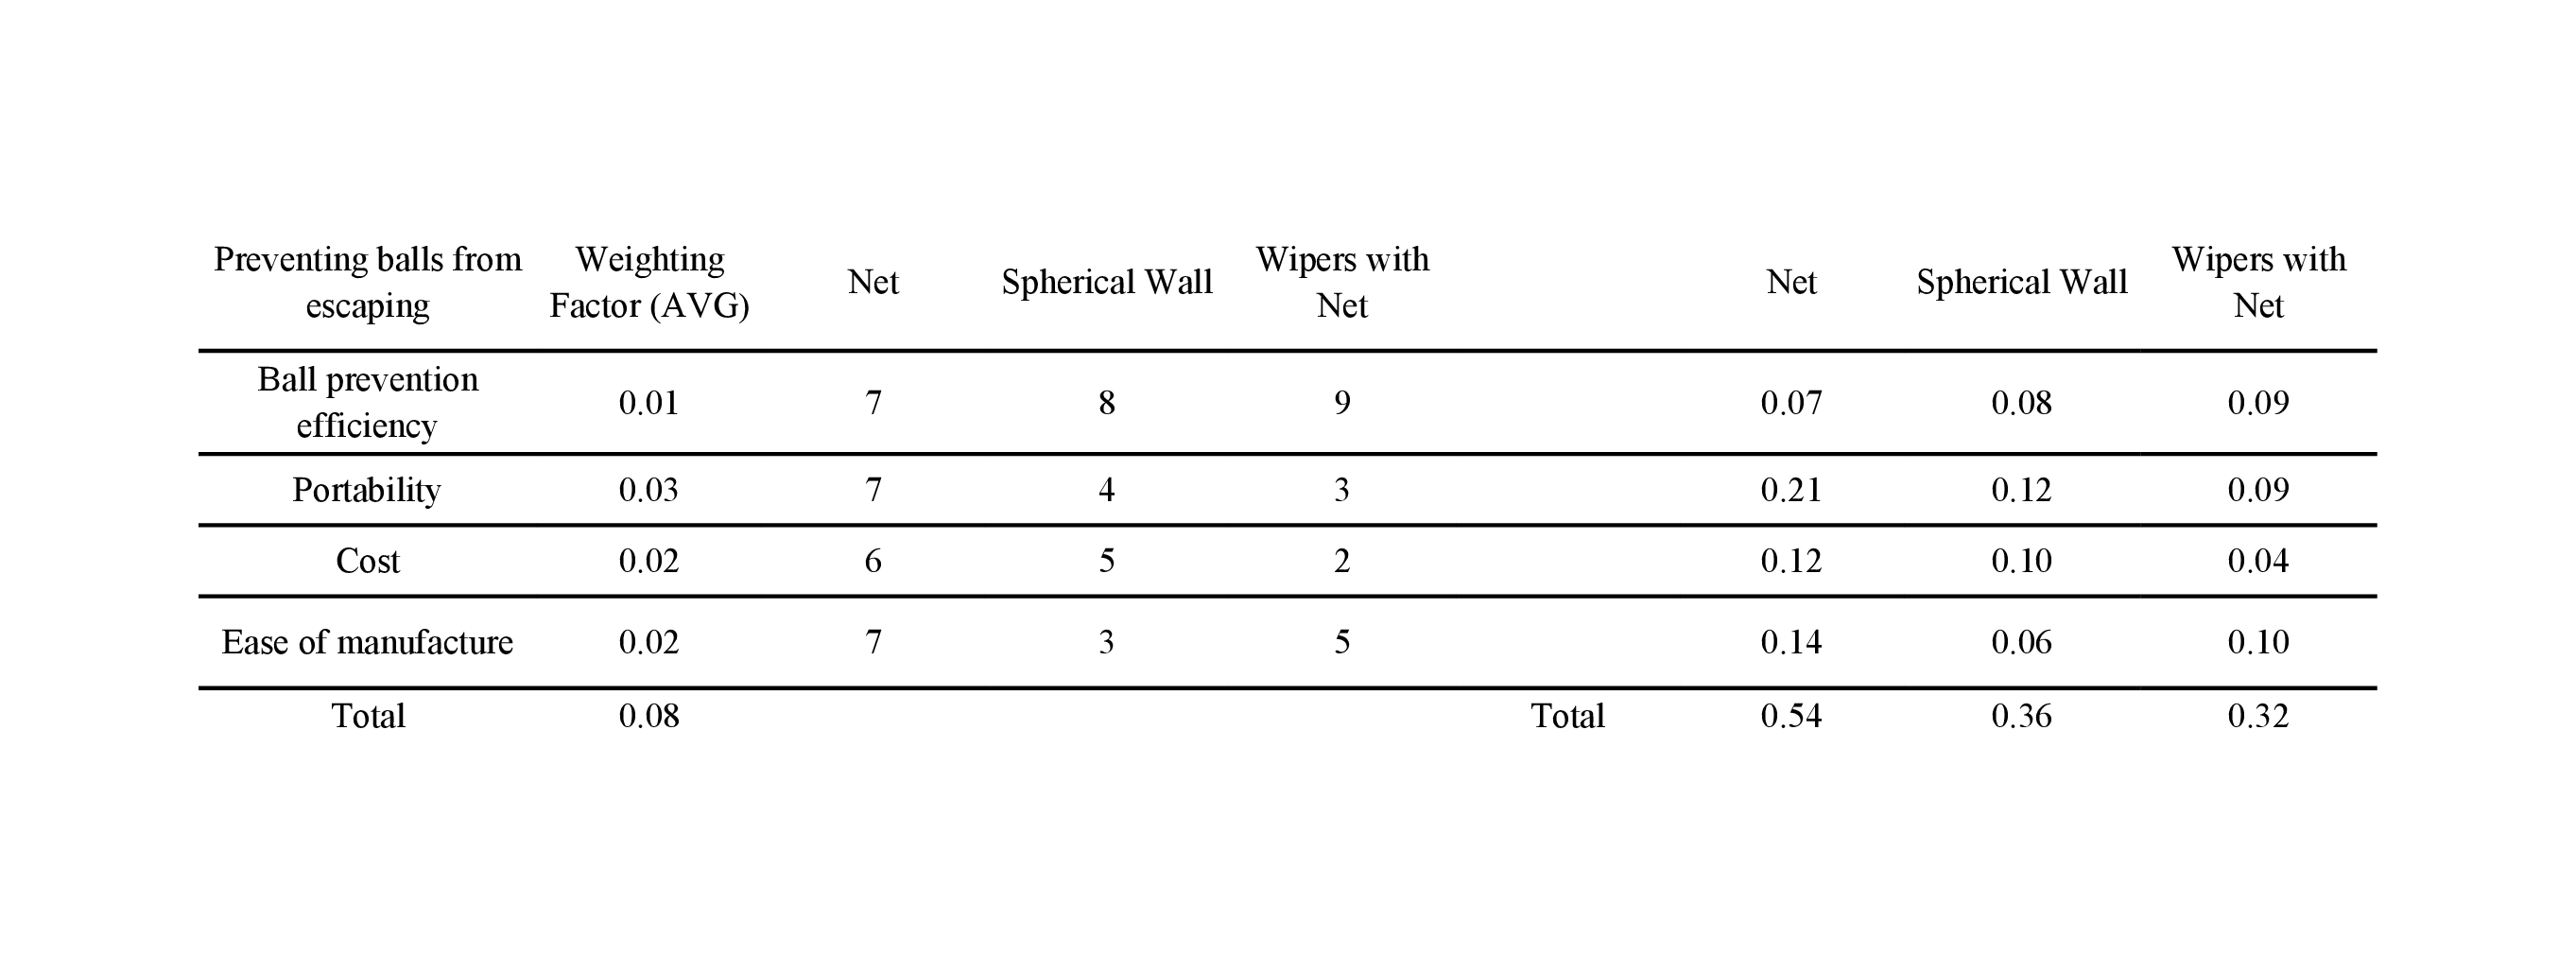
\includegraphics[width=1\textwidth]{Decision matrices/prevent escaping.png}
    \caption{Preventing balls from escaping}
\end{figure}

For storing the balls, four alternatives were considered: box, tunnel, groove, and gravity funnel. Based on the decision matrix evaluation, the groove was identified as the optimal solution. Its advantages in terms of capacity and portability made it the best choice for this application.

\begin{figure}[H]
    \centering
    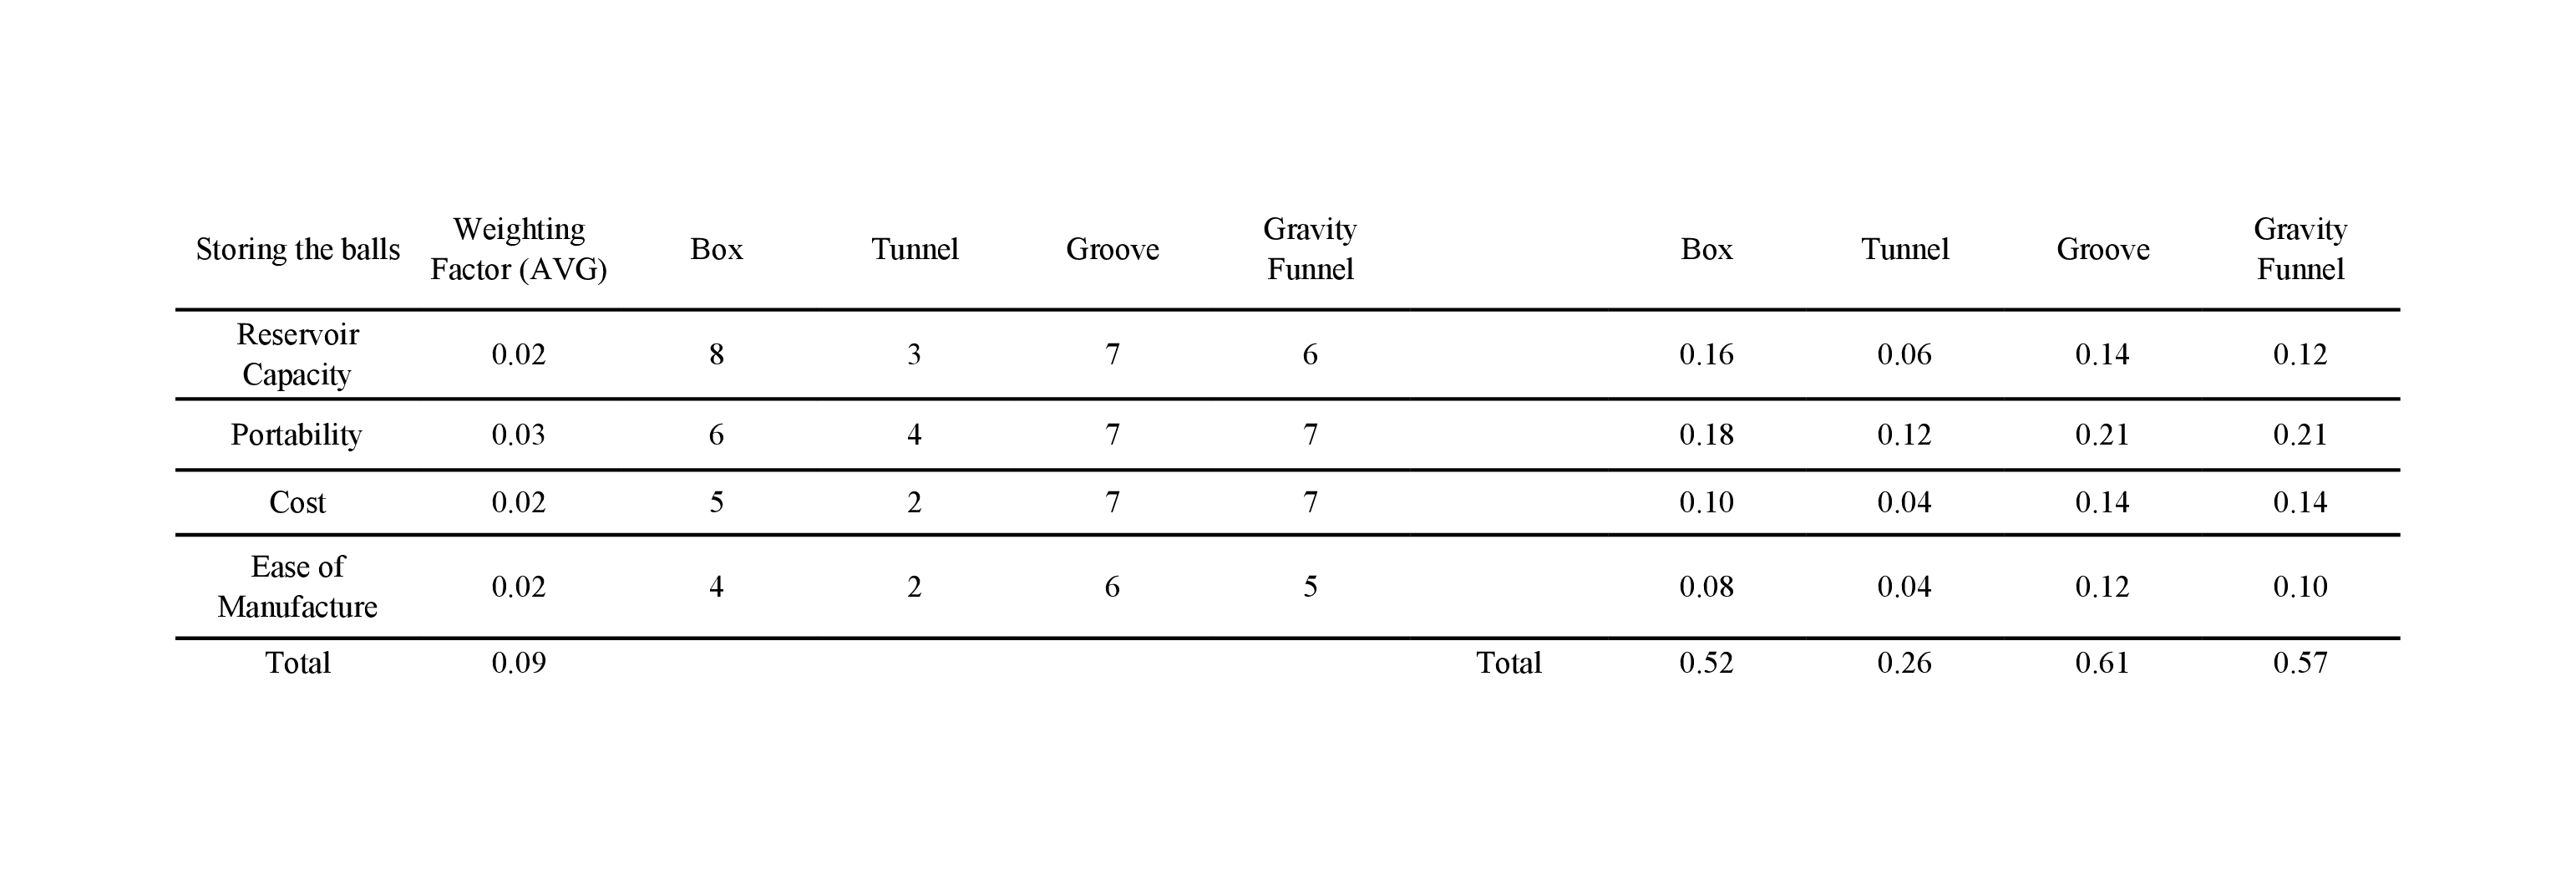
\includegraphics[width=1\textwidth]{Decision matrices/storing.png}
    \caption{Storing the balls}
\end{figure}
For transferring balls from storage, four alternatives were considered: Maltese wheel, spiral lift, translating box, and belt mechanism. Based on the decision matrix evaluation, the Maltese wheel was identified as the optimal solution. It demonstrated the best overall performance across all criteria, making it the most suitable choice for this application.

\begin{figure}[H]
    \centering
    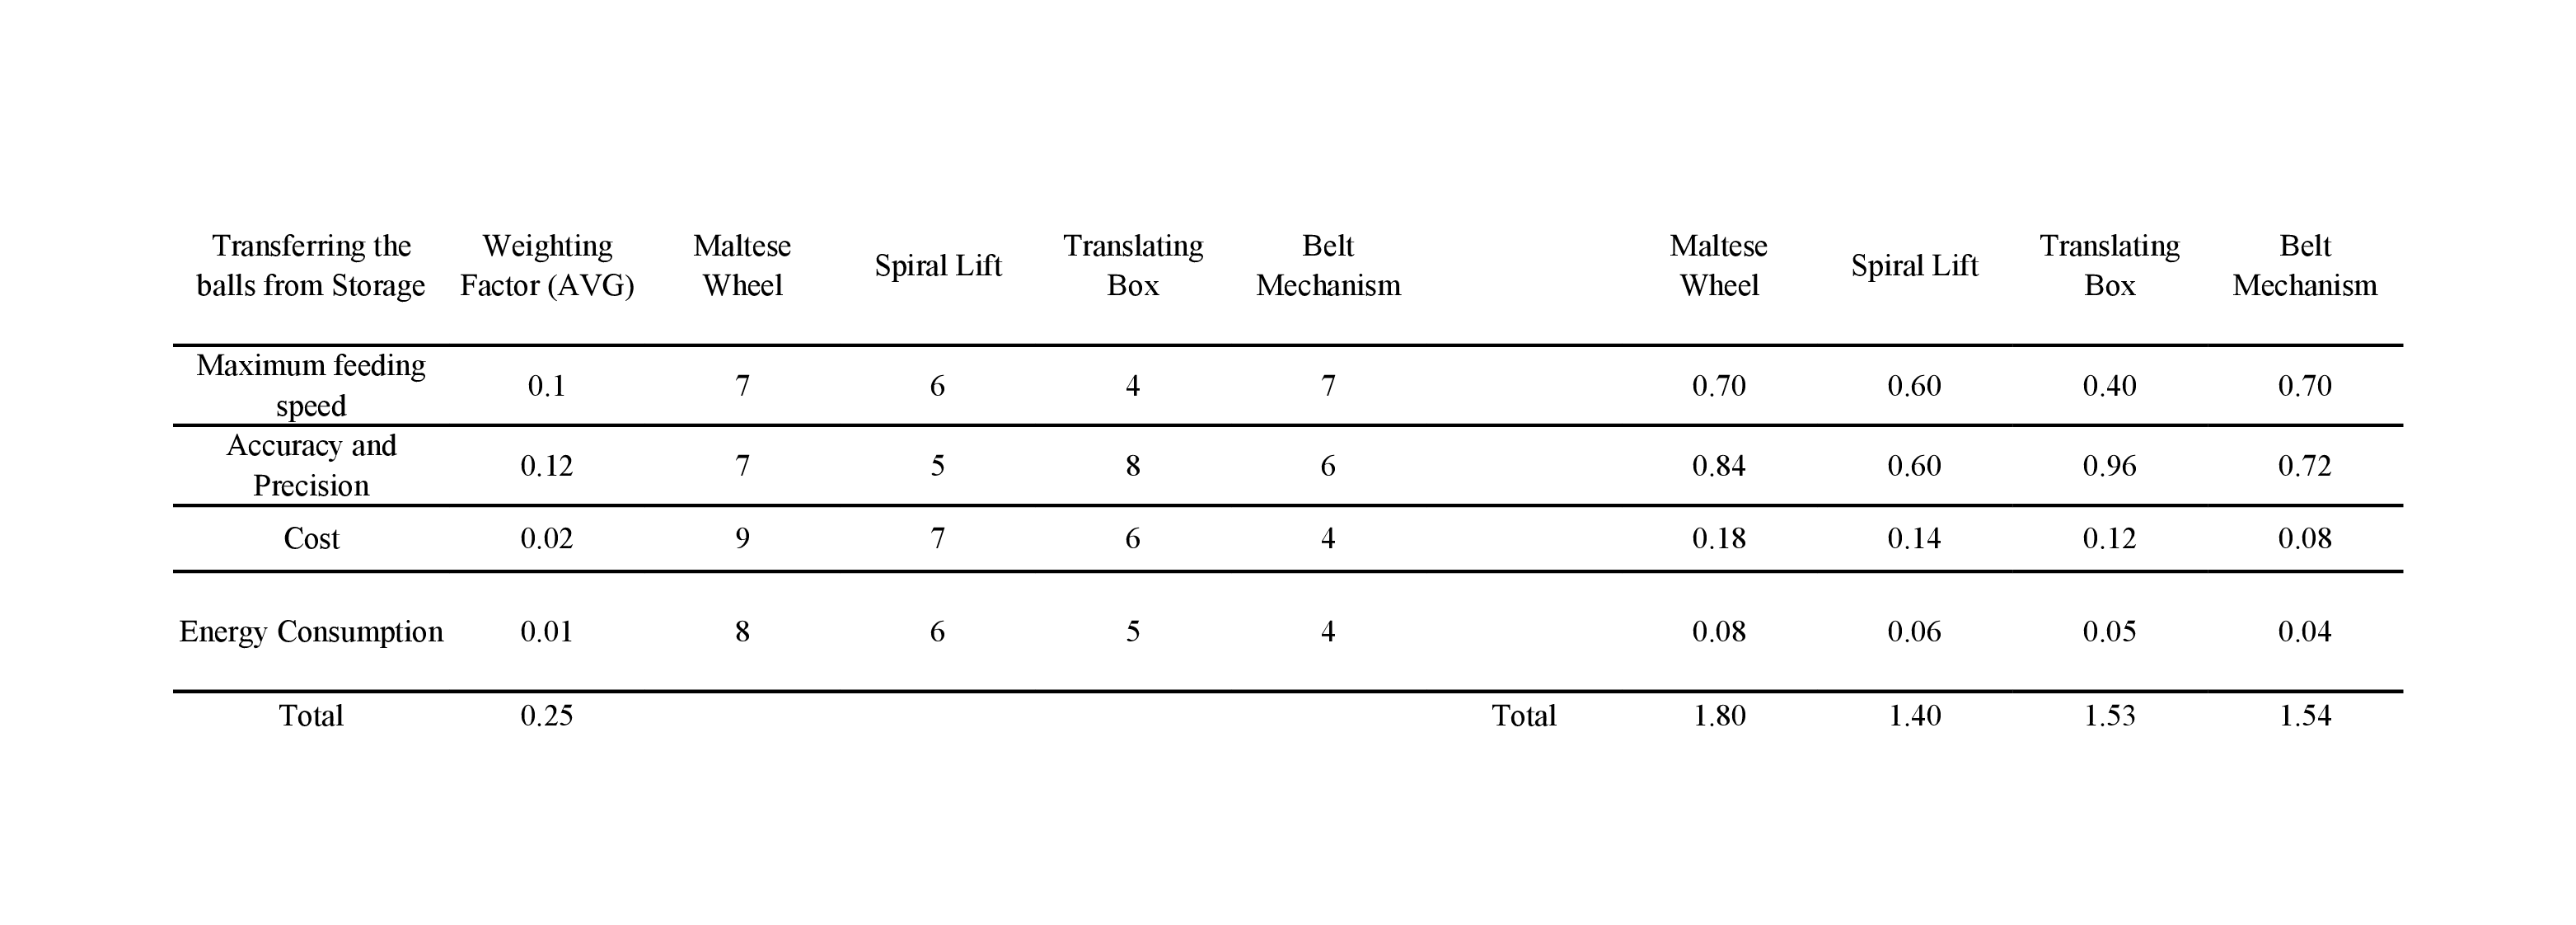
\includegraphics[width=1\textwidth]{Decision matrices/transfer from storage.png}
    \caption{Transferring the balls from  the storage} 
\end{figure}

For controlling the ball feed for storage, three alternatives were considered: stepper, DC, and DC with encoder. Based on the decision matrix evaluation, the stepper motor was identified as the optimal solution. It demonstrated above-average performance across all criteria, making it the most suitable choice for this application.

\begin{figure}[H]
    \centering
    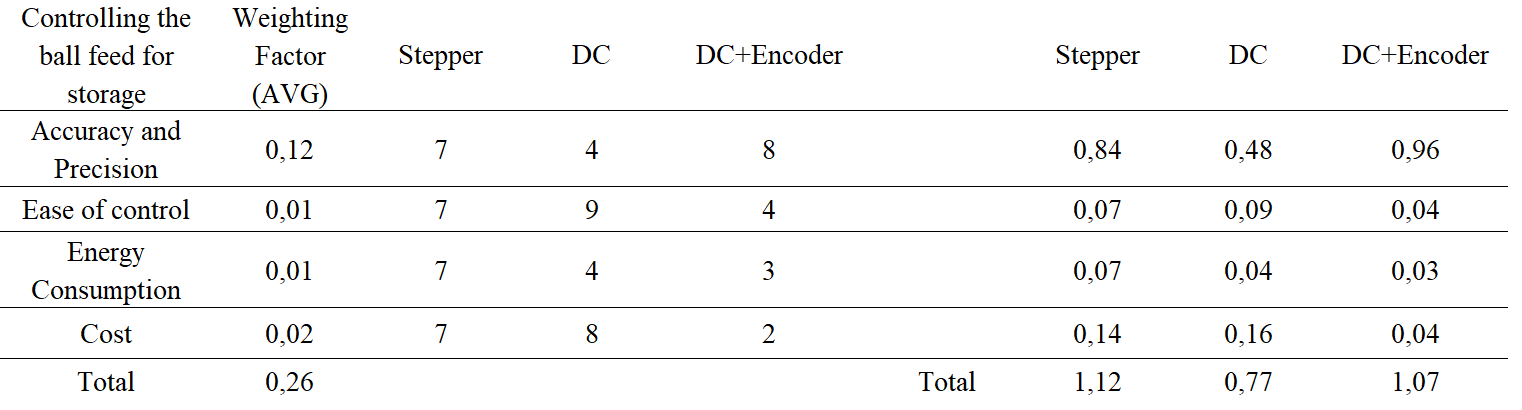
\includegraphics[width=1\textwidth]{Decision matrices/controlling ball feed for storage.png}
    \caption{Controlling the ball feed for storage}
\end{figure}

For transferring balls to launch, four alternatives were considered: Maltese wheel, spiral lift, rotating pusher, and belt mechanism. Based on the evaluation of the decision matrix, the Maltese wheel was identified as the optimal solution. It demonstrated above-average performance across all criteria, making it the most suitable choice for this application.

\begin{figure}[H]
    \centering
    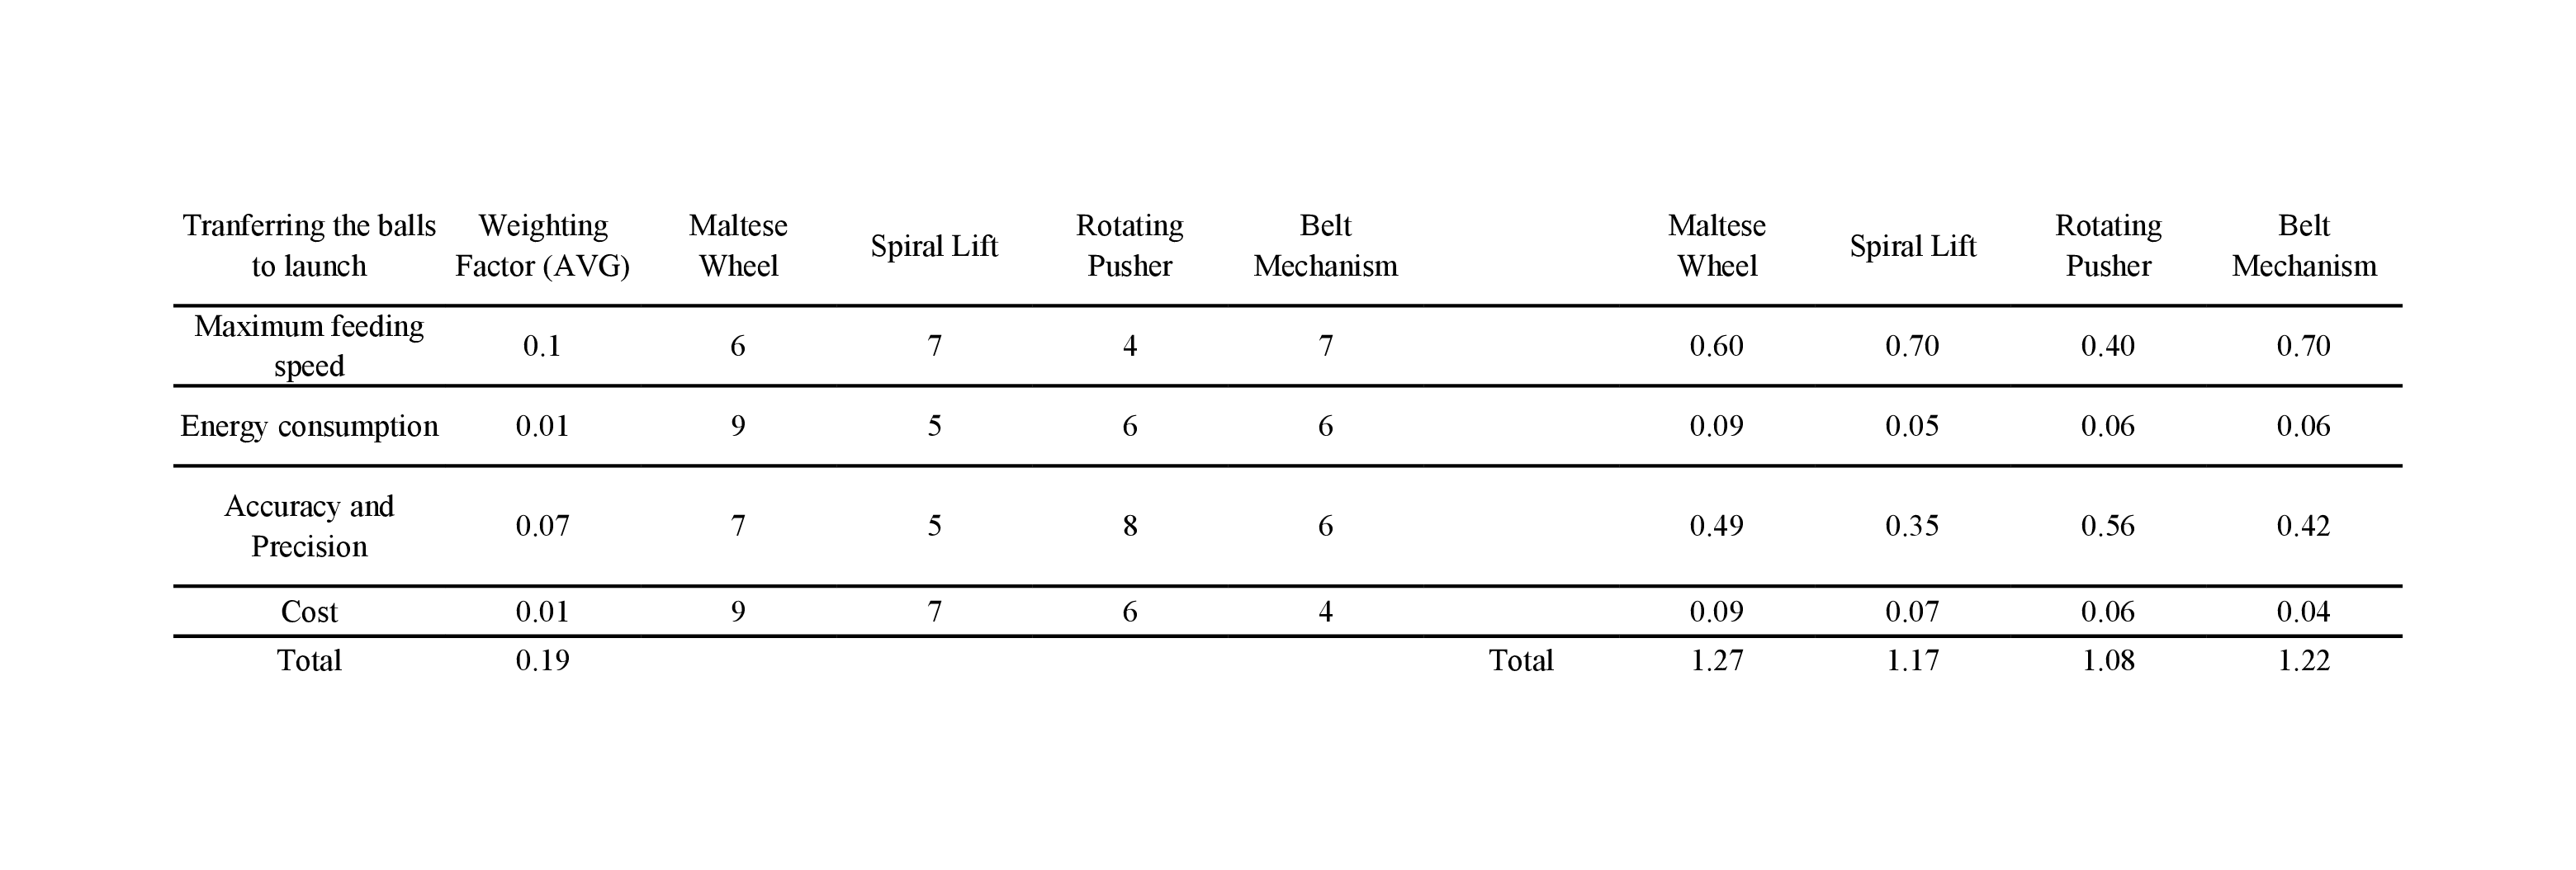
\includegraphics[width=1\textwidth]{Decision matrices/transfer to launch.png}
    \caption{Transferring the balls to launch }
\end{figure}

For controlling the ball feed for launching, three alternatives were considered. As was the case with ball feed control for storage, the stepper motor was identified as the optimal solution. It was selected as the optimal choice due to its overall performance, which satisfied expectations across all criteria.

\begin{figure}[H]
    \centering
    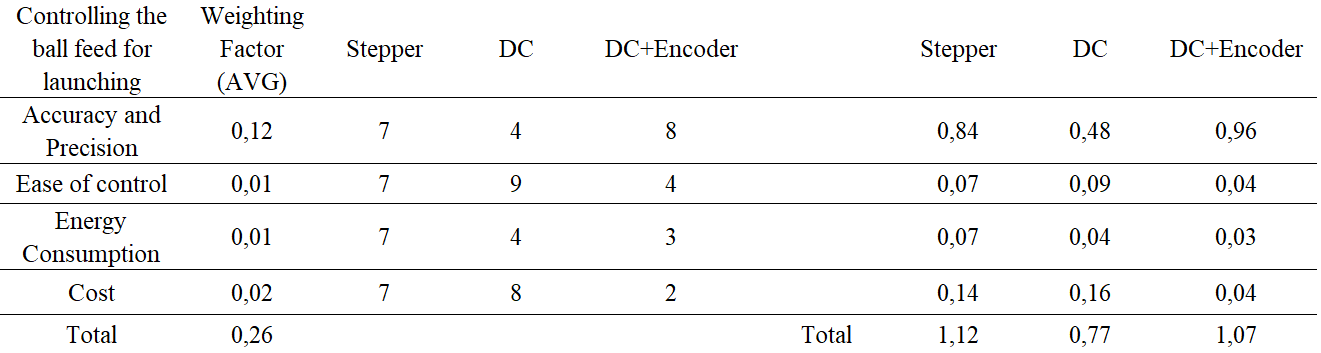
\includegraphics[width=1\textwidth]{Decision matrices/controlling ball feed for launching.png}
    \caption{Controlling the ball feed for launching}
\end{figure}

For the subfunction of giving the balls the desired frequency, six alternatives were considered. While the rotating pusher was identified as the optimal solution based on the decision matrix, particularly excelling in meeting the maximum attainable serving frequency criterion, the overall system design and integration with other subfunctions favored the use of the Maltese wheel. This approach ensures better compatibility and efficiency in the final design.

\begin{figure}[H]
    \centering
    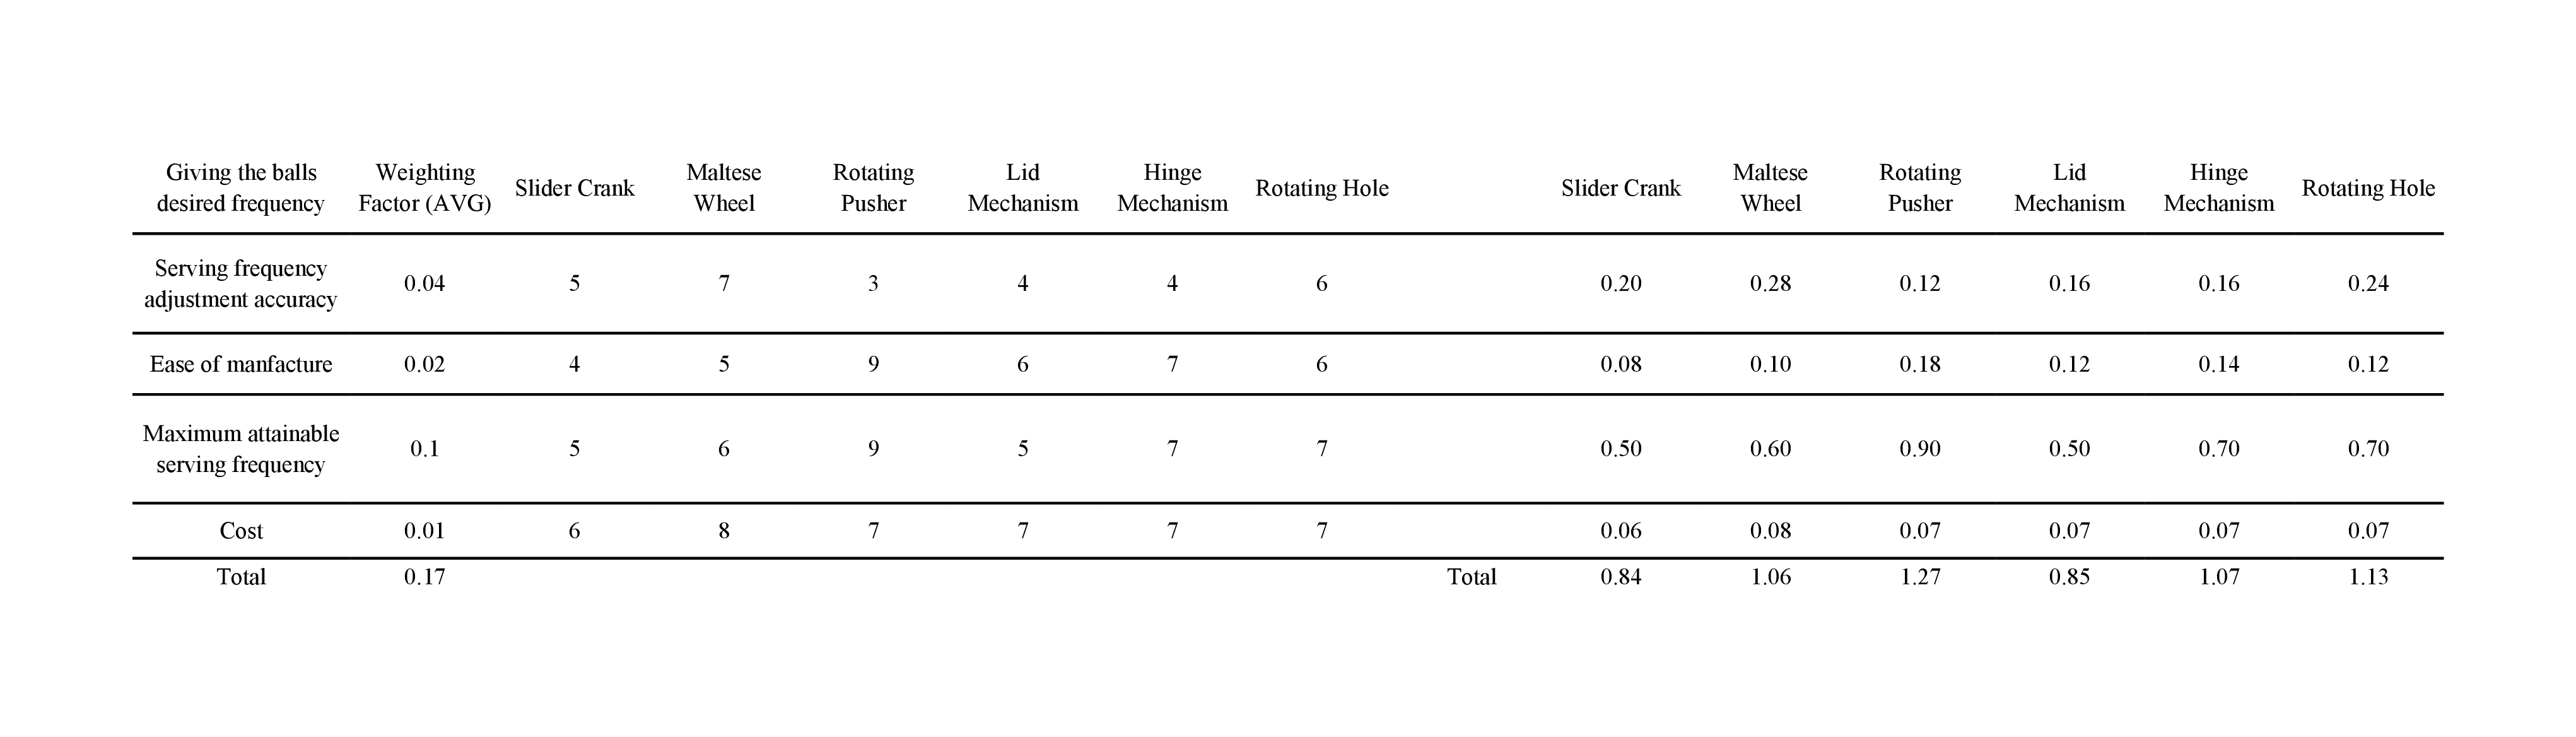
\includegraphics[width=1\textwidth]{Decision matrices/give frequency.png}
    \caption{ Giving the balls desired frequency}
\end{figure}

For the subfunction of controlling the ball frequency, three alternatives were evaluated. According to the decision matrix evaluation, the stepper motor was determined to be the optimal solution due to its better performance in terms of accuracy, precision, and cost-effectiveness, making it the most suitable choice for this application.

\begin{figure}[H]
    \centering
    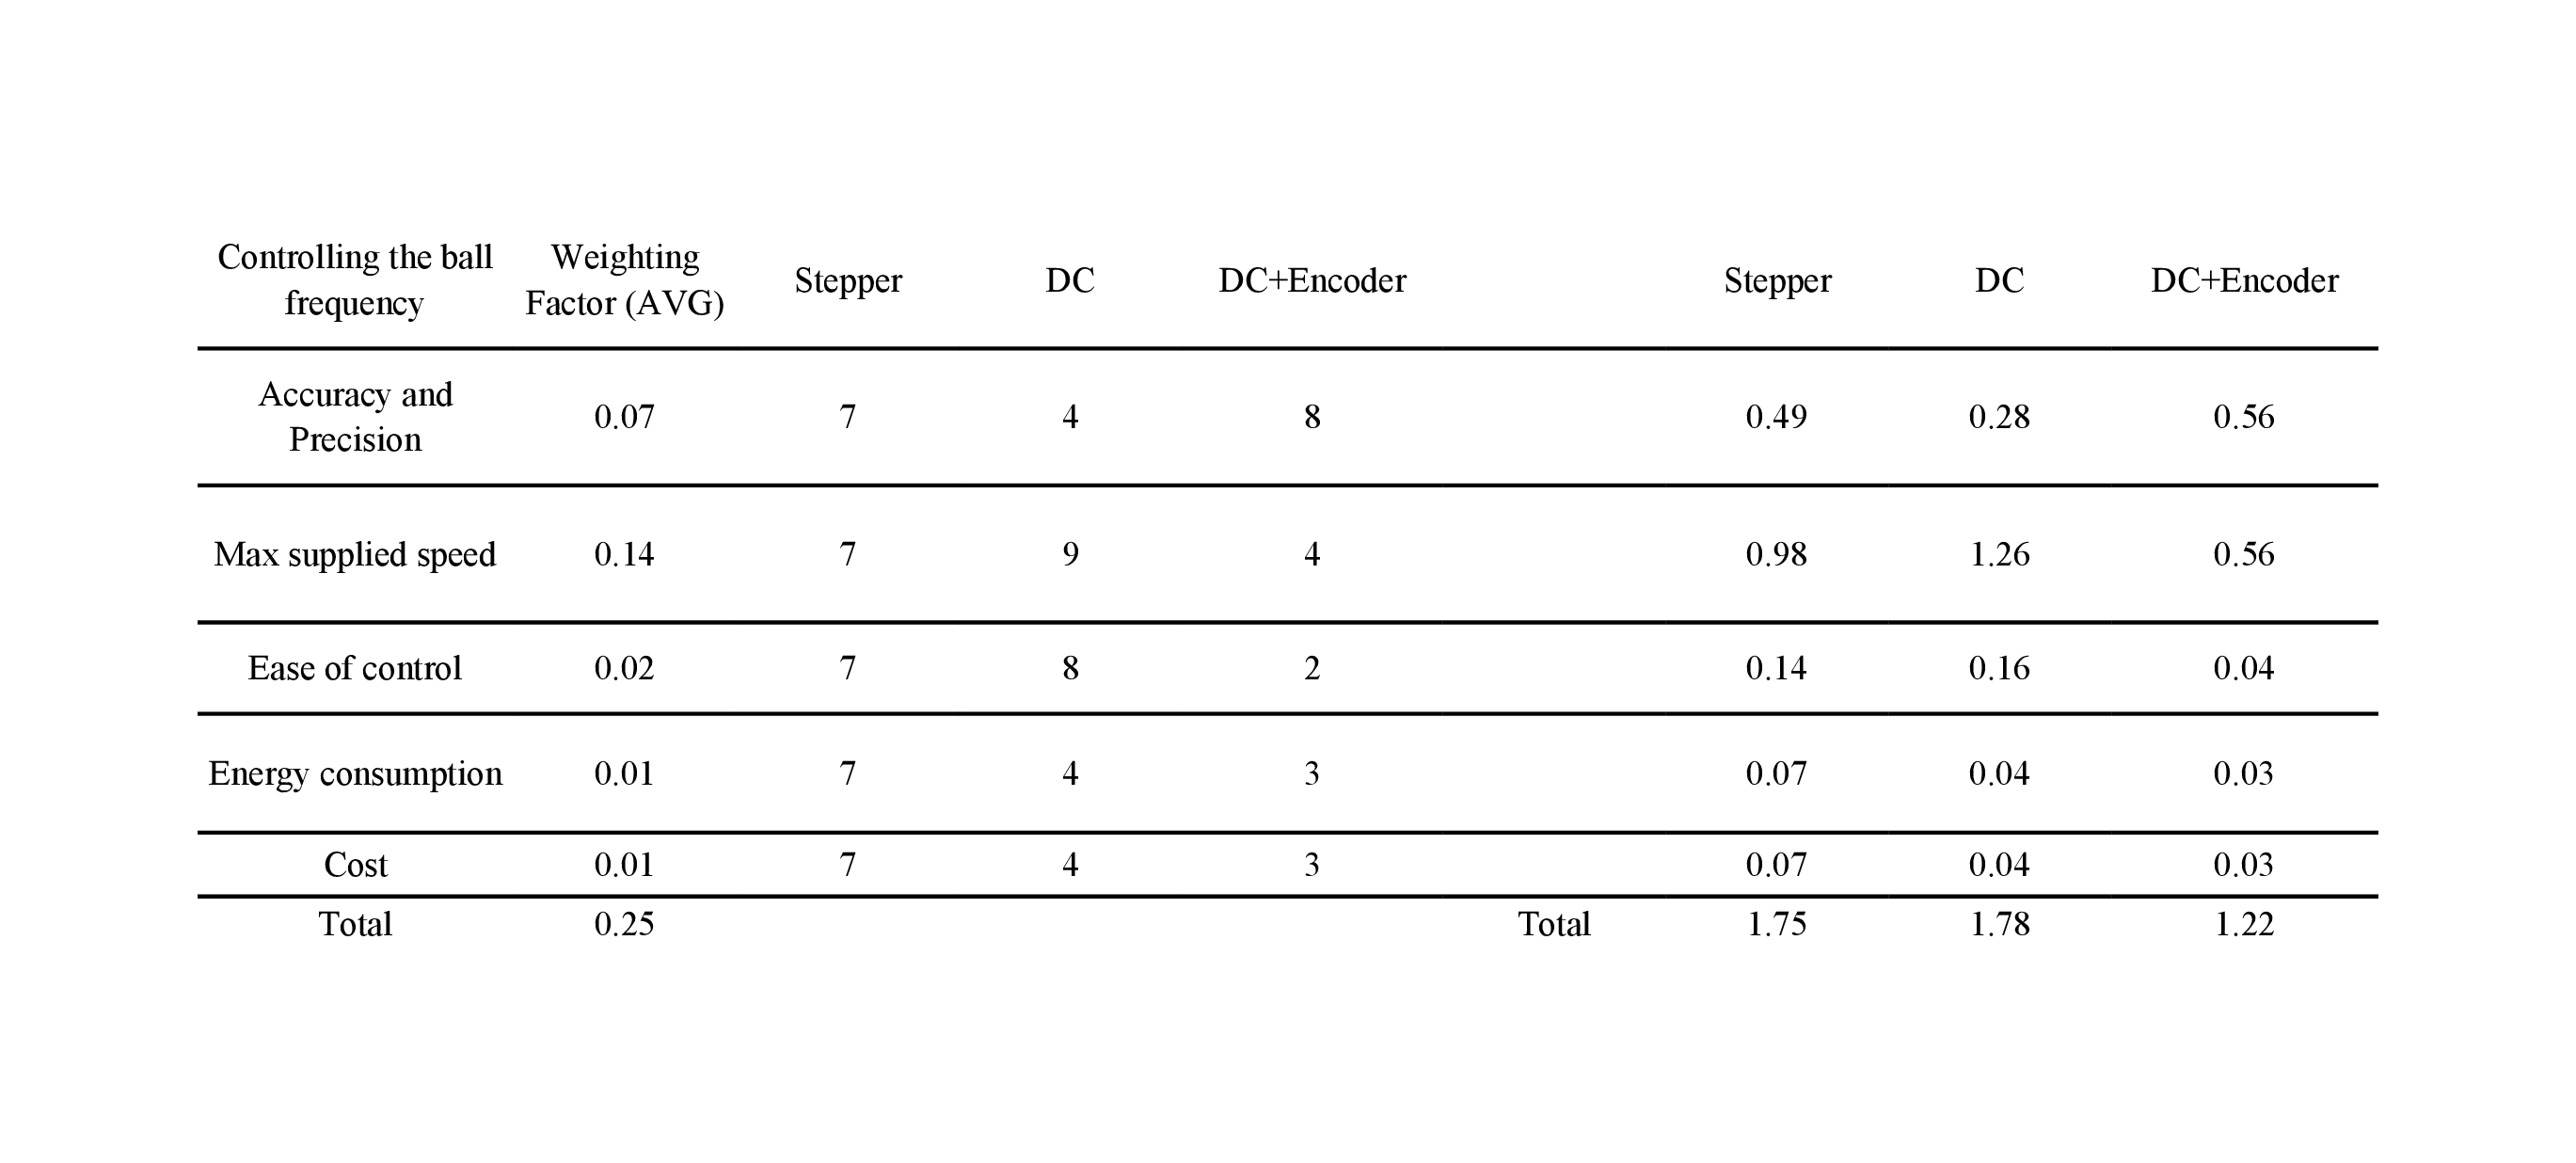
\includegraphics[width=1\textwidth]{Decision matrices/control frequency.png}
    \caption{Controlling the ball frequency}
\end{figure}


\begin{figure}[H]
    \centering
    \rotatebox{90}{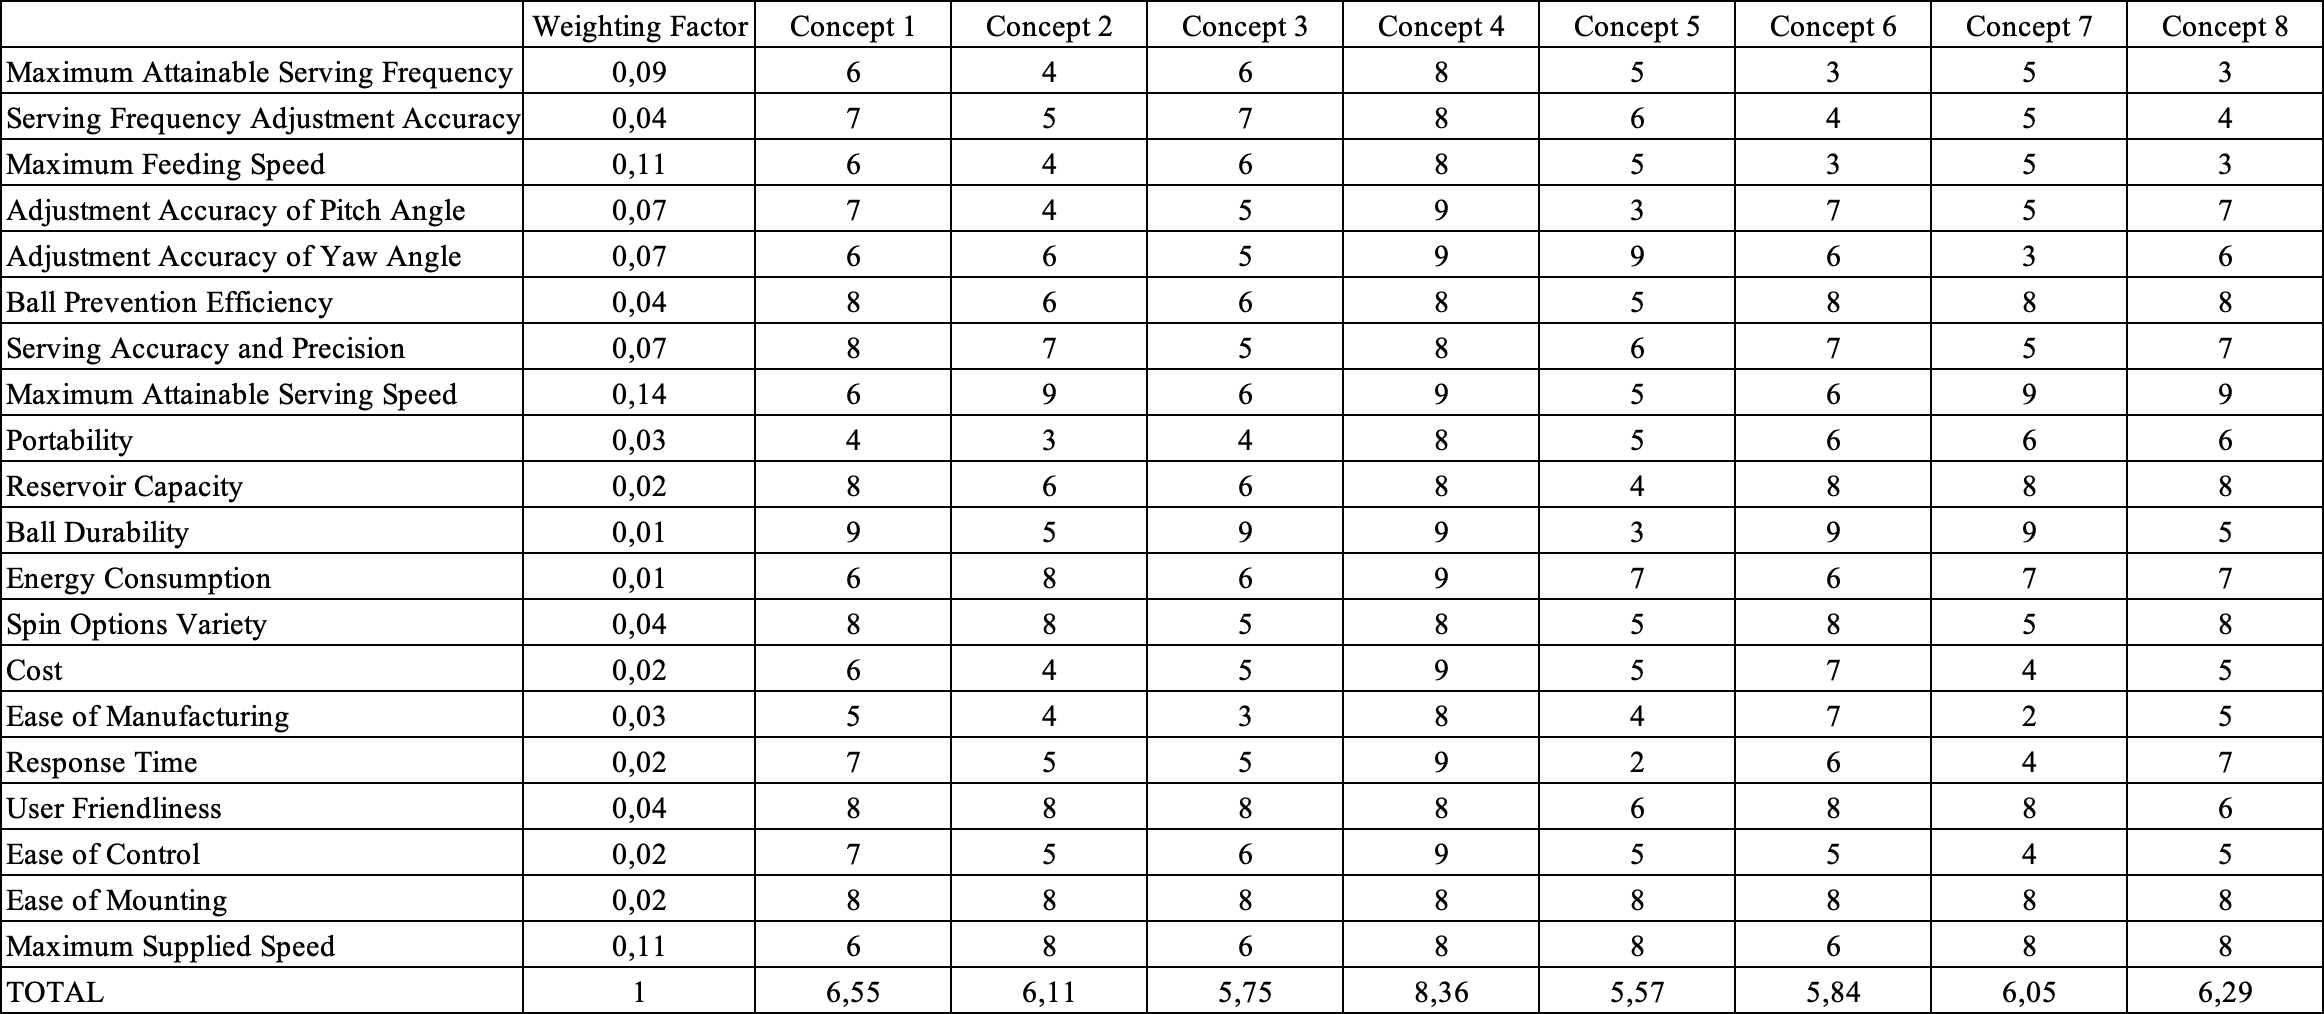
\includegraphics[width=\textheight]{obaa.jpg}}
    \caption{Concept Evaluation Normalized\cite{statista2024}}
    \label{fig:wholesales}
\end{figure}

\section{Best Concept}

\begin{minipage}{0.7\textwidth}

The best concept is chosen as Concept 4. Several factors determine this choice. Balls are stored in a groove structure (Figure ~\ref{fig:groove_mechanism}), ensuring organized storage and smooth feeding into the system. A net mechanism (Figure ~\ref{fig:net}) collects balls post-use and channels them back to the storage area, promoting recyclability and sustainability, enabling the user to have a continuous and favorable training experience. Possible ball leakage is prevented by using a net system to catch the balls and a groove mechanism for storage.

The balls are transferred from the storage to the launcher by a Maltese wheel (Figure ~\ref{fig:maltese}) through the "pushing effect" of consecutive balls, ensuring a smooth and consistent supply to the launcher. This Maltese wheel, operated by a stepper motor, facilitates precise ball direction toward the launch mechanism. The desired ball frequency is achieved by the rotation of the Maltese wheel, which determines the number of balls transferred per unit of time.

After the transfer process, a 3-wheel mechanism (Figure ~\ref{fig:3wheel}) launches the balls with the desired speed and spin. The speed is controlled by the linear speed of the wheels, which are driven by BLDC motors. For instance, if all three wheels rotate at the same speed (assuming equal dimensions), the ball is launched without spin. Conversely, a speed difference between the wheels imparts spin to the ball, such as top-spin, side-spin, or back-spin, depending on the faster wheel(s). Thus, the spin is determined by the relative angular speeds of the wheels.

The trajectory (yaw and pitch angles) of the launched ball is adjusted by gears (Figures ~\ref{fig:gear} and ~\ref{fig:gear2}), controlled by servo motors. The yaw angle is set by rotating the base, and the pitch angle is adjusted by rotating the launching head. Users can input frequency and trajectory settings via an integrated controller (Figure ~\ref{fig:integrated} ) equipped with a potentiometer and buttons (Figure ~\ref{fig:pot}) for numerical adjustments. These components simplify configuration and provide a user-friendly experience.

Finally, the system is secured to the table using clamps (Figure ~\ref{fig:clamp}) to prevent unwanted movements during training sessions.
\end{minipage}%
\hfill
\begin{minipage}[t]{0.25\textwidth}
    \centering
    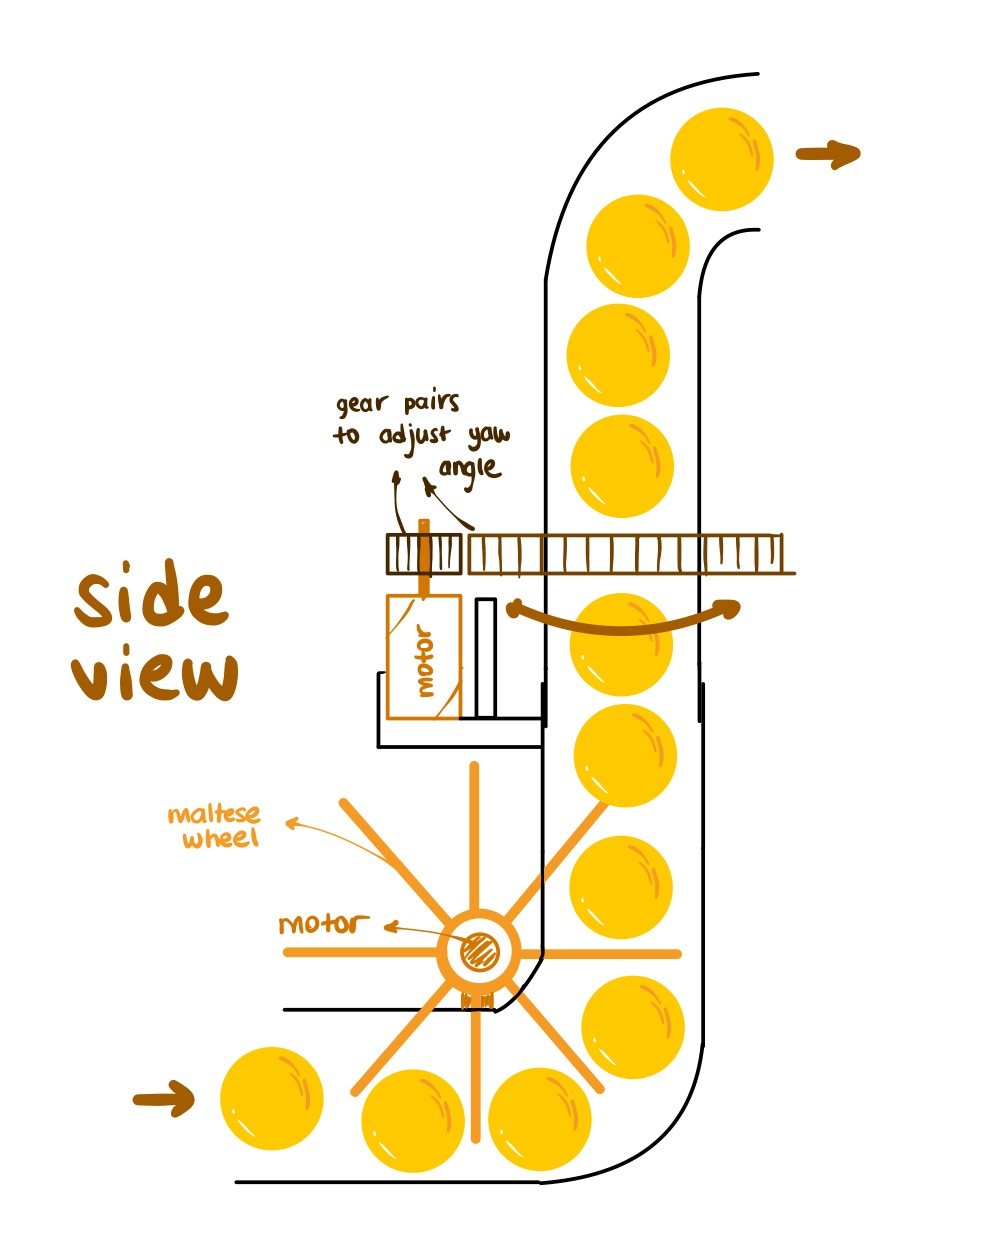
\includegraphics[width=\textwidth]{best_concept/side_feeder.jpeg}
    \captionof{figure}{Feeder side view}
    \vspace{1em}
    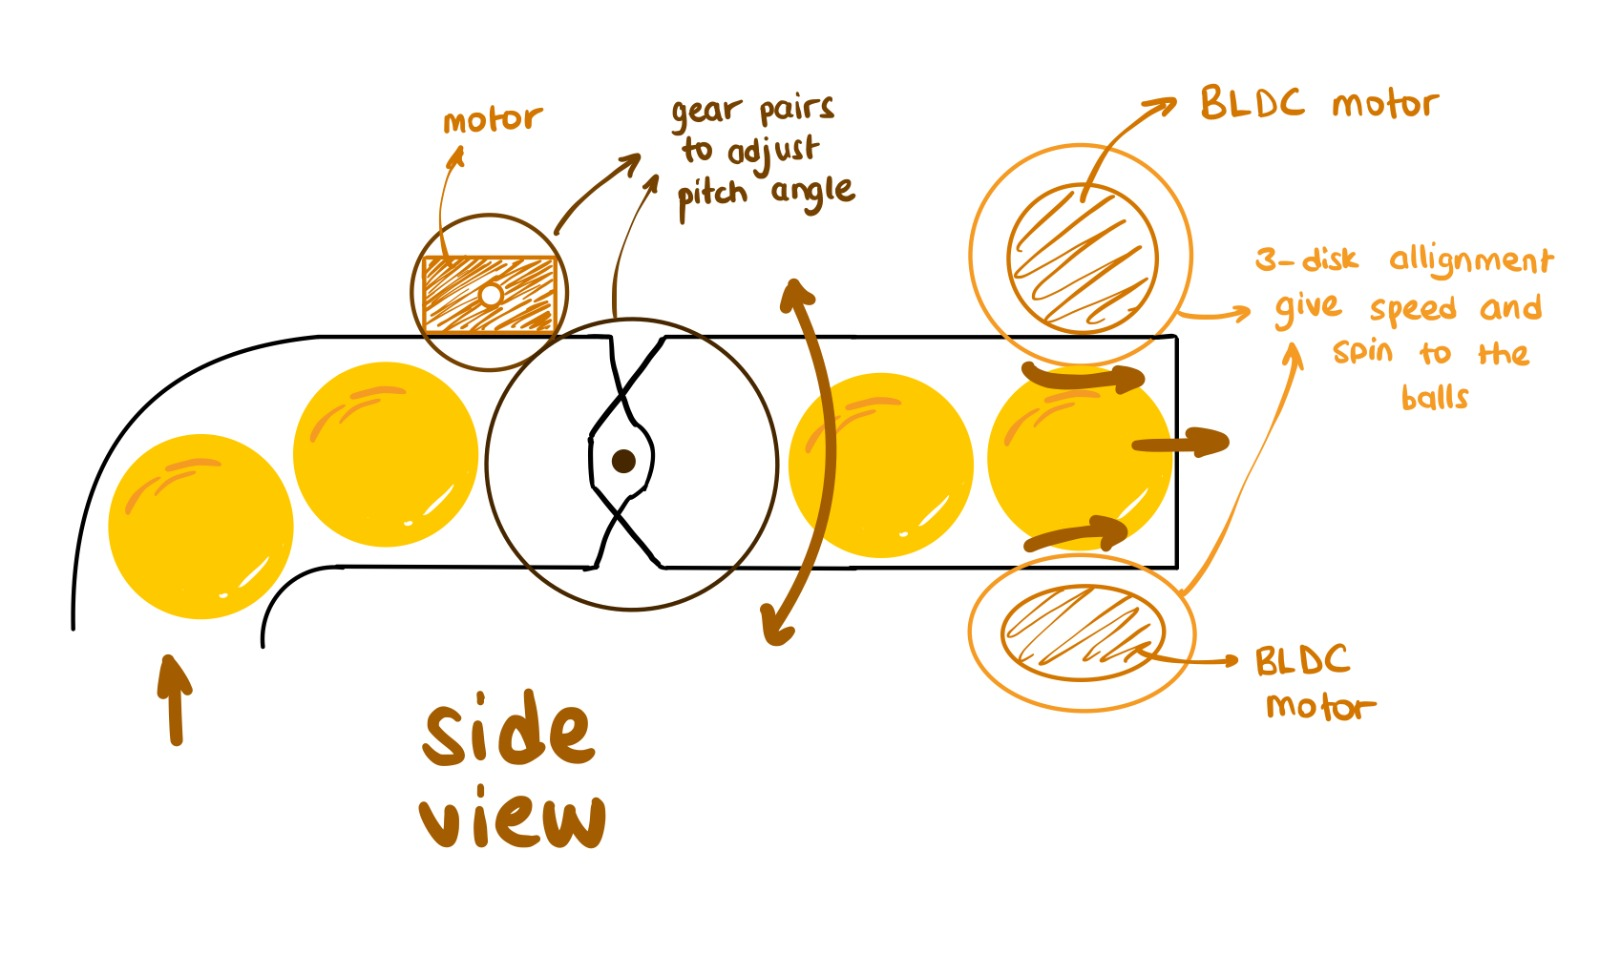
\includegraphics[width=0.9\textwidth]{best_concept/side.jpeg}
    \captionof{figure}{Side view}
    \vspace{1em}
    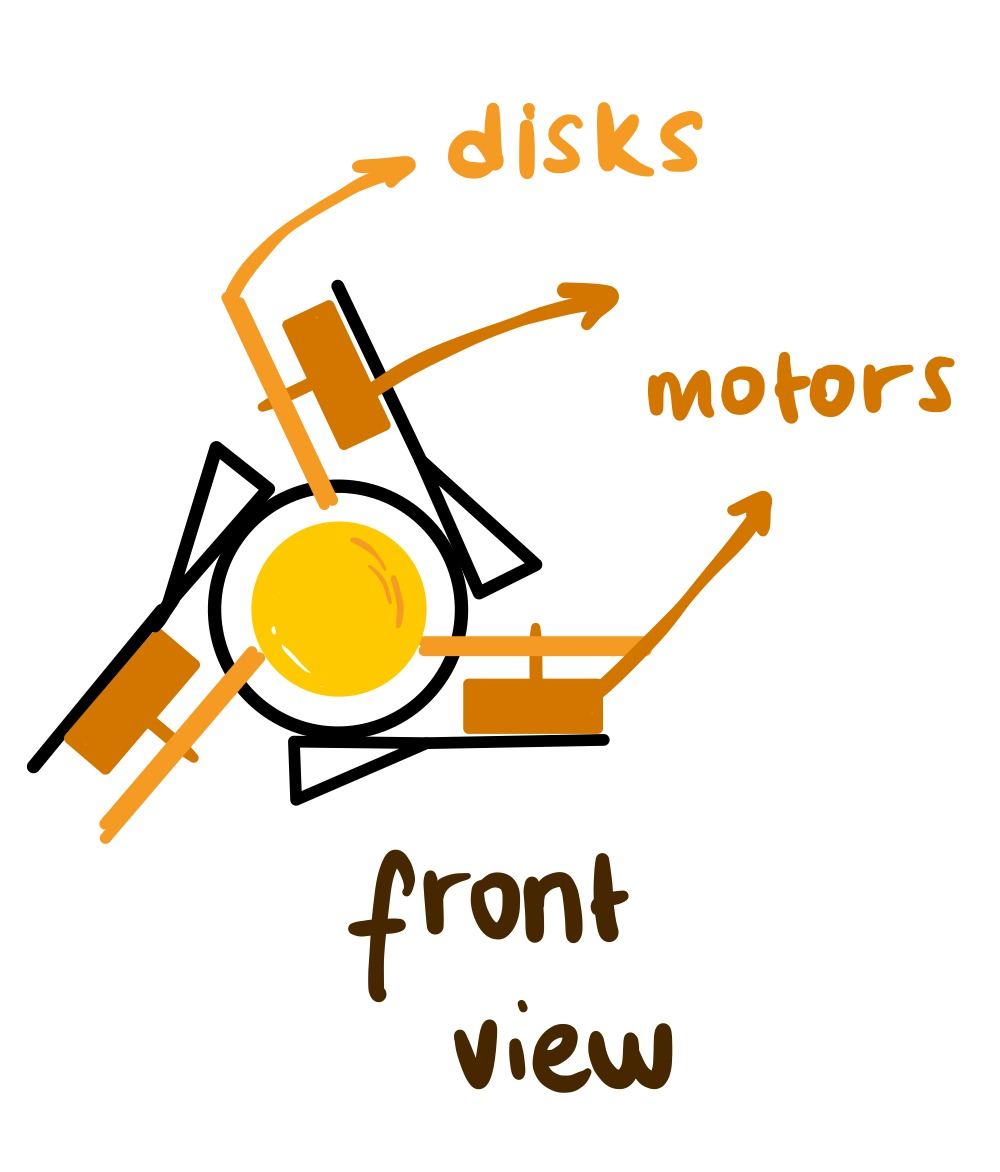
\includegraphics[width=0.5\textwidth]{best_concept/front.jpeg}
    \captionof{figure}{Front View}
\end{minipage}


\begin{figure}[H]
    \centering
    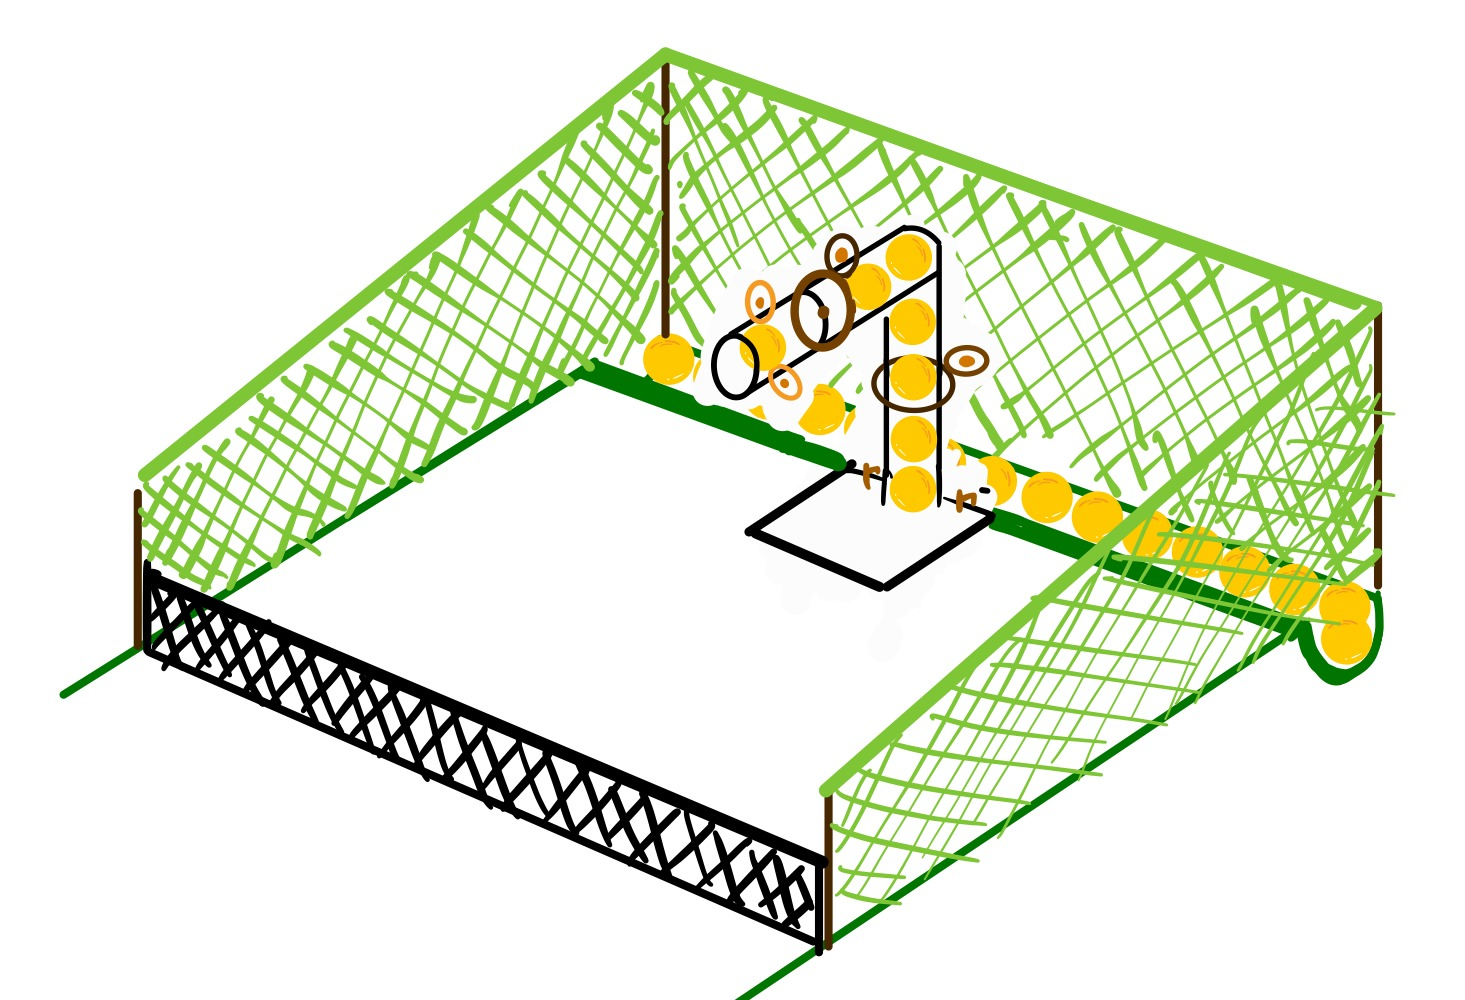
\includegraphics[width=0.5\textwidth]{best_concept/whole.jpeg}
    \caption{Orthogonal view}
    \label{fig:whole_best}
\end{figure}


\section{Summary and Conclusion}

In this report, development of the conceptual design of the project of a Table Tennis Ball Pitcher Machine is presented. The sub-function concepts listed in the Morphological Chart created in the previous steps of the project are evaluated according to the relevant design criteria, and decision matrices are created for each to decide on the most viable options. Then, from these sub-functions, eight different overall concepts are developed by using the combination of different ideas together and observing how the different mechanisms complement each other so as to create the best functional alternatives for the task. What is next is to then evaluate these eight concepts with the overall design criteria to choose the best concept among them. This approach ensures that the concept chosen to proceed with the project brings the most efficient and effective solutions to project requirements, and is the best selection compared to the other alternatives brought up.

\chapter{Detailed Design}

\section{Introduction}

This report encapsulates the finalized decisions and selections; procedures and calculations carried out for the detailed design of the Automatic Table Tennis Ball Pitcher Machine Project. The operating principle of the system, how the system differs from the similar available products on the market, calculations for the functions and the analysis of the system, control algorithms, optimization, manufacturing methods, sustainability analysis, test plans to be carried out, and finally performance analysis and discussion will be laid out clearly. It is important that every one of these steps are documented in detail so that the system is easily and fully understood for any future referencing.

\section{Properties of Designed System}

In this part, properties of the final design will be laid out clearly, where each sub-function will be explained, and the overall operating principle of the system will be given. Important aspects of the design will be discussed, where the applications and functions of the system that differs it from the existing products on the market will be mentioned. Finally, for this part, the machine elements of the system will be considered, and the requirements they bring will be reported.

\subsection{Operating Principle}

The balls are directed to the feeding section from the groove with the help of a channel. The frequency of the balls in the feeding section is adjusted by a Maltese wheel and redirected to the launcher. This Maltese wheel is capable of providing a frequency of up to 60 balls per minute to the system. The system contains a gear pair to adjust the yaw angle and a motor to control the gear pair. These gears are located in a box with bearings enabling the vertical position of the pipe attached to the neck. On the launcher, there is a gear pair controlling the pitch angle, and the motor controlling this gear pair.
This part enables unconstrained movement since it consists of two parts connected by a pin. Finally, the balls reaching the end of the launching part are launched by a 3-wheel system with the desired speed and spin options.  After the launch, the balls are recycled (if they are in the expected region) by a 1 meter high net, back to the storage.  
The device is controlled with an integrated controller and by the potentiometer with buttons located on the controller, the spin, frequency, speed, pitch and yaw angle values are controlled. The device is to be fixed to the table by clamps, and should be stabilized in case of any vibration.

\subsection{Important Aspects of Design}

Although the market for a table tennis ball pitcher machine is not as abundant as some other electronic devices, there are some different designs readily available. The project at hand has to offer some improvements and variations to the existent ideas so it can be marketed as a unique product. 
During a literature survey and market research, it was observed that most commercial products use a rotating head design for launch functions. While this design indeed allows for giving spin to the balls, it also limits how fast the mechanism can switch between different spins, as it requires the head to make a turn beforehand. The design idea in this project utilizes a 3-wheel system for giving the spin, which allows for quicker transition between different spins, ergo allowing for higher frequency.
During the tests, it was found that the wheels attached to the motors for launching are the parts most prone to damage, due to friction and wear during launch. In the design for this project, replacement of the wheels has been facilitated so as to allow for a longer service life, which is an option that has not been come across in any of the other commercial products surveyed.
One limitation the project has is it is fixed at one point on the table. Although it is not a common function in most commercial products, there are some designs that implement flexible movement, so this can be pointed out as a shortcoming compared to those products.

\subsection{Machine Elements and Functional Requirements}

The selection of machine elements is carried out by dividing the entire assembly into smaller subassemblies. Within each subassembly, the choice of machine elements is guided by specific functional requirements, such as ability to withstand loads, accommodate forces, or fit within geometric constraints. This approach ensures that each machine element is selected to meet the demands of its role in the overall design, resulting in effective assembly.


\subsubsection{Launcher}

In the launcher assembly, two socket head screws are used for each motor, totaling six screws. Since these screws are not subjected to any radial load and experience minimal preload, only geometric requirements were considered during their selection. The selected screws are standard M4 socket head screws with a length of 7 mm, chosen according to standard specifications. The design of the launcher is very light-weight and material usage is optimized compared to common products. This is due to using 3 wheel configuration which is controlled with 3 BLDC motors. Without rotating the head part, alternating the speeds of the 3 disks we can give any spin at a desired angle.

\begin{figure}[h!]
    \centering
    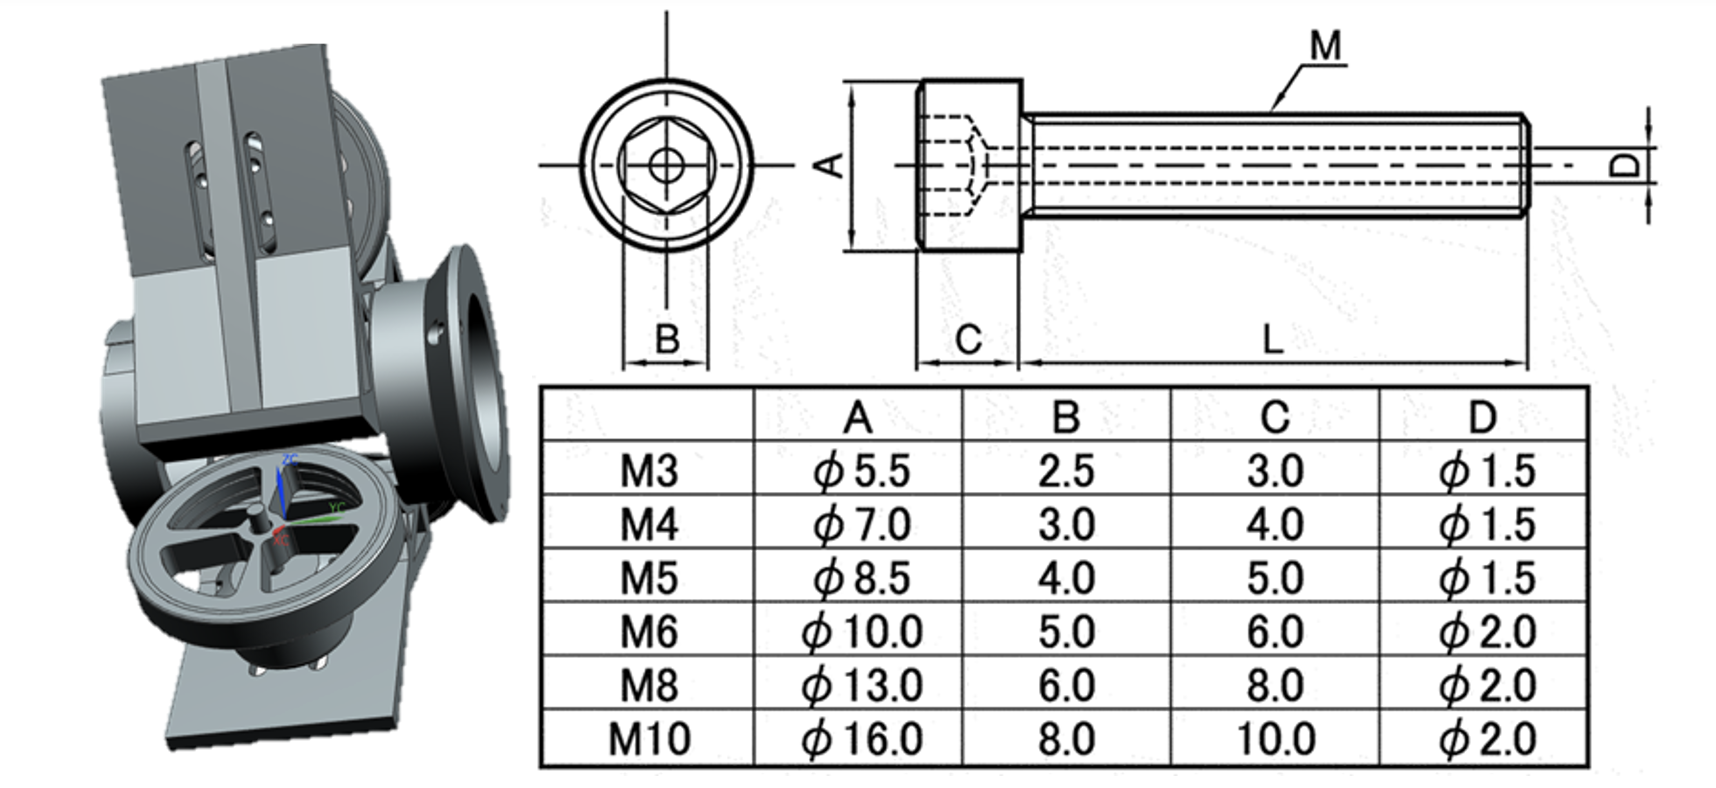
\includegraphics[width=0.7\linewidth]{2.3.1.png}
    \caption{Launcher Subassembly}
    \label{fig:enter-label}
\end{figure}

\subsubsection{Pitch Angle}

The pitch angle subassembly is secured to the launcher using three M3 screws with nuts, each 13 mm in length. For attaching the pitch motor to the pitch angle subassembly, two M3 hex bolts (13 mm) with three nuts are used. To connect the pitch angle subassembly to the main body, four M4 hex bolts (13 mm) with corresponding nuts are utilized. Additionally, the pinion has 17 teeth, while the gear has 65 teeth.

\begin{figure}[h!]
    \centering
    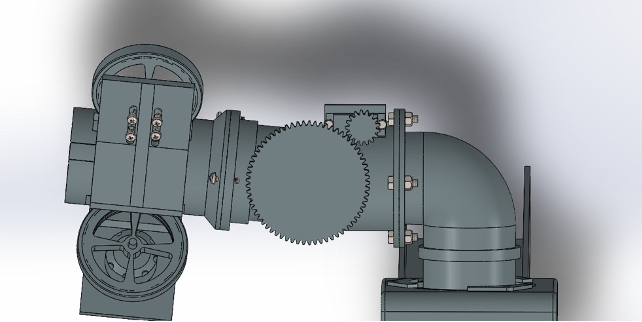
\includegraphics[width=0.7\linewidth]{2.3.2.png}
    \caption{Pitch angle subassembly}
    \label{fig:enter-label}
\end{figure}


\subsubsection{Main Body and Yaw Angle}

The yaw angle assembly in the table tennis ball pitching machine is designed for precise motion control, achieved using a gear pair and bearings. Two SKF 6810 bearings are incorporated based on calculated radial and axial force requirements, ensuring smooth rotation and durability. The bearings are mounted within blind holes in the housing, secured using hex-head M4 screws. Threaded inserts and hex-head screws fasten the main body components.
The assembly integrates a bushing with keys for coupling the driven gear, which includes corresponding keyways to prevent slippage. A servo motor drives this setup, providing precise angular adjustments and smooth acceleration. A 0.45 gear ratio is selected to enhance yaw angle control accuracy.
This design rotates the system's feeding line rather than the launcher head directly, offering multiple advantages:

\begin{enumerate}
    \item Compact launcher design.
    \item Reduced stress on the launcher components.
    \item Simplified assembly and disassembly.
\end{enumerate}

The spur gear pair minimizes axial load, while the feeding line, shrink-fitted into two bearings at either end of the main body, ensures optimized reliability. The upper part of the feeding system is isolated from the pipe, ensuring only the top section rotates, which requires the launcher components to remain lightweight for efficient operation.

\begin{figure}[h!]
    \centering
    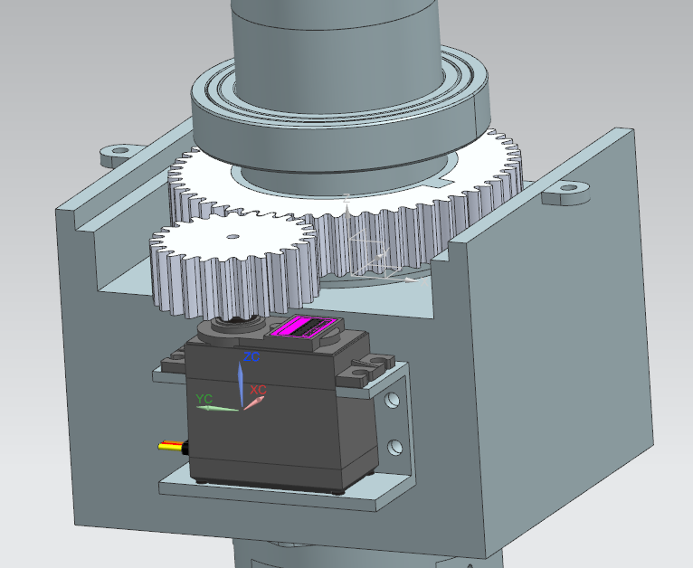
\includegraphics[width=0.5\linewidth]{2.3.3.1.png}
    \caption{Yaw angle subassembly}
    \label{fig:enter-label}
\end{figure}

\begin{figure}[h!]
    \centering
    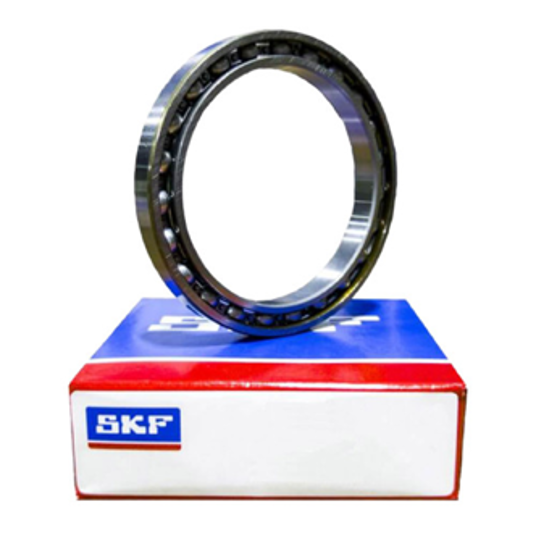
\includegraphics[width=0.3\linewidth]{2.3.3.2.png}
    \caption{6810 ZZ Bearing}
    \label{fig:enter-label}
\end{figure}

\begin{table}[h!]
\scriptsize
\centering
\caption{Yaw angle components}
\begin{tabular}{|c|p{9cm}|}
\hline
\textbf{Component} & \textbf{Properties} \\ \hline
Driving Gear & Spur Gear, Module 1.5, Teeth Number 25 \\ \hline
Driven Gear & Spur Gear, Module 1.5, Teeth Number 55, Keyway slotted \\ \hline
Motor & MG996R Servo Motor \\ \hline
Bushing & Manufactured with keys, Shrink fit \\ \hline
Bearings & NSK 6910 ZZ Ball Bearing, High load and fatigue capacity, Shrink fit \\ \hline
Feeding Line & 50mm diameter pipe, Shrink fit \\ \hline
\end{tabular}
\label{table:yaw_components}
\end{table}


\subsubsection{Feeding Mechanism}
The feeding mechanism incorporates a Maltese wheel designed for continuous ball delivery to the launcher. The wheel is driven by a stepper motor, with each 60-degree rotation feeding one ball. This setup allows precise control over the number of balls to be launched.
The feeding pipe is tightly secured to the feeding holder using an H6/e6 interference fit. The connection is further reinforced with four M3 set screws, each 3 mm in length, a method commonly used in prosthetic applications for its reliability. The feeding holder is attached to the main body using M4 bolts and threaded inserts, providing a factor of safety of approximately 3.8.
This design is highly compatible with the ball recycling system, ensuring efficient operation. However, a notable drawback is the increased space requirement for the feeding pipe.

\begin{figure}[h!]
    \centering
    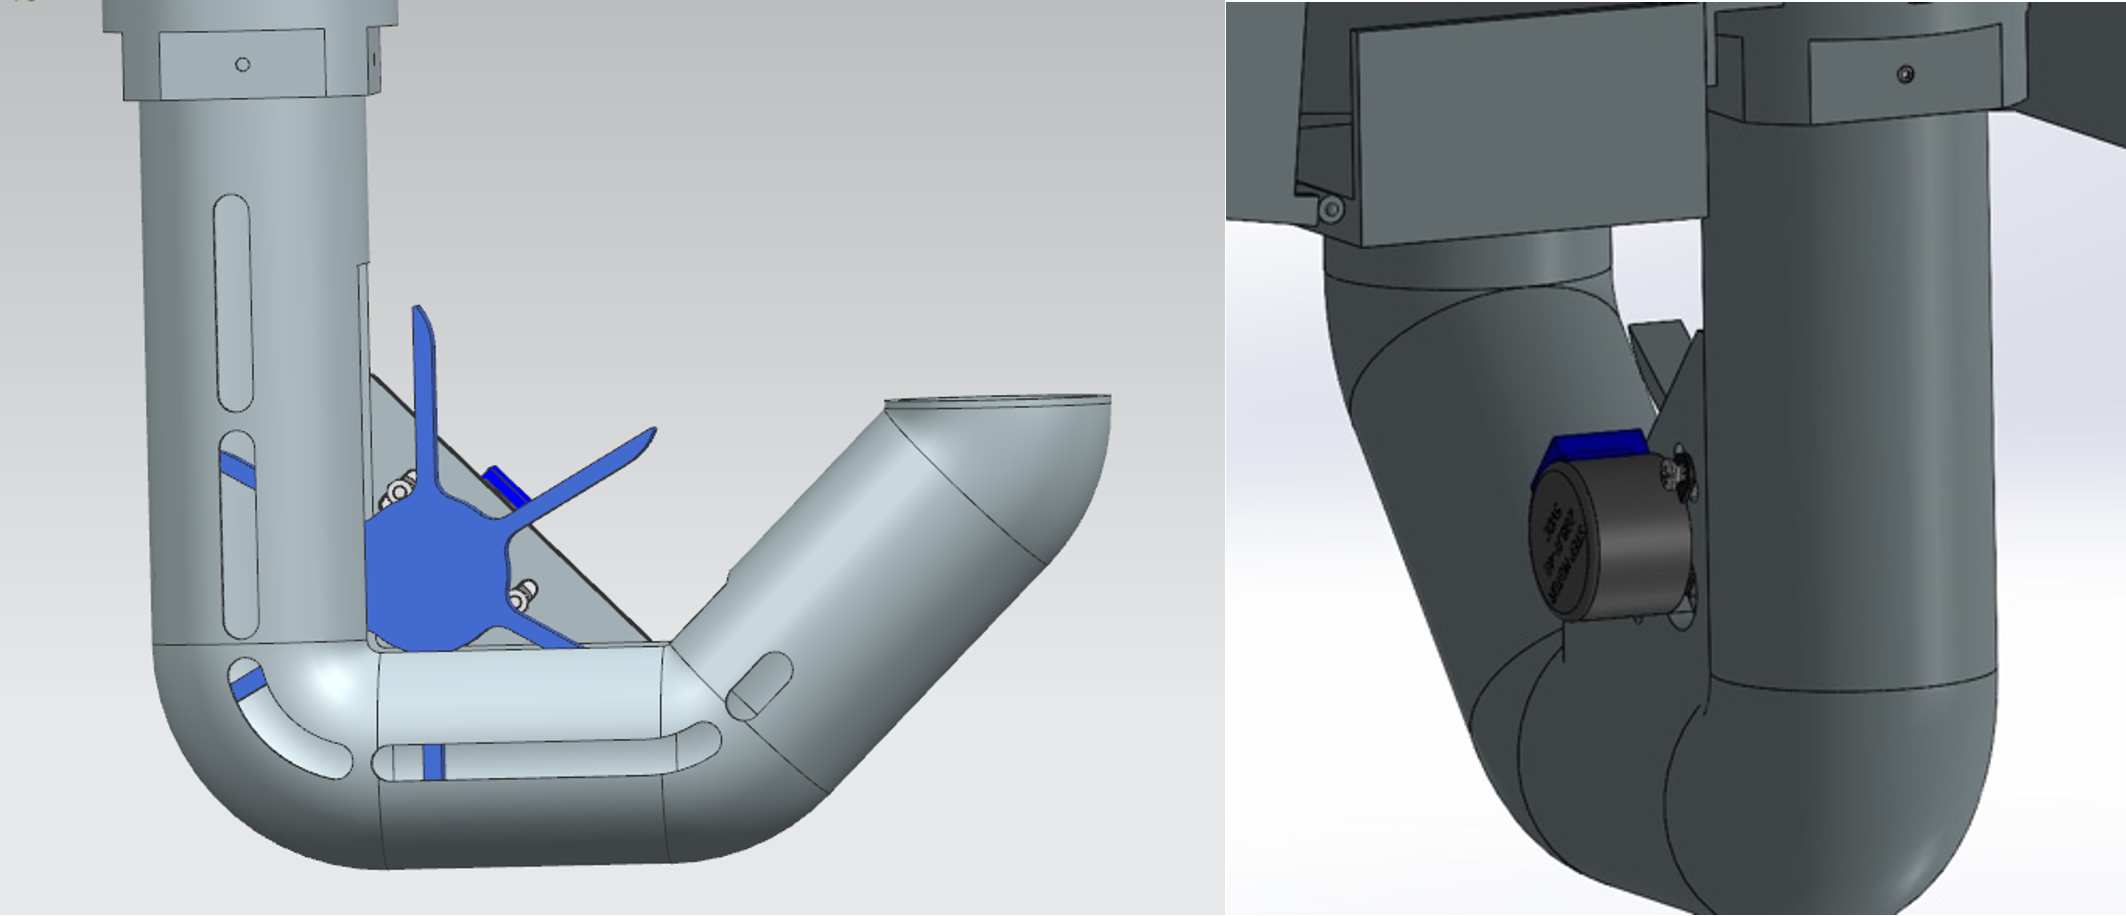
\includegraphics[width=0.7\linewidth]{2.3.4.1.png}
    \caption{Feeding system subassembly}
    \label{fig:enter-label}
\end{figure}

\begin{figure}[h!]
    \centering
    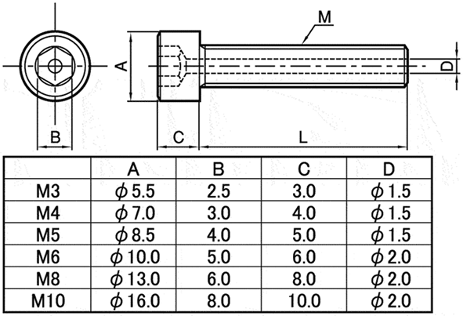
\includegraphics[width=0.5\linewidth]{2.3.4.2.png}
    \caption{Socket head bolt}
    \label{fig:enter-label}
\end{figure}

\begin{figure}[h!]
    \centering
    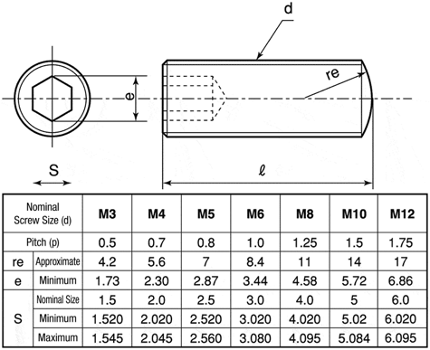
\includegraphics[width=0.5\linewidth]{2.3.4.3.png}
    \caption{Set screw}
    \label{fig:enter-label}
\end{figure}

\begin{table}[h!]
\scriptsize
\centering
\caption{Feeding system components}
\begin{tabular}{|c|p{6cm}|}
\hline
\textbf{Component} & \textbf{Properties} \\ \hline
Maltese Wheel & 6 slots, ABS \\ \hline
Pipe & 50 mm outside diameter ABS \\ \hline
Motor & Nema17 Step Motor \\ \hline
Bolts and Nuts & M4, Stainless Steel \\ \hline
Set Screws & 3mm length, Nylon tip, Alloy Steel \\ \hline
\end{tabular}
\label{table:feeding_components}
\end{table}


\subsubsection{Ball Recyclability}

A net is used to catch the balls and is complemented by grooves attached to both sides of the robot. The net directs the caught balls into the grooves, allowing them to roll down into the storage unit. The grooves serve as guides, ensuring the balls are efficiently funneled into the storage area. The net is securely connected to the grooves and anchored to the table for stability.

\begin{figure}[h!]
    \centering
    \includegraphics[width=0.5\linewidth]{2.3.5.1.png}
    \caption{Ball Recyclability system}
    \label{fig:enter-label}
\end{figure}

\subsubsection{Storage and Groove}

The grooves are attached to the storage unit using hinges, allowing them to fold for enhanced portability. The connection between the storage unit and the grooves is achieved with welded hinges, as illustrated in the accompanying figure. To secure the storage unit to the main body, four L-plates are utilized. These plates are fastened using M4 bolts (13 mm in length) and nuts, ensuring a stable and reliable connection.

\begin{figure}[h!]
    \centering
    \includegraphics[width=0.5\linewidth]{2.3.6.1.png}
    \caption{Storage system subassembly}
    \label{fig:enter-label}
\end{figure}

\subsubsection{Mounting}

The clamp is specifically designed to support the entire weight of the system. Calculations indicate that the primary factor influencing clamp performance is not the system's weight but the pretension of the clamping screw. To ensure secure attachment, the minimum clamping distance is set to 18 mm, matching the thickness of a standard table.
The clamp is connected to the main body using M5 steel bolts and brass threaded inserts, chosen for their availability and chemical compatibility. To optimize load distribution and stability, four bolts are arranged in a rectangular pattern, providing a firm and reliable fixation.

\begin{figure}[H]
    \centering
    \includegraphics[width=0.3\linewidth]{2.3.7.1.png}
    \caption{Clamp}
    \label{fig:enter-label}
\end{figure}


\section{Engineering Calculations}

This section outlines the essential engineering calculations for the Table Tennis Ball Pitcher Machine, covering areas such as material strength, kinematics, dynamics, and force analysis. Assumptions, modeling simplifications, and approximations are clearly stated to ensure clarity and precision. The calculations validate the performance, safety, and reliability of the design, ensuring it meets the specified requirements. 
The calculations and design decisions can be divided into two main parts:

\subsection{Decisions based on meeting the performance criteria target}

In that section, the decisions based on meeting the performance criteria targets are presented. The type of modelling, the related component of the system, the design parameters to be decided, and the explanations including the assumptions and approximations, the methods or any aid of commercial software are explained in detail.

The table shows the planned models, analyses, and tests to ensure the system meets the required performance standards. For each part or subsystem, it describes the modeling type (analytical, numerical, or experimental), important design factors, and key methods used. It also explains assumptions, like slip percentage and operating conditions, and lists tools such as MATLAB/Simulink, Siemens NX, and Python for simulations and optimization. Table includes motor torque and speed modeling, control strategy simulations, optimizing disk dimensions, and testing materials for the launcher. 

\begin{table}[H]
\centering
\caption{Decisions based on meeting the performance criteria target (Part 1)}
\scriptsize % Reduced font size for the entire table
\renewcommand{\arraystretch}{1.5}
\setlength{\tabcolsep}{4pt}
\begin{tabular}{|>{\raggedright\arraybackslash}p{3cm}|>{\raggedright\arraybackslash}p{3cm}|>{\raggedright\arraybackslash}p{3cm}|>{\raggedright\arraybackslash}p{6cm}|}
\hline
\textbf{Analytical Modelling / Numerical Modelling / Numerical Experiment / Physical Experiment} & \textbf{Component / Subsystem / Whole System} & \textbf{Design Parameters to be Decided} & \textbf{Explanation (State assumptions, any commercial software for the implementation, and details of methods like DoE, optimization etc.)} \\ \hline
Numerical Modelling & Launch Motors & Motor Type, Torque, Speed & Torque and speed requirements for launching wheels will be calculated to achieve a maximum ball speed of 30 m/s. Also, a simulation in Python can be used to model motor torque, angular speed, and efficiency based on required ball velocities and spin. The assumed slip is 20\%. \\ \hline
Numerical Experiment & Launch Motors & Motor Control Strategy & Motor response and speed control for spin adjustments will be simulated. BLDC/DC motors will be controlled via Pulse Width Modulation (PWM) using MATLAB/Simulink for precision. Optimization of spin will ensure accuracy for 36 spin types. \\ \hline
Numerical Modelling & Launch Motors Mounting & Mounting Method, Fasteners & Test motor fixation methods (bolts, clamps) for rigidity and vibration resistance under operation. \\ \hline
Analytical Modelling & Launching Mechanism & Design of Launcher & Siemens NX is used for design. In design small subparts are designed for easy assembly to form a 3-wheeled launcher design. \\ \hline
Physical Experiment & Disk Cover Material & Selection and Implementation of Disk Cover Material & Material selection for the coverage of the disk is a trial and error process. \\ \hline
Numerical Modelling & Disks for Launching & Disk Dimensions & Numerical analysis will be conducted to optimize disk dimensions (diameter and thickness) to achieve the required ball velocity (4--25 m/s) and spin. Will consider stresses, deformation, and rotational inertia of the disks under high rotational speeds (up to 9550--11460 RPM). \\ \hline
\end{tabular}
\label{tab:performance_criteria}
\end{table}


\subsubsection{Launcher Calculations}

In order to check whether our motors at launcher head are capable of reaching specific speeds for giving desired speed and spin to the balls, we will conduct a kinematic analysis.

\begin{figure}[h!]
    \centering
    \includegraphics[width=0.4\linewidth]{3.1.1.png}
    \caption{FBD of launcher subassembly}
    \label{fig:enter-label}
\end{figure}

The three wheels in our launcher head are indicated as A, B, and C points in the free body diagram.  Combining linear speed of the ball and point speeds on the surface of contact, derived from the spin speed and spin direction, we can reach the total speed to be achieved at contact points on the surface.

\begin{align}
    V_a &= V + \omega \cdot r \cdot \sin(\theta_a) \\[-0.5pt]
    V_b &= V - \omega \cdot r \cdot \sin(\theta_b) \\[-0.5pt]
    V_c &= V - \omega \cdot r \cdot \sin(\theta_c)
\end{align}

Where V is the desired linear speed of the ball, r is the radius of the ball, and w is desired spin.
The required wheel speeds are calculated as:

\begin{align}
    \omega_a &= \left( \frac{V_a}{r_{\text{wheel}} \cdot \frac{2\pi}{60}} \right) \cdot s \\[-0.5pt]
    \omega_b &= \left( \frac{V_b}{r_{\text{wheel}} \cdot \frac{2\pi}{60}} \right) \cdot s \\[-0.5pt]
    \omega_c &= \left( \frac{V_c}{r_{\text{wheel}} \cdot \frac{2\pi}{60}} \right) \cdot s
\end{align}



Where s is the slip amount.
For the limiting condition with V=30 m/s and assuming 20\% slip amount, a maximum rotation speed of 12000 rpm is needed in the motors. For that 2300 KV BLDC motors are selected, which can reach speeds of up to 15000-20000 rpm.
There are assumptions and approximations in these calculations. So, the real-life scenario may not exactly reflect the calculation results. These assumptions are about neglecting the effect of wheel mass on rotation speed, determining slip ratio, motor speed accuracy, and squeezing amount of ball. In order to form the relation between calculation results and real-life results, calibration experiments should be done.

The table 4 shows the planned models, analyses, and tests to ensure the system meets the required performance standards. For each part or subsystem, it describes the modeling type (analytical, numerical, or experimental), important design factors, and key methods used. For example, numerical simulations with Siemens NX will be used to optimize gear ratios and motor performance for the yaw and pitch angle motors, while physical experiments will validate the stability and responsiveness of the motor and gear systems. Additionally, tools like SKF catalogs and gear analysis software will assist in selecting appropriate bearings and calculating gear dimensions.


\begin{table}[H]
\centering
\caption{Decisions based on meeting the performance criteria target (Part 2)}
\scriptsize % Adjust font size if needed (e.g., \small, \scriptsize, \tiny)
\renewcommand{\arraystretch}{1.5}
\setlength{\tabcolsep}{4pt}
\begin{tabular}{|>{\raggedright\arraybackslash}p{4cm}|>{\raggedright\arraybackslash}p{3cm}|>{\raggedright\arraybackslash}p{3cm}|>{\raggedright\arraybackslash}p{6cm}|}
\hline
\textbf{Analytical Modelling / Numerical Modelling / Numerical Experiment / Physical Experiment} & \textbf{Component / Subsystem / Whole System} & \textbf{Design Parameters to be Decided} & \textbf{Explanation)} \\ \hline
Numerical Modelling & Yaw Angle Motor & Gear Ratio, Torque, Accuracy & Motor selection for yaw angle control will consider torque and speed requirements using a model of gears. Simulations with Siemens NX will optimize motor and gear ratios. \\ \hline
Numerical Experiment & Yaw Angle Motor & Control Method, Speed & Accuracy and speed of motor-controlled yaw adjustments will be numerically tested. Servo or stepper motors with feedback control (PID tuning) will be implemented for $-20^\circ$
 to $+20^\circ$° yaw angle precision. \\ \hline
Numerical Modelling & Yaw Angle Gear Pairs & Gear Dimensions & Gear analysis tool in Siemens NX can be utilized. \\ \hline
Analytical Modelling & Bearing of Yaw Angle & Bearing Dimensions & Bearing selection is done based on the SKF catalog. In this case, axial load is higher than radial load. Based on this, appropriate loads are implemented, and the life of the bearing is obtained. \\ \hline
Numerical Modelling & Pitch Angle Motor & Gear System, Required Torque & Pitch angle adjustments ($-20^\circ$
 to $+20^\circ$) required torque and speed will be calculated. The gear system controlled by servos will be numerically simulated for precise angle control. \\ \hline
Physical Experiment & Pitch Angle Motor & Stability, Responsiveness & Physical testing of motor and gear mechanisms for pitch angle adjustments will ensure smooth and reliable operation. Experiments will validate the responsiveness of worm and bevel gear systems to dynamic pitch commands. \\ \hline
Analytical Modelling & Pitch Angle Gear Pairs & Gear Dimensions & Gear analysis tool in Siemens NX can be utilized. \\ \hline
\end{tabular}
\label{tab:performance_criteria}
\end{table}



\subsubsection{Yaw Angle Calculations}

For checking whether the motor is suitable to meet the performance criteria, the stall torque supplied by the motor will be considered. For the relation, the work done by the system will be calculated and compared with the work done by the motor. For the calculation, the loss due to the friction inside the motor was assumed negligible as both the friction factor and the angular velocity assumed were very small. So, the main factor contributing to the work were the moments of inertia of the components. Proceeding with the calculations,

\textbf{Head Inertia:}
\begin{align}
I_\text{head} = \frac{1}{12} \cdot 0.25 \cdot \left(0.06^2 + 0.15^2\right) + 0.125^2 \cdot 0.25
\end{align}

\begin{align}
I_\text{head} = 4.45 \cdot 10^{-3}\ \si{\kilogram\meter\squared}
\end{align}

\textbf{Pipe 1 Inertia:}
\begin{align}
I_\text{pipe1} &= \frac{1}{12} \cdot 0.075 \cdot \left[ 3 \cdot \left( \left(\frac{0.43}{2}\right)^2 + \left(\frac{0.05}{2}\right)^2 \right) + 0.095^2 \right] + 0.075 \cdot 0.05^2
\\
I_\text{pipe1} &= 2.64 \cdot 10^{-4}
\end{align}

\textbf{Pipe 2 Inertia:}
\begin{align}
I_\text{pipe2} &= \frac{1}{2} \cdot 0.075 \cdot \left[ \left(\frac{0.043}{2}\right)^2 + \left(\frac{0.05}{2}\right)^2 \right]
\\
I_\text{pipe2} &= 4.077 \cdot 10^{-5}
\end{align}

\textbf{Total Inertia:}
\begin{align}
I_\text{total} = 4.57 \cdot 10^{-3}\ \si{\kilogram\meter\squared}
\end{align}

Taking angular velocity \(\omega = 3.14\ \si{\radian\per\second}\),

\textbf{Kinetic Energy:}
\begin{align}
E_k = \frac{1}{2} \cdot I \cdot \omega^2 = 0.02\ \si{\joule}
\end{align}

For a \(40^\circ\) rotation, \(t = 0.22\ \si{\second}\),

\textbf{Power:}
\begin{align}
P = \frac{E_k}{t} = 0.09\ \si{\watt}
\end{align}

Assuming a reduction of 2 between gears, \(\omega_\text{motor} = 6.28\ \si{\radian\per\second}\),

The stall torque of the motor is \(2.2\ \si{\kilogramf\centi\meter}\), thus:

\begin{align}
0.0216\ \si{\newton\meter} \cdot 6.28\ \si{\radian\per\second} = 0.136\ \si{\watt} > 0.09\ \si{\watt}
\end{align}

It can be seen that the supplied torque by the motor is enough to meet the requirement.

\subsubsection{Pitch Angle Calculations}

For pitch angle the same motor is used, and the method will be the same. Proceeding with the same assumptions, the main factor contributing to work on the system part for this case was found to be the potential energy change between the configurations when the head is at its uppermost and lowermost position. Thus,

From the law of cosines:
\begin{align}
0.07^2 \cdot 2 - 0.07^2 \cdot \cos(40^\circ) &= 6.05 \cdot 10^{-3}\ \si{\meter}
\end{align}

\textbf{Potential Energy:}
\begin{align}
E_p &= 9.81 \cdot 0.25 \cdot 6.05 \cdot 10^{-3} \\
E_p &= 0.01\ \si{\joule}
\end{align}

For \(\omega = 1.57\ \si{\radian\per\second}\), a \(40^\circ\) pitch angle gives \(t = 0.44\ \si{\second}\):

\textbf{Power:}
\begin{align}
P &= \frac{E_p}{t} \\
P &= 0.02\ \si{\watt}
\end{align}

\textbf{Motor Calculations:}  
Assuming a reduction ratio of 2, \(\omega_\text{motor} = 3.14\ \si{\radian\per\second}\).  
The stall torque of the motor is \(2.2\ \si{\kilogramf\centi\meter}\), thus:
\begin{align}
0.0216\ \si{\newton\meter} \cdot 3.14\ \si{\radian\per\second} &= 0.068\ \si{\watt} > 0.02\ \si{\watt}
\end{align}

It can again be seen that the supplied torque by the motor is suitable for the fulfilling of the requirement.

\subsubsection{Gear Calculations}

\begin{table}[ht]
\centering
\renewcommand{\arraystretch}{1.5}
\setlength{\tabcolsep}{10pt}
\begin{tabular}{>{\raggedright\arraybackslash}p{5cm} >{\raggedright\arraybackslash}p{8cm}}
\textbf{Parameter}          & \textbf{Value and Calculation} \\ 
Pressure angle              & $\alpha = 20^\circ$ \\ 
Module                     & $m = 1$ \\ 
Number of teeth             & $z = 65$ \\ 
Pitch circle diameter       & $d_o = m \cdot z = 1 \cdot 65 = 65\ \text{mm}$ \\ 
Addendum circle diameter    & $d_a = d_o + 2 \cdot m = 65 + 2 \cdot 1 = 67\ \text{mm}$ \\ 
Dedendum circle diameter    & $d_f = d_o - 2.5 \cdot m = 65 - 2.5 \cdot 1 = 62.5\ \text{mm}$ \\ 
Face width                  & $b = 10 \cdot m = 10 \cdot 1 = 10\ \text{mm}$ \\ 
Working depth               & $h = 2.166 \cdot m = 2.166 \cdot 1 = 2.17\ \text{mm}$ \\ 
Addendum                    & $h_a = m = 1\ \text{mm}$ \\ 
Dedendum                    & $h_f = h - h_a = 2.17 - 1 = 1.17\ \text{mm}$ \\ 
Design angle                & $\alpha = \frac{180}{z} = \frac{180}{65} = 2.77^\circ$ \\ 
\end{tabular}
\label{tab:gear_parameters}
\end{table}
\newpage

A table demonstrating the calculated values of gear and pinion of pitch and yaw angle is presented below.

\begin{table}[H]
\centering
\caption{Gear dimensions}
\begin{tabular}{|c|c|c|c|c|}
\hline
\textbf{Parameter} & \textbf{Yaw Pinion} & \textbf{Yaw Gear} & \textbf{Pitch Pinion} & \textbf{Pitch Gear} \\ \hline
$m$ (Module)       & 1.5                 & 1.5               & 1                     & 1                   \\ \hline
$z$ (Teeth Number) & 25                  & 55                & 17                    & 65                  \\ \hline
$d_o$ (mm)         & 37.5                & 82.5              & 17                    & 65                  \\ \hline
$d_a$ (mm)         & 40.5                & 85.5              & 19                    & 67                  \\ \hline
$d_f$ (mm)         & 33.75               & 78.75             & 14.5                  & 62.5                \\ \hline
$b$ (mm)           & 15                  & 15                & 10                    & 10                  \\ \hline
$h$ (mm)           & 3.25                & 3.25              & 2.17                  & 2.17                \\ \hline
$h_a$ (mm)         & 1.5                 & 1.5               & 1                     & 1                   \\ \hline
$h_f$ (mm)         & 1.75                & 1.75              & 1.17                  & 1.17                \\ \hline
$a$ (°)            & 7.2                 & 3.27              & 10.59                 & 2.77                \\ \hline
\end{tabular}
\label{table:gear_dimensions}
\end{table}

\begin{figure}[h!]
    \centering
    \includegraphics[width=0.5\textwidth]{fig12 gear kin.png} 
    \caption{Gear kinematics} 
    \label{Gear Kinematics} 
\end{figure}

Yaw Angle
\begin{align}
    R_{23} &= \frac{\omega_{13}}{\omega_{12}} = -\frac{r_2}{r_3} \\
    R_{23} &= -\frac{25}{55} = -0.45
\end{align}
\begin{align}
    \omega_{13} = -0.45 \cdot \omega_{12}
\end{align}


Gear ratio is adjusted such that the yaw angle control is precise. The constraint equation is:
\begin{align}
r_2 \cdot \theta_{12} = -r_3 \cdot (\theta_{13} - \beta_3)
\end{align}
For yaw adjustment:
\begin{align}
    \theta_{13} = -0.45 \cdot \theta_{12} + \beta_3
\end{align}

Special case:
\begin{align}
\text{When } \theta_{12} = 0, \; \beta_3 = \theta_{13}
\end{align}

Pitch Angle

Similar to yaw angle calculations. This time the pinion (driving) is 4, and the gear is 5.

\begin{align}
R_{45} = \frac{\omega_{15}}{\omega_{14}} = -\frac{r_4}{r_5}
\end{align}
\begin{align}
R_{45} = -\frac{17}{65} = -0.262
\end{align}
\begin{align}
\omega_{15} = -0.262 \cdot \omega_{14}
\end{align}

Gear ratio is adjusted such that the pitch angle control is precise. The constraint equation is:
\begin{align}
r_4 \cdot \theta_{14} = -r_5 \cdot (\theta_{15} - \beta_5)
\end{align}
For pitch adjustment:
\begin{align}
\theta_{15} = -0.262 \cdot \theta_{14} + \beta_5
\end{align}
Special case:
\begin{align}
\text{When } \theta_{14} = 0, \; \beta_5 = \theta_{15}
\end{align}

Pitch angle gear ratio is even smaller since more torque output is required, and more precise control is needed for the given design.


\subsubsection{Bearing Calculations}

For the bearing selection, axial and radial loads are exaggerated to be on the safe side. Axial and radial loads are 10 kg and 5 kg respectively. With these assumptions, an iterative process is applied to select a suitable rolling bearing.

Assumed Force Applied to Bearings:

Load:
\begin{align}
    m_{a_{\text{load}}} &= 10 \, \mathrm{kg}, \quad m_{r_{\text{load}}} = 5 \, \mathrm{kg}
\end{align}
Axial Force: 
\begin{align}
    F_a &= m_{a_{\text{load}}} \cdot g = 10 \, \mathrm{kg} \cdot 9.81 \, \mathrm{m/s^2} = 98.1 \, \mathrm{N}
\end{align}
Radial Force: 
\begin{align}
    F_r &= m_{r_{\text{load}}} \cdot g = 5 \, \mathrm{kg} \cdot 9.81 \, \mathrm{m/s^2} = 49.05 \, \mathrm{N}
\end{align}

Dynamic Bearing Load:
\begin{align}
    P &= X \cdot F_r + Y \cdot F_a
\end{align}


\[
P = \text{equivalent dynamic bearing load} \, [\mathrm{kN}]
\]
\[
F_r = \text{actual radial bearing load} \, [\mathrm{kN}]
\]
\[
F_a = \text{actual axial bearing load} \, [\mathrm{kN}]
\]
\[
X = \text{radial load factor for the bearing}
\]
\[
Y = \text{axial load factor for the bearing}
\]


\begin{figure}[h]
    \centering
    \includegraphics[width=0.8\linewidth]{bearingfactors.png}
    \caption{Calculation factors for deep groove ball bearings}
    \label{fig:bearingfactors}
\end{figure}

\begin{align}
\frac{f_o \cdot F_a}{C_o} = 0.25
\end{align}
\begin{align}
e = 0.25
\end{align}
\begin{align}
X=0.56
\end{align}
\begin{align}
Y=2.145
\end{align}
\begin{align}
P=0.2425  \,\mathrm{kN}
\end{align}

Properties

Rotational Speed \begin{align}
n = 40 \, \text{deg/s} = 6.67 \, \text{rpm}
\end{align}
The angular velocity is determined based on the requirements for the yaw angle adjustment. The yaw angle must be adjustable within a range of -20° to +20°. Consequently, it is specified that the bearing mechanism should accommodate 40° of angular motion per second, corresponding to an angular velocity of approximately 6.67 rpm.	

Mean Diameter
\begin{align}
d_m = \frac{d + D}{2} = \frac{50 + 65}{2} = 57.5 \, \mathrm{mm}
\end{align}

The mean diameter is calculated as the average of the internal and external diameters. In our design, the internal diameter is specified as 50 mm. Accordingly, the external diameter is selected as the smallest available diameter from the catalog, which is 65 mm.

Rated Viscosity Estimation

\begin{figure}[H]
    \centering
    \includegraphics[width=0.5\linewidth]{ratedviscosity.png}
    \caption{Rated viscosity estimation table}
    \label{fig:ratedviscosity}
\end{figure}

The rated viscosity is determined using the mean diameter and angular velocity, as derived from Diagram 14 in the SKF bearing catalog, and is illustrated in the accompanying figure. 

\begin{align}
v_1 = 1250 \, \frac{\text{mm}^2}{\text{s}}
\end{align}

Viscosity Value

\begin{figure}[H]
    \centering
    \includegraphics[width=0.6\linewidth]{viscosityvalue.png}
    \caption{Viscosity value table}
    \label{fig:viscosityvalue}
\end{figure}

The lubricant's viscosity is determined based on the operating temperature and the standard lubricant specified in the selected bearing data. The viscosity value is obtained using Diagram 13 of the SKF catalog, as shown below.

\begin{align}
v_{\text{ref}} = 220 \, \frac{\text{mm}^2}{\text{s}}
\end{align}
\begin{align}
T_{\text{operating}} = 20 \, \text{°C}
\end{align}
\begin{align}
v = 1250 \, \frac{\text{mm}^2}{\text{s}}
\end{align}

\newpage

\( a_{\text{SKF}} \) Factor

\begin{figure}[h!]
    \centering
    \includegraphics[width=0.6\linewidth]{a_skf.png}
    \caption{a\_skf factor}
    \label{fig:a_skf factor}
\end{figure}


This factor is calculated using the \( \frac{v}{v_1} \) ratio and the contamination factor \( n_c \), which depends on the fatigue load limit \( P_u \). \( P_u \) is provided in the selected bearing data. The relevant equations are provided below. The \( a_{\text{SKF}} \) factor is determined using Diagram 9 from the SKF bearing catalog. The contamination factor \( n_c \) is calculated based on the fatigue load limit \( P_u \), which is typically given in the bearing data sheet. The formula for \( a_{\text{SKF}} \) can be found in Diagram 9 of the SKF bearing catalog, which provides the relationship between various factors and bearing performance under specific conditions.

\begin{align}
\kappa = \frac{v}{v_1} = 0.64
\end{align}
\begin{align}
n_c = \frac{P_u}{P} = 0.08
\end{align}
\begin{align}
a_{\text{SKF}} = 0.8
\end{align}

Rating Life

\( L_{10} \) is the basic rating life (at 90\% reliability).

\( L_{10h} \) is the basic rating life (at 90\% reliability) [operating hours].

\( C \) is the basic dynamic load rating [kN].

\( P \) is the equivalent dynamic bearing load [kN].

\( n \) is the rotational speed [r/min].

\( p \) is the exponent of the life equation:
\[
p = 3 \quad \text{for ball bearings}
\]
\[
p = \frac{10}{3} \quad \text{for roller bearings}
\]

\( L_{nm} \) is the SKF rating life (at \( (100 - n) \)% reliability) [millions of revolutions]:
\begin{align}
L_{nm} = a_1 \cdot a_{\text{SKF}} \cdot L_{10} = a_1 \cdot a_{\text{SKF}} \cdot \left( \frac{C}{P} \right)^p
\end{align}

\begin{figure}[h!]
    \centering
    \includegraphics[width=0.5\linewidth]{table3.png}
    \caption{Selection of a1 factor}
    \label{fig:enter-label}
\end{figure}

The SKF rating life in millions of revolutions is:
\begin{align}
L_{nm} = 0.8 \cdot \left( \frac{6.76}{0.2425} \right)^3 = 17329.88 \, [\text{millions of revolutions}]
\end{align}

The basic rating life in operating hours is:
\begin{align}
L_{10h} = \frac{10^6}{60 \cdot n} \cdot L_{10} = 43302977 \, [\text{hours}]
\end{align}
 
The table 6 shows the planned models, analyses, and tests to ensure the system meets the required performance standards. For each part or subsystem, it describes the modeling type (analytical, numerical, or experimental), important design factors, and key methods used.  For instance, numerical modeling will be used to test the feeding motor’s reliability and feed rate, while physical tests will evaluate motor power and ball handling. Siemens NX will design the Maltese wheel geometry, and hand calculations will determine storage capacity. Physical experiments will also optimize the net’s tension. Methods like Design of Experiments (DoE) and safety factor calculations will be applied for various components. 


\begin{table}[H]
\centering
\caption{Decisions based on meeting the performance criteria target (Part 3)}
\scriptsize % Adjust font size if needed (e.g., \small, \scriptsize, \tiny)
\renewcommand{\arraystretch}{1.5}
\setlength{\tabcolsep}{4pt}
\begin{tabular}{|>{\raggedright\arraybackslash}p{4cm}|>{\raggedright\arraybackslash}p{2cm}|>{\raggedright\arraybackslash}p{3cm}|>{\raggedright\arraybackslash}p{7cm}|}
\hline
\textbf{Analytical Modelling / Numerical Modelling / Numerical Experiment / Physical Experiment} & \textbf{Component / Subsystem / Whole System} & \textbf{Design Parameters to be Decided} & \textbf{Explanation} \\ \hline
Numerical Modelling & Feeding Motor & Motor Type, Feed Frequency & Feed rate calculations for transferring 25–80 balls/min. A stepper motor-based feeding system (Maltese wheel) will be numerically tested for feed frequency and reliability. DoE (Design of Experiments) will analyze feed rate efficiency. \\ \hline
Physical Experiment & Feeding Motor & Motor Power, Ball Handling & Ball feeding will be tested using physical prototypes. Multiple trials will confirm feed consistency under real-world loads. \\ \hline
Numerical Modelling & Feeding Motor Mounting & Mounting Method, Fasteners & Test motor fixation methods (bolts, clamps) for rigidity and vibration resistance under operation. \\ \hline
Analytical Modelling & Maltese Wheel & Maltese Wheel Geometry & The lengths of the slots and the base dimensions are designed using Siemens NX, ensuring a proper fit for the balls based on their dimensions. \\ \hline
Numerical Modelling + Physical Experiment & Storage & Capacity of Reservoir & A capacity analysis is conducted by hand considering the sizes of the balls. \\ \hline
Numerical Modelling & Clamp Bolt & Safety Factor of Clamp & It is assumed that all the bolts take equal load. The friction factor is taken as 0.2. A multiplication factor of 0.9 is added to ensure that the bolts do not reach their ultimate tensile strength. A safety factor is calculated even for brass. \\ \hline
Physical Experiment & Net & Net Specifications & The physical experiment can be done to find the optimum tension of the net to obtain maximum catching feature. \\ \hline
\end{tabular}
\label{tab:performance_criteria}
\end{table}

\subsubsection{Feeding Mechanism Calculations}

\textbf{Maltese Wheel Free Body Diagram \& Dynamic Analysis:}


\begin{figure}[h!]
    \centering
    \includegraphics[width=0.5\textwidth]{Figures/Figures/maltese wheel fbd.jpg} 
    \caption{Free-body diagram of Maltese wheel}
    \label{fig:fbd maltese} 
\end{figure}


The free-body diagram of the Maltese Wheel is presented above. In the force analysis, the weight of the balls and the frictional forces between the pipe and the balls are taken into account. The subsequent calculations will be derived based on this free-body diagram.
Additionally, a stepper motor is employed to rotate the Maltese Wheel. The subsequent calculations incorporate certain specifications of the motor, which are detailed in Table \ref{stepper}.

\begin{table}[h!]
    \centering
    \caption{Specifications of the 17HS3401S Motor}
    \scriptsize
    \label{stepper}
    \begin{tabular}{>{\raggedright\arraybackslash}m{5cm} >{\raggedleft\arraybackslash}m{3cm}}
        \multicolumn{2}{c}{\textbf{17HS3401S Motor Specification}} \\ \hline
        \textbf{Step Angle (deg)} & 1.8 \\
        \textbf{No of Phases} & 2 \\
        \textbf{Holding Torque (N$\cdot$m)} & 0.28 \\
        \textbf{Rated Current (A)} & 1.3 \\
        \textbf{Rated Voltage (V)} & 3.4 \\
        \textbf{Max. Slewing Rate (pps)} & $\geq$2000 \\
        \textbf{Max. Starting Rate (pps)} & $\geq$1400 \\
    \end{tabular}
    \label{tab:motor_specs}
\end{table}


Additionally, the notations and corresponding values to be used in the subsequent calculations are presented below.


\begin{table}[h!]
\centering
\label{tab:system_parameters}
\begin{tabular}{ll} 
Mass of each ball (2.7 grams)  & $m$  \\ 
Arm length of Maltese wheel (30 mm) & $l$ \\ 
Number of balls in the pipe & $n$ \\ 
Friction coefficient between the balls and the pipe section  & $\mu$  \\ 
\end{tabular}
\end{table}



The friction coefficient between the balls and the pipe is conservatively selected as 0.5 to ensure safety in the design. Typically, friction coefficients for PVC or plastic pipes range from 0.2 to 0.4. Additionally, surface finish plays a critical role in determining frictional performance. Therefore, during manufacturing, careful attention will be given to achieving a high-quality surface finish on the interior of the pipe to optimize frictional characteristics.

\begin{align}
F_g = m \cdot g = 0.0027 \, \text{kg} \cdot 9.81 \, \text{m/s}^2 = 0.0265 \, \text{N}
\end{align}
\begin{align}
F_{\text{friction}} = \mu \cdot F_g = 0.5 \cdot 0.0265 \, \text{N} = 0.01325 \, \text{N}
\end{align}
\begin{align}
n \cdot (F_g + F_{\text{friction}}) \cdot l = T_{\text{motor}}
\end{align}
\begin{align}
n \cdot (0.0265 \, \text{N} + 0.01325 \, \text{N}) \cdot 0.03 \, \text{m} = 0.28 \, \text{Nm}
\end{align}
\begin{align}
n = 234 \, \text{balls}
\end{align}

In the pipe section, the stepper motor attached to the Maltese wheel is capable of handling the combined weight and friction of up to 234 balls.
 In our design, the pipe section is intended to hold a maximum of 20 balls. Therefore, even under the worst-case conditions, no failure is anticipated.
 
\textbf{Maltese Wheel Maximum Attainable Frequency Calculation:}

Frequency, in the context of this project, refers to the number of balls fed per second. To ensure compliance with the design criterion, a series of calculations must be performed. First, the rotational speed of the stepper motor, as defined by its specifications, must be determined, as it directly influences the operation of the Maltese Wheel. Next, the time required to feed a single ball can be calculated. Finally, the total feeding frequency can be derived, ensuring the design criterion is met.


\begin{equation}
\text{Steps per revolution} = \frac{360^\circ}{1.8^\circ} = 200 \, \text{steps/rev}
\end{equation}

\begin{equation}
\text{Motor RPS} = \frac{\text{Pull-out frequency (pps)}}{\text{Steps per revolution}} = \frac{2000 \, \text{pps}}{200 \, \text{steps/rev}} = 10 \, \text{rps}
\end{equation}

\begin{equation}
\text{Output Shaft RPS} = \text{Motor RPS} \cdot \text{Reduction ratio}
\end{equation}

\begin{equation}
\text{Output RPS} = 10 \, \text{rps}
\end{equation}

\begin{equation}
\text{6-slot Maltese wheel completes one full cycle in} \quad \frac{1}{6} \, \text{of a revolution.}\notag
\end{equation}

\begin{equation}
t_{\text{cycle}} = \frac{1}{\text{Output RPS} \cdot \text{Number of slots}} = \frac{1}{10 \cdot 6} = 0.017 \, \text{seconds}
\end{equation}

\begin{equation}
f_{\text{max}} = \frac{1}{t_{\text{cycle}}} = \frac{1}{0.017 \, \text{seconds}} = 58.8 \, \text{balls/second}
\end{equation}

\begin{equation}
80 \, \text{balls/minute} = \frac{80}{60} \, \text{balls/second} = 1.33 \, \text{balls/second}
\end{equation}

Based on the preceding calculations, the criterion for maximum feeding frequency is achievable. Theoretical analysis indicates that the maximum attainable frequency, governed by the stepper motor's specifications, is 58 balls per second. In contrast, the design criterion specifies a requirement of 1.33 balls per second. 

\subsubsection{Storage Capacity Calculations}

A storage system utilizing an inclined groove has been designed, and its dimensions are provided below the figure. Based on these dimensions and the standard ball size, a capacity calculation has been conducted.

\begin{figure}[h!]
    \centering
    \includegraphics[width=0.35\textwidth]{Figures/Figures/storage capacity.png} 
    \caption{Model of inclined groove}
    \label{fig:storage} 
\end{figure}

\begin{equation}
\label{eq68}
\text{Capacity} = \frac{L}{\text{Ball diameter}} \cdot \frac{W}{\text{Ball diameter}} \cdot \frac{H}{\text{Ball diameter}}
\end{equation}

A standard table tennis ball has a diameter of 40 mm.A standard table tennis ball has a diameter of 40 mm. Capacity of the designed groove can be estimated roughly by using Equation \ref{eq68}
Each term is rounded to the lowest integer before multiplication to ensure a meaningful result in terms of ball numbers.
\begin{equation}
\text{Capacity} = \frac{1280 \, \text{mm}}{40 \, \text{mm}} \cdot \frac{124 \, \text{mm}}{40 \, \text{mm}} \cdot \frac{47 \, \text{mm}}{40 \, \text{mm}} = 32 \cdot 3 \cdot 1 = 96 \, \text{balls}
\end{equation}

As a result, the designed groove can store a minimum of 96 balls before launching.

\subsection{Decisions based on avoiding all potential failures (component or system level)}

In this section, the decisions based on avoiding all potential failure modes (component or system level) are presented. The possible modes of possible critical failure modes are jamming of the Maltese wheel, explosion of the disk rubber, squeezing of the balls at the launching mechanism, vibration of the frame, buckling of the pipe, failure (bending) of the clamp. 

\begin{table}[H]
\centering
\caption{Failure Scenarios and Related Design Parameters}
\scriptsize % Adjust font size if needed (e.g., \small, \scriptsize, \tiny)
\renewcommand{\arraystretch}{1.5}
\setlength{\tabcolsep}{4pt}
\begin{tabular}{|>{\raggedright\arraybackslash}p{2cm}|>{\raggedright\arraybackslash}p{3cm}|>{\raggedright\arraybackslash}p{2cm}|>{\raggedright\arraybackslash}p{3cm}|>{\raggedright\arraybackslash}p{5cm}|}
\hline
\textbf{Failure Scenario} & \textbf{Analytical Modelling / Numerical Modelling / Numerical Experiment / Physical Experiment} & \textbf{Component / Subsystem / Whole system} & \textbf{Design Parameters to be Decided} & \textbf{Explanation} \\ \hline
 Jamming & Physical Experiment and Analytical Modelling & Maltese Wheel & Maltese Wheel Arm Number and Alignment & Physical experiments will test different number of arms (e.g., 4, 6, or 8 arms) and their alignment angles to optimize ball feeding performance while minimizing jamming. A prototype will be built, and experiments will monitor ball flow continuity. \\ \hline
 Exploding & Physical Experiment & Disk Rubber   & Disk Rubber Material  & Physical experiments will evaluate various rubber materials for the launching disks. Testing will focus on grip performance, material wear, and deformation under high rotational speeds (up to 9550–11460 RPM) \\ \hline
 Squeezing of balls & Physical Experiment &  Launching Mechanism & Design of Launcher & Mounting positions can be adjusted physically to find the optimum ball press \\ \hline
 Vibration & Physical Experiment & Frame & Rigidity of frame & Test rigidity and measure deflection under load.
Compare materials.  
 \\ \hline
 Bending & Numerical Modelling & Clamp & Worst Case Stresses & Assuming the lower portion of the clamp is not securely connected will be analyzed using Finite Element Analysis (FEA) using ANSYS. \\ \hline
 Buckling & Numerical Modelling & Neck & Buckling of Neck & The end conditions are taken as one end fixed and one end free. For a conservative approach, the elastic modulus of pipe material is taken as the lowest value from the interval. The pipe is taken as an intermediate-length column and critical buckling force is computed. \\ \hline
\end{tabular}
\label{tab:empty_table}
\end{table}

\subsubsection{Clamping force and Factor of Safety calculations to determine the number of bolts }

Initially, a clamp with 4 bolts with 5 mm diameter is used to fix the device to the table.
To determine the clamping force, the torque of the clamps should be calculated initially. The weight of the ball pitcher machine is 4.5 kg. The horizontal dimension of the machine is 130 mm, as well. Assuming that the ball pitcher is uniform (its center of mass is in the middle)

\begin{align}
T = \frac{F \cdot d}{2} = \frac{m \cdot g \cdot d}{2} = 4.5 \, \text{kg} \cdot 9.81 \, \frac{\text{m}}{\text{s}^2} \cdot 65 \times 10^{-3} \, \text{m} = 2.87 \, \text{N} \cdot \text{m}
\end{align}

As mentioned, bolt diameter (d) is taken as 5 mm, and the friction coefficient K is 0.2.
Total clamping force is calculated by the formulation below:

The total force \( F \) is given by:
\begin{align}
F = \frac{T}{K \cdot d} = \frac{2.87 \, \text{N} \cdot \text{m}}{0.2 \cdot 5 \times 10^{-3} \, \text{m}} = 2870 \, \text{N} \quad (\text{for 4 bolts})
\end{align}

Assuming all 4 bolts take equal amounts of load:
\begin{align}
F_{\text{each}} = \frac{2870 \, \text{N}}{4} = 717.5 \, \text{N}
\end{align}

Determination of Factor of Safety

The factor of safety (FoS) can be calculated using the equation:
\begin{align}
\text{FoS} = \frac{A \cdot 0.9 \cdot \text{UTS}}{F_{\text{each}}}
\end{align}
where:
- \( A \) represents the cross-sectional area of the bolt,
- UTS is the ultimate tensile strength of the bolt material,
- \( F_{\text{each}} \) is the load per bolt as calculated earlier.

The cross-sectional area of the bolt is given by:
\begin{align}
A = \frac{\pi d^2}{4} = \frac{\pi \left( 5 \times 10^{-3} \, \text{m} \right)^2}{4} = 1.963 \times 10^{-5} \, \text{m}^2
\end{align}

The multiplication factor of \( 0.9 \) is used to ensure that the bolt does not reach its ultimate tensile strength, leaving a safety margin.

The ultimate tensile strength (UTS) values for the material are as follows:
- For carbon steel, \( \text{UTS} \approx 800 \, \text{MPa} \).
- For a counterpart made of brass, \( \text{UTS} \approx 100 - 200 \, \text{MPa} \). To be conservative, we use \( \text{UTS} = 100 \, \text{MPa} \).

The factor of safety is calculated under these two conditions:

\textbf{If carbon steel is used:}
\begin{align}
\text{FoS} = \frac{1.963 \times 10^{-5} \, \text{m}^2 \cdot 0.9 \cdot 800 \, \text{MPa}}{717.5 \, \text{N}} = 19.69
\end{align}

\textbf{If a counterpart (brass) is used:}
\begin{align}
\text{FoS} = \frac{1.963 \times 10^{-5} \, \text{m}^2 \cdot 0.9 \cdot 100 \, \text{MPa}}{717.5 \, \text{N}} = 2.46
\end{align}

Even if a counterpart (brass) is used, the clamps are still safe. However, we also need to consider the case when only 2 bolts are used.

\textbf{If 2 bolts are used:}
\begin{align}
F_{\text{each}} = \frac{2870 \, \text{N}}{2} = 1435 \, \text{N}
\end{align}

\textbf{If carbon steel is used:}
\begin{align}
\text{FoS} = \frac{1.963 \times 10^{-5} \, \text{m}^2 \cdot 0.9 \cdot 800 \, \text{MPa}}{1435 \, \text{N}} = 9.85
\end{align}

\textbf{If a counterpart (brass) is used:}
\begin{align}
\text{FoS} = \frac{1.963 \times 10^{-5} \, \text{m}^2 \cdot 0.9 \cdot 100 \, \text{MPa}}{1435 \, \text{N}} = 1.231 \quad (\text{not high enough to use})
\end{align}

Since the factor of safety for 2 bolts is not high enough, it was decided to use 4 bolts. Based on these calculations, M5 bolts will be used to ensure an acceptable factor of safety.



\subsubsection{Buckling condition calculations of the vertical pipe section}

The vertical section of the pipe is inspected if there could be a failure due to buckling.
Fc is the critical load to make buckling, E is the elastic modulus of the pipe material (PVC), I is the smallest moment of inertia of the pipe section, C is a multiplication factor depending on the begin and end conditions. Finally, L is the length of the column. 
The outer diameter (D) of the pipe is 50 mm and inner diameter (d) is 44 mm. The length of the pipe is 130 mm. The elastic modulus of PVC ranges between 2.8 to 4.1 GPa. For a conservative approach, smallest value is taken. For one end is fixed and one end is free condition, C is taken as 0.25.
\begin{figure}[h]
    \centering
    \includegraphics[width=0.7\textwidth]{Figures/Figures/buckling conditions.png}
    \caption{Buckling condition constants}
    \label{fig:buckling}
\end{figure}

The critical force \( F_{\text{cr}} \) per unit area \( A \) is calculated by the following equation:
\begin{align}
\frac{F_{\text{cr}}}{A} = S_y - \left( \frac{S_y}{2\pi} \right)^2 \cdot \frac{1}{C \cdot E} \cdot \left( \frac{l}{k} \right)^2
\end{align}
where:
- \( S_y \) is the yield strength of the material,
- \( \frac{l}{k} \) is the slenderness ratio, which is determined by:
\begin{align}
\frac{l}{k} = \sqrt{\frac{2 \pi^2 C E}{S_y}}
\end{align}

The yield strength of PVC is taken as \( S_y = 50 \, \text{MPa} \), and the slenderness ratio is calculated as:
\begin{align}
\frac{l}{k} = \sqrt{\frac{2 \pi^2 \cdot 0.25 \cdot (2.8 \, \text{GPa})}{50 \, \text{MPa}}} = 16.62
\end{align}

The critical force per unit area is then calculated:
\begin{align}
\frac{F_{\text{cr}}}{A} = 50 \, \text{MPa} - \left( \frac{50 \, \text{MPa}}{2\pi} \right)^2 \cdot \frac{1}{0.25 \cdot 2.8 \, \text{GPa}} \cdot 16.62^2 = 25 \, \text{MPa}
\end{align}

The critical force is calculated by:
\begin{align}
F_{\text{cr}} = 25 \, \text{MPa} \cdot \frac{\pi (D^2 - d^2)}{4} = 11074 \, \text{N}
\end{align}


Since the maximum force acting on the pipe is:
\begin{align}
F_{\text{max}} = 2 \, \text{kg} \cdot 9.81 \, \frac{\text{m}}{\text{s}^2} = 19.62 \, \text{N}
\end{align}
which is much smaller than the critical force, buckling is not a concern in this case.

\subsubsection{Bolt Calculations}
\begin{figure}[h]
    \centering
    \includegraphics[width=0.5\textwidth]{Figures/bolts.jpg}
    \caption{FBD of bolt}
    \label{fig:bolt}
\end{figure}

For static loading and nonpermanent connections, the force on each bolt \( F_i \) is given by:
\begin{align}
F_i = 0.75 \cdot F_p
\end{align}
where \( F_p \) is the load based on the yield strength of the material. The force \( F_p \) is calculated as:
\begin{align}
F_p = S_p \cdot A_t
\end{align}
where:
- \( S_p \) is the permissible yield strength of the material, and
- \( A_t \) is the cross-sectional area of the bolt.

The permissible yield strength \( S_p \) is calculated as:
\begin{align}
S_p = 0.85 \cdot S_y
\end{align}
where the yield strength \( S_y \) of brass is taken as \( 70 \, \text{MPa} \) for the safest approach:
\begin{align}
S_p = 0.85 \cdot 70 \, \text{MPa} = 59.5 \, \text{MPa}
\end{align}

The cross-sectional area \( A_t \) for an M4 metric bolt is \( 8.78 \, \text{mm}^2 \), so the force \( F_p \) is:
\begin{align}
F_p = 59.5 \, \text{MPa} \cdot 8.78 \, \text{mm}^2 = 522.4 \, \text{N}
\end{align}
Thus, the force \( F_i \) on each bolt is:
\begin{align}
F_i = 522.4 \, \text{N} \cdot 0.75 = 391.8 \, \text{N}
\end{align}

The elastic modulus of brass is taken as \( E = 90 \, \text{GPa} \) (minimum), and the stiffness factor \( k_t \) for the bolt is:
\begin{align}
k_t = \frac{A_t \cdot E}{l_t} = \frac{8.78 \, \text{mm}^2 \cdot 90 \, \text{GPa}}{8 \, \text{mm}} = 98.78 \, \text{MN/m} = k_b
\end{align}
where \( k_b \) represents the bolt's stiffness.

The member stiffness of ABS (Acrylonitrile Butadiene Styrene) is given by:
\begin{align}
k_m = 0.5774 \cdot \pi \cdot E \cdot d \left/ \left( 2 \cdot \ln \left( \frac{5 \cdot (0.5774 \cdot l + 0.5 \cdot d)}{0.5774 \cdot l + 2.5 \cdot d} \right) \right) \right.
\end{align}
Substituting the given values for the elastic modulus of ABS (\( E = 2 \, \text{GPa} \)) and the diameter \( d \), and the length \( l \), the member stiffness \( k_m \) is:
\begin{align}
k_m = 8.881 \, \text{MN/m}
\end{align}

The load share coefficient \( C \) is calculated by:
\begin{align}
C = \frac{k_b}{k_b + k_m} = \frac{98.78}{98.78 + 8.881} = 0.918
\end{align}
This value indicates that most of the load is taken by the bolts.

The stress \( \sigma_i \) on each bolt is given by:
\begin{align}
\sigma_i = \frac{F_i}{A_t} = \frac{391.8 \, \text{N}}{8.78 \, \text{mm}^2} = 44.62 \, \text{MPa}
\end{align}

The torque \( T \) on the bolt is calculated as:
\begin{align}
T = K \cdot F_i \cdot d = 0.15 \cdot 391.8 \, \text{N} \cdot 4 \, \text{mm} = 235 \, \text{N} \cdot \text{m}   
\end{align}

The polar moment of inertia \( J \) of the bolt is:
\begin{align}
J = \frac{\pi \cdot (4 \, \text{mm})^4}{32} = 25.1 \, \text{mm}^4
\end{align}

The shear stress \( \tau \) is given by:
\begin{align}
\tau = \frac{T \cdot r}{J} = \frac{235 \, \text{N} \cdot \text{m} \cdot (2 \, \text{mm})}{25.1 \, \text{mm}^4} = 18.72 \, \text{MPa}
\end{align}

The principal stresses \( \sigma_1 \) and \( \sigma_2 \) are calculated as:
\begin{align}
\sigma_1, \sigma_2 = \frac{44.62 \, \text{MPa}}{2} \pm \sqrt{\left( \frac{44.62 \, \text{MPa}}{2} \right)^2 + (43.23 \, \text{MPa})^2}
\end{align}
The results are:
\begin{align}
\sigma_1 = 71 \, \text{MPa}, \quad \sigma_2 = -26 \, \text{MPa}
\end{align}

The case \( \sigma_1 > 0 > \sigma_2 \) applies to:
\begin{align}
\sigma_1 - \sigma_2 = \frac{S_y}{n}
\end{align}
Using the Maximum Shear Stress Theory, the safety factor \( n \) is calculated as:
\begin{align}
n = \frac{70 \, \text{MPa}}{71 \, \text{MPa} + 26 \, \text{MPa}} = 0.72
\end{align}


\subsubsection{Failure}

The minimum yield strength is:
\begin{align}
S_y = 71 \, \text{MPa} + 26 \, \text{MPa} = 97 \, \text{MPa}
\end{align}
Brass with a minimum yield strength of \( 200 \, \text{MPa} \) would be sufficient. However, since metric bolts typically have no standard load-carrying capacities on the market (even during tightening), process is to be continued with stainless steel, which has a minimum yield strength of \( S_y = 200 \, \text{MPa} \).

The elastic modulus for stainless steel is:
\begin{align}
E = 200 \, \text{GPa}
\end{align}
The stiffness for the bolt is:
\begin{align}
k_t = \frac{A_t \cdot E}{l_t} = \frac{8.78 \, \text{mm}^2 \cdot 200 \, \text{GPa}}{8 \, \text{mm}} = 219.5 \, \text{MN/m} = k_b
\end{align}

The load share coefficient \( C \) is calculated by:
\begin{align}
C = \frac{k_b}{k_b + k_m} = \frac{219.5}{219.5 + 8.881} = 0.961
\end{align}

The load per bolt is:
\begin{align}
P = P_b + P_m
\end{align}
\begin{align}
P_b = C \cdot P = 0.961 \cdot 0.736 \, \text{N} = 0.707 \, \text{N}
\end{align}

The total force on the bolt is:
\begin{align}
F_b = C \cdot P + F_i = 0.707 \, \text{N} + 391.8 \, \text{N} = 392 \, \text{N}
\end{align}

The stress on the bolt is:
\begin{align}
\sigma_b = \frac{392 \, \text{N}}{8.82 \, \text{mm}^2} = 44.4 \, \text{MPa}
\end{align}

The safety factor for the bolt is:
\begin{align}
n_b = \frac{S_p}{\sigma_b} = \frac{0.85 \cdot 200 \, \text{MPa}}{44.4 \, \text{MPa}} = 3.8
\end{align}

For the separation case, the separation factor is:
\begin{align}
n_o = \frac{391.8 \, \text{N}}{0.707 \cdot (1 - 0.961)} = 14210
\end{align}
Since the separation factor is very high, separation is not possible.

Finally, for bolts, the distance between them should be at least \( 1D \) from the corners. This rule is obeyed in the design.

\subsubsection{Curved Member Analysis for the Clamp }
\begin{figure}[h]
    \centering
    \includegraphics[width=0.7\textwidth]{Figures/Figures/curvedmember.png}
    \caption{FBD of the clamp connection}
    \label{fig:curvedmember}
\end{figure}

The centroid and cross-sectional area of the material are calculated as:
\begin{align}
\overline{r} = 4 \, \text{mm}, \quad A = (45 \, \text{mm}) \times (4 \, \text{mm}) = 180 \, \text{mm}^2
\end{align}

For ABS material, the yield strength is given as:
\begin{align}
\sigma_y = 45 \, \text{MPa}
\end{align}

Considering the curved section as the most critical cross-section, the radius of curvature \( r_n \) is calculated by:
\begin{align}
r_n = \frac{A}{\int_{2 \, \text{mm}}^{4 \, \text{mm}} \frac{dr}{r}} = \frac{180 \, \text{mm}^2}{45 \ln \left( \frac{4}{2} \right)} = 5.771 \, \text{mm}
\end{align}

Next, the bending moment \( M \) is calculated as:
\begin{align}
M = P(4 \, \text{mm} + 16.5 \, \text{mm}) = 20.5 \, \text{mm} \cdot P
\end{align}

The stress in the material is then expressed as:
\begin{align}
\sigma = \frac{M \cdot c_i}{A \cdot e \cdot r_i} + \frac{P}{A}
\end{align}

Where:
\begin{align}
e = \overline{r} - r_n = 4 \, \text{mm} - 5.771 \, \text{mm} = -1.771 \, \text{mm}
\end{align}
\begin{align}
c_i = r_n - r_i = 5.771 \, \text{mm} - 2 \, \text{mm} = 3.771 \, \text{mm}
\end{align}

For the allowable stress, we have:
\begin{align}
45 \, \text{MPa} = (20.5 \, \text{mm}) \cdot P \cdot \frac{3.771 \, \text{mm}}{180 \, \text{mm}^2 \cdot (-1.771 \, \text{mm}^2) \cdot (2 \, \text{mm})} + \frac{P}{180 \, \text{mm}^2}
\end{align}

The allowable force \( P_{all} \) is:
\begin{align}
P_{all} = 389 \, \text{N}
\end{align}

Assuming the clamp is carrying a load of 4.5 kg, we calculate the force as:
\begin{align}
P = 4.5 \, \text{kg} \cdot 9.81 \, \text{m/s}^2 = 44.15 \, \text{N} \ll 389 \, \text{N}
\end{align}

Thus, the load is much smaller than the allowable stress, confirming that the clamp is safe under the given conditions.

\begin{table}[h!]
\centering
\caption{List of final values of design decisions and parameters}
\scriptsize
\begin{tabular}{|l|l|}
\hline
\textbf{Relevant Component/Subsystem}       & \textbf{Final Results for Design Decision or Parameter} \\ \hline
Launcher Motor                              & BLDC EMAX MT2204 + ESC XW-30A                           \\ \hline
Launcher Motor Mounting                     & M3                                                     \\ \hline
Disk Dimensions                             & 62 mm diameter                                         \\ \hline
Disk Cover Material                         & Plates Band                                            \\ \hline
Motor of Yaw Angle                          & Tower Pro MG996 R                                      \\ \hline
Motor of Pitch Angle                        & Tower Pro MG90                                         \\ \hline
Yaw Angle Gear Dimensions                   & Module 1.5, 55 and 25 tooth number                     \\ \hline
Pitch Angle Gear Dimensions                 & Module 1, 65 and 17 tooth number                       \\ \hline
Feeding Motor                               & NEMA 17 Stepper                                       \\ \hline
Feeding Motor Mounting                      & M4                                                     \\ \hline
Maltese Wheel Arm Length                    & 30 mm                                                  \\ \hline
Maltese Wheel Arm Number                    & 6                                                      \\ \hline
Capacity of Reservoir                       & 96 balls in Reservoir + 12 balls in machine            \\ \hline
Bearing Dimensions (Yaw Angle)             & SKF 6810 - D:65 mm d:50 mm B:7 mm                      \\ \hline
Clamp                                       & G Clamp                                                \\ \hline
Frame                                       & Sigma Profile                                          \\ \hline
Total Bolts of Clamp                        & 4                                                      \\ \hline
Bolt Type of Clamp                          & M5                                                     \\ \hline
\end{tabular}
\end{table}


\section{Analysis Results}

To determine the stress distributions and inspect any potential failure of the system, most critical parts are analyzed and the results of these analyses are demonstrated below. This procedure is implemented for feeding holder part, Maltese wheel, the bottom part of the main body, pipe elbow and pitch angle horizontal part. It is crucial and helpful to have an idea about the parts/sections that are failure-prone. Foreseeing the parts that have tendency to fail enables one to fix the issues beforehand, which is beneficial in terms of time and cost. Also, safety of the customer is taken care of by identifying these potential failures.


\begin{figure}[H]
    \centering
    \includegraphics[width=0.65\linewidth]{feedingholderfinal.png}
    \caption{Analysis result of feeding holder}
    \label{fig:feedingholderanalysis}
\end{figure}

Initially, a stress analysis is completed for the feeding holder part. As it can be seen, the most critical sections are determined as the holed upward sections, as expected. In other words, 1.767 MPa is the maximum amount of stress in the part. Except these holed sections, there are not any stress concentrations. 
An analysis scenario has been created considering the loads and stresses that this part will be exposed to. According to this scenario, a point mass was created.  The purpose of this point mass is to simulate the weight created by the downstream feeding mechanism. The point load is connected to the bolt connection points of the part with one-dimensional 1D connection called RB2. Fixed constraint was applied to the part where the clamp would be mounted. and finally a gravitational acceleration of 1.5 g was applied in the downward direction. Under these conditions, the analysis results were observed and no possible problems were found.


\begin{figure}[H]
    \centering
    \includegraphics[width=0.5\linewidth]{malteseanalysisfinal.png}
    \caption{Analysis result of Maltese wheel}
    \label{fig:malteseanalysisfinal}
\end{figure}

Then, the elemental stress test is completed for the Maltese wheel in order to see is any section or part of the Maltese wheel has tendency to fail under excessive stresses. 
The thrust required to feed the balls will be transmitted through this part. Considering these conditions, the normal forces required to push the ball to the area where the balls will contact are also added on the application. The part is applied fixed constraint from the motor connection area in the center. Also, ABS material is used for this part because of its high ultimate tensile strength.

\begin{figure}[H]
    \centering
    \includegraphics[width=0.5\linewidth]{mainbodybelowfinal.png}
    \caption{Analysis result of main body below part}
    \label{mainbodybelow}
\end{figure}

Thirdly, the bottom part of the main body is analyzed to determine the stress distribution. According to the analysis, except the sections which enable connection with the other parts, there is no stress concentration or propagation.
This part is one of the structurally critical parts that will hold the main structure, so it has a bulk structure. physically, this part is fixed to the table with the help of a clamp. Considering this situation during the analysis, fixed constraint was applied to the screw slots where the caliper will be mounted.  The load on the part is transferred from the pipe interface to which it is connected on the inside, so the force is applied to the connection interface as much as the load coming from the bottom. In order to increase the reliability of the analysis, the load capacity was multiplied by 1.5 to ensure the rigidity of the part against possible calculation errors.

\begin{figure}[h!]
    \centering
    \includegraphics[width=0.5\linewidth]{elbowfinal.png}
    \caption{Analysis result of upper elbow}
    \label{fig:upperelbowfinal}
\end{figure}


The elbow of the pipe is analyzed to see if there are any excessive stresses. Most of its surface (except the red part) has low stress applied on it, according to the analysis. The red part has a stress of 0.0855 MPa.
\newpage

\begin{figure}[H]
    \centering
    \includegraphics[width=0.6\linewidth]{pitchanglefixedfinal.png}
    \caption{Analysis result of the pitch angle fixed part}
    \label{fig:pitchanglefixedfinal}
\end{figure}

Finally, the horizontal part of the pitch angle is analyzed. According to the analysis, the part is under a stress less than 0.3-0.4 MPa, approximately. 
This part will provide the necessary connection to give the pitch angle. The part will be made of ABS plastic and during the analysis we used the interest of this part. All the weight of the moving head will flow through this connection point, so this is a structurally critical part. In order to simulate real life as accurately as possible, an analysis scenario is designed as follows. According to this scenario, the part has an interference fit connection with the elbow analyzed above. During the analysis, this interference fit surface was determined as a fixed constraint. The side that will connect with the moving part is attached to the connection surface with RB2 fasteners. The other end of the RB2s is connected to the point mass simulating the moving head. This point mass is in the same position as the center of gravity of the moving part. Finally, this structure was subjected to a load of 2 g vertically and 0.75 g laterally. When the analysis results were evaluated, no problems were observed.

\section{Discussion of Control Angorithms and Software}

The implemented Arduino program for the table tennis ball pitcher machine is designed to control motor speeds, ball spin, and orientation angles (pitch and yaw) using servo motors and stepper motors. The algorithm allows for user inputs to configure desired speeds, spins, and angles, ensuring dynamic and customizable ball launching operations.

\subsection{Explanations of Control Algorithms and Software}


\begin{figure}[H]
    \centering
    \includegraphics[width=0.5\textwidth]{CH5 figureler/salih figureler/main flow chart.jpg}
    \caption{Main flow chart}
    \label{fig:main flow chart}
\end{figure}

\subsubsection{Motor Speed Control Algorithm}
\begin{itemize}
    \item \textbf{Input:}  User-defined speed, spin effect, and spin direction
    \item  \textbf{Process:}
    \begin{itemize}
        \item Calculate target RPM for each motor based on spin direction.
        \item Map RPM values to ESC throttle range.
        \item Gradually adjust speeds for smooth transitions.
    \end{itemize}
    \item \textbf{Output:} Motors set to desired speeds for launching.
\end{itemize}

\begin{figure}[H]
    \centering
    \includegraphics[width=0.25\textwidth]{CH5 figureler/salih figureler/BLDC Motor Control flow chart.jpg}
    \caption{BLDC Motor Control flow chart}
    \label{fig:BLDC motor control flow chart}
\end{figure}

\subsubsection{Stepper Motor Control for Yaw and Pitch Adjustments}
\begin{itemize}
    \item \textbf{Input:} Angle values for yaw and pitch received from commands.
    \item  \textbf{Process:}
    \begin{itemize}
        \item Calculate steps needed for the desired rotation.
        \item o	Move stepper motor incrementally for precision.
    \end{itemize}
    \item \textbf{Output:} Adjusted angles for the head orientation.
\end{itemize}

\begin{figure}[H]
    \centering
    \includegraphics[width=0.2\textwidth]{CH5 figureler/salih figureler/Stepper motor control flow chart.jpg}
    \caption{Stepper motor control flow chart}
    \label{fig:Stepper motor control flow chart}
\end{figure}

\subsubsection{User Command Parser}

\begin{itemize}
    \item Parses commands from the serial interface or from the bluethooth IC for specific actions.
    \item Ensures data integrity before processing.
\end{itemize}

\textbf{Example Commands:}

\begin{itemize}
    \item \textbf{SETSPEED 5:} Sets stepper speed to 50 RPM.
    \item \textbf{STEP 45:} Rotates stepper motor by 45 degrees.
    \item \textbf{SPEED 1500 200 90 :} Sets base speed, spin effect, and spin direction.
\end{itemize}

\subsubsection{Motor Speed Calculation}
\begin{itemize}
    \item Computes RPMs for the three motors based on angular directions using trigonometric calculations:
\end{itemize}
\[RPM_i = \frac{\mathrm{BaseSpeed + SpinEffect} \cdot \cos(\theta_i - SpinDirection)}{r_{wheel} \cdot \frac{2\pi}{60}}\]

\subsubsection{Yaw and Pitch Control}
\begin{itemize}
    \item Uses servo motors to achieve precise angular control.
    \item Maps angle inputs to servo signal  based on resolution.
\end{itemize}

\begin{figure}[H]
    \centering
    \includegraphics[width=0.40\textwidth]{CH5 figureler/salih figureler/yaw and pitch control flow chart.jpg}
    \caption{Yaw and pitch angle control flow chart}
    \label{fig:Yaw and pitch angle control flow chart}
\end{figure}

The control \textbf{ algorithms and software implementation} effectively allow for customizable ball pitching by integrating servo and stepper motor controls. Each subsystem is modular, ensuring scalability for future enhancements like additional spin modes, wireless interfaces, or advanced trajectory mapping.

\subsection{Explanation of the Circuit Design}
\subsubsection{Microcontroller (Arduino Rev3)}
\begin{itemize}
    \item The \textbf{Arduino Uno (Rev3)} serves as the \textbf{central controller} for the entire system.
    \item It receives \textbf{commands} from the user through serial communication and processes inputs for motor control, servo positioning, and trajectory adjustments.
    \item Multiple \textbf{PWM (Pulse Width Modulation) pins} are used to regulate motor speeds and servo positions.
    \item The \textbf{analog pins (A0-A10)} monitor inputs like potentiometers and sensors for adjustments.
\end{itemize}

\subsubsection{Motor Control System}
\paragraph{DC Motors for Ball Launching}
\begin{itemize}
    \item Three \textbf{Brushless DC motors (MT2204)} are controlled via HW-30A \textbf{ESC (Electronic Speed Controllers)}.
    \item ESCs (marked as A7, A8, A9) receive \textbf{PWM signals} from Arduino and translate them into motor speeds based on mapped input values.
    \item The motors are responsible for imparting \textbf{spin} and \textbf{speed} to the ball.
\end{itemize}

\paragraph{Stepper Motors for Pitch and Yaw Control}

\begin{itemize}
    \item A \textbf{Stepper Motor Driver (L298N)} is used to drive stepper motors for \textbf{yaw and pitch} adjustments.
    \item The \textbf{IN1-IN4} pins control the motor phases, while \textbf{ENB/ENA} enable the motor operation.
    \item Yaw and pitch angles are set through \textbf{commands} sent to the Arduino, which calculates the stepper steps based on the desired angles.
\end{itemize}

\subsubsection{Servo Motors for Fine Adjustments}

\begin{itemize}
    \item Servo motors (labeled as \textbf{J1 and J2}) handle \textbf{small angular adjustments} for finer control of pitch and yaw.
    \item These servos receive \textbf{PWM signals} directly from the Arduino and respond to changes in user inputs.
    \item They are used to refine angular positioning for precision targeting.
\end{itemize}

\subsubsection{Power Supply and Voltage Regulation}

\begin{itemize}
    \item The system is powered by an \textbf{external 12V DC source} connected through a \textbf{power plug}.
    \item A \textbf{voltage regulator} steps down the 12V input to \textbf{5V} required for Arduino and other components.
    \item The regulation circuit ensures \textbf{stable power delivery} to sensitive components.
\end{itemize}

\subsubsection{Input Controls and Sensors}

\begin{itemize}
    \item A \textbf{potentiometer (R1 - 10k{$\Omega$})} allows \textbf{manual control}  of angles and speeds, providing variable voltage outputs read by the Arduino’s \textbf{analog pins}.
    \item Resistors \textbf{R2 and R3 (1l{$\Omega$})} are used for \textbf{current-limiting} to protect sensitive components.
    \item Buttons and switches are connected for \textbf{manual triggers}, enabling users to initiate actions like ball shooting or stopping the motors.
\end{itemize}


\subsubsection{Communication and Signal Flow}

\begin{itemize}
    \item Signals from the \textbf{Arduino’s PWM and analog pins} are routed to motors, servos, and drivers, enabling control over:
    \begin{itemize}
        \item \textbf{Spin} by varying motor speeds.
        \item \textbf{Yaw and pitch angles} via stepper and servo motors.
        \item \textbf{Ball launch frequency} through motor activation timing.
    \end{itemize}
    \item Feedback loops allow the system to \textbf{adjust speeds and positions} dynamically based on user inputs.
\end{itemize}

\subsubsection{Functional Overview}

\begin{itemize}
    \item The circuit ensures \textbf{modular functionality} by dividing tasks into subsystems for \textbf{launch speed, spin, yaw/pitch control}, and user \textbf{inputs}.
    \item It provides \textbf{high precision} in controlling the trajectory of the ball and can adapt to different user configurations.
    \item The use of \textbf{PWM signals} and \textbf{stepper drivers} makes it scalable for future enhancements like \textbf{wireless control or advanced spin profiles}.
\end{itemize}

For the electricity part, in order to protect the device and its components, a glass fuse is inserted. If the supply excesses a certain amount, this glass fuse gets heated and burns out. Therefore, it loses its capability to conduct electricity and protects the device itself. informs that the supplied current should be reduced. 

The device works at 10 V. However, it is desired to work the device by mains voltage, which is approximately 230 V. To be able to work the device by the mains voltage, a voltage stepper adapter is to be used to lower the voltage value to the desired value, which is 10 V.




\section{Optimization}
In the optimization part, some procedures of optimization carried out for the design will be reported. The parameters to be satisfied, the iterative processes, how the results differ with each iterative step and the final optimal results will be mentioned.

The design utilizes a 3-wheel system to launch the balls. As the surface of table tennis balls are very smooth, the wheels’ surface should be covered with a material that has a good grip so as to transfer the velocity of the wheels to balls with maximum efficiency. This resulted in a trial-and-error process for material selection. The material tried first was sponge. However, the tests conducted showed that, at high speeds, wear was observed on the material surface. To overcome this situation, rubber was tried next. After conducting some tests using this material, it was found that high amount of wear was prevented on the surface, providing a more stabilized launch. 

Another process of optimization involved the Maltese wheel system used to feed the balls from storage to feed. This process needed to be smooth and fast, as it played a part in setting the frequency for the ball launch. In the first step, a Maltese wheel with 8 segments was tried, however, it was observed that the system was jammed from time to time and failed to launch the balls. A solution proposed was to try to decrease the segment size, so a 6-segmented Maltese wheel was tried nest to see if this problem can be prevented. As a result, the 6-segmented Maltese wheel enabled the balls to be transmitted smoothly, without any jamming. 

Also, the wheels are aligned in a more convenient way. For the wheel dimensions decided, the speed of the ball did not turn out to be at the desired range, it was too high. To lower the speed, the wheels were made smaller. For the same angular velocity, a smaller linear velocity is obtained in that way, so the requirements are satisfied.

The pipe was manufactured in a gapped fashion in order to observe whether there exists a notch, or any type of texture anomalies. Capability of determining this type of anomaly provides an early response to the issue, which saves time and cost as well. 

Another gapped structure approach was used at the section where the wheels are located. This feature enables flexibility in terms of aligning the wheels and trajectional variety while launching.  

It should be noted that the system was made of intermeshing pieces, rather than a complete structure. The main purpose is to provide flexibility, in other words, if one part has an issue in terms of tolerances or dimensions, the necessity to manufacture the whole part is prevented. In this case, remanufacturing only the relevant part is sufficient to overcome the problem. Therefore, this optimization is beneficial in terms of time and cost.

\section{System to Be Manufactured}
The production phase starts from the launcher section. This is because the launcher part contains more complex components, and since the design is generally structured in an interlocking manner, it is important to start from one end and proceed to the other. Additionally, considering that the prototype’s speed and spin functions will be evaluated first through the launcher section, it is logical to start from here. The launcher consists of a four-piece structure with three motor connection components integrated into the main part.
After the launcher, there exists a section with the pitch angle gear and motor mounted on it , connected via a pin. This section provides housing for these components and also helps attach the launcher to the elbow joint in a vertically movable way. This part is also produced using additive manufacturing. The gear pair that assists in adjusting the pitch angle includes one gear connected to the motor shaft and the other to the pin connection point. The gears are manufactured using additive manufacturing techniques.
At the rear, a joint structure connects the yaw angle mechanism to the pitch angle section.
The yaw angle is provided through the neck section, again with the help of a gear pair. One of these gears is mounted on the neck, while the other is externally connected to the motor. Two bearings, housed within a box-like structure, prevent the gears and the neck from slipping. The bearings are also tightly press-fitted into the neck.
Underneath this, there is a maltese wheel mechanism for feeding the balls. The edges of the tube where the maltese wheel is located are designed with openings to allow for intervention in case of jamming. Additionally, at the curved section of this tube, there is a part where the feeding motor is housed. The wheel is manufactured using additive manufacturing, featuring six arms.
For the connection between the wheel and the storage section, a grooved structure was designed to allow the balls to slide into the feeding area. This structure enables the feeding
section to be connected smoothly without sticking. There are connection points on both sides of the mentioned box section and the groove structure. These connection points are designed as G Clamps with a single pin structure based on necessary analyses.
The storage section is connected to a mesh structure. This mesh is designed in such a way that it is not at its most stretched state, allowing the balls to return more easily.


\section{Sustainability Analysis}
The sustainability analysis is conducted by assessing material options to prioritize recyclability and environmental impact. Energy efficiency is addressed through the selection of optimized motors and control mechanisms. The design is refined to minimize material usage, enhance ease of disassembly, and ensure recyclability. A ball recycling system is integrated to reduce waste and improve operational efficiency, aligning the project with sustainability objectives. The whole system is analyzed in terms of sustainability through SolidWorks, and results of the analysis are summarized below. The entire analysis report is presented in the Appendix.

\begin{figure}[h]
    \centering
    \includegraphics[width=0.6\textwidth]{sustaibabilityanalysis.png}
    \caption{Results of the Environmental Impact Analysis}
    \label{fig:sustainabilityanalysis}
\end{figure}

\newpage

\section{Test Plan}
Tests are planned to evaluate the design criteria. Proper tests are designed with relevant information, and specifications. These are created to demonstrate the project design meets the predetermined design criteria. Details of the test setup, measurement devices, and expected results are presented below corresponding to each design criteria.

\subsection{Serving Speed (13\%)}
The ball must reach a maximum speed of 30 m/s during launch. It must be adjustable within this range. The test involves recording the ball's launch using a slow-motion camera. The board, placed in the ball’s trajectory path, helps track the ball’s distance over time. By analyzing the video footage, the distance the ball travels within a set time frame (e.g., 1 second) is measured using the 5 cm intervals on the board. The translational speed is then calculated by dividing the distance traveled by the time taken. The equipment required for this test includes a slow-motion camera to capture the ball’s launch and a board with vertical lines marked at 5 cm intervals to measure the ball’s movement. The calculated ball speed should match the specified maximum speed of 30 m/s. Additionally, the speed should be adjustable within this range. The result will confirm whether the system is capable of achieving the required ball speed and adjustability for professional training.
\subsection{Throwing Frequency (13\%)}
The ball’s launch frequency must provide 60 balls per minute. It must be adjustable within this range. To test the adjustability of the ball-throwing frequency, the machine is configured to its minimum, midpoint, and maximum frequency settings. A stopwatch is used to count the number of balls launched over a 60-second period for each setting. The test is repeated three times for each frequency to ensure consistency and accuracy in the results. The equipment required for this test includes a stopwatch to measure the time and count the number of balls launched, along with the ball-throwing machine configured at different frequency settings. The results should confirm that the system can launch 60 balls per minute at the maximum frequency setting and that the frequency is adjustable within this range. The test should verify that the system allows smooth and accurate adjustments, meeting the specified frequency requirements for training professional players.

\subsection{Spin Type and Amount (10\%)}
The ball must be able to be given spin up to 500 RPM, including backspin, topspin, sidespin, and their derivatives. This spin value must be independent of speed. The system’s ability to provide adjustable spins is tested by setting the machine to generate different spin types (topspin, backspin, sidespin, and their combinations) at various speeds. The rotational speed of the ball is measured using a tachometer or high-speed camera to ensure the spin reaches up to 500 RPM and remains independent of the ball’s velocity. The test is repeated for all combinations of spins to assess the system's performance. The equipment needed for this test includes a tachometer or high-speed camera to measure the ball’s rotational speed and the ball-throwing machine configured to generate different spin types at various speeds. The results should confirm that the system is capable of generating the required spins (topspin, backspin, sidespin, and combinations) with rotational speeds of up to 500 RPM. The spin should remain independent of the ball’s translational speed, verifying that the system meets the spin control requirements accurately and consistently across different spin configurations.

\subsection{Yaw Angle Adjustment (7\%)}
The launcher must provide launch with a yaw angle within a range of ±20 degrees horizontally. The test involves adjusting the launcher to various yaw angles within the ±20-degree range. After each adjustment, the ball’s landing positions on the opposite side of the table are recorded. This process is repeated multiple times for different angles to verify that the system provides sufficient horizontal coverage across the entire table. The test is designed to check the consistency and accuracy of the yaw angle adjustment. The equipment required for this test includes a measuring device to record the ball’s landing positions on the opposite side of the table, and a setup that allows the launcher to adjust its yaw angle within the specified range of ±20 degrees. The results should confirm that the ball lands within the desired areas on the opposite side of the table, verifying that the system provides a yaw angle range of ±20 degrees. The test will also ensure that the system can consistently adjust the yaw angle and achieve accurate performance, meeting the specified requirement for horizontal.

\subsection{Pitch Angle Adjustment (7\%)}
The launcher must provide launch with a pitch angle within a range of 0 to -20 degrees vertically. To test the adjustable pitch angle, the launcher is set to various pitch angles within the range of 0 to -20 degrees. After each adjustment, the landing positions of the balls on the opposite side of the table are recorded. The test is performed at multiple pitch angles to ensure that the system provides consistent and accurate vertical coverage. The results are then analyzed to confirm that the balls land in most areas on the opposite side of the table. The equipment required for this test includes a measuring device to record the ball's landing positions on the opposite side of the table and a launcher with adjustable pitch angle settings. The results should demonstrate that the system can launch balls with pitch angles within the specified range of 0 to -20 degrees, ensuring vertical coverage across the table. The test will verify that the system consistently provides accurate launch angles, meeting the requirement for adjustable pitch angles and proper vertical distribution of the ball's landing position.

\subsection{Storage Capacity (6\%)}
There should be 60 balls in storage. The box is filled with the required number of balls, and it is inspected to see if the box volume is enough. The box, the balls and a measurement device to have information about the dimensions of the storage. . The box has the capacity to carry 70 balls, which is determined by putting 60 balls initially, then the empty volume is filled with more balls.

\subsection{Weight (4\%)}
The maximum weight of the entire system must not exceed 25 kilograms. The test involves weighing each individual component of the system using the calibrated digital scale before assembly. The weight of each component is compared to the limits specified by the ISO-FDIS-11228 ergonomics standards. Once the system is fully assembled, the total weight is measured to ensure it does not exceed the 25-kilogram limit. This process is repeated to verify consistency and confirm that all weight limits are appropriate. The equipment required for this test includes a calibrated digital scale to measure the weight of each system component individually before assembly, as well as the scale to weigh the entire assembled system. The results should confirm that each component's weight is within the prescribed limits according to ISO-FDIS-11228 standards, and that the total weight of the assembled system does not exceed 25 kilograms. This test ensures that the system complies with ergonomic weight requirements for ease of handling and transport.

\subsection{Stability of the System (6\%)}
The system is securely fastened to the table or floor in the middle of the opponent’s side of the ITTF standard table, at the center of the width of the table. The maximum displacement after 50 throws shall be 20 mm. The mounting position is tested by securely fastening the system to the ITTF standard table at the center of the opponent's side, ensuring that it is rigidly mounted. After mounting, the system is operated, launching 50 balls in succession. The displacement of the system from its original position is measured using a precision displacement sensor or other measuring tools. The displacement should not exceed 20 mm after 50 throws. This test is repeated to ensure consistent results and verify that the system maintains stability and adheres to the displacement limit. The equipment required for this test includes a precision displacement sensor or measuring tools (such as a ruler or caliper), a mounting system, and the ITTF standard table. The results should confirm that the system remains securely mounted, with the displacement not exceeding the 20 mm limit after 50 throws. This ensures that the mounting system is stable and rigid, as specified in the requirement.
\subsection{Ball Durability (4\%)}
The lifetime of a single ball in the cycle should be at least 1000 throws. The test involves launching the balls at various speeds and angles using the system to simulate normal operation. After 1000 throws, each ball is inspected for signs of wear, such as cracks or deformation. The table's surface is also examined for any damage, including scratches or dents. The test is repeated multiple times using different balls to ensure consistency and to verify that the system does not cause any damage to the table or balls during operation. The equipment needed for this test includes a set of tennis balls, the ball-launching system, and inspection tools such as a magnifying glass or microscope to check for damage on the balls and a visual inspection for any damage to the table surface. The results should confirm that the balls exhibit no signs of wear or damage after at least 1000 throws and that the table surface remains undamaged, with no visible scratches or dents. This test ensures that the system meets the requirement of not damaging either the table or the tennis balls during its operation.
\subsection{Control Accuracy and Output Consistency (7\%)}
The system must have a user interface allowing launch parameter configuration with a maximum 10\% deviation. The test involves inputting various ball throw parameters, such as impact location, speed, and spin, into the system’s user interface. The ball's actual launch speed, spin, and impact location are then measured using the appropriate sensors. The entered values are compared to the actual results to determine if the deviation between the input and output parameters exceeds the maximum allowed limit of 10\%. This process is repeated for multiple sets of parameters to ensure the system consistently meets the deviation requirement. The equipment required for this test includes the user interface of the system, sensors to measure the ball's launch speed, spin, and impact location, and a system for comparing the entered input parameters to the actual launch parameters. The results should confirm that the system's actual launch parameters do not deviate by more than 10\% from the input parameters. The test will verify that the user interface is accurate and responsive, meeting the requirement for configurable launch parameters within the specified deviation limit.
\subsection{Ball Recyclability (5\%)}
The design can collect the properly returned balls from the player. Recyclable ball height needs to be at least 1 meter. The collector mechanism is tested by simulating a scenario where balls are returned by the player from the opposite side of the table. The system should effectively collect all returned balls. The height of the recyclable ball collection area is measured to ensure it reaches at least 1 meter. Balls are returned at various speeds and angles, and the performance of the collector is observed to verify that all balls are properly captured. The test is repeated under different conditions to ensure consistency and verify the 1-meter height requirement. The equipment required for this test includes a 1-meter-long net to cover the side opposite the player, and the collector mechanism for capturing the balls. The results should confirm that the system can collect all returned balls efficiently and that the recyclable ball collection area reaches a height of at least 1 meter. This ensures that the design meets the specified requirements for ball collection and height.

\subsection{Compliancy with Standards (3\%)}
The system is compliant with ITTF table and ball dimensions: Suitable for a 2.74 m long and 1.525 m wide table, can serve over a 15.25 cm high net and suitable for standard table tennis balls with a 2.7-gram weight and 40 mm diameter. To test compliance with ITTF standards, the system is placed on a table that is 2.74 meters long and 1.525 meters wide to verify proper fit. The system is then tested with a 15.25 cm high net to ensure that the balls clear the net during launch. Standard table tennis balls with a weight of 2.7 grams and a diameter of 40 mm are used to confirm that the system handles and launches them accurately. The equipment required for this test includes a table with dimensions of 2.74 meters in length and 1.525 meters in width, a 15.25 cm high table tennis net, and standard 2.7-gram, 40 mm diameter table tennis balls. The results should confirm that the system fits properly on the specified table dimensions, launches balls that clear the 15.25 cm high net, and functions correctly with standard table tennis balls. This ensures that the system meets the ITTF specifications for table and ball dimensions and adheres to the standard table tennis rules.

\subsection{Power Consumption (3\%)}
The machine should operate on standard mains electricity (220-240V, 50-60 Hz). Also, it should not consume more than 2000W.  The system is connected to a standard mains electricity supply (220-240V, 50-60 Hz), and a power meter is used to measure its electrical usage during operation. The system is run under typical operating conditions, and the total power consumption is recorded. The measurement is analyzed to ensure that the system’s power consumption does not exceed 2000W. The equipment required for this test includes a power meter to measure the system's total power consumption, and a standard mains electricity supply (220-240V, 50-60 Hz). The results should confirm that the system’s power consumption remains within the specified limit of 2000W while operating under typical conditions. This test ensures that the system complies with the requirement for minimized power consumption.

\subsection{Budget (8\%)}
Total spending for the prototype of the design should be kept within 300 USD. The total cost of the system is tested by tracking all expenses related to the design and prototype construction. Each component and material used in the system is priced, and the total spending for the prototype is calculated. The final cost is then compared to the assigned budget to ensure it does not exceed the 300 USD limit. This process is repeated to verify that all costs are accurately accounted for. The equipment required for this test includes a list of all components and materials used in the design, as well as access to pricing information for each item. A calculator or spreadsheet software is necessary to track and calculate the total expenses. The results should confirm that the total spending for the prototype does not exceed the 300 USD budget. This test ensures that the system is developed within the financial constraints, meeting the cost requirement.

\subsection{Portability (4\%)}
The design, when unassembled, should fit inside a 1 m3 box. The test involves disassembling the system and measuring its components to ensure they fit comfortably inside a 1 m³ box. The dimensions of the unassembled system are compared to the box's size to confirm it fits within the specified volume. Additionally, one person should attempt to transport the box to ensure that it is lightweight and manageable for a single individual. The equipment required for this test includes a measuring tape or ruler to measure the dimensions of the unassembled system, a 1 m³ box, and a person to test the portability by carrying the box. The results should confirm that the system, when unassembled, fits inside the 1 m³ box and can be transported by one person. This test ensures that the design is portable and meets the requirement for easy transportation.

\section{Standards Used For Design Procedures and Performance Evaluation }
\subsection{Design Standards}
Standards utilized during the design stages of the table tennis ball pitching machine project are as follows:
\begin{itemize}
    \item \textbf{ISO 286-2:2010, Geometrical Product Specifications (GPS) – ISO code system for tolerances on linear sizes – Part 2: Tables of standard tolerance classes and limit deviations for holes and shafts}\cite{ISO286-2:2010}
    This standard was used for defining tolerances for shafts and housing diametric fits, ensuring compatibility between the mechanical components. It specifically guided the selection of tight fits required for bearing seats in our design.
    
    \item \textbf{ISO 281:2007, Rolling Bearings – Dynamic Load Ratings and Fatigue Life}\cite{ISO281:2007}
    Applied in the selection of ball bearings to ensure they meet dynamic load requirements and have sufficient operational life under the defined conditions of the project.
    
    \item \textbf{ISO 12100, Safety of Machinery – General Principles for Design – Risk Assessment and Risk Reduction}\cite{ISO12100:2010}
    Incorporated to ensure that the design adheres to essential safety principles, reducing risks to operators during use.
    
    \item \textbf{ISO 129, Technical Drawings – Indication of Dimensions and Tolerances}\cite{ISO129-1:2018}
    Used for ensuring clear and unambiguous communication of dimensions and tolerances on engineering drawings for manufacturing.
    
    \item \textbf{ISO 11228-1, Ergonomics – Manual Handling – Part 1: Lifting and Carrying}\cite{ISO11228-1:2003}
    This was referenced to maintain ergonomic limits for weight and handling of portable components, ensuring compliance with manual handling standards.
    
    \item \textbf{ISO 527, Plastics – Determination of Tensile Properties}\cite{ISO527:2019}
    Used to assess and validate the mechanical properties of polymers selected for non-load-bearing components, such as housing or feed mechanisms.
    
    \item \textbf{AGMA 2000-A88, Gear Classification and Inspection – Gear Tooth Tolerances}\cite{AGMA2000-A88}
    Used for defining tolerances and quality standards for gear-based yaw and pitch control mechanisms in the design.
    
    \item \textbf{ITTF Equipment Standards, International Table Tennis Federation Standards for Balls and Tables}\cite{ITTF}
    Ensured compliance with official table tennis equipment specifications for ball size, weight, and bounce characteristics.
    
    \item \textbf{ITTF Equipment Compatibility}\cite{ITTF}
    The machine must work seamlessly with ITTF-approved tables. Also, the machine should ensure the compatibility of the machine with official table tennis balls.
    
    \item \textbf{Material: ABS plastic or celluloid}
    These materials are lightweight and durable, ensuring consistent bounce and spin performance.
    
    \item \textbf{Diameter: 40.0 mm ± 0.5 mm}
    Ensures compatibility with the ball launcher and maintains standard gameplay conditions.
    
    \item \textbf{Weight: 2.7 g ± 0.1 g}
    Launcher mechanisms are calibrated to handle this weight range for accurate operation.
    
    \item \textbf{Bounce Height: 24–26 cm}
    Used for testing ball performance and launcher accuracy during operation. If a ball is dropped from 30.5 cm, its rebound must comply. This is critical for evaluating ball trajectory accuracy.
\end{itemize}
\subsection{Performance and Test Standards}
The following standards and procedures were utilized or referenced for performance evaluation and testing of the project:
\begin{itemize}
    \item \textbf{ISO 14468-1:2015, Table Tennis – Playing Tables – Requirements and Test Methods}\cite{ISO14468-1:2015}
    Applied to test the compatibility of ball trajectory and yaw-pitch mechanisms with official table tennis table specifications.
    
    \item \textbf{ASTM F2056, Standard Test Method for Table Tennis Ball Rebound Resilience}\cite{ASTMF2056}
    Used to measure the rebound consistency and performance of balls propelled by the machine.
    
    \item \textbf{ISO 60335-1, Household and Similar Electrical Appliances – Safety}\cite{ISO60335-1:2020}
    Referenced for evaluating the electrical safety of the power supply and motorized systems.
    
    \item \textbf{ISO 9283, Robots and Robotic Devices – Performance Criteria and Related Test Methods}\cite{ISO9283:1998}
    Used to measure repeatability and accuracy of the ball pitching mechanism across different settings.
    
    \item \textbf{ISO 14001, Environmental Management Systems – Requirements with Guidance for Use}\cite{ISO14001:2015}
    For ensuring sustainable practices in material selection and manufacturing.
    
    \item \textbf{ISO 50001, Energy Management Systems}\cite{ISO50001:2018}
    To evaluate and improve the energy efficiency of the machine.
\end{itemize}
By following these standards, the design and evaluation procedures of the table tennis ball pitching machine ensure safety, reliability, and adherence to international norms.
\section{Discussion and Conclusion}
In this report, the detailed design for the Automatic Table Tennis Ball Pitcher Machine project was documented. The design process required a lot of thought and meticulous work, as there were many components that had to work in unison, which called for taking many things such as geometries of the parts, kinematics and mechanics into careful consideration. Several parts required processes of optimization, which was mentioned in the report. Calculations and simulations to justify the predicted behavior of the system were performed, and analyses were run to clearly present the mechanical characteristics of the components. Test plans to evaluate the product were laid out, control algorithms were presented and sustainability analyses were detailed. How the parts would be manufactured, and the material selections were also discussed.
As the design process took many trial-and-error procedures and brainstorming, several ideas were filtered, scrapped or reimagined to obtain the best or close to best possible solutions to all the subfunctions and the overall system in general. Using the valuable experience gained from this, it would be wiser to approach the system as a whole from the start to be able to better foresee the problems that may arise for the assembly and manufacturing steps or better visualize the system for the analyses part for the components. As the system consists of many components, it helps to think and imagine the system in its entirety to be able to take the interactions of the components into consideration, or to better understand the contributions of different parts to calculations. Furthermore, having a better understanding of manufacturing processes and engineering practices might be helpful in decision processes, as having these insights from the start would be of use when coming up with new ideas, and keep in mind what is possible or what is more difficult to do in real life practice. The brainstorming sessions would be more fruitful, and the initial design step would progress much faster.
To conclude, it should be said that the whole design process was beneficial, as it presented an actual engineering challenge, where many factors had to be taken into account, and engineering knowledge accumulated up until now and other knowledge obtained through research had to be used together to bring solutions to different problems and requirements. If the project were to be done from the start, the experience gained throughout would make it so that it would proceed faster and in a more grounded way, which is a very valuable achievement for engineering notion.

\chapter{Discussion}
From the start to finish, a systematic approach was followed so as to ensure that each step was documented as needed, and the project proceeded smoothly. This systematic approach helped to manage the project better, as it both made it easier to organize the time available and the tasks each member were responsible from according to their knowledge and strong suits. It also made it possible detecting any problems that arise early, and helped predicting any problems that might arise easier. \\

The literature survey made for a great first step for the design, as it familiarized the members with the market for the project, and technologies related to it. This allowed for a more fruitful design process, as studying what was done before, seeing the advantages and disadvantages of the concepts available helped thinking more critically and generating more grounded and unique ideas. For the concept generation process, all team members worked together and presented their own ideas, as well as improving upon others’,  which resulted in a vast pool of different concepts to choose from, and made sure that the design created would be created with the collective engineering knowledge, experience and imagination of all members of the team. \\

The detailed design process is where the tasks are assigned to members based on their strengths, hence members focused on their own assigned task during this process. For instance, a member knowledgeable in robotics worked on the control schematics of the system, whereas a member experienced on CAD software took care of the models and drawings. This approach underlined the value of teamwork, and was a great experience in simulating a practical engineering case, where engineers specialized in different areas work together on a problem. During the detailed design, a mock-up of the machine was created, to present some functions the machine should be able to perform. This practice was definitely helpful, as it made it possible to see the limitations and the issues that could be encountered, and the cases when the theory does not align perfectly with the practice. An example for this project can be given as the launching mechanism, where a 3-wheel system is utilized to give speed to the ball. The calculations were performed per the design specification that an adjustable velocity up to 30 m/s could be transferred to the ball, and the wheels were manufactured according to these calculations. However, the practice showed that the control system failed in the case of supplying lower velocities, hence resulting on a limited velocity range close to the specification. So, the wheel radius were reduced, and necessary adjustments were done on the system. There were also parts where optimization processes were proved to be necessary, which were detected and handled during the mock-up model construction. Some cases where the calculations on paper failed to predict the real life performance were due to the assumptions and simplifications made during the analyses. As engineers, assumptions and simplifications are crucial and they are a necessary part of the work, however, the experience gained on this project was definitely valuable as it resulted in a better engineering insight on how to approach these assumptions, which is an important experience gained only in practice.\\

Manufacturing was one of the hardest parts of the project, as knowledge of this process can hardly be obtained from theoretical knowledge given during academic education. The material selection, availability and cost of the materials, and manufacturability of the components proved to be difficult work. The discussions, trial-and-errors, and first-hand experience surrounding how to obtain, manufacture, and assemble some parts of the system were important, as these are useful information for engineers to have.\\

Finally, for the environmental aspects of the design, it could be said that the Automatic Table Tennis Ball Pitcher Machine posses no harmful effects during its operation. The motors used are small electric motors, and the machine uses mains electricity to operate. The materials used on the design are mostly plastics, which can be argued as a negative aspect in terms of recyclability and harming the environment, however, it must be considered that using plastics are a common practice in engineering, as they propose the most cost-effective solutions to design problems, causing most of the industries to rely heavily on them.


\chapter{Conclusion}

This project was carried out for the ME 407 Mechanical Engineering Design course, whose course objectives list being competent in designing a mechanical engineering system with a team, learning how to manufacture a working model, understanding project management, learning how to document a project and being able to use the theoretical knowledge and the skills obtained during the education in a practical case. Taking into consideration all the steps of the project, it can be said that this assignment was successful in fulfilling those objectives, as the members had to work in a team environment, carry out research in various areas, create a unique concept together, perform the necessary analyses and calculations, undertake the effort of manufacturing the system and documenting all of these processes on the go.  
This project offered some very important aspects that posed a difference from the previous work the students accomplished during the curriculum. First, while projects and homeworks in group were encouraged for the preceding course works, a project that involved more than three members was not encountered before. So, this was a beneficial experience in learning both how to manage a large group of people, and how to work in unison with a team. Second, the previous projects involved using the theoretical knowledge acquired from the course on an existent design to learn how to put them into application. However, students created their own design for the first time in this project, learning how to create unique concepts and evaluate them, which is a very important skill. Finally, manufacturing a working machine is accomplished for the first time in this project, which is valuable in teaching the students about, material selection processes, material knowledge and manufacturability of the components and materials.
In conclusion, this project was succesful in fulfilling the course objectives, equipping all members with necessary knowledge about team work in engineering, experience in mechanical engineering design of a system and the manufacturing of a working prototype and an important understanding in planning and management. A vast volume of knowledge obtained during the Mechanical Engineering education of the Middle East Technical University was put to use, solidifying the understanding of many theoretical concepts and helping the students gain valuable experience and engineering insight.


\bibliographystyle{IEEEtran} % or any style you prefer
\bibliography{bibliography}

\chapter{Appendices}


\begin{appendices}

\subsection{Function Concepts}

\begin{figure}[H]
\centering
\begin{subfigure}{.3\textwidth}
  \centering
  \includegraphics[width=.3\linewidth]{Function photos/Tunnel.png}
  \caption{Tunnel Mechanism}
  \label{fig:tunnel_mechanism}
\end{subfigure}%
\begin{subfigure}{.3\textwidth}
  \centering
  \includegraphics[width=.3\linewidth]{Function photos/box.png}
  \caption{Box}
  \label{fig:box}
\end{subfigure}
\begin{subfigure}{.3\textwidth}
  \centering
  \includegraphics[width=.3\linewidth]{Function photos/groove.png}
  \caption{Groove Mechanism}
  \label{fig:groove_mechanism}
\end{subfigure}%
\caption{Storing Mechanisms}
\label{fig:storing_mechanism}
\end{figure}

\begin{figure}[H]
\centering
\begin{subfigure}{.5\textwidth}
  \centering
  \includegraphics[width=.4\linewidth]{Function photos/Belt.png}
  \caption{Belt}
  \label{fig:belt}
\end{subfigure}%
\begin{subfigure}{.5\textwidth}
  \centering
  \includegraphics[width=.4\linewidth]{Function photos/maltese 1.png}
  \caption{Maltese wheel}
  \label{fig:maltese}
\end{subfigure}
\begin{subfigure}{.5\textwidth}
  \centering
  \includegraphics[width=.4\linewidth]{Function photos/spiral.png}
  \caption{Spiral mechanism}
  \label{fig:spiral}
\end{subfigure}%
\begin{subfigure}{.5\textwidth}
  \centering
  \includegraphics[width=.4\linewidth]{Function photos/Translating Box.png}
  \caption{Translating Box}
  \label{fig:translating_box}
\end{subfigure}%
\caption{Transferring the balls from storage }
\label{fig:transferring_storage}
\end{figure}

\begin{figure}[H]
\centering
\begin{subfigure}{.5\textwidth}
  \centering
  \includegraphics[width=.4\linewidth]{Function photos/rotating hole.png}
  \caption{Rotating Hole}
  \label{fig:rotating_hole}
\end{subfigure}%
\begin{subfigure}{.5\textwidth}
  \centering
  \includegraphics[width=.4\linewidth]{Function photos/Rotating Pusher.png}
  \caption{Rotating Pusher}
  \label{fig:rotating_pusher}
\end{subfigure}
\begin{subfigure}{.5\textwidth}
  \centering
  \includegraphics[width=.4\linewidth]{Function photos/Slider Crank.png}
  \caption{Slider Crank}
  \label{fig:slider_crank}
\end{subfigure}%
\begin{subfigure}{.5\textwidth}
  \centering
  \includegraphics[width=.4\linewidth]{Function photos/maltese 2.png}
  \caption{Maltese wheel}
  \label{fig:maltese_wheel}
\end{subfigure}%

\begin{subfigure}{.5\textwidth}
  \centering
  \includegraphics[width=.4\linewidth]{lid.png}
  \caption{Lid Mechanism}
  \label{fig:lid_mechanism}
\end{subfigure}%
\begin{subfigure}{.5\textwidth}
  \centering
  \includegraphics[width=.4\linewidth]{hinge.png}
  \caption{Hinge Mechanism}
  \label{fig:hinge_mechanism}
\end{subfigure}%


\caption{Giving the balls desired frequency}
\label{fig:giving_frequency}
\end{figure}

\begin{figure}[H]
\centering
\begin{minipage}{.5\textwidth}
  \centering
  \includegraphics[width=.4\linewidth]{Function photos/net.png}
  \captionof{figure}{Net}
  \label{fig:net}
\end{minipage}%
\begin{minipage}{.5\textwidth}
  \centering
  \includegraphics[width=.4\linewidth]{Function photos/gravity.png}
  \captionof{figure}{Gravity Mechanism}
  \label{fig:gravity}
\end{minipage}
\end{figure}



\begin{figure}[H]
\centering
\begin{subfigure}{.5\textwidth}
  \centering
  \includegraphics[width=.4\linewidth]{2 wheels and spinning head.jpg}
  \caption{2 wheels and spinning head}
  \label{fig:2wheel}
\end{subfigure}%
\begin{subfigure}{.5\textwidth}
  \centering
  \includegraphics[width=.4\linewidth]{3 wheels.jpg}
  \caption{3 wheels}
  \label{fig:3wheel}
\end{subfigure}
\begin{subfigure}{.5\textwidth}
  \centering
  \includegraphics[width=.4\linewidth]{4 wheels.jpg}
  \caption{4 wheels}
  \label{fig:4wheel}
\end{subfigure}%
\begin{subfigure}{.5\textwidth}
  \centering
  \includegraphics[width=.4\linewidth]{2 tension belt with spinning head.jpg}
  \caption{2 tension belt with spinning head}
  \label{fig:2tension}
\end{subfigure}%

\begin{subfigure}{.5\textwidth}
  \centering
  \includegraphics[width=.4\linewidth]{Small legdes with friction pad.jpg}
  \caption{Small ledges with friction pad}
  \label{fig:ledges}
\end{subfigure}%
\begin{subfigure}{.5\textwidth}
  \centering
  
  \label{fig:spins}
\end{subfigure}%


\caption{Giving spin and speed to the balls  }
\label{fig:test}
\end{figure}

\begin{figure}[H]
\centering
\begin{subfigure}{.5\textwidth}
  \centering
  \includegraphics[width=.4\linewidth]{gearpitch.jpg}
  \caption{Gear}
  \label{fig:gear}
\end{subfigure}%
\begin{subfigure}{.5\textwidth}
  \centering
  \includegraphics[width=.4\linewidth]{wormpitch.jpg}
  \caption{Single worm gear}
  \label{fig:worm}
\end{subfigure}
\begin{subfigure}{.5\textwidth}
  \centering
  \includegraphics[width=.4\linewidth]{bevelpitch.jpg}
  \caption{Bevel gear}
  \label{fig:bevel}
\end{subfigure}%
\begin{subfigure}{.5\textwidth}
  \centering
  \includegraphics[width=.4\linewidth]{fourbarpitch.jpg}
  \caption{Four bar mechanism}
  \label{fig:fourbar}
\end{subfigure}%

\begin{subfigure}{.5\textwidth}
  \centering
  \includegraphics[width=.4\linewidth]{ropecontrol.jpg}
  \caption{Rope-controlled head pulley}
  \label{fig:rope}
\end{subfigure}%

\caption{Giving pitch angle to the launching mechanism  }
\label{fig:pitch}
\end{figure}


\begin{figure}[H]
\centering
\begin{subfigure}{.5\textwidth}
  \centering
  \includegraphics[width=.4\linewidth]{gear1yaw.jpg}
  \caption{Gear 1}
  \label{fig:gear1}
\end{subfigure}%
\begin{subfigure}{.5\textwidth}
  \centering
  \includegraphics[width=.4\linewidth]{gear2yaw.jpg}
  \caption{Gear 2}
  \label{fig:gear2}
\end{subfigure}
\begin{subfigure}{.5\textwidth}
  \centering
  \includegraphics[width=.4\linewidth]{wormyaw.jpg}
  \caption{Worm gear}
  \label{fig:worm_yaw}
\end{subfigure}%
\begin{subfigure}{.5\textwidth}
  \centering
  \includegraphics[width=.4\linewidth]{bevelyaw.jpg}
  \caption{Bevel gear}
  \label{fig:bevel_yaw}
\end{subfigure}%

\begin{subfigure}{.5\textwidth}
  \centering
  \includegraphics[width=.4\linewidth]{fourbaryaw.jpg}
  \caption{Four bar mechanism}
  \label{fig:fourbar_yaw}
\end{subfigure}%

\caption{Giving yaw angle to the launching mechanism  }
\label{fig:yaw}
\end{figure}

\begin{figure}[H]
\centering
\begin{subfigure}{.3\textwidth}
  \centering
  \includegraphics[width=.3\linewidth]{integratedcontroller.jpg}
  \caption{Integrated controller}
  \label{fig:integrated}
\end{subfigure}%
\begin{subfigure}{.3\textwidth}
  \centering
  \includegraphics[width=.3\linewidth]{wiredremote.jpg}
  \caption{Wired remote controller}
  \label{fig:wired}
\end{subfigure}

\caption{Accepting spin and frequency information from the user}
\label{fig:accept_spin_freq}
\end{figure}

\begin{figure}[H]
\centering
\begin{subfigure}{.3\textwidth}
  \centering
  \includegraphics[width=.3\linewidth]{potentiometer.jpg}
  \caption{Potentiometer with buttons}
  \label{fig:pot}
\end{subfigure}%
\begin{subfigure}{.3\textwidth}
  \centering
  \includegraphics[width=.3\linewidth]{encoder.jpg}
  \caption{Encoder with buttons}
  \label{fig:encoder}
\end{subfigure}

\caption{Accepting speed information from the user}
\label{fig:accept_speed}
\end{figure}

\begin{figure}[H]
\centering

  \includegraphics[width=.2\linewidth]{clamps.jpg}
  \caption{Clamps}
  \label{fig:clamp}

\end{figure}

\subsection{Morphological Chart \label{app:morpho}}

\begin{center}
    \includegraphics[width=1.4\textwidth, page=1, angle=90]{morphological.pdf}
\end{center}


\begin{center}
    \includegraphics[width=1.4\textwidth, page=2, angle=90]{morphological.pdf} % Adjust width as needed
\end{center}

\begin{center}
    \includegraphics[width=1.4\textwidth, page=3, angle=90]{morphological.pdf} % Adjust width as needed
\end{center}

\begin{center}
    \includegraphics[width=1.4\textwidth, page=4, angle=90]{morphological.pdf} % Adjust width as needed
\end{center}

\begin{center}
    \includegraphics[width=1.4\textwidth, page=5, angle=90]{morphological.pdf} % Adjust width as needed
\end{center}


\section{Technical Drawings}

\begin{figure}[H]
    \centering
    \rotatebox{90}{%
        \includegraphics[width=0.9\textheight]{netli_drawing.jpg} % Replace with your file name
    }
    \caption{Technical drawing of the assembly of the system}
    \label{fig:technical-drawing}
\end{figure}


\begin{figure}[H]
    \centering
    \includegraphics[width=\textwidth]{HP_Feeding Holder.png} 
    \caption{Technical drawing of the feeding holder}
    \label{fig:technical-drawing}
\end{figure}

\begin{figure}[H]
    \centering
    \includegraphics[width=\textwidth]{özge_yawmotoryatak.png} 
    \caption{Technical drawing of the yaw motor housing}
    \label{fig:technical-drawing}
\end{figure}

\begin{figure}[H]
    \centering
    \includegraphics[width=\textwidth]{HP_2 2 M4 2Hole Bearing Cap.png} 
    \caption{Technical drawing of the hole bearing cap}
    \label{fig:technical-drawing}
\end{figure}

\begin{figure}[H]
    \centering
    \includegraphics[width=\textwidth]{HP_box_v5.png} 
    \caption{Technical drawing of the storage}
    \label{fig:technical-drawing}
\end{figure}

\begin{figure}[H]
    \centering
    \includegraphics[width=\textwidth]{HP_feedingline.png} 
    \caption{Technical drawing of the feeding line to storage}
    \label{fig:technical-drawing}
\end{figure}

\begin{figure}[H]
    \centering
    \includegraphics[width=\textwidth]{HP_Flywheel.png} 
    \caption{Technical drawing of the flywheel}
    \label{fig:technical-drawing}
\end{figure}

\begin{figure}[H]
    \centering
    \includegraphics[width=\textwidth]{HP_groove_V5 - Copy.png} 
    \caption{Technical drawing of the groove}
    \label{fig:technical-drawing}
\end{figure}

\begin{figure}[H]
    \centering
    \includegraphics[width=\textwidth]{HP_keywaybushingyaw.png} 
    \caption{Technical drawing of the keyway bushing for yaw mechanism}
    \label{fig:technical-drawing}
\end{figure}

\begin{figure}[H]
    \centering
    \includegraphics[width=\textwidth]{HP_Main Body Bottom.png} 
    \caption{Technical drawing of the bottom part of the main body}
    \label{fig:technical-drawing}
\end{figure}

\begin{figure}[H]
    \centering
    \includegraphics[width=\textwidth]{HP_Main Body Top.png} 
    \caption{Technical drawing of the upper part of the main body}
    \label{fig:technical-drawing}
\end{figure}

\begin{figure}[H]
    \centering
    \includegraphics[width=\textwidth]{HP_maltesewheel8.png} 
    \caption{Technical drawing of the Maltese wheel}
    \label{fig:technical-drawing}
\end{figure}

\begin{figure}[H]
    \centering
    \includegraphics[width=\textwidth]{özge_slotted pipe.png} 
    \caption{Technical drawing of the slotted pipe for the launcher head}
    \label{fig:technical-drawing}
\end{figure}

\begin{figure}[H]
    \centering
    \includegraphics[width=\textwidth]{özge_pipe_attachment.png} 
    \caption{Technical drawing of the pipe attachment for launcher head}
    \label{fig:technical-drawing}
\end{figure}

\begin{figure}[H]
    \centering
    \includegraphics[width=\textwidth]{HP_Motor Attachment.png} 
    \caption{Technical drawing of the motor attachment for the launcher head}
    \label{fig:technical-drawing}
\end{figure}

\begin{figure}[H]
    \centering
    \includegraphics[width=\textwidth]{HP_Pitch Angle Horizontal Part.png} 
    \caption{Technical drawing of the fixed part for pitch angle}
    \label{fig:technical-drawing}
\end{figure}

\begin{figure}[H]
    \centering
    \includegraphics[width=\textwidth]{HP_pitch angle head part.png} 
    \caption{Technical drawing of the moving part for pitch angle}
    \label{fig:technical-drawing}
\end{figure}

\newpage

\includepdf[pages=1, pagecommand={\vspace*{-2em}\section{Sustainability Report}}]{sustainability.pdf}

\includepdf[pages=2-]{sustainability.pdf}

\section{Bill of Materials}

\begin{figure}[H]
    \centering
    \includegraphics[width=\textwidth]{Bill of materials 1.png} 
    \caption{Bill of materials to be bought}
    \label{fig:bill-of-materials}
\end{figure}

\begin{figure}[H]
    \centering
    \includegraphics[width=\textwidth]{Bill of materials 2.png} % Replace with your file name
    \caption{Bill of materials to be manufactured}
    \label{fig:bill-of-materials}
\end{figure}
\section{Production Planning}

\begin{center}
\begin{tabular}{|l|l|l|l|}
\hline
\multicolumn{4}{|c|}{\textbf{Production Planning}} \\ \hline
\textbf{Part}               & \textbf{Operations} & \textbf{Location} & \textbf{Date} \\ \hline
Head Pipe                  & 3D printing         & Research Center       & 21.12.2024    \\ \hline
Head Motor Attachment      & 3D printing         & Research Center       & 21.12.2024    \\ \hline
Wheels                     & 3D printing         & Research Center       & 21.12.2024    \\ \hline
Pitch Angle Gear 1         & 3D printing         & Research Center       & 21.12.2024    \\ \hline
Pitch Angle Gear 2         & 3D printing         & Research Center       & 21.12.2024    \\ \hline
Yaw Angle Gear Pair        & 3D printing         & Research Center       & 21.12.2024    \\ \hline
Upper Body Pipe            & 3D printing         & Research Center       & 21.12.2024    \\ \hline
Lower Body Pipe            & 3D printing         & Research Center       & 21.12.2024    \\ \hline
Maltese wheel              & 3D printing         & Research Center       & 21.12.2024    \\ \hline
Groove                     & Cutting             & 407 lab            & 21.12.2024          \\ \hline
\end{tabular}
\end{center}


\section{Route Sheets}

\begin{figure}[H]
    \centering
    \includegraphics[width=\textwidth]{Slide8.jpeg} 
    \label{fig:route-sheet}
\end{figure}

\begin{figure}[H]
    \centering
    \includegraphics[width=\textwidth]{Slide9.jpeg} 
    \label{fig:route-sheet}
\end{figure}

\begin{figure}[H]
    \centering
    \includegraphics[width=\textwidth]{Slide10.jpeg} 
    \label{fig:route-sheet}
\end{figure}

\begin{figure}[H]
    \centering
    \includegraphics[width=\textwidth]{Slide11.jpeg} 
    \label{fig:route-sheet}
\end{figure}

\begin{figure}[H]
    \centering
    \includegraphics[width=\textwidth]{Slide12.jpeg} 
    \caption{Route sheets for the components}
    \label{fig:route-sheet}
\end{figure}

\section{Cost Analysis}

\begin{table}[H]
\centering
\begin{tabular}{|c|l|c|c|l|}
\hline
\textbf{PART NO.} & \textbf{PART NAME}            & \textbf{QUANTITY} & \textbf{COST (\$)} & \textbf{MATERIAL}      \\ \hline
1  & Launcher BLDC Motors       & 3 & 30    & -                  \\ \hline
2  & ESC for BLDC Motors        & 3 & 21    & -                  \\ \hline
3  & Pitch Angle Gear Servo Motor & 1 & 2.5   & -                  \\ \hline
4  & Yaw Angle Gear Servo Motor & 1 & 2.5   & -                  \\ \hline
5  & Bearing Pair               & 2 & 8     & -                  \\ \hline
6  & Maltese Wheel Stepper Motor & 1 & 7     & -                  \\ \hline
7  & Stepper Motor Controller   & 1 & 2     & -                  \\ \hline
8  & Table Attachment Clamp     & 2 & 4.5   & Aluminium                  \\ \hline
9  & Net                        & 1 & 10    & Plastic                  \\ \hline
10 & Head Pipe                  & 1 & 0.43  & ABS                \\ \hline
11 & Head Motor Attachments     & 3 & 0.43  & ABS                \\ \hline
12 & Wheels                     & 3 & 1.4   & ABS                \\ \hline
13 & Pitch Angle Gear Pair      & 1 & 0.7   & ABS                \\ \hline
14 & Yaw Angle Gear Pair        & 1 & 1     & ABS                \\ \hline
15 & Upper Part of Pipe         & 1 & 1.5   & Polycarbonate      \\ \hline
16 & Lower Part of Pipe         & 1 & 2     & Polycarbonate      \\ \hline
17 & Maltese Wheel              & 2 & 0.2   & ABS                \\ \hline
18 & Groove                     & 1 & 2     & Polycarbonate      \\ \hline
\multicolumn{3}{|r|}{\textbf{Total Cost}} & \textbf{97.16} & - \\ \hline
\end{tabular}
\caption{Cost analysis}
\end{table}

\section{Control Schematic}
\begin{figure}[H]
    \centering
    \includegraphics[width=0.9\textwidth]{test.png} 
    \caption{Control schematic of the system}
    \label{fig:control-scheme}
\end{figure}


\end{appendices}

\end{document}
